% LaTeX source for ``Python for Informatics: Exploring Information''
% Copyright (c)  2010  Charles R. Severance

% Permission is granted to copy, distribute and/or modify this
% document under the terms of the 
% 
% Creative Commons Attribution 3.0 - Share Alike Unported
% (or a later CC-SA) license

% http://creativecommons.org/licenses/by-sa/3.0/

%\documentclass[10pt,b5paper]{book}
\documentclass[10pt]{book}
\usepackage[width=5.0in,height=7.50in,hmarginratio=3:2,vmarginratio=1:1]{geometry}

\usepackage{pslatex}
\usepackage{url}
\usepackage{fancyhdr}
\usepackage{graphicx}
\usepackage{amsmath, amsthm, amssymb}
\usepackage{exercise}
\usepackage{makeidx}
\usepackage{setspace}
\usepackage{hevea}
\usepackage{upquote}

\newcommand{\thetitle}{Python for Informatics: Exploring Information}
\newcommand{\theversion}{0.0.4}

\makeindex

\begin{document}

\frontmatter

% LATEXONLY

\input{latexonly}

\newtheorem{ex}{Exercise}[chapter]

\begin{latexonly}

\renewcommand{\blankpage}{\thispagestyle{empty} \quad \newpage}

%\blankpage
%\blankpage

% TITLE PAGES FOR LATEX VERSION

%-half title--------------------------------------------------
\thispagestyle{empty}

\centerline{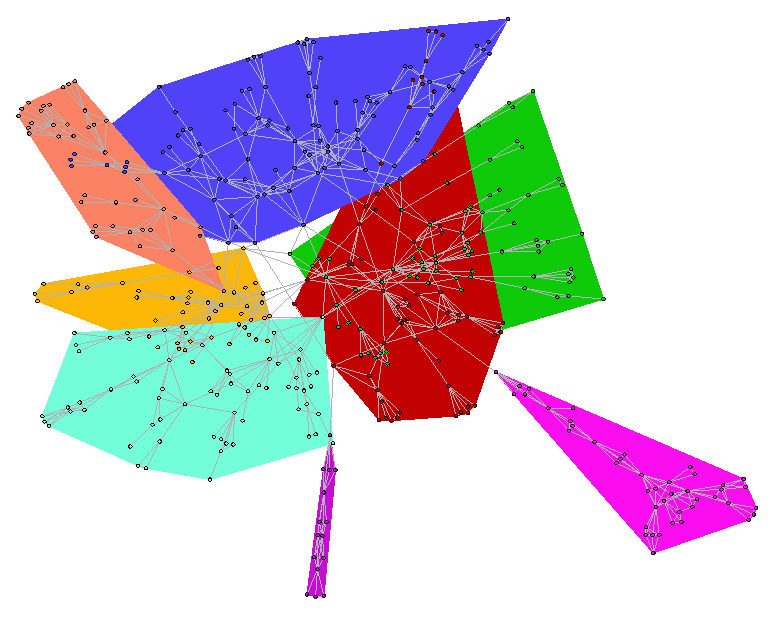
\includegraphics[height=4.00in]{cover/network-um-nsf-9-99-10-09.eps}}

%  cover/network-um-nsf-9-99-10-09.eps cover/network-um-nsf-9-99-10-09-nodes.eps

% \begin{flushright}
% \vspace*{2.0in}
% \begin{spacing}{3}
% {\huge Python for Informatics}\\
% {\Large Exploring Information}\\
% \end{spacing}

% \vspace{0.25in}

% Version \theversion

% \vfill

% \end{flushright}

%--verso------------------------------------------------------

\blankpage
\blankpage
%\clearemptydoublepage
%\pagebreak
%\thispagestyle{empty}
%\vspace*{6in}

%--title page--------------------------------------------------
\pagebreak
\thispagestyle{empty}

\begin{flushright}
\vspace*{2.0in}

\begin{spacing}{3}
{\huge Python for Informatics}\\
{\Large Exploring Information}
\end{spacing}

\vspace{0.25in}

Version \theversion

\vspace{0.5in}


{\Large
Charles Severance\\
}


\vspace{2.25in}

\centerline{
\includegraphics[width=1in]{figs2/by-sa.eps}}
\vfill

\end{flushright}


%--copyright--------------------------------------------------
\pagebreak
\thispagestyle{empty}

{\small
Copyright \copyright ~2009, 2010 Charles Severance.


Printing history:

\begin{description}

\item[December 2009:] Begin to 
produce 
\emph{Python for Informatics: Exploring Information}
by re-mixing
\emph{Think Python: How to Think Like
a Computer Scientist}

\item[June 2008:] Major revision, changed title to
\emph{Think Python: How to Think Like
a Computer Scientist}.

\item[August 2007:] Major revision, changed title to
\emph{How to Think Like a (Python) Programmer}.

\item[April 2002:] First edition of \emph{How to Think Like
a Computer Scientist}.

\end{description}

\vspace{0.2in}

% \begin{flushleft}
% Green Tea Press       \\
% 9 Washburn Ave \\
% Needham MA 02492
% \end{flushleft}

This work is licensed under a 
Creative Commons Attribution-Share Alike 3.0 Unported License.  This license is 
available at
\url{creativecommons.org/licenses/by-sa/3.0/}.

The original form of this book is \LaTeX\ source code.  Compiling this
\LaTeX\ source has the effect of generating a device-independent
representation of a textbook, which can be converted to other formats
and printed.

The \LaTeX\ source for the 
\emph{Think Python: How to Think Like
a Computer Scientist}
version of this book is available from
\url{http://www.thinkpython.com}.

The \LaTeX\ source for the 
\emph{Python for Informatics: Exploring Information}
version of the book is available from 
\url{http://source.sakaiproject.org/contrib/csev/trunk/pyinf/}.

The cover image shows social connectivity of NSF grant investigators 
at the University of Michigan
from September 1999 through October 2010 and was provided
by Eric Hofer and visualized using 
the GUESS software developed by Eytan Adar,
both of the University of Michigan.  The cover design is
by Terri Geitgey of the University of Michigan Library.
\vspace{0.2in}

} % end small

\end{latexonly}


% HTMLONLY

\begin{htmlonly}

% TITLE PAGE FOR HTML VERSION

{\Large \thetitle}

{\large 
Charles Severance}

Version \theversion

\setcounter{chapter}{-1}

\end{htmlonly}

\chapter{Preface}

\section*{Python for Informatics: Remixing an Open Book}

It is quite natural for academics who are continuously told to 
``publish or perish'' to want to always create something from scratch
that is their own fresh creation.   This book is an 
experiment in not starting from scratch, but instead ``re-mixing''
the book titled
\emph{Think Python: How to Think Like
a Computer Scientist}
written by Allen B. Downey, Jeff Elkner and others.

In December of 2009, I was preparing to teach
{\bf SI502 - Networked Programming} at the University of Michigan
for the fifth semester in a row and decided it was time
to write a Python textbook that focused on exploring data
instead of understanding algorithms and abstractions.
My goal in SI502 is to teach people life-long data handling 
skills using Python.  Few of my
students were planning to be be professional 
computer programmers.  Instead, they
planned be librarians, managers, lawyers, biologists, economists, etc. 
who happened to want to skillfully use technology in their chosen field.

I never seemed to find the perfect data-oriented Python
book for my course so I set out 
to write just such a book.  Luckily at a faculty meeting three weeks
before I was about to start my new book from scratch over 
the holiday break, 
Dr. Atul Prakash showed me the \emph{Think Python} book which he had
used to teach his Python course that semester.  
It is a well-written Computer Science text with a focus on 
short, direct explanations and ease of learning.  

The overall book structure
has been changed to get to doing data analysis problems as quickly as
possible and have a series of running examples and exercises 
about data analysis from the very beginning.  

The first 10 chapters are similar to the \emph{Think Python} book
but there have been some changes.  Nearly all number-oriented
exercises have been replaced with data-oriented exerises.
Topics are presented in the order to needed to build increasingly
sophisticated data analysis solutions.  Some topics like {\tt try} and
{\tt except} are pulled forward and presented as part of the chapter
on conditionals while other concepts like functions are left until 
they are needed to handle program complexity rather introduced 
as an early lesson in abstraction.  The word ``recursion'' does not 
appear in the book at all.

In chapters 11-15, nearly all of the material is brand new, focusing
on real-world uses and simple examples of Python for data analysis 
including regular expressons for searching and parsing, 
automating tasks on your computer, retrieving data across 
the network, scraping web pages for data, 
using web services, parsing XML data, and creating 
and using databases using Structured Query Language.

The ultimate goal of all of these changes is a shift from a 
Computer Science to an Informatics
focus is to only include topics into a first technology 
class that can be applied even if one chooses not to 
become a professional programmer.

Students who find this book interesting and want to further explore
should look at Allen B. Downey's \emph{Think Python} book.  Because there
is a lot of overlap between the two books,
students will quickly pick up skills in the additional
areas of computing in general and computational thinking 
that are covered in \emph{Think Python}.
And given that the books have a similar writing style and at times
have identical text and examples, you should be 
able to move quickly through \emph{Think Python} with a minimum of effort.

\index{Creative Commons License}
\index{CC-BY-SA}
\index{BY-SA}
As the copyright holder of \emph{Think Python},
Allen has given me permission to change the book's license 
from the
GNU Free Documentation License 
to the more recent
Creative Commons Attribution --- Share Alike
license.
This follows a general shift in open documentation licenses moving 
from the GFDL to the CC-BY-SA (i.e. Wikipedia).
Using the CC-BY-SA license maintains the book's 
strong copyleft tradition while making it even more straightforward 
for new authors to reuse this material as they see fit.

I feel that this book serves an example of why open 
materials are so important to the future of education,
and want to thank Allen B. Downey and Cambridge University
Press for their forward looking decision to make the book available
under an open Copyright.   I hope they are pleased with the 
results of my efforts and I hope that you the reader are pleased with
\emph{our} collective efforts.

Charles Severance\\
www.dr-chuck.com\\
Ann Arbor, MI, USA\\
July 25, 2010

Charles Severance is a 
Clinical Associate Professor 
at the University of Michigan School of Information.

\section*{Preface for ``Think Python''}

\subsection*{The strange history of ``Think Python''}

(Allen B. Downey)

In January 1999 I was preparing to teach an introductory programming
class in Java.  I had taught it three times and I was getting
frustrated.  The failure rate in the class was too high and, even for
students who succeeded, the overall level of achievement was too low.

One of the problems I saw was the books.  
They were too big, with too much unnecessary detail about Java, and
not enough high-level guidance about how to program.  And they all
suffered from the trap door effect: they would start out easy,
proceed gradually, and then somewhere around Chapter 5 the bottom would
fall out.  The students would get too much new material, too fast,
and I would spend the rest of the semester picking up the pieces.

Two weeks before the first day of classes, I decided to write my
own book.  
My goals were:

\begin{itemize}

\item Keep it short.  It is better for students to read 10 pages
than not read 50 pages.

\item Be careful with vocabulary.  I tried to minimize the jargon
and define each term at first use.

\item Build gradually. To avoid trap doors, I took the most difficult
topics and split them into a series of small steps. 

\item Focus on programming, not the programming language.  I included
the minimum useful subset of Java and left out the rest.

\end{itemize}

I needed a title, so on a whim I chose \emph{How to Think Like
a Computer Scientist}.

My first version was rough, but it worked.  Students did the reading,
and they understood enough that I could spend class time on the hard
topics, the interesting topics and (most important) letting the
students practice.

I released the book under the GNU Free Documentation License,
which allows users to copy, modify, and distribute the book.

\index{GNU Free Documentation License}
\index{Free Documentation License, GNU}

What happened next is the cool part.  Jeff Elkner, a high school
teacher in Virginia, adopted my book and translated it into
Python.  He sent me a copy of his translation, and I had the
unusual experience of learning Python by reading my own book.

Jeff and I revised the book, incorporated a case study by
Chris Meyers, and in 2001 we released \emph{How to Think Like
a Computer Scientist: Learning with Python}, also under
the GNU Free Documentation License.
As Green Tea Press, I published the book and started selling
hard copies through Amazon.com and college book stores.
Other books from Green Tea Press are available at
\url{greenteapress.com}.

In 2003 I started teaching at Olin College and I got to teach
Python for the first time.  The contrast with Java was striking.
Students struggled less, learned more, worked on more interesting
projects, and generally had a lot more fun.

Over the last five years I have continued to develop the book,
correcting errors, improving some of the examples and
adding material, especially exercises.  In 2008 I started work
on a major revision---at the same time, I was
contacted by an editor at Cambridge University Press who
was interested in publishing the next edition.  Good timing!

I hope you enjoy working with this book, and that it helps
you learn to program and think, at least a little bit, like
a computer scientist.

\subsection*{Acknowledgements for ``Think Python''}

(Allen B. Downey)

First and most importantly, I thank Jeff Elkner, who
translated my Java book into Python, which got this project
started and introduced me to what has turned out to be my
favorite language.

I also thank Chris Meyers, who contributed several sections
to \emph{How to Think Like a Computer Scientist}.

And I thank the Free Software Foundation for developing
the GNU Free Documentation License, which helped make
my collaboration with Jeff and Chris possible.

\index{GNU Free Documentation License}
\index{Free Documentation License, GNU}

I also thank the editors at Lulu who worked on
\emph{How to Think Like a Computer Scientist}.

I thank all the students who worked with earlier
versions of this book and all the contributors (listed
in an Appendix) who sent in corrections and suggestions.

And I thank my wife, Lisa, for her work on this book, and Green
Tea Press, and everything else, too.

Allen B. Downey \\
Needham MA\\

Allen Downey is an Associate Professor of Computer Science at 
the Franklin W. Olin College of Engineering.


\clearemptydoublepage

% TABLE OF CONTENTS
\begin{latexonly}

\tableofcontents

\clearemptydoublepage

\end{latexonly}

% START THE BOOK
\mainmatter

\chapter{Why should you learn to write programs?}

Writing programs (or programming) is a very creative 
and rewarding activity.  You can write programs for 
many reasons ranging from making your living to solving
a difficult data analysis problem to having fun to helping
someone else solve a problem.  This book assumes that 
\emph{everyone} needs to know how to program and that once 
you know how to program, you will figure out what you want 
to do with your newfound skills.  

We are surrounded in our daily lives with computers ranging 
from laptops to cell phones.  We can think of these computers
as our ``personal assistants'' who can take care of many things
on our behalf.  The hardware in our current-day computers 
is essentially built to continuously ask us the question, 
``What would you like me to do next?''.

\beforefig
\centerline{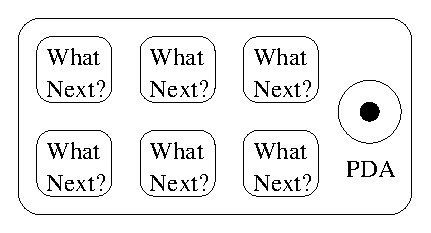
\includegraphics[height=1.00in]{figs2/pda.eps}}
\afterfig

Programmers add an operating system and a set of applications
to the hardware and we end up with a Personal Digital
Assistant that is quite helpful and capable of helping
many different things.

Our computers are fast and have vast amounts of memory and 
could be very helpful to us if we only knew the language to
speak to explain to the computer what we would like it to 
``do next''.  If we knew this language we could tell the 
computer to do tasks on our behalf that were repetitive.  
Interestingly, the kinds of things computers can do best
are often the kinds of things that we humans find boring
and mind-numbing.

For example, look at the first three paragraphs of this
chapter and tell me the most commonly used word and how
many times the word is used.  While you were able to read
and understand the words in a few seconds, counting them
is almost painful because it is not the kind of problem 
that human minds are designed to solve.  For a computer
the opposite is true, reading and understanding text 
from a piece of paper is hard for a computer to do 
but counting the words and telling you how many times
the most used word was used is very easy for the
computer:

\beforeverb
\begin{verbatim}
python words.py
Enter file:words.txt
to 16
\end{verbatim}
\afterverb
%
Our ``personal information analysis assistant'' quickly 
told us that the word ``to'' was used sixteen times in the
first three paragraphs of this chapter.

This very fact that computers are good at things 
that humans are not is why you need to become
skilled at talking ``computer language''.  Once you learn
this new language, you can delegate mundane tasks
to your partner (the computer), leaving more time 
for you to do the 
things that you are uniquely suited for.  You bring 
creativity, intuition, and inventiveness to this
partnership.  

\section{Creativity and motivation}

While this book is not intended for professional programmers, professional
programming can be a very rewarding job both financially and personally.
Building useful, elegant, and clever programs for others to use is a very
creative activity.  Your computer or Personal Digital Assistant (PDA) 
usually contains many different programs from many different groups of 
programmers, each competing for your attention and interest.  They try 
their best to meet your needs and give you a great user experience in the
process.   In some situations, when you choose a piece of software, the 
programmers are directly compensated because of your choice.

If we think of programs as the creative output of groups of programmers,
perhaps the following figure is a more sensible version of our PDA:

\beforefig
\centerline{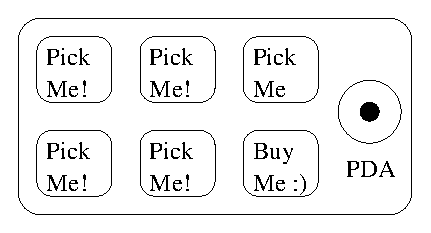
\includegraphics[height=1.00in]{figs2/pda2.eps}}
\afterfig

For now, our primary motivation is not to make money or please end-users, but
instead for us to be more productive in handling the data and 
information that we will encounter in our lives.
When you first start, you will be both the programmer and end-user of
your programs.  As you gain skill as a programmer and
programming feels more creative to you, your thoughts may turn
toward developing programs for others.

\section{Computer hardware architecture}
\index{hardware}
\index{hardware!architecture}

Before we start learning the language we 
speak to give instructions to computers to 
develop software, we need to learn a small amount about 
how computers are built.  If you were to take
apart your computer or cell phone and look deep
inside, you would find the following parts:

\beforefig
\centerline{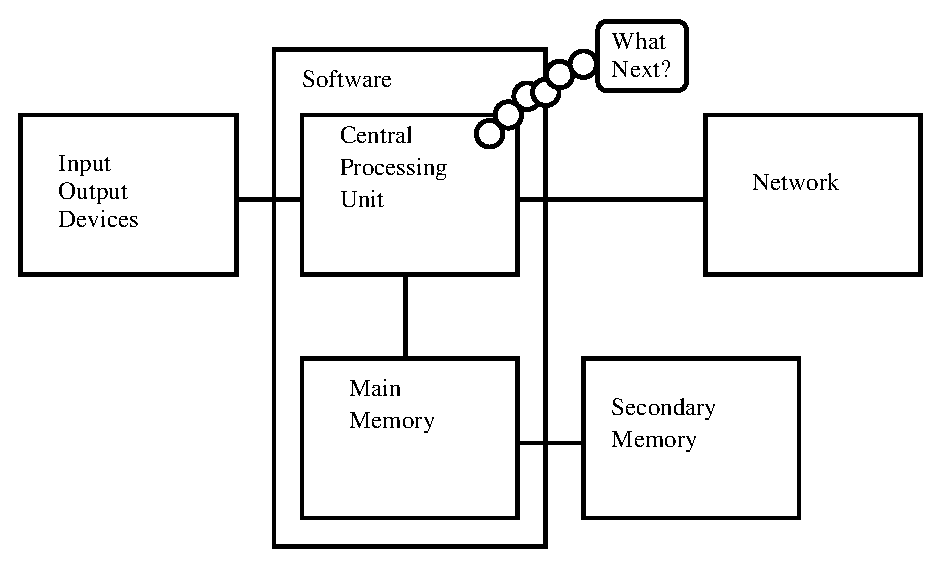
\includegraphics[height=2.50in]{figs2/arch.eps}}
\afterfig

The high-level definitions of these parts are as follows:

\begin{itemize}

\item The {\bf Central Processing Unit} (or CPU) is 
that part of the computer that is built to be obsessed 
with ``what is next?''.  If your computer is rated
at 3.0 Gigahertz, it means that the CPU will ask ``What next?''
three billion times per second.  You are going to have to 
learn how to talk fast to keep up with the CPU.

\item The {\bf Main Memory} is used to store information
that the CPU needs in a hurry.  The main memory is nearly as 
fast as the CPU.  But the information stored in the main
memory vanishes when the computer is turned off.

\item The {\bf Secondary Memory} is also used to store
information, but it is much slower than the main memory.
The advantage of the secondary memory is that it can
store information even when there is no power to the
computer.  Examples of secondary memory are disk drives
or flash memory (typically found in USB sticks and portable
music players).

\item The {\bf Input and Output Devices} are simply our
screen, keyboard, mouse, microphone, speaker, touchpad, etc.  
They are all of the ways we interact with the computer.

\item These days, most computers also have a
{\bf Network Connection} to retrieve information over a network.
We can think of the network as a very slow place to store and
retrieve data that might not always be ``up''.  So in a sense,
the network is a slower and at times unreliable form of
{\bf Secondary Memory}

\end{itemize}

While most of the detail of how these components work is best left 
to computer builders, it helps to have some terminology
so we can talk about these different parts as we write our programs.

As a programmer, your job is to use and orchestrate 
each of these resources to solve the problem that you need solving
and analyze the data you need.  As a programmer you will 
mostly be ``talking'' to the CPU and telling it what to 
do next.  Sometimes you will tell the CPU to use the main memory,
secondary memory, network, or the input/output devices.

\beforefig
\centerline{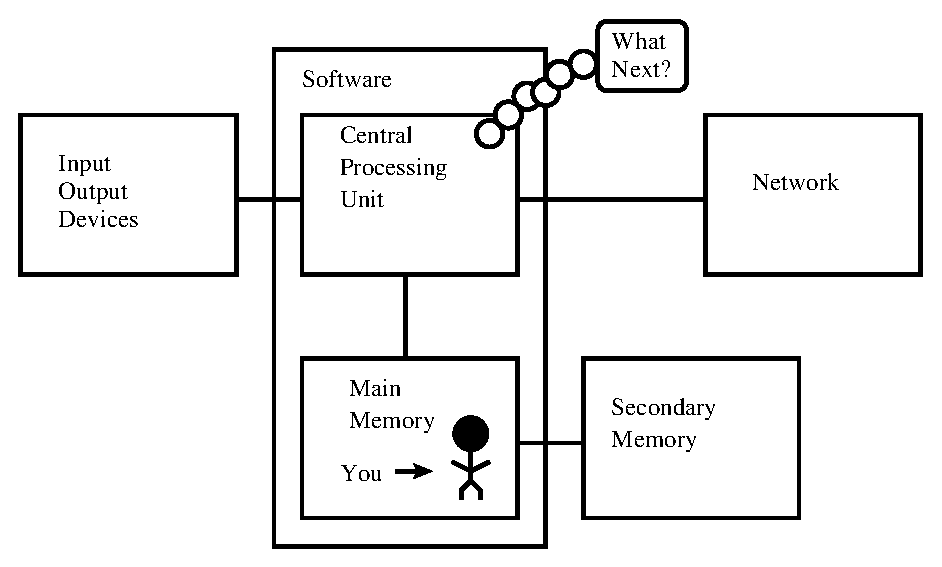
\includegraphics[height=2.50in]{figs2/arch2.eps}}
\afterfig

You need to be the person who answers the CPU's ``What next?'' 
question.  But it would be very uncomfortable to shrink you 
down to 5mm tall and insert you into the computer just so you 
could issue a command three billion times per second.  So instead,
you must write down your instructions in advance.
We call these stored instructions a {\bf program} and the act 
of writing these instructions down and getting the instructions to 
be correct {\bf programming}.

\section{Understanding programming}

In the rest of this book, we will try to turn you into a person
who is skilled in the art of programming.  In the end you will be a 
{\bf programmer} --- perhaps not a professional programmer but 
at least you will have the skills to look at a data/information
analysis problem and develop a program to solve the problem.

\index{problem solving}

In a sense, you need two skills to be a programmer:

\begin{itemize}

\item First you need to know the programming language (Python) -
you need to know the vocabulary and the grammar.  You need to be able 
spell the words in this new language properly and how to construct 
well-formed ``sentences'' in this new languages.

\item Second you need to ``tell a story''.  In writing a story,
you combine words and sentences to convey an idea to the reader. 
There is a skill and art in constructing the story and skill in
story writing is improved by doing some writing and getting some
feedback.  In programming, our program is the ``story'' and the 
problem you are trying to solve is the ``idea''.

\end{itemize}

Once you learn one programming language such as Python, you will 
find it much easier to learn a second programming language such
as JavaScript or C++.  The new programming language has very different 
vocabulary and grammar but once you learn problem solving skills, 
they will be the same across all programming languages.

You will learn the ``vocabulary'' and ``sentences'' of Python pretty quickly.
It will take longer for you to be able to write a coherent program
to solve a brand new problem.  We teach programming much like we teach
writing.  We start reading and explaining programs and then we write 
simple programs and then write increasingly complex programs over time.
At some point you ``get your muse'' and see the patterns on your own
and can see more naturally how to take a problem and 
write a program that solves that problem.  And once you get 
to that point, programming becomes a very pleasant and creative process.  

We start with the vocabulary and structure of Python programs.  Be patient
as the simple examples remind you of when you started reading for the first
time. 

\section{The Python programming language}
\index{programming language}
\index{language!programming}

The programming language you will learn is Python. Python is
an example of a {\bf high-level language}; some other high-level languages
you might have heard of are C, C++, Perl, Java, Ruby, and JavaScript. 

There are
also {\bf low-level languages}, sometimes referred to as ``machine
languages'' or ``assembly languages.''  Loosely speaking, computers
can only execute programs written in low-level languages.  So
programs written in a high-level language have to be processed before
they can run.  This extra processing takes some time, which is a small
disadvantage of high-level languages.

\index{portability}
\index{high-level language}
\index{low-level language}
\index{language!high-level}
\index{language!low-level}

However, the advantages are enormous.  First, it is much easier to program
in a high-level language.  Programs written in a high-level language
take less time to write, they are shorter and easier to read, and they
are more likely to be correct.  Second, high-level languages are {\bf
portable}, meaning that they can run on different kinds of computers
with few or no modifications.  Low-level programs can run on only one
kind of computer and have to be rewritten to run on another.

Due to these advantages, almost all programs are written in high-level
languages.  Low-level languages are used only for a few specialized
applications.

\index{compile}
\index{interpret}

Two kinds of programs process high-level languages
into low-level languages: {\bf interpreters} and {\bf compilers}.
An interpreter reads a high-level program and executes it, meaning that it
does what the program says.  It processes the program a little at a time,
alternately reading lines and performing computations.

\beforefig
\centerline{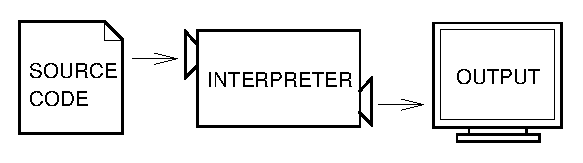
\includegraphics[height=0.77in]{figs/interpret.eps}}
\afterfig

\index{source code}
\index{object code}
\index{executable}

A compiler reads the program and translates it completely before the
program starts running.  In this context, the high-level program is
called the {\bf source code}, and the translated program is called the
{\bf object code}, {\bf machine code} or the {\bf executable}.  
Once a program is compiled, you can execute it 
repeatedly without further translation.

\beforefig
\centerline{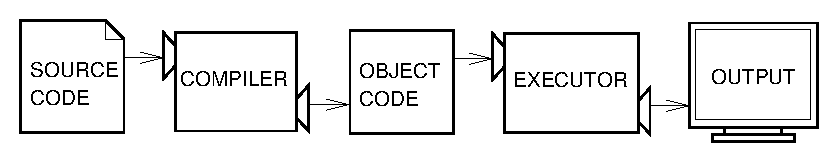
\includegraphics[height=0.77in]{figs/compile.eps}}
\afterfig

Python is considered an interpreted language because Python programs
are executed by an interpreter.  There are two ways to use the
interpreter: {\bf interactive mode} and {\bf script mode}. 

To start interactive mode, you have to run the Python interpreter
program.
In a UNIX or Windows command window, you would type {\tt python}
to run the Python interpreter.

In interactive mode, you type Python programs and the interpreter prints
the result:

\index{interactive mode}
\index{script mode}

\beforeverb
\begin{verbatim}
>>> 1 + 1
2
>>>
\end{verbatim}
\afterverb
%
The chevron, {\tt >>>}, is the
{\bf prompt} the interpreter uses to indicate that it is ready.  If
you type {\tt 1 + 1}, the interpreter replies {\tt 2}.
The chevron is the Python interpreter's way of asking you, ``What
do you want me to do next?''.  You will notice that as soon as 
Python finishes one statement it immediately is ready for you to type 
another statement.

\index{prompt}

Typing commands into the Python interpreter is a great way to experiment
with Python's features, but it is a bad way to type in many commands 
to solve a more complex problem.  When we want to write a program, 
we use a text editor to write the Python instructions into a file,
which is called a {\bf script}.  By
convention, Python scripts have names that end with {\tt .py}.

\index{script}

To execute the script, you have to tell the interpreter the name of
the file.  In a UNIX or Windows command window, you would type {\tt python
dinsdale.py}.  In other development environments, the details of
executing scripts are different.  You can find instructions for
your environment at the Python Website \url{python.org}.

\index{testing!interactive mode}

Working in interactive mode is convenient for testing small pieces of
code because you can type and execute them immediately.  But for
anything more than a few lines, you should save your code
as a script so you can modify and execute it in the future.


\section{What is a program?}

A {\bf program} is a sequence of instructions that specifies how to
perform a computation.  The computation might be something
mathematical, such as solving a system of equations or finding the
roots of a polynomial, but it can also be a symbolic computation, such
as searching and replacing text in a document or (strangely enough)
compiling a program.

\index{program}

The details look different in different languages, but a few basic
instructions appear in just about every language:

\begin{description}

\item[input:] Get data from the keyboard, a file, or some
other device, pausing if necessary.

\item[output:] Display data on the screen or send data to a
file or other device.

\item[sequential execution:] Perform statements one after
another in the order they are encountered in the script.

\item[conditional execution:] Check for certain conditions and
execute or skip a sequence of statements.

\item[repeated execution:] Perform some set of statements 
repeatedly, usually with
some variation.

\item[reuse:] Write a set of instructions once and give them a name
and then reuse those instructions as needed throughout your program.

\end{description}

Believe it or not, that's pretty much all there is to it.  Every
program you've ever used, no matter how complicated, is made up of
instructions that look pretty much like these.  So you can think of
programming as the process of breaking a large, complex task
into smaller and smaller subtasks until the subtasks are
simple enough to be performed with one of these basic instructions.

\section{What is debugging?}
\index{debugging}
\index{bug}

Programming is error-prone.  For whimsical reasons, programming errors
are called {\bf bugs} and the process of tracking them down is called
{\bf debugging}.

\index{debugging}
\index{bug}

Three kinds of errors can occur in a program: syntax errors, runtime 
errors, and semantic errors. It is useful
to distinguish between them in order to track them down more quickly.

\subsection{Syntax errors}
\index{syntax error}
\index{error!syntax}
\index{error message}

Python can only execute a program if the syntax is
correct; otherwise, the interpreter displays an error message.
{\bf Syntax} refers to the structure of a program and the rules about
that structure. \index{syntax} 
For example, parentheses have to come in matching pairs, so
{\tt (1 + 2)} is legal, but {\tt 8)} is a {\bf syntax error}.

\index{parentheses!matching}
\index{syntax}

In English readers can tolerate most syntax errors, which is why we
can read certain abstract poetry.
Python is not so forgiving.  If there is a single syntax error
anywhere in your program, Python will display an error message and quit,
and you will not be able to run your program. During the first few
weeks of your programming career, you will probably spend a lot of
time tracking down syntax errors.  As you gain experience, you will
make fewer errors and find them faster.

\subsection{Runtime errors}
\label{runtime}
\index{runtime error}
\index{error!runtime}
\index{exception}
\index{safe language}
\index{language!safe}

The second type of error is a runtime error, so called because the
error does not appear until after the program has started running.
These errors are also called {\bf exceptions} because they usually
indicate that something exceptional (and bad) has happened.

Runtime errors are rare in the simple programs you will see in the
first few chapters, so it might be a while before you encounter one.


\subsection{Semantic errors}
\index{semantics}
\index{semantic error}
\index{error!semantic}
\index{error message}

The third type of error is the {\bf semantic error}.  If there is a
semantic error in your program, it will run successfully in the sense
that the computer will not generate any error messages, but it will
not do the right thing.  It will do something else.  Specifically, it
will do what you told it to do but not what you meant for it to do.

The problem is that the program you wrote is not the program you
wanted to write.  The meaning of the program (its semantics) is wrong.
Identifying semantic errors can be tricky because it requires you to work
backward by looking at the output of the program and trying to figure
out what it is doing.

\subsection{Experimental debugging}

One of the most important skills you will acquire is debugging.
Although it can be frustrating, debugging is one of the most
intellectually rich, challenging, and interesting parts of
programming.

\index{experimental debugging}
\index{debugging!experimental}

In some ways, debugging is like detective work.  You are confronted
with clues, and you have to infer the processes and events that led
to the results you see.

Debugging is also like an experimental science.  Once you have an idea
about what is going wrong, you modify your program and try again.  If
your hypothesis was correct, then you can predict the result of the
modification, and you take a step closer to a working program.  If
your hypothesis was wrong, you have to come up with a new one.  As
Sherlock Holmes pointed out, ``When you have eliminated the
impossible, whatever remains, however improbable, must be the truth.''
(A. Conan Doyle, \emph{The Sign of Four})

\index{Holmes, Sherlock}
\index{Doyle, Arthur Conan}

For some people, programming and debugging are the same thing.  That
is, programming is the process of gradually debugging a program until
it does what you want.  The idea is that you should start with a
program that does \emph{something} and make small modifications,
debugging them as you go, so that you always have a working program.

For example, Linux is an operating system that contains thousands of
lines of code, but it started out as a simple program Linus Torvalds
used to explore the Intel 80386 chip.  According to Larry Greenfield,
``One of Linus's earlier projects was a program that would switch
between printing AAAA and BBBB.  This later evolved to Linux.''
(\emph{The Linux Users' Guide} Beta Version 1).

\index{Linux}

Later chapters will make more suggestions about debugging and other
programming practices.

\section{Building ``sentences'' in Python}
\index{formal language}
\index{natural language}
\index{language!formal}
\index{language!natural}

The rules (or grammar) of Python are simpler and more precise than 
the rules of a natural language that we use to speak and write.

{\bf Natural languages} are the languages people speak,
such as English, Spanish, and French.  They were not designed
by people (although people try to impose some order on them);
they evolved naturally.

{\bf Formal languages} are languages that are designed by people for
specific applications.  For example, the notation that mathematicians
use is a formal language that is particularly good at denoting
relationships among numbers and symbols.  Chemists use a formal
language to represent the chemical structure of molecules.  And
most importantly:

\begin{quote}
{\bf Programming languages are formal languages that have been
designed to express computations.}
\end{quote}

Formal languages tend to have strict rules about syntax.  For example,
$3 + 3 = 6$ is a syntactically correct mathematical statement, but 
$3 + + 3 @ 6$ is not.  $H_2O$ is a syntactically correct
chemical formula, but $_2Zz$ is not.

Syntax rules come in two flavors, pertaining to {\bf tokens} and
structure.  Tokens are the basic elements of the language, such as
words, numbers, and chemical elements.  One of the problems with $3 +
+ 3 @ 6$ is that @ is not a legal token in mathematics
(at least as far as I know).  Similarly, $_2Zz$ is not legal because
there is no element with the abbreviation $Zz$.

\index{token}
\index{structure}

The second type of syntax error pertains to the structure of a
statement; that is, the way the tokens are arranged.  The statement $3
+ + 3 @ 6$ is illegal because even though $+$ is a legal token and 
you can have more than one plus in an exression, you cannot have one
right after another. 
Similarly,
in a chemical formula the subscript comes after the element name, not
before.

\begin{ex}
Write a well-structured English
sentence with invalid tokens in it.  Then write another sentence
with all valid tokens but with invalid structure.
\end{ex}

When you read a sentence in English or a statement in a formal
language, you have to figure out what the structure of the sentence is
(although in a natural language you do this subconsciously).  This
process is called {\bf parsing}.

\index{parse}

For example, when you hear the sentence, ``The penny dropped,'' you
understand that ``the penny'' is the subject and ``dropped'' is the
predicate.  Once you have parsed a sentence, you can figure out what it
means, or the semantics of the sentence.  Assuming that you know
what a penny is and what it means to drop, you will understand the
general implication of this sentence.

Although formal and natural languages have many features in
common---tokens, structure, syntax, and semantics---there are some
differences:

\index{ambiguity}
\index{redundancy}
\index{literalness}

\begin{description}

\item[ambiguity:] Natural languages are full of ambiguity, which
people deal with by using contextual clues and other information.
Formal languages are designed to be nearly or completely unambiguous,
which means that any statement has exactly one meaning,
regardless of context.

\item[redundancy:] In order to make up for ambiguity and reduce
misunderstandings, natural languages employ lots of
redundancy.  As a result, they are often verbose.  Formal languages
are less redundant and more concise.

\item[literalness:] Natural languages are full of idiom and metaphor.
If I say, ``The penny dropped,'' there is probably no penny and
nothing dropping\footnote{This idiom means that someone realized something
after a period of confusion.}.  Formal languages
mean exactly what they say.

\end{description}

People who grow up speaking a natural language---everyone---often have a
hard time adjusting to formal languages.  In some ways, the difference
between formal and natural language is like the difference between
poetry and prose, but more so:

\index{poetry}
\index{prose}

\begin{description}

\item[Poetry:] Words are used for their sounds as well as for
their meaning, and the whole poem together creates an effect or
emotional response.  Ambiguity is not only common but often
deliberate.

\item[Prose:] The literal meaning of words is more important,
and the structure contributes more meaning.  Prose is more amenable to
analysis than poetry but still often ambiguous.

\item[Programs:] The meaning of a computer program is unambiguous
and literal, and can be understood entirely by analysis of the
tokens and structure.

\end{description}

Here are some suggestions for reading programs (and other formal
languages).  First, remember that formal languages are much more dense
than natural languages, so it takes longer to read them.  Also, the
structure is very important, so it is usually not a good idea to read
from top to bottom, left to right.  Instead, learn to parse the
program in your head, identifying the tokens and interpreting the
structure.  Finally, the details matter.  Small errors in
spelling and punctuation, which you can get away
with in natural languages, can make a big difference in a formal
language.

\section{The first program}
\label{hello}

\index{Hello, World}

Traditionally, the first program you write in a new language
is called ``Hello, World!'' because all it does is display the
words, ``Hello, World!''  In Python, it looks like this:

\beforeverb
\begin{verbatim}
print 'Hello, World!'
\end{verbatim}
\afterverb
%
This is an example of a {\bf print statement}\footnote{In Python 3.0,
  {\tt print} is a function, not a statement, so the syntax is {\tt
    print('Hello, World!')}.  We will get to functions soon!}, which
doesn't actually print anything on paper.  It displays a value on the
screen.  In this case, the result is the words

\index{Python 3.0}

\beforeverb
\begin{verbatim}
Hello, World!
\end{verbatim}
\afterverb
%
The quotation marks in the program mark the beginning and end
of the text to be displayed; they don't appear in the result.

\index{quotation mark}
\index{print statement}
\index{statement!print}

Some people judge the quality of a programming language by the
simplicity of the ``Hello, World!'' program.  By this standard, Python
does about as well as possible.


\section{Debugging}
\index{debugging}

It is a good idea to read this book in front of a computer so you can
try out the examples as you go.  You can run most of the examples in
interactive mode, but if you put the code into a script, it is easier
to try out variations.

Whenever you are experimenting with a new feature, you should try
to make mistakes.  For example, in the ``Hello, world!'' program,
what happens if you leave out one of the quotation marks?  What
if you leave out both?  What if you spell {\tt print} wrong?

\index{error message}

This kind of experiment helps you remember what you read; it also helps
with debugging, because you get to know what the error messages mean.
It is better to make mistakes now and on purpose than later
and accidentally.

Programming, and especially debugging, sometimes brings out strong
emotions.  If you are struggling with a difficult bug, you might 
feel angry, despondent or embarrassed.

There is evidence that people naturally respond to computers as if
they were people\footnote{See Reeves and Nass, {\it The Media
    Equation: How People Treat Computers, Television, and New Media
    Like Real People and Places}.}.  When they work well, we think
of them as teammates, and when they are obstinate or rude, we
respond to them the same way we respond to rude,
obstinate people.

\index{debugging!emotional response}
\index{emotional debugging}

Preparing for these reactions might help you deal with them.
One approach is to think of the computer as an employee with
certain strengths, like speed and precision, and
particular weaknesses, like lack of empathy and inability
to grasp the big picture.

Your job is to be a good manager: find ways to take advantage
of the strengths and mitigate the weaknesses.  And find ways
to use your emotions to engage with the problem,
without letting your reactions interfere with your ability
to work effectively.

Learning to debug can be frustrating, but it is a valuable skill
that is useful for many activities beyond programming.  At the
end of each chapter there is a debugging section, like this one,
with my thoughts about debugging.  I hope they help!


\section{Glossary}

\begin{description}

\item[bug:]  An error in a program.
\index{bug}

\item[central processing unit:] The heart of any computer.  It is what
runs the software that we write; also called ``CPU'' or ``the processor''.
\index{central processing unit}
\index{CPU}

\item[compile:]  To translate a program written in a high-level language
into a low-level language all at once, in preparation for later
execution.
\index{compile}

\item[debugging:]  The process of finding and removing any of the
three kinds of programming errors.
\index{debugging}

\item[exception:]  An error that is detected while the program is running.
\index{exception}

\item[executable:]  Another name for object code that is ready
to be executed.
\index{executable}

\item[formal language:]  Any one of the languages that people have designed
for specific purposes, such as representing mathematical ideas or
computer programs; all programming languages are formal languages.
\index{formal language}

\item[high-level language:]  A programming language like Python that
is designed to be easy for humans to read and write.
\index{high-level language}

\item[interactive mode:] A way of using the Python interpreter by
typing commands and expressions at the prompt.
\index{interactive mode}

\item[interpret:]  To execute a program in a high-level language
by translating it one line at a time.
\index{interpret}

\item[low-level language:]  A programming language that is designed
to be easy for a computer to execute; also called ``machine code'' or
``assembly language.''
\index{low-level language}

\item[machine code:]  The lowest level language for software which 
is the language that is directly executed by the central processing unit 
(CPU).
\index{machine code}

\item[main memory:] Stores programs and data.  Main memory loses 
its information when the power is turned off.
\index{main memory}

\item[natural language:]  Any one of the languages that people speak that
evolved naturally.
\index{natural language}

\item[object code:]  The output of the compiler after it translates
the program.
\index{object code}

\item[parse:]  To examine a program and analyze the syntactic structure.
\index{parse}

\item[portability:]  A property of a program that can run on more
than one kind of computer.
\index{portability}

\item[print statement:]  An instruction that causes the Python
interpreter to display a value on the screen.
\index{print statement}
\index{statement!print}

\item[problem solving:]  The process of formulating a problem, finding
a solution, and expressing the solution.
\index{problem solving}

\item[program:] A set of instructions that specifies a computation.
\index{program}

\item[prompt:] Characters displayed by the interpreter to indicate
that it is ready to take input from the user.
\index{prompt}

\item[secondary memory:] Stores programs and data and retains its 
information even when the power is turned off.  Generally slower 
than main memory.  Examples of secondary memory include disk 
drives and flash member in USB sticks.
\index{secondary memory}

\item[script:] A program stored in a file (usually one that will be
interpreted).
\index{script}

\item[script mode:] A way of using the Python interpreter to read
and execute statements in a script.
\index{script mode}

\item[semantics:]  The meaning of a program.
\index{semantics}

\item[semantic error:]   An error in a program that makes it do something
other than what the programmer intended.
\index{semantic error}

\item[source code:]  A program in a high-level language before
being compiled.
\index{source code}

\item[syntax:]  The structure of a program.
\index{syntax}

\item[syntax error:]  An error in a program that makes it impossible
to parse (and therefore impossible to interpret).
\index{syntax error}

\item[token:]  One of the basic elements of the syntactic structure of
a program, analogous to a word in a natural language.
\index{token}



\end{description}


\section{Exercises}

\begin{ex}
Use a web browser to go to the Python Website \url{python.org}.
This page contains information about Python and links
to Python-related pages, and it gives you the ability to search
the Python documentation.

For example, if you enter {\tt print} in the search window, the
first link that appears is the documentation of the {\tt print}
statement.  At this point, not all of it will make sense to you,
but it is good to know where it is.

\index{documentation}
\index{python.org}
\end{ex}

\begin{ex}
Start the Python interpreter and type {\tt help()} to start the online
help utility.  Or you can type \verb"help('print')" to get information
about the {\tt print} statement.

If this example doesn't work, you
may need to install additional Python documentation or set an
environment variable; the details depend on your operating system and
version of Python.

\index{help utility}
\end{ex}

\begin{ex}
Start the Python interpreter and use it as a calculator.
Python's syntax for math operations is almost the same as
standard mathematical notation.  For example, the symbols
{\tt +}, {\tt -} and {\tt /} denote addition, subtraction
and division, as you would expect.  The symbol for
multiplication is {\tt *}.

If you run a 10 kilometer race in 43 minutes 30 seconds, what is your
average time per mile?  What is your average speed in miles per hour?
(Hint: there are 1.61 kilometers in a mile).

\index{calculator}
\index{running pace}

\end{ex}

\chapter{Variables, expressions and statements}

\section{Values and types}
\index{value}
\index{type}
\index{string}

A {\bf value} is one of the basic things a program works with,
like a letter or a
number.  The values we have seen so far
are {\tt 1}, {\tt 2}, and
\verb"'Hello, World!'".

These values belong to different {\bf types}:
{\tt 2} is an integer, and \verb"'Hello, World!'" is a {\bf string},
so-called because it contains a ``string'' of letters.
You (and the interpreter) can identify
strings because they are enclosed in quotation marks.

\index{quotation mark}

The {\tt print} statement also works for integers.  We use the 
{\tt python} command to start the interpreter.

\beforeverb
\begin{verbatim}
python
>>> print 4
4
\end{verbatim}
\afterverb
%
If you are not sure what type a value has, the interpreter can tell you.

\beforeverb
\begin{verbatim}
>>> type('Hello, World!')
<type 'str'>
>>> type(17)
<type 'int'>
\end{verbatim}
\afterverb
%
Not surprisingly, strings belong to the type {\tt str} and
integers belong to the type {\tt int}.  Less obviously, numbers
with a decimal point belong to a type called {\tt float},
because these numbers are represented in a
format called {\bf floating-point}.

\index{type}
\index{string type}
\index{type!str}
\index{int type}
\index{type!int}
\index{float type}
\index{type!float}

\beforeverb
\begin{verbatim}
>>> type(3.2)
<type 'float'>
\end{verbatim}
\afterverb
%
What about values like \verb"'17'" and \verb"'3.2'"?
They look like numbers, but they are in quotation marks like
strings.

\index{quotation mark}

\beforeverb
\begin{verbatim}
>>> type('17')
<type 'str'>
>>> type('3.2')
<type 'str'>
\end{verbatim}
\afterverb
%
They're strings.

When you type a large integer, you might be tempted to use commas
between groups of three digits, as in {\tt 1,000,000}.  This is not a
legal integer in Python, but it is legal:

\beforeverb
\begin{verbatim}
>>> print 1,000,000
1 0 0
\end{verbatim}
\afterverb
%
Well, that's not what we expected at all!  Python interprets {\tt
  1,000,000} as a comma-separated sequence of integers, which it
prints with spaces between.

\index{semantic error}
\index{error!semantic}
\index{error message}

This is the first example we have seen of a semantic error: the code
runs without producing an error message, but it doesn't do the
``right'' thing.


\section{Variables}
\index{variable}
\index{assignment statement}
\index{statement!assignment}

One of the most powerful features of a programming language is the
ability to manipulate {\bf variables}.  A variable is a name that
refers to a value.

An {\bf assignment statement} creates new variables and gives
them values:

\beforeverb
\begin{verbatim}
>>> message = 'And now for something completely different'
>>> n = 17
>>> pi = 3.1415926535897931
\end{verbatim}
\afterverb
%
This example makes three assignments.  The first assigns a string
to a new variable named {\tt message};
the second assigns the integer {\tt 17} to {\tt n}; the third
assigns the (approximate) value of $\pi$ to {\tt pi}.

\index{state diagram}
\index{diagram!state}

A common way to represent variables on paper is to write the name with
an arrow pointing to the variable's value.  This kind of figure is
called a {\bf state diagram} because it shows what state each of the
variables is in (think of it as the variable's state of mind).
This diagram shows the result of the previous example:

\beforefig
\centerline{
\includegraphics{figs/state2.eps}}
\afterfig

To display the value of a variable, you can use a print statement:

\beforeverb
\begin{verbatim}
>>> print n
17
>>> print pi
3.14159265359
\end{verbatim}
\afterverb
%
The type of a variable is the type of the value it refers to.

\beforeverb
\begin{verbatim}
>>> type(message)
<type 'str'>
>>> type(n)
<type 'int'>
>>> type(pi)
<type 'float'>
\end{verbatim}
\afterverb
%

\section{Variable names and keywords}
\index{keyword}

Programmers generally choose names for their variables that
are meaningful---they document what the variable is used for.

Variable names can be arbitrarily long.  They can contain
both letters and numbers, but they have to begin with a letter.
It is legal to use uppercase letters, but it is a good idea
to begin variable names with a lowercase letter (you'll
see why later).

The underscore character (\verb"_") can appear in a name.
It is often used in names with multiple words, such as
\verb"my_name" or \verb"airspeed_of_unladen_swallow".

\index{underscore character}

If you give a variable an illegal name, you get a syntax error:

\beforeverb
\begin{verbatim}
>>> 76trombones = 'big parade'
SyntaxError: invalid syntax
>>> more@ = 1000000
SyntaxError: invalid syntax
>>> class = 'Advanced Theoretical Zymurgy'
SyntaxError: invalid syntax
\end{verbatim}
\afterverb
%
{\tt 76trombones} is illegal because it does not begin with a letter.
{\tt more@} is illegal because it contains an illegal character, {\tt
@}.  But what's wrong with {\tt class}?

It turns out that {\tt class} is one of Python's {\bf keywords}.  The
interpreter uses keywords to recognize the structure of the program,
and they cannot be used as variable names.

\index{keyword}

Python reserves 31 keywords\footnote{In Python 3.0, {\tt exec} is no
longer a keyword, but {\tt nonlocal} is.} for its use:

\beforeverb
\begin{verbatim}
and       del       from      not       while    
as        elif      global    or        with     
assert    else      if        pass      yield    
break     except    import    print              
class     exec      in        raise              
continue  finally   is        return             
def       for       lambda    try
\end{verbatim}
\afterverb
%
You might want to keep this list handy.  If the interpreter complains
about one of your variable names and you don't know why, see if it
is on this list.

\section{Statements}

A {\bf statement} is a unit of code that the Python interpreter can
execute.  We have seen two kinds of statements: print
and assignment.

\index{statement}
\index{interactive mode}
\index{script mode}

When you type a statement in interactive mode, the interpreter
executes it and displays the result, if there is one.

A script usually contains a sequence of statements.  If there
is more than one statement, the results appear one at a time
as the statements execute.

For example, the script

\beforeverb
\begin{verbatim}
print 1
x = 2
print x
\end{verbatim}
\afterverb
%
produces the output

\beforeverb
\begin{verbatim}
1
2
\end{verbatim}
\afterverb
%
The assignment statement produces no output.


\section{Operators and operands}
\index{operator, arithmetic}
\index{arithmetic operator}
\index{operand}
\index{expression}

{\bf Operators} are special symbols that represent computations like
addition and multiplication.  The values the operator is applied to
are called {\bf operands}.

The operators {\tt +}, {\tt -}, {\tt *}, {\tt /} and {\tt **}
perform addition, subtraction, multiplication, division and
exponentiation, as in the following examples:

\beforeverb
\begin{verbatim}
20+32   hour-1   hour*60+minute   minute/60   5**2   (5+9)*(15-7)
\end{verbatim}
\afterverb
%
The division operator might not do what you expect:

\beforeverb
\begin{verbatim}
>>> minute = 59
>>> minute/60
0
\end{verbatim}
\afterverb
%
The value of {\tt minute} is 59, and in conventional arithmetic 59
divided by 60 is 0.98333, not 0.  The reason for the discrepancy is
that Python is performing {\bf floor division}\footnote{In Python 3.0,
the result of this division is a {\tt float}.  
In Python 3.0, the new operator
{\tt //} performs integer division.}.

\index{Python 3.0}
\index{floor division}
\index{floating-point division}
\index{division!floor}
\index{division!floating-point}

When both of the operands are integers, the result is also an
integer; floor division chops off the fraction
part, so in this example it rounds down to zero.

If either of the operands is a floating-point number, Python performs
floating-point division, and the result is a {\tt float}:

\beforeverb
\begin{verbatim}
>>> minute/60.0
0.98333333333333328
\end{verbatim}
\afterverb


\section{Expressions}

An {\bf expression} is a combination of values, variables, and operators.
A value all by itself is considered an expression, and so is
a variable, so the following are all legal expressions
(assuming that the variable {\tt x} has been assigned a value):

\index{expression}
\index{evaluate}

\beforeverb
\begin{verbatim}
17
x
x + 17
\end{verbatim}
\afterverb
%
If you type an expression in interactive mode, the interpreter
{\bf evaluates} it and displays the result:

\beforeverb
\begin{verbatim}
>>> 1 + 1
2
\end{verbatim}
\afterverb
%
But in a script, an expression all by itself doesn't
do anything!  This is a common
source of confusion for beginners.

\begin{ex}
Type the following statements in the Python interpreter to see
what they do:

\beforeverb
\begin{verbatim}
5
x = 5
x + 1
\end{verbatim}
\afterverb
%
\end{ex}


\section{Order of operations}
\index{order of operations}
\index{rules of precedence}
\index{PEMDAS}

When more than one operator appears in an expression, the order of
evaluation depends on the {\bf rules of precedence}.  For
mathematical operators, Python follows mathematical convention.
The acronym {\bf PEMDAS} is a useful way to
remember the rules:

\index{parentheses!overriding precedence}

\begin{itemize}

\item {\bf P}arentheses have the highest precedence and can be used 
to force an expression to evaluate in the order you want. Since
expressions in parentheses are evaluated first, {\tt 2 * (3-1)} is 4,
and {\tt (1+1)**(5-2)} is 8. You can also use parentheses to make an
expression easier to read, as in {\tt (minute * 100) / 60}, even
if it doesn't change the result.

\item {\bf E}xponentiation has the next highest precedence, so
{\tt 2**1+1} is 3, not 4, and {\tt 3*1**3} is 3, not 27.

\item {\bf M}ultiplication and {\bf D}ivision have the same precedence,
which is higher than {\bf A}ddition and {\bf S}ubtraction, which also
have the same precedence.  So {\tt 2*3-1} is 5, not 4, and
{\tt 6+4/2} is 8, not 5.

\item Operators with the same precedence are evaluated from left to 
right.  So in the expression {\tt 5-3-1} is 1, not 3 because the
{\tt 5-3} happens first and then {\tt 1} is subtracted from {\tt 2}.

\end{itemize}

When in doubt always put parenthesis in your expressions to make sure
the computations are performed in the order you intend.

\section{Modulus operator}

\index{modulus operator}
\index{operator!modulus}

The {\bf modulus operator} works on integers and yields the remainder
when the first operand is divided by the second.  In Python, the
modulus operator is a percent sign (\verb"%").  The syntax is the same
as for other operators:

\beforeverb
\begin{verbatim}
>>> quotient = 7 / 3
>>> print quotient
2
>>> remainder = 7 % 3
>>> print remainder
1
\end{verbatim}
\afterverb
%
So 7 divided by 3 is 2 with 1 left over.

The modulus operator turns out to be surprisingly useful.  For
example, you can check whether one number is divisible by another---if
{\tt x \% y} is zero, then {\tt x} is divisible by {\tt y}.

\index{divisibility}

Also, you can extract the right-most digit
or digits from a number.  For example, {\tt x \% 10} yields the
right-most digit of {\tt x} (in base 10).  Similarly {\tt x \% 100}
yields the last two digits.



\section{String operations}
\index{string!operation}
\index{operator!string}

The {\tt +} operator works with strings, but it
is not addition in the mathematical sense. Instead it performs
{\bf concatenation}, which means joining the strings by
linking them end-to-end.  For example:

\index{concatenation}

\beforeverb
\begin{verbatim}
first = 'throat'
second = 'warbler'
print first + second
\end{verbatim}
\afterverb
%
The output of this program is {\tt throatwarbler}.

\section{Asking the user for input}
\index{keyboard input}

Sometimes we would like to take the value for a variable from the user
via their keyboard.
Python provides a built-in function called \verb"raw_input" that gets
input from the keyboard\footnote{In Python 3.0, this function is named
  {\tt input}.}.  When this function is called, the program stops and
waits for the user to type something.  When the user presses {\sf
  Return} or {\sf Enter}, the program resumes and \verb"raw_input"
returns what the user typed as a string.

\index{Python 3.0}
\index{raw\_input function}
\index{function!raw\_input}

\beforeverb
\begin{verbatim}
>>> input = raw_input()
Some silly stuff
>>> print input
Some silly stuff
\end{verbatim}
\afterverb
%
Before getting input from the user, it is a good idea to print a
prompt telling the user what to input.  \verb"raw_input" can take a
prompt as an argument:

\index{prompt}

\beforeverb
\begin{verbatim}
>>> name = raw_input('What...is your name?\n')
What...is your name?
Arthur, King of the Britons!
>>> print name
Arthur, King of the Britons!
\end{verbatim}
\afterverb
%
The sequence \verb"\n" at the end of the prompt represents a {\bf newline},
which is a special character that causes a line break.
That's why the user's input appears below the prompt.

\index{newline}

If you expect the user to type an integer, you can try to convert
the return value to {\tt int} using the {\tt int()} function:

\beforeverb
\begin{verbatim}
>>> prompt = 'What...is the airspeed velocity of an unladen swallow?\n'
>>> speed = raw_input(prompt)
What...is the airspeed velocity of an unladen swallow?
17
>>> int(speed)
17
>>> int(speed) + 5
22
\end{verbatim}
\afterverb
%
But if the user types something other than a string of digits,
you get an error:

\beforeverb
\begin{verbatim}
>>> speed = raw_input(prompt)
What...is the airspeed velocity of an unladen swallow?
What do you mean, an African or a European swallow?
>>> int(speed)
ValueError: invalid literal for int()
\end{verbatim}
\afterverb
%
We will see how to handle this kind of error later.

\index{ValueError}
\index{exception!ValueError}


\section{Comments}
\index{comment}

As programs get bigger and more complicated, they get more difficult
to read.  Formal languages are dense, and it is often difficult to
look at a piece of code and figure out what it is doing, or why.

For this reason, it is a good idea to add notes to your programs to explain
in natural language what the program is doing.  These notes are called
{\bf comments}, and they start with the \verb"#" symbol:

\beforeverb
\begin{verbatim}
# compute the percentage of the hour that has elapsed
percentage = (minute * 100) / 60
\end{verbatim}
\afterverb
%
In this case, the comment appears on a line by itself.  You can also put
comments at the end of a line:

\beforeverb
\begin{verbatim}
percentage = (minute * 100) / 60     # percentage of an hour
\end{verbatim}
\afterverb
%
Everything from the {\tt \#} to the end of the line is ignored---it
has no effect on the program.

Comments are most useful when they document non-obvious features of
the code.  It is reasonable to assume that the reader can figure out
\emph{what} the code does; it is much more useful to explain \emph{why}.

This comment is redundant with the code and useless:

\beforeverb
\begin{verbatim}
v = 5     # assign 5 to v
\end{verbatim}
\afterverb
%
This comment contains useful information that is not in the code:

\beforeverb
\begin{verbatim}
v = 5     # velocity in meters/second. 
\end{verbatim}
\afterverb
%
Good variable names can reduce the need for comments, but
long names can make complex expressions hard to read, so there is
a tradeoff.

\section{Choosing mnemonic variable names}

\index{mnemonic}

As long as you follow the simple rules of variable naming, and avoid
reserved words, you have a lot of choice when you name your variables.
In the beginning, this choice can be confusing both when you read a 
program and when you write your own programs.  For example, the
following three programs are identical in terms of what they accomplish,
but very different when you read them and try to understand them.

\beforeverb
\begin{verbatim}
a = 35.0
b = 12.50
c = a * b
print c

hours = 35.0
rate = 12.50
pay = hours * rate
print pay

x1q3z9ahd = 35.0
x1q3z9afd = 12.50
x1q3p9afd = x1q3z9ahd * x1q3z9afd
print x1q3p9afd
\end{verbatim}
\afterverb
%
The Python interpreter sees all three of these programs as \emph{exactly the 
same} but humans see and understand these programs quite differently.  
Humans will most quickly understand the {\bf intent} 
of the second program because the 
programmer has chosen variable names that reflect the intent of the programmer
regarding what data will be stored in each variable.

We call these wisely-chosen variable names ``mnemonic variable names''.  The
word \emph{mnemonic}\footnote{See 
\url{http://en.wikipedia.org/wiki/Mnemonic}
for an extended description of the word ``mnemonic''.} 
means ``memory aid''.
We choose mnemonic variable names to help us remember why we created the variable
in the first place.

While this all sounds great, and it is a very good idea to use mnemonic variable
names, mnemonic variable names can get in the way of a beginning programmer's 
ability to parse and understand code.  This is because beginning programmers 
have not yet memorized the reserved words (there are only 31 of them) and sometimes
variables which have names that are too descriptive start to look like 
part of the language and not just well-chosen variable names.

Take a quick look at the following Python sample code which loops through some data. 
We will cover loops soon, but for now try to just puzzle through what this means:

\beforeverb
\begin{verbatim}
for word in words:
    print word
\end{verbatim}
\afterverb
%
What is happening here?  Which of the tokens (for, word, in, etc.) are reserved words
and which are just variable names?  Does Python understand at a fundamental level 
the notion of words?  Beginning programmers have 
trouble separating what parts of the
code \emph{must} be the same as this example and what parts of the code are simply
choices made by the programmer.

The following code is equivalent to the above code:

\beforeverb
\begin{verbatim}
for slice in pizza:
    print slice
\end{verbatim}
\afterverb
%
It is easier for the beginning programmer to look at this code and know which 
parts are reserved words defined by Python and which parts are simply variable
names chosen by the programmer.  It is pretty clear that Python has no fundamental
understanding of pizza and slices and the fact that a pizza consists of a set
of one or more slices.

But if our program is truly about reading data and looking for words in the data,
{\tt pizza} and {\tt slice} are very un-mnemonic variable names.  Choosing them 
as variable names distracts from the meaning of the program.

After a pretty short period of time, you will know the most common reserved words
and you will start to see the reserved words jumping out at you:

{\tt {\bf for} word {\bf in} words{\bf :}\\
\verb"    "{\bf print} word }

The parts of the code that are defined by 
Python ({\tt for}, {\tt in}, {\tt print}, and {\tt :}) are in bold
and the programmer chosen variables ({\tt word} and {\tt words}) are not in bold.  
Many text editors are aware of Python
syntax and will color reserved words differently to give you clues to keep 
your variables and reserved words separate.
After a while you will begin to read Python and quickly determine what
is a variable and what is a reserved word.

\section{Debugging}
\index{debugging}

At this point the syntax error you are most likely to make is
an illegal variable name, like {\tt class} and {\tt yield}, which
are keywords, or \verb"odd~job" and \verb"US$", which contain
illegal characters.

\index{syntax error}
\index{error!syntax}

If you put a space in a variable name, Python thinks it is two
operands without an operator:

\beforeverb
\begin{verbatim}
>>> bad name = 5
SyntaxError: invalid syntax
\end{verbatim}
\afterverb
%
For syntax errors, the error messages don't help much.
The most common messages are {\tt SyntaxError: invalid syntax} and
{\tt SyntaxError: invalid token}, neither of which is very informative.

\index{error message}
\index{use before def}
\index{exception}
\index{runtime error}
\index{error!runtime}

The runtime error you are most likely to make is a ``use before
def;'' that is, trying to use a variable before you have assigned
a value.  This can happen if you spell a variable name wrong:

\beforeverb
\begin{verbatim}
>>> principal = 327.68
>>> interest = principle * rate
NameError: name 'principle' is not defined
\end{verbatim}
\afterverb
%
Variables names are case sensitive, so {\tt LaTeX} is not the
same as {\tt latex}.

\index{case-sensitivity, variable names}
\index{semantic error}
\index{error!semantic}

At this point the most likely cause of a semantic error is
the order of operations.  For example, to evaluate $\frac{1}{2 \pi}$,
you might be tempted to write

\beforeverb
\begin{verbatim}
>>> 1.0 / 2.0 * pi
\end{verbatim}
\afterverb
%
But the division happens first, so you would get $\pi / 2$, which
is not the same thing!  There is no way for Python
to know what you meant to write, so in this case you don't
get an error message; you just get the wrong answer.

\index{order of operations}


\section{Glossary}

\begin{description}

\item[assignment:]  A statement that assigns a value to a variable.
\index{assignment}

\item[concatenate:]  To join two operands end-to-end.
\index{concatenation}

\item[comment:]  Information in a program that is meant for other
programmers (or anyone reading the source code) and has no effect on the
execution of the program.
\index{comment}

\item[evaluate:]  To simplify an expression by performing the operations
in order to yield a single value.

\item[expression:]  A combination of variables, operators, and values that
represents a single result value.
\index{expression}

\item[floating-point:] A type that represents numbers with fractional
parts.
\index{floating-point}

\item[floor division:] The operation that divides two numbers and chops off
the fraction part.
\index{floor division}

\item[integer:] A type that represents whole numbers.
\index{integer}

\item[keyword:]  A reserved word that is used by the compiler to parse a
program; you cannot use keywords like {\tt if}, {\tt  def}, and {\tt while} as
variable names.
\index{keyword}

\item[mnemonic:] A memory aid. We often give variables mnemonic names
to help us remember what is stored in the variable.
\index{mnemonic}

\item[modulus operator:]  An operator, denoted with a percent sign
({\tt \%}), that works on integers and yields the remainder when one
number is divided by another.
\index{modulus operator}
\index{operator!modulus}

\item[operand:]  One of the values on which an operator operates.
\index{operand}

\item[operator:]  A special symbol that represents a simple computation like
addition, multiplication, or string concatenation.
\index{operator}

\item[rules of precedence:]  The set of rules governing the order in which
expressions involving multiple operators and operands are evaluated.
\index{rules of precedence}
\index{precedence}

\item[state diagram:]  A graphical representation of a set of variables and the
values they refer to.
\index{state diagram}

\item[statement:]  A section of code that represents a command or action.  So
far, the statements we have seen are assignments and print statements.
\index{statement}

\item[string:] A type that represents sequences of characters.
\index{string}

\item[type:] A category of values.  The types we have seen so far
are integers (type {\tt int}), floating-point numbers (type {\tt
float}), and strings (type {\tt str}).
\index{type}

\item[value:]  One of the basic units of data, like a number or string, 
that a program manipulates.
\index{value}

\item[variable:]  A name that refers to a value.
\index{variable}

\end{description}

\section{Exercises}

\begin{ex}
Write a program that uses  \verb"raw_input" to prompt a user for their name 
and then welcomes them.

\begin{verbatim}
Enter your name: Chuck
Hello Chuck
\end{verbatim}

\end{ex}

\begin{ex}
Write a program to prompt the user for hours and rate per hour to compute
gross pay.
\begin{verbatim}
Enter Hours: 35
Enter Rate: 2.75
Pay: 96.25
\end{verbatim}
\end{ex}
%
We won't worry about making sure our pay has exactly two digits after
the decimal place for now.  If you want, you can play with the 
built-in Python {\tt round} function to properly round the resulting pay
to two decimal places.

\begin{ex}
Assume that we execute the following assignment statements:

\begin{verbatim}
width = 17
height = 12.0
\end{verbatim}

For each of the following expressions, write the value of the
expression and the type (of the value of the expression).

\begin{enumerate}

\item {\tt width/2}

\item {\tt width/2.0}

\item {\tt height/3}

\item {\tt 1 + 2 * 5}

\end{enumerate}

Use the Python interpreter to check your answers.
\end{ex}

\begin{ex}
Write a program which prompts the user for a Celsius temperature,
convert the temperature to Fahrenheit and print out the converted
temperature.
\end{ex}


\chapter{Conditional execution}

\section{Boolean expressions}
\index{boolean expression}
\index{expression!boolean}
\index{logical operator}
\index{operator!logical}

A {\bf boolean expression} is an expression that is either true
or false.  The following examples use the 
operator {\tt ==}, which compares two operands and produces
{\tt True} if they are equal and {\tt False} otherwise:

\beforeverb
\begin{verbatim}
>>> 5 == 5
True
>>> 5 == 6
False
\end{verbatim}
\afterverb
%
{\tt True} and {\tt False} are special
values that belong to the type {\tt bool}; they are not strings:

\index{True special value}
\index{False special value}
\index{special value!True}
\index{special value!False}
\index{bool type}
\index{type!bool}

\beforeverb
\begin{verbatim}
>>> type(True)
<type 'bool'>
>>> type(False)
<type 'bool'>
\end{verbatim}
\afterverb
%
The {\tt ==} operator is one of the {\bf comparison operators}; the
others are:

\beforeverb
\begin{verbatim}
      x != y               # x is not equal to y
      x > y                # x is greater than y
      x < y                # x is less than y
      x >= y               # x is greater than or equal to y
      x <= y               # x is less than or equal to y
      x is y               # x is the same as y
      x is not y           # x is not the same as y
\end{verbatim}
\afterverb
%
Although these operations are probably familiar to you, the Python
symbols are different from the mathematical symbols.  A common error
is to use a single equal sign ({\tt =}) instead of a double equal sign
({\tt ==}).  Remember that {\tt =} is an assignment operator and
{\tt ==} is a comparison operator.   There is no such thing as
{\tt =<} or {\tt =>}.

\index{comparison operator}
\index{operator!comparison}


\section {Logical operators}
\index{logical operator}
\index{operator!logical}

There are three {\bf logical operators}: {\tt and}, {\tt
or}, and {\tt not}.  The semantics (meaning) of these operators is
similar to their meaning in English.  For example,

{\tt x > 0 and x < 10} 

is true only if {\tt x} is greater than 0
\emph{and} less than 10.

\index{and operator}
\index{or operator}
\index{not operator}
\index{operator!and}
\index{operator!or}
\index{operator!not}

{\tt n\%2 == 0 or n\%3 == 0} is true if \emph{either} of the conditions
is true, that is, if the number is divisible by 2 \emph{or} 3.

Finally, the {\tt not} operator negates a boolean
expression, so {\tt not (x > y)} is true if {\tt x > y} is false,
that is, if {\tt x} is less than or equal to {\tt y}.

Strictly speaking, the operands of the logical operators should be
boolean expressions, but Python is not very strict.
Any nonzero number is interpreted as ``true.''

\beforeverb
\begin{verbatim}
>>> 17 and True
True
\end{verbatim}
\afterverb
%
This flexibility can be useful, but there are some subtleties to
it that might be confusing.  You might want to avoid it (unless
you know what you are doing).

\section{Conditional execution}
\label{conditional execution}

\index{conditional statement}
\index{statement!conditional}
\index{if statement}
\index{statement!if}
\index{conditional execution}

In order to write useful programs, we almost always need the ability
to check conditions and change the behavior of the program
accordingly.  {\bf Conditional statements} give us this ability.  The
simplest form is the {\tt if} statement:

\beforeverb
\begin{verbatim}
if x > 0 :
    print 'x is positive'
\end{verbatim}
\afterverb
%
The boolean expression after the {\tt if} statement is
called the {\bf condition}.  We end the {\tt if} 
statement with a colon character (:) and the line(s) 
after the if statement are indented.  

\beforefig
\centerline{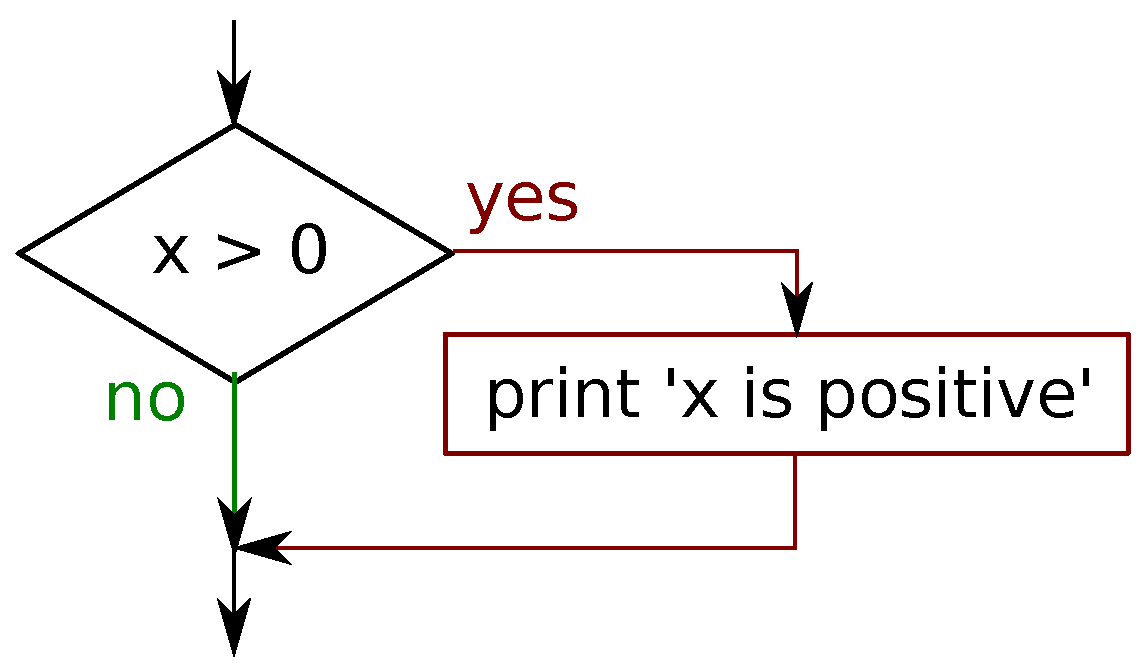
\includegraphics[height=1.75in]{figs2/if.eps}}
\afterfig

If the logical condition is true, then the indented
statement gets executed.  If the logical condition is 
false, the indented statement is skipped.

\index{condition}
\index{compound statement}
\index{statement!compound}

{\tt if} statements have the same structure as function definitions
or {\tt for} loops.  The statement consists of a header line
that ends with the colon character (:) 
followed by an indented block.  Statements like this are
called {\bf compound statements} because they stretch 
across more than one line.

There is no limit on the number of statements that can appear in
the body, but there has to be at least one.
Occasionally, it is useful to have a body with no statements (usually
as a place keeper for code you haven't written yet).  In that
case, you can use the {\tt pass} statement, which does nothing.

\index{pass statement}
\index{statement!pass}

\beforeverb
\begin{verbatim}
if x < 0 :
    pass          # need to handle negative values!
\end{verbatim}
\afterverb
%

\section{Alternative execution}
\label{alternative execution}

\index{alternative execution}
\index{else keyword}
\index{keyword!else}

A second form of the {\tt if} statement is {\bf alternative execution},
in which there are two possibilities and the condition determines
which one gets executed.  The syntax looks like this:

\beforeverb
\begin{verbatim}
if x%2 == 0 :
    print 'x is even'
else :
    print 'x is odd'
\end{verbatim}
\afterverb
%
If the remainder when {\tt x} is divided by 2 is 0, then we
know that {\tt x} is even, and the program displays a message to that
effect.  If the condition is false, the second set of statements is
executed.  

\beforefig
\centerline{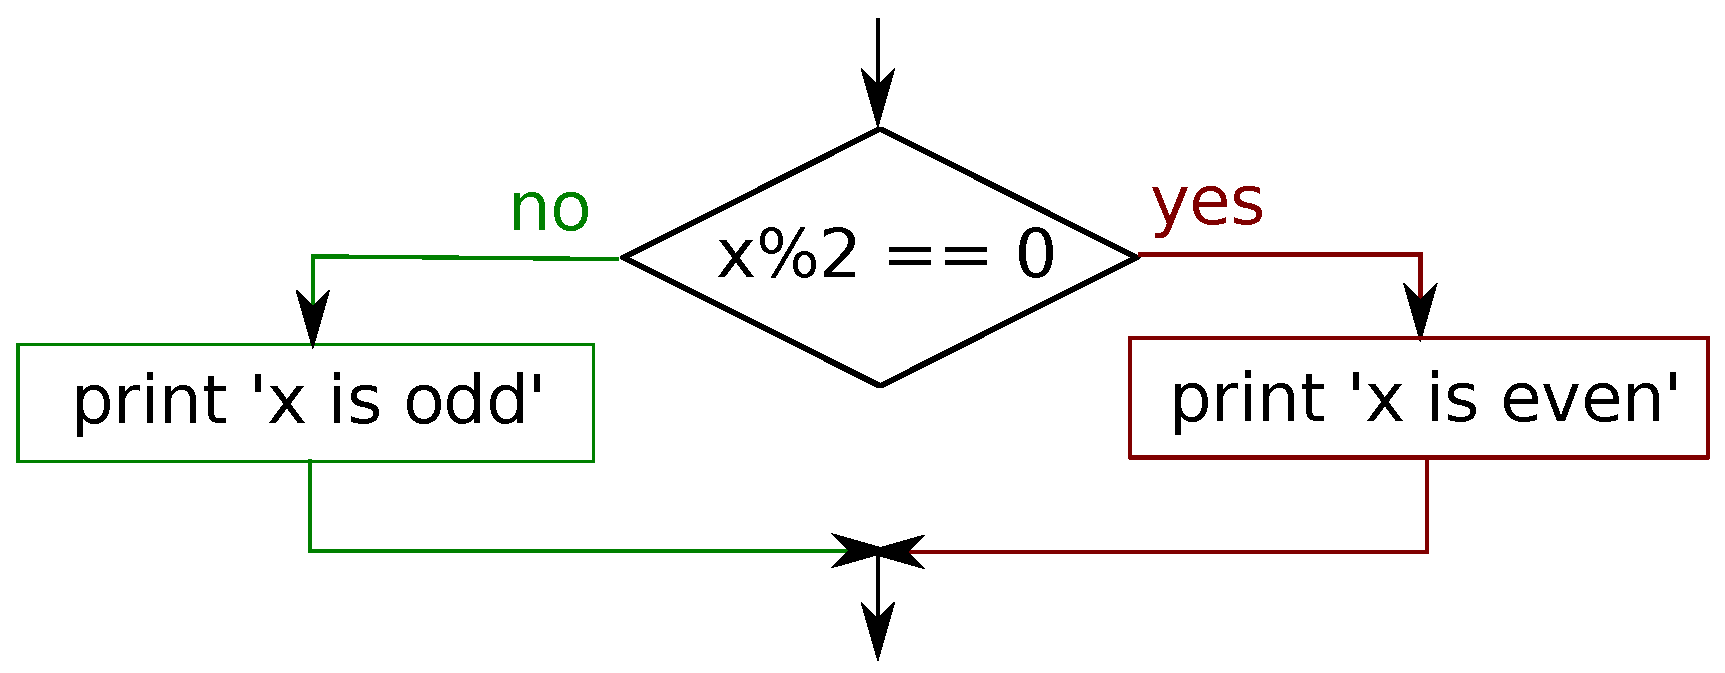
\includegraphics[height=1.75in]{figs2/if-else.eps}}
\afterfig

Since the condition must be true or false, exactly one of
the alternatives will be executed.  The alternatives are called
{\bf branches}, because they are branches in the flow of execution.

\index{branch}



\section{Chained conditionals}
\index{chained conditional}
\index{conditional!chained}

Sometimes there are more than two possibilities and we need more than
two branches.  One way to express a computation like that is a {\bf
chained conditional}:

\beforeverb
\begin{verbatim}
if x < y:
    print 'x is less than y'
elif x > y:
    print 'x is greater than y'
else:
    print 'x and y are equal'
\end{verbatim}
\afterverb
%
{\tt elif} is an abbreviation of ``else if.''  Again, exactly one
branch will be executed.  

\beforefig
\centerline{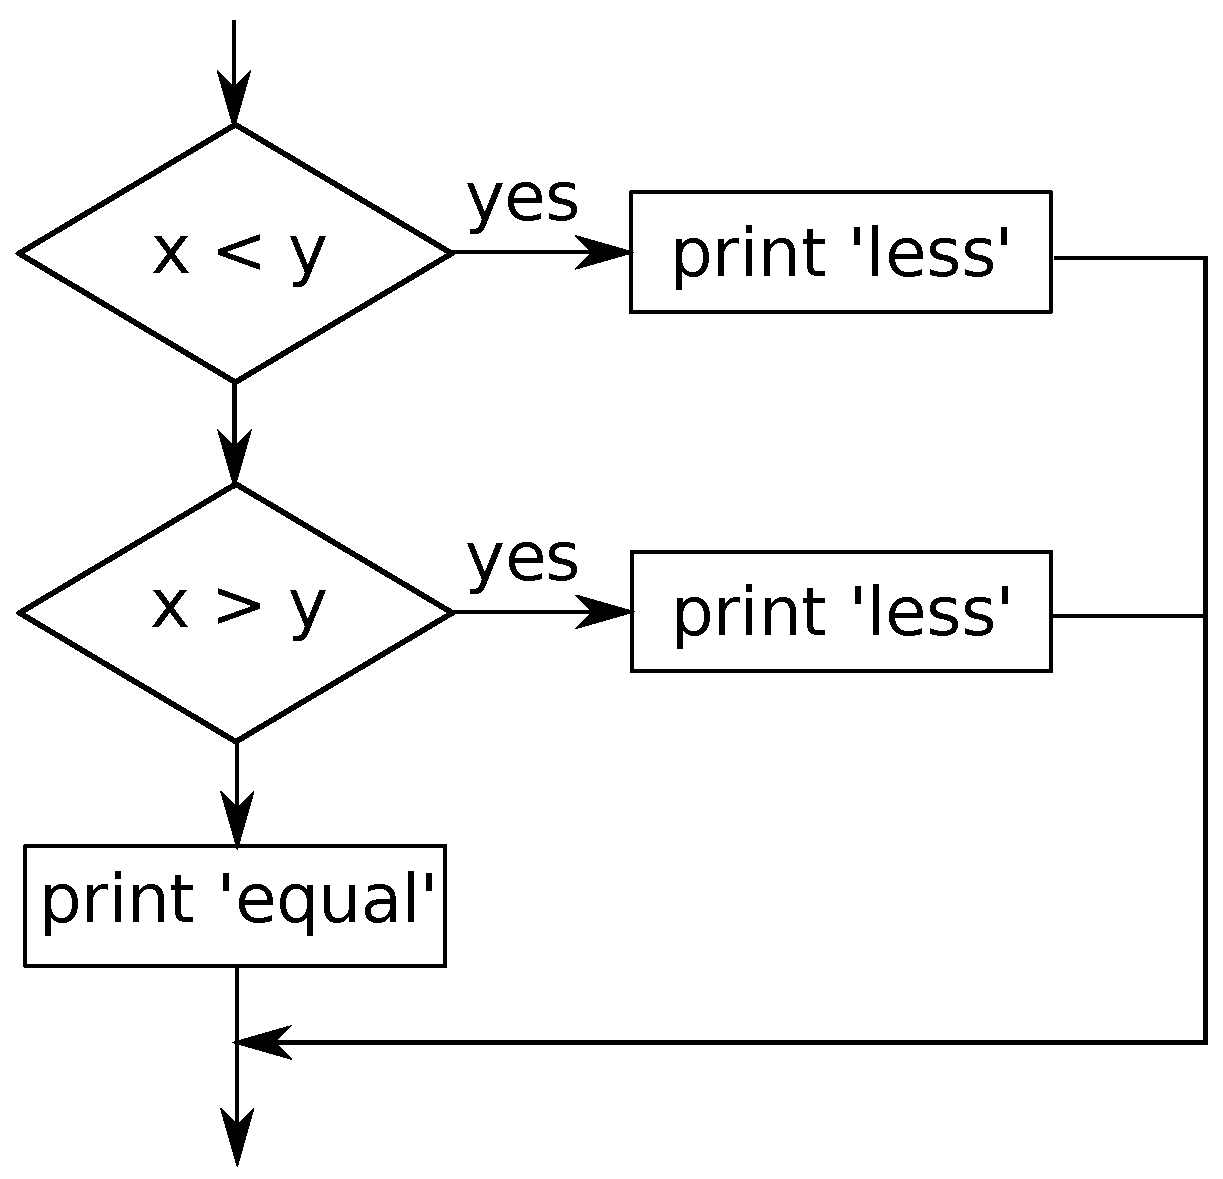
\includegraphics[height=3.00in]{figs2/elif.eps}}
\afterfig

There is no limit on the number of {\tt
elif} statements.  If there is an {\tt else} clause, it has to be
at the end, but there doesn't have to be one.

\index{elif keyword}
\index{keyword!elif}


\beforeverb
\begin{verbatim}
if choice == 'a':
    print 'Bad guess'
elif choice == 'b':
    print 'Good guess'
elif choice == 'c':
    print 'Close, but not correct'
\end{verbatim}
\afterverb
%
Each condition is checked in order.  If the first is false,
the next is checked, and so on.  If one of them is
true, the corresponding branch executes, and the statement
ends.  Even if more than one condition is true, only the
first true branch executes.  


\section{Nested conditionals}
\index{nested conditional}
\index{conditional!nested}

One conditional can also be nested within another.  We could have
written the trichotomy example like this:

\beforeverb
\begin{verbatim}
if x == y:
    print 'x and y are equal'
else:
    if x < y:
        print 'x is less than y'
    else:
        print 'x is greater than y'
\end{verbatim}
\afterverb
%
The outer conditional contains two branches.  The
first branch contains a simple statement.  The second branch
contains another {\tt if} statement, which has two branches of its
own.  Those two branches are both simple statements,
although they could have been conditional statements as well.

\beforefig
\centerline{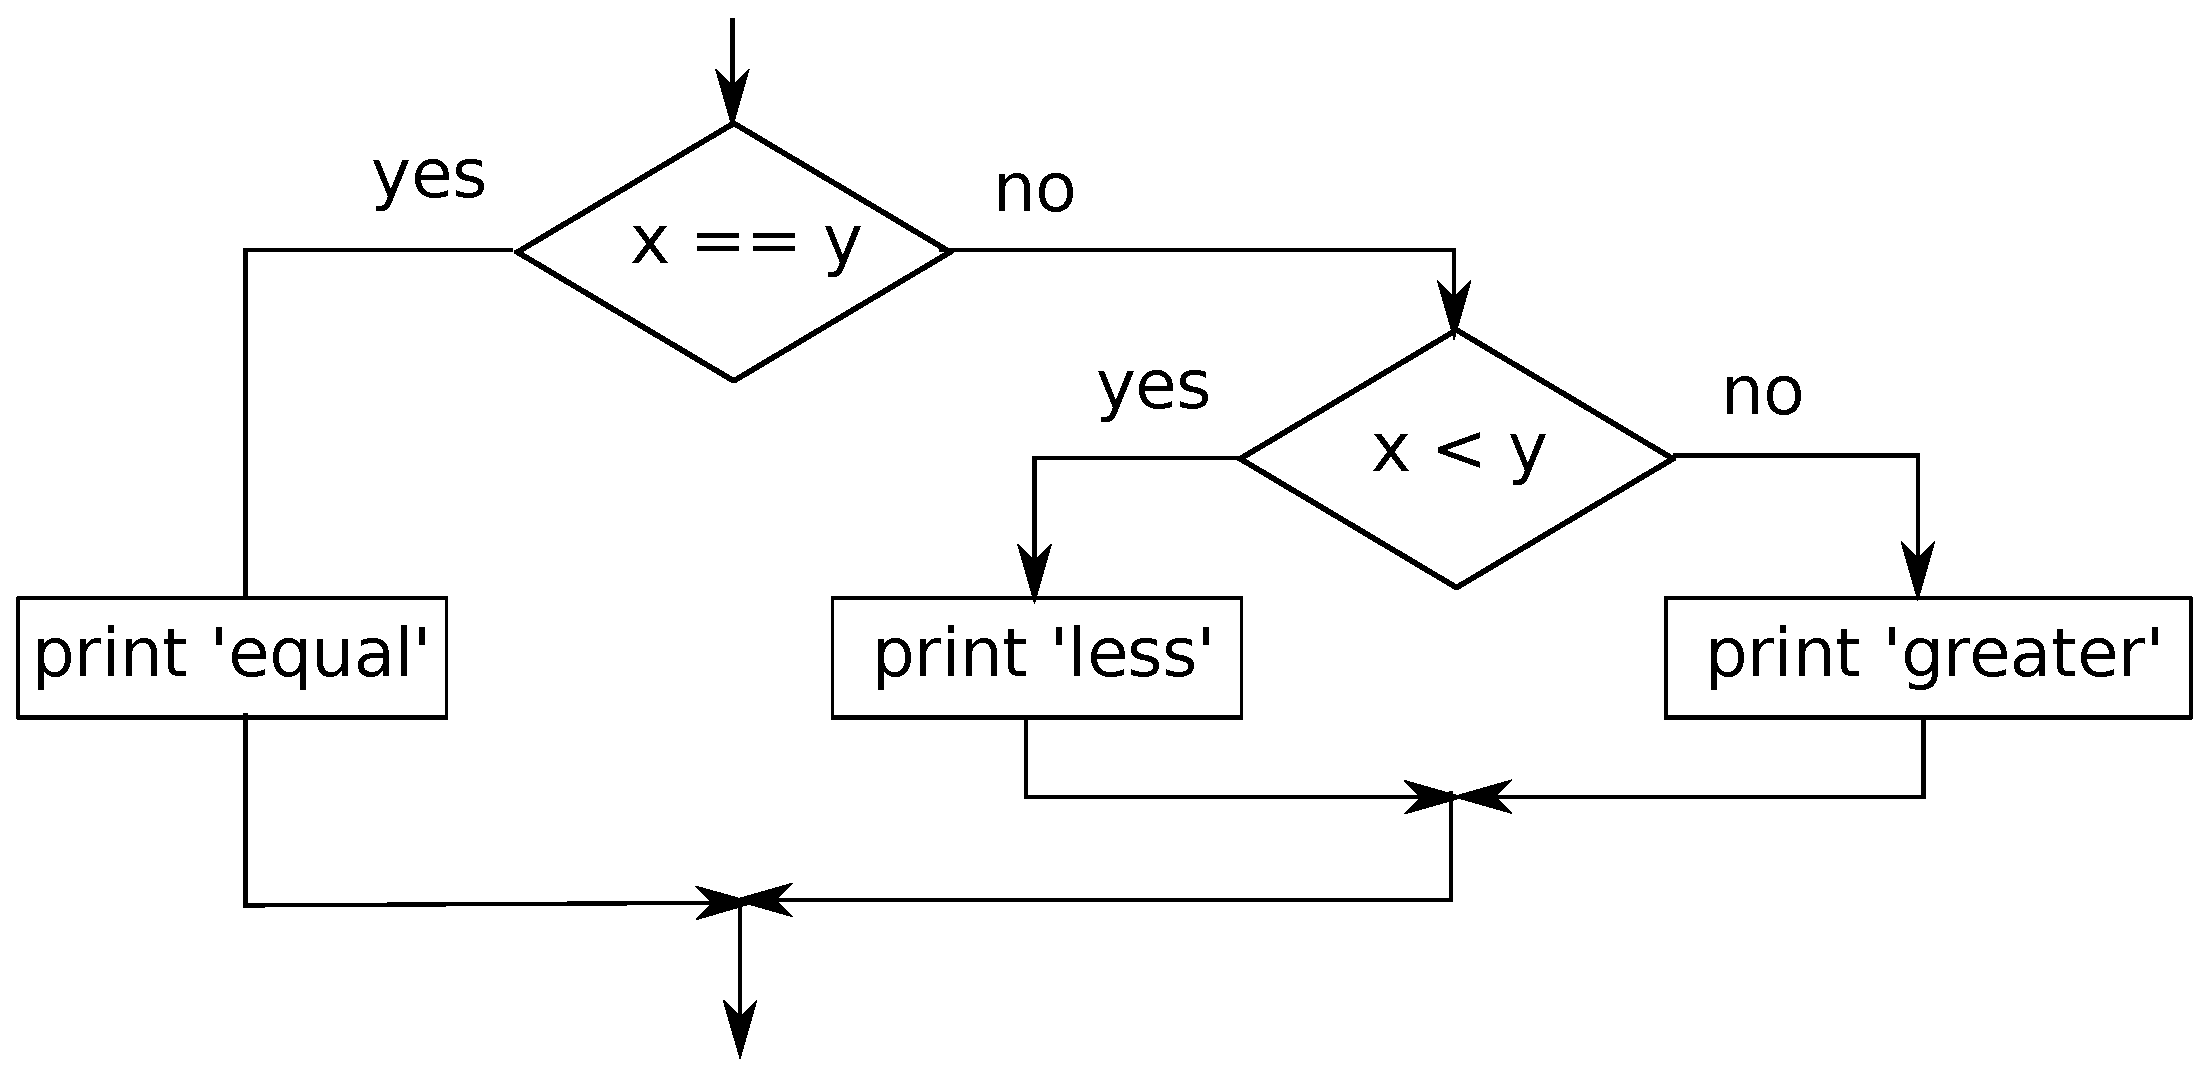
\includegraphics[height=2.50in]{figs2/nested.eps}}
\afterfig

Although the indentation of the statements makes the structure
apparent, {\bf nested conditionals} become difficult to read very
quickly. In general, it is a good idea to avoid them when you can.

Logical operators often provide a way to simplify nested conditional
statements.  For example, we can rewrite the following code using a
single conditional:

\beforeverb
\begin{verbatim}
if 0 < x:
    if x < 10:
        print 'x is a positive single-digit number.'
\end{verbatim}
\afterverb
%
The {\tt print} statement is executed only if we make it past both
conditionals, so we can get the same effect with the {\tt and} operator:

\beforeverb
\begin{verbatim}
if 0 < x and x < 10:
    print 'x is a positive single-digit number.'
\end{verbatim}
\afterverb


\section{Catching exceptions using try and except}
\label{catch1}

Earlier we saw a code segment where we used the \verb"raw_input" and
{\tt int} functions to read and parse an integer number entered by
the user.  We also saw how treacherous doing this could be:

\beforeverb
\begin{verbatim}
>>> speed = raw_input(prompt)
What...is the airspeed velocity of an unladen swallow?
What do you mean, an African or a European swallow?
>>> int(speed)
ValueError: invalid literal for int()
>>>
\end{verbatim}
\afterverb
%
When we are executing these statements in the Python interpreter, 
we get a new prompt from the interpreter, think ``oops'' and move 
on to our next statement.  

However if this code is placed in a 
Python script and this error occurs, your script immediately 
stops in its tracks with a traceback.  
It does not execute the following statement. 
\index{traceback}

Here is a sample program to convert a Fahrenheit temperature 
to a Celsius temperature:
\index{fahrenheit}
\index{celsius}
\index{temperature conversion}

\beforeverb
\begin{verbatim}
inp = raw_input('Enter Fahrenheit Temperature:')
fahr = float(inp)
cel = (fahr - 32.0) * 5.0 / 9.0
print cel
\end{verbatim}
\afterverb
%
If we execute this code and give it invalid input, it simply fails
with an unfriendly error message:

\beforeverb
\begin{verbatim}
python fahren.py 
Enter Fahrenheit Temperature:72
22.2222222222

python fahren.py 
Enter Fahrenheit Temperature:fred
Traceback (most recent call last):
  File "fahren.py", line 2, in <module>
    fahr = float(inp)
ValueError: invalid literal for float(): fred
\end{verbatim}
\afterverb
%
There is a conditional execution structure built into 
Python to handle these types of expected and unexpected
errors called ``try / except''.  The idea of {\tt try}
and {\tt except} is that you know that some sequence
of instruction(s) may have a problem and you want to 
add some statements to be executed if an error occurs.
These extra statements (the except block) are ignored
if there is no error.

You can think of the {\tt try} and {\tt except} feature
in Python as an ``insurance policy'' on a sequence of
statements.

We can rewrite our temperature converter as follows:

\beforeverb
\begin{verbatim}
inp = raw_input('Enter Fahrenheit Temperature:')
try:
    fahr = float(inp)
    cel = (fahr - 32.0) * 5.0 / 9.0
    print cel
except:
    print 'Please enter a number'
\end{verbatim}
\afterverb
%

Python starts by executing the 
sequence of statements in the 
{\tt try} block.  If all goes
well, it skips the {\tt except} block and proceeds.  If an
exception occurs in the {\tt try} block, 
Python jumps out of the {\tt try} block and
executes the sequence of statements in the {\tt except} block.

\beforeverb
\begin{verbatim}
python fahren2.py 
Enter Fahrenheit Temperature:72
22.2222222222

python fahren2.py 
Enter Fahrenheit Temperature:fred
Please enter a number
\end{verbatim}
\afterverb
%

Handling an exception with a {\tt try} statement is called {\bf
catching} an exception.  In this example, the {\tt except} clause
prints an error message.  In general,
catching an exception gives you a chance to fix the problem, or try
again, or at least end the program gracefully.

\section{Short circuit evaluation of logical expressions}
\index{short circuit}

When Python is processing a logical expression such as 
{\tt x >= 2 and (x/y) > 2}, it evaluates the expression
from left-to-right.  Because of the definition of {\tt and},
if {\tt x} is less than 2, the expression {\tt x >= 2} is 
{\tt False} and so the whole expression is {\tt False} regardless
of whether {\tt (x/y) > 2} evaluates to {\tt True} or {\tt False}.

When Python detects that there is nothing to be gained by evaluating
the rest of a logical expression, it stops its evaluation and does
not do the computations in the rest of the logical expression.  
When the evaluation of a logical expression stops because the overall
value is already known, it is called {\bf short-circuiting} 
the evaluation.

\index{guardian pattern}
\index{pattern!guardian}
While this may seem like a fine point, the short circuit behavior
leads to a clever technique called the {\bf guardian pattern}.  
Consider the following code sequence in the Python interpreter:

\beforeverb
\begin{verbatim}
>>> x = 6 
>>> y = 2
>>> x >= 2 and (x/y) > 2
True
>>> x = 1 
>>> y = 0
>>> x >= 2 and (x/y) > 2
False
>>> x = 6
>>> y = 0
>>> x >= 2 and (x/y) > 2
Traceback (most recent call last):
  File "<stdin>", line 1, in <module>
ZeroDivisionError: integer division or modulo by zero
>>> 
\end{verbatim}
\afterverb
%
The third calculation failed because Python was evaluating {\tt (x/y)}
and {\tt y} was zero which causes a runtime error.  But the second example
did \emph{not} fail because the first part of the expression {\tt x >= 2} 
evaluated to {\tt False} so the {\tt (x/y)} was not ever executed 
due to the {\bf short circuit} rule and there was no error.

We can construct the logical expression to strategically place a {\bf guard}
evaluation just before the evaluation that might cause an error as follows:

\beforeverb
\begin{verbatim}
>>> x = 1
>>> y = 0
>>> x >= 2 and y != 0 and (x/y) > 2
False
>>> x = 6 
>>> y = 0
>>> x >= 2 and y != 0 and (x/y) > 2
False
>>> x >= 2 and (x/y) > 2 and y != 0
Traceback (most recent call last):
  File "<stdin>", line 1, in <module>
ZeroDivisionError: integer division or modulo by zero
>>>
\end{verbatim}
\afterverb
%
In the first logical expression, {\tt x >= 2} is {\tt False} so the evaluation
stops at the {\tt and}.  In the second logical expression {\tt x >= 2} is {\tt True}
but {\tt y != 0} is {\tt False} so we never reach {\tt (x/y)}.

In the third logical expression, the {\tt y != 0} is \emph{after} the 
{\tt (x/y) } calculation so the expression fails with an error.

In the second expression, we say that {\tt y != 0} acts as a {\bf guard}
to insure that we only execute {\tt (x/y)} if {\tt y} is non-zero.


\section{Debugging}
\label{whitespace}
\index{debugging}
\index{traceback}

The traceback Python displays when an error occurs contains
a lot of information, but it can be overwhelming, especially
when there are many frames on the stack.  The most
useful parts are usually:

\begin{itemize}

\item What kind of error it was, and

\item Where it occurred.

\end{itemize}

Syntax errors are usually easy to find, but there are a few
gotchas.  Whitespace errors can be tricky because spaces and
tabs are invisible and we are used to ignoring them.

\index{whitespace}

\beforeverb
\begin{verbatim}
>>> x = 5
>>>  y = 6
  File "<stdin>", line 1
    y = 6
    ^
SyntaxError: invalid syntax
\end{verbatim}
\afterverb
%
In this example, the problem is that the second line is indented by
one space.  But the error message points to {\tt y}, which is
misleading.  In general, error messages indicate where the problem was
discovered, but the actual error might be earlier in the code,
sometimes on a previous line.

\index{error!runtime}
\index{runtime error}

The same is true of runtime errors.  Suppose you are trying
to compute a signal-to-noise ratio in decibels.  The formula
is $SNR_{db} = 10 \log_{10} (P_{signal} / P_{noise})$.  In Python,
you might write something like this:

\beforeverb
\begin{verbatim}
import math
signal_power = 9
noise_power = 10
ratio = signal_power / noise_power
decibels = 10 * math.log10(ratio)
print decibels
\end{verbatim}
\afterverb
%
But when you run it, you get an error message\footnote{In Python 3.0,
  you no longer get an error message; the division operator performs
  floating-point division even with integer operands.}:

\index{exception!OverflowError}
\index{OverflowError}

\beforeverb
\begin{verbatim}
Traceback (most recent call last):
  File "snr.py", line 5, in ?
    decibels = 10 * math.log10(ratio)
OverflowError: math range error
\end{verbatim}
\afterverb
%
The error message indicates line 5, but there is nothing
wrong with that line.  To find the real error, it might be
useful to print the value of {\tt ratio}, which turns out to
be 0.  The problem is in line 4, because dividing two integers
does floor division.  The solution is to represent signal power
and noise power with floating-point values.

\index{floor division}
\index{division!floor}

In general, error messages tell you where the problem was discovered, 
but that is often not where it was caused.


\section{Glossary}

\begin{description}

\item[body:] The sequence of statements within a compound statement.
\index{body}

\item[boolean expression:]  An expression whose value is either 
{\tt True} or {\tt False}.
\index{boolean expression}
\index{expression!boolean}

\item[branch:] One of the alternative sequences of statements in
a conditional statement.
\index{branch}

\item[chained conditional:]  A conditional statement with a series
of alternative branches.
\index{chained conditional}
\index{conditional!chained}

\item[comparison operator:] One of the operators that compares
its operands: {\tt ==}, {\tt !=}, {\tt >}, {\tt <}, {\tt >=}, and {\tt <=}.

\item[conditional statement:]  A statement that controls the flow of
execution depending on some condition.
\index{conditional statement}
\index{statement!conditional}

\item[condition:] The boolean expression in a conditional statement
that determines which branch is executed.
\index{condition}

\item[compound statement:]  A statement that consists of a header
and a body.  The header ends with a colon (:).  The body is indented
relative to the header.
\index{compound statement}

\item[guardian pattern:] Where we construct a logical expression 
with additional
comparisons to take advantage of the short circuit behavior.
\index{guardian pattern}
\index{pattern!guardian}

\item[logical operator:] One of the operators that combines boolean
expressions: {\tt and}, {\tt or}, and {\tt not}.

\item[nested conditional:]  A conditional statement that appears
in one of the branches of another conditional statement.
\index{nested conditional}
\index{conditional!nested}

\item[traceback:]  A list of the functions that are executing,
printed when an exception occurs.
\index{traceback}

\item[short circuit:]  When Python is part-way through evaluating a 
logical expression and stops the evaluation because Python 
knows the final value for the expression 
without needing to evaluate the rest of the expression.
\index{short circuit}

\end{description}

\section{Exercises}

\begin{ex}
Rewrite your pay computation to give the employee 1.5 
times the hourly rate for 
hours worked above 40 hours.

\begin{verbatim}
Enter Hours: 45
Enter Rate: 10
Pay: 475.0
\end{verbatim}
\end{ex}

\begin{ex}
Rewrite your pay program using {\tt try} and {\tt except} 
so that your program handles non-numeric input gracefully
by printing a message and exiting the program.
The following shows two executions of the program:

\begin{verbatim}
Enter Hours: 20
Enter Rate: nine
Error, please enter numeric input

Enter Hours: forty
Error, please enter numeric input
\end{verbatim}
\end{ex}

\begin{ex}
Write a program to prompt for a score between 0.0 and 1.0.
If the score is out of range print an error.  If the score
is between 0.0 and 1.0, print a grade using the following 
table:

\begin{verbatim}
Score   Grade
>= 0.9     A
>= 0.8     B
>= 0.7     C
>= 0.6     D
< 0.6    F

Enter score: 0.95
A

Enter score: perfect
Bad score

Enter score: 10.0
Bad score

Enter score: 0.75
C

Enter score: 0.5
F
\end{verbatim}

Run the program repeatedly as shown above to test the 
various different values for input.
\end{ex}

\chapter{Functions}
\label{funcchap}

\section{Function calls}
\label{functionchap}
\index{function call}

In the context of programming, a {\bf function} is a named sequence of
statements that performs a computation.  When you define a function,
you specify the name and the sequence of statements.  Later, you can
``call'' the function by name.  
We have already seen one example of a {\bf function call}:

\beforeverb
\begin{verbatim}
>>> type(32)
<type 'int'>
\end{verbatim}
\afterverb
%
The name of the function is {\tt type}.  The expression in parentheses
is called the {\bf argument} of the function.  The argument is 
a value or variable that we are passing into the function as input 
ot the function.  
The result, for the {\tt type} function, is the type of the argument.

\index{parentheses!argument in}

It is common to say that a function ``takes'' an argument and ``returns''
a result.  The result is called the {\bf return value}.

\index{argument}
\index{return value}

\section{Built-in functions}

Python provides a number of important built-in functions that
we can use without needing to provide the function definition.
In a sense, the creators or Python wrote a set of functions 
to solve common problems and included them in Python for us to use.

The {\tt max} and {\tt min} functions give us the largest and 
smallest values in a list, respectively:

\beforeverb
\begin{verbatim}
>>> max('Hello world')
'w'
>>> min('Hello world')
' '
>>>
\end{verbatim}
\afterverb
%
The {\tt max} function tells us the ``largest character'' in the 
string (which turns out to be the letter ``w'') and the {\tt min}
function shows us the smallest character which turns out to be a 
space.

Another very common built-in function is the {\tt len} function
which tells us how many items are in its argument. If the argument
to {\tt len} is a string, it returns the number of characters 
in the string.

\beforeverb
\begin{verbatim}
>>> len('Hello world')
11
>>>
\end{verbatim}
\afterverb
%
These functions are not limited to looking at strings, they can operate
on any set of values as we will see in later chapters.

\section{Type conversion functions}
\index{conversion!type}
\index{type conversion}

% from Elkner:
% comment on whether these things are _really_ functions?
% use max as an example of a built-in?

% my reply:
% they are on the list of ``built-in functions'' so I am
% willing to call them functions.

Python also provides built-in functions that convert values
from one type to another.  The {\tt int} function takes any value and
converts it to an integer, if it can, or complains otherwise:

\index{int function}
\index{function!int}

\beforeverb
\begin{verbatim}
>>> int('32')
32
>>> int('Hello')
ValueError: invalid literal for int(): Hello
\end{verbatim}
\afterverb
%
{\tt int} can convert floating-point values to integers, but it
doesn't round off; it chops off the fraction part:

\beforeverb
\begin{verbatim}
>>> int(3.99999)
3
>>> int(-2.3)
-2
\end{verbatim}
\afterverb
%
{\tt float} converts integers and strings to floating-point
numbers:

\index{float function}
\index{function!float}

\beforeverb
\begin{verbatim}
>>> float(32)
32.0
>>> float('3.14159')
3.14159
\end{verbatim}
\afterverb
%
Finally, {\tt str} converts its argument to a string:

\index{str function}
\index{function!str}

\beforeverb
\begin{verbatim}
>>> str(32)
'32'
>>> str(3.14159)
'3.14159'
\end{verbatim}
\afterverb
%

\section{Random numbers}

\index{random number}
\index{number, random}
\index{deterministic}
\index{pseudorandom}

Given the same inputs, most computer programs generate the same
outputs every time, so they are said to be {\bf deterministic}.
Determinism is usually a good thing, since we expect the same
calculation to yield the same result.  For some applications, though,
we want the computer to be unpredictable.  Games are an obvious
example, but there are more.

Making a program truly nondeterministic turns out to be not so easy,
but there are ways to make it at least seem nondeterministic.  One of
them is to use {\bf algorithms} that generate {\bf pseudorandom} numbers.
Pseudorandom numbers are not truly random because they are generated
by a deterministic computation, but just by looking at the numbers it
is all but impossible to distinguish them from random.

\index{random module}
\index{module!random}

The {\tt random} module provides functions that generate
pseudorandom numbers (which I will simply call ``random'' from
here on).

\index{random function}
\index{function!random}

The function {\tt random} returns a random float
between 0.0 and 1.0 (including 0.0 but not 1.0).  Each time you
call {\tt random}, you get the next number in a long series.  To see a
sample, run this loop:

\beforeverb
\begin{verbatim}
import random

for i in range(10):
    x = random.random()
    print x
\end{verbatim}
\afterverb
%
This program produces the following list of 10 random numbers
between 0.0 and up to but not including 1.0.
\beforeverb
\begin{verbatim}
0.301927091705
0.513787075867
0.319470430881
0.285145917252
0.839069045123
0.322027080731
0.550722110248
0.366591677812
0.396981483964
0.838116437404
\end{verbatim}
\afterverb
%
\begin{ex}
Run the program on your system and see what numbers you get.
Run the program more than once and see what numbers you get.
\end{ex}

The {\tt random} function is only one of many 
functions which handle random numbers.
The function {\tt randint} takes parameters {\tt low} and
{\tt high} and returns an integer between {\tt low} and
{\tt high} (including both).

\index{randint function}
\index{function!randint}

\beforeverb
\begin{verbatim}
>>> random.randint(5, 10)
5
>>> random.randint(5, 10)
9
\end{verbatim}
\afterverb
%
To choose an element from a sequence at random, you can use
{\tt choice}:

\index{choice function}
\index{function!choice}

\beforeverb
\begin{verbatim}
>>> t = [1, 2, 3]
>>> random.choice(t)
2
>>> random.choice(t)
3
\end{verbatim}
\afterverb
%
The {\tt random} module also provides functions to generate
random values from continuous distributions including
Gaussian, exponential, gamma, and a few more.

\section{Math functions}
\index{math function}
\index{function, math}

Python has a math {\bf module} that provides most of the familiar
mathematical functions.  
Before we can use the module, we have to import it:

\index{module}
\index{module object}
\beforeverb
\begin{verbatim}
>>> import math
\end{verbatim}
\afterverb
%
This statement creates a {\bf module object} named math.  If
you print the module object, you get some information about it:

\beforeverb
\begin{verbatim}
>>> print math
<module 'math' from '/usr/lib/python2.5/lib-dynload/math.so'>
\end{verbatim}
\afterverb
%
The module object contains the functions and variables defined in the
module.  To access one of the functions, you have to specify the name
of the module and the name of the function, separated by a dot (also
known as a period).  This format is called {\bf dot notation}.

\index{dot notation}

\beforeverb
\begin{verbatim}
>>> ratio = signal_power / noise_power
>>> decibels = 10 * math.log10(ratio)

>>> radians = 0.7
>>> height = math.sin(radians)
\end{verbatim}
\afterverb
%
The first example computes the logarithm base 10 of the
signal-to-noise ratio.  The math module also provides a
function called {\tt log} that computes logarithms base {\tt e}.

\index{log function}
\index{function!log}
\index{sine function}
\index{radian}
\index{trigonometric function}
\index{function, trigonometric}

The second example finds the sine of {\tt radians}.  The name of the
variable is a hint that {\tt sin} and the other trigonometric
functions ({\tt cos}, {\tt tan}, etc.)  take arguments in radians. To
convert from degrees to radians, divide by 360 and multiply by $2
\pi$:

\beforeverb
\begin{verbatim}
>>> degrees = 45
>>> radians = degrees / 360.0 * 2 * math.pi
>>> math.sin(radians)
0.707106781187
\end{verbatim}
\afterverb
%
The expression {\tt math.pi} gets the variable {\tt pi} from the math
module.  The value of this variable is an approximation
of $\pi$, accurate to about 15 digits.

\index{pi}

If you know
your trigonometry, you can check the previous result by comparing it to
the square root of two divided by two:

\index{sqrt function}
\index{function!sqrt}

\beforeverb
\begin{verbatim}
>>> math.sqrt(2) / 2.0
0.707106781187
\end{verbatim}
\afterverb
%


\section{Adding new functions}

So far, we have only been using the functions that come with Python,
but it is also possible to add new functions.
A {\bf function definition} specifies the name of a new function and
the sequence of statements that execute when the function is called.
Once we define a function, we can reuse the function over and over 
throughout our program.

\index{function}
\index{function definition}
\index{definition!function}

Here is an example:

\beforeverb
\begin{verbatim}
def print_lyrics():
    print "I'm a lumberjack, and I'm okay."
    print 'I sleep all night and I work all day.'
\end{verbatim}
\afterverb
%
{\tt def} is a keyword that indicates that this is a function
definition.  The name of the function is \verb"print_lyrics".  The
rules for function names are the same as for variable names: letters,
numbers and some punctuation marks are legal, but the first character
can't be a number.  You can't use a keyword as the name of a function,
and you should avoid having a variable and a function with the same
name.

\index{def keyword}
\index{keyword!def}
\index{argument}

The empty parentheses after the name indicate that this function
doesn't take any arguments.   Later we will build functions that 
take arguments as their inputs.

\index{parentheses!empty}
\index{header}
\index{body}
\index{indentation}
\index{colon}

The first line of the function definition is called the {\bf header};
the rest is called the {\bf body}.  The header has to end with a colon
and the body has to be indented.  By convention, the indentation is
always four spaces (see Section~\ref{editor}).  The body can contain
any number of statements.

The strings in the print statements are enclosed in double
quotes.  Single quotes and double quotes do the same thing;
most people use single quotes except in cases like this where
a single quote (which is also an apostrophe) appears in the string.

\index{ellipses}

If you type a function definition in interactive mode, the interpreter
prints ellipses (\emph{...}) to let you know that the definition
isn't complete:

\beforeverb
\begin{verbatim}
>>> def print_lyrics():
...     print "I'm a lumberjack, and I'm okay."
...     print 'I sleep all night and I work all day.'
...
\end{verbatim}
\afterverb
%
To end the function, you have to enter an empty line (this is
not necessary in a script).

Defining a function creates a variable with the same name.

\beforeverb
\begin{verbatim}
>>> print print_lyrics
<function print_lyrics at 0xb7e99e9c>
>>> print type(print_lyrics)
<type 'function'>
\end{verbatim}
\afterverb
%
The value of \verb"print_lyrics" is a {\bf function object}, which
has type \verb"'function'".

\index{function object}
\index{object!function}

The syntax for calling the new function is the same as
for built-in functions:

\beforeverb
\begin{verbatim}
>>> print_lyrics()
I'm a lumberjack, and I'm okay.
I sleep all night and I work all day.
\end{verbatim}
\afterverb
%
Once you have defined a function, you can use it inside another
function.  For example, to repeat the previous refrain, we could write
a function called \verb"repeat_lyrics":

\beforeverb
\begin{verbatim}
def repeat_lyrics():
    print_lyrics()
    print_lyrics()
\end{verbatim}
\afterverb
%
And then call \verb"repeat_lyrics":

\beforeverb
\begin{verbatim}
>>> repeat_lyrics()
I'm a lumberjack, and I'm okay.
I sleep all night and I work all day.
I'm a lumberjack, and I'm okay.
I sleep all night and I work all day.
\end{verbatim}
\afterverb
%
But that's not really how the song goes.


\section{Definitions and uses}
\index{function definition}

Pulling together the code fragments from the previous section, the
whole program looks like this:

\beforeverb
\begin{verbatim}
def print_lyrics():
    print "I'm a lumberjack, and I'm okay."
    print 'I sleep all night and I work all day.'

def repeat_lyrics():
    print_lyrics()
    print_lyrics()

repeat_lyrics()
\end{verbatim}
\afterverb
%
This program contains two function definitions: \verb"print_lyrics" and
\verb"repeat_lyrics".  Function definitions get executed just like other
statements, but the effect is to create function objects.  The statements
inside the function do not get executed until the function is called, and
the function definition generates no output.

\index{use before def}

As you might expect, you have to create a function before you can
execute it.  In other words, the function definition has to be
executed before the first time it is called.

\begin{ex}
Move the last line of this program
to the top, so the function call appears before the definitions. Run 
the program and see what error
message you get.
\end{ex}

\begin{ex}
Move the function call back to the bottom
and move the definition of \verb"print_lyrics" after the definition of
\verb"repeat_lyrics".  What happens when you run this program?
\end{ex}


\section{Flow of execution}
\index{flow of execution}

In order to ensure that a function is defined before its first use,
you have to know the order in which statements are executed, which is
called the {\bf flow of execution}.

Execution always begins at the first statement of the program.
Statements are executed one at a time, in order from top to bottom.

Function \emph{definitions} do not alter the flow of execution of the
program, but remember that statements inside the function are not
executed until the function is called.

A function call is like a detour in the flow of execution. Instead of
going to the next statement, the flow jumps to the body of
the function, executes all the statements there, and then comes back
to pick up where it left off.

That sounds simple enough, until you remember that one function can
call another.  While in the middle of one function, the program might
have to execute the statements in another function. But while
executing that new function, the program might have to execute yet
another function!

Fortunately, Python is good at keeping track of where it is, so each
time a function completes, the program picks up where it left off in
the function that called it.  When it gets to the end of the program,
it terminates.

What's the moral of this sordid tale?  When you read a program, you
don't always want to read from top to bottom.  Sometimes it makes
more sense if you follow the flow of execution.


\section{Parameters and arguments}
\label{parameters}
\index{parameter}
\index{function parameter}
\index{argument}
\index{function argument}

Some of the built-in functions we have seen require arguments.  For
example, when you call {\tt math.sin} you pass a number
as an argument.  Some functions take more than one argument:
{\tt math.pow} takes two, the base and the exponent.

Inside the function, the arguments are assigned to
variables called {\bf parameters}.  Here is an example of a
user-defined function that takes an argument:

\index{parentheses!parameters in}

\beforeverb
\begin{verbatim}
def print_twice(bruce):
    print bruce
    print bruce
\end{verbatim}
\afterverb
%
This function assigns the argument to a parameter
named {\tt bruce}.  When the function is called, it prints the value of
the parameter (whatever it is) twice.

This function works with any value that can be printed.

\beforeverb
\begin{verbatim}
>>> print_twice('Spam')
Spam
Spam
>>> print_twice(17)
17
17
>>> print_twice(math.pi)
3.14159265359
3.14159265359
\end{verbatim}
\afterverb
%
The same rules of composition that apply to built-in functions also
apply to user-defined functions, so we can use any kind of expression
as an argument for \verb"print_twice":

\index{composition}

\beforeverb
\begin{verbatim}
>>> print_twice('Spam '*4)
Spam Spam Spam Spam
Spam Spam Spam Spam
>>> print_twice(math.cos(math.pi))
-1.0
-1.0
\end{verbatim}
\afterverb
%
The argument is evaluated before the function is called, so
in the examples the expressions \verb"'Spam '*4" and
{\tt math.cos(math.pi)} are only evaluated once.

\index{argument}

You can also use a variable as an argument:

\beforeverb
\begin{verbatim}
>>> michael = 'Eric, the half a bee.'
>>> print_twice(michael)
Eric, the half a bee.
Eric, the half a bee.
\end{verbatim}
\afterverb
%
The name of the variable we pass as an argument ({\tt michael}) has
nothing to do with the name of the parameter ({\tt bruce}).  It
doesn't matter what the value was called back home (in the caller);
here in \verb"print_twice", we call everybody {\tt bruce}.

\section{Fruitful functions and void functions}

\index{fruitful function}
\index{void function}
\index{function, fruitful}
\index{function, void} 

Some of the functions we are using, such as the math functions, yield
results; for lack of a better name, I call them {\bf fruitful
  functions}.  Other functions, like \verb"print_twice", perform an
action but don't return a value.  They are called {\bf void
  functions}.

When you call a fruitful function, you almost always
want to do something with the result; for example, you might
assign it to a variable or use it as part of an expression:

\beforeverb
\begin{verbatim}
x = math.cos(radians)
golden = (math.sqrt(5) + 1) / 2
\end{verbatim}
\afterverb
%
When you call a function in interactive mode, Python displays
the result:

\beforeverb
\begin{verbatim}
>>> math.sqrt(5)
2.2360679774997898
\end{verbatim}
\afterverb
%
But in a script, if you call a fruitful function and do 
not store the result of the function in a variable,
the return value vanishes into the mist!

\beforeverb
\begin{verbatim}
math.sqrt(5)
\end{verbatim}
\afterverb
%
This script computes the square root of 5, but since it doesn't store
the result in a variable or display the result, it is not very useful.

\index{interactive mode}
\index{script mode}

Void functions might display something on the screen or have some
other effect, but they don't have a return value.  If you try to
assign the result to a variable, you get a special value called
{\tt None}.

\index{None special value}
\index{special value!None}

\beforeverb
\begin{verbatim}
>>> result = print_twice('Bing')
Bing
Bing
>>> print result
None
\end{verbatim}
\afterverb
%
The value {\tt None} is not the same as the string \verb"'None'". 
It is a special value that has its own type:

\beforeverb
\begin{verbatim}
>>> print type(None)
<type 'NoneType'>
\end{verbatim}
\afterverb
%
To return a result from a function, we use the {\tt return} statement 
in our function.  For example, we could make a very 
simple function called {\tt addtwo}
that adds two numbers together and return a result.

\beforeverb
\begin{verbatim}
def addtwo(a, b):
    added = a + b
    return added

x = addtwo(3, 5)
print x
\end{verbatim}
\afterverb
%
When this script executes, the {\tt print} statement will print out ``8''
because the {\tt addtwo} function was called with 3 and 5 as arguments.
Within the function the parameters {\tt a} and {\tt b} were 3 and 5 
respectively. The function computed the sum of the two numbers and placed
it in the local function variable named {\tt added} 
and used the {\tt return} statement 
to send the computed value back to the calling code 
as the function result which was assigned
to the variable {\tt x} and printed out.


\section{Why functions?}
\index{function, reasons for}

It may not be clear why it is worth the trouble to divide
a program into functions.  There are several reasons:

\begin{itemize}

\item Creating a new function gives you an opportunity to name a group
of statements, which makes your program easier to read, understand 
and debug.

\item Functions can make a program smaller by eliminating repetitive
code.  Later, if you make a change, you only have
to make it in one place.

\item Dividing a long program into functions allows you to debug the
parts one at a time and then assemble them into a working whole.

\item Well-designed functions are often useful for many programs.
Once you write and debug one, you can reuse it.

\end{itemize}

Throughout the rest of the book, often we will use a function definition to 
explain a concept.  Part of the skill of creating and using functions is
to have a function properly capture an idea such as ``find the smallest
value in a list of values''.  Later we will show you code that finds
the smallest in a list of values and we will present it to you as a function
named {\tt min} which takes a list of values as its argument and 
returns the smallest value in the list.


\section{Debugging}
\label{editor}
\index{debugging}

If you are using a text editor to write your scripts, you might
run into problems with spaces and tabs.  The best way to avoid
these problems is to use spaces exclusively (no tabs).  Most text
editors that know about Python do this by default, but some
don't.

\index{whitespace}

Tabs and spaces are usually invisible, which makes them
hard to debug, so try to find an editor that manages indentation
for you.

Also, don't forget to save your program before you run it.  Some
development environments do this automatically, but some don't.
In that case the program you are looking at in the text editor
is not the same as the program you are running.

Debugging can take a long time if you keep running the same,
incorrect, program over and over!

Make sure that the code you are looking at is the code you are running.
If you're not sure, put something like \verb"print 'hello'" at the
beginning of the program and run it again.  If you don't see
\verb"hello", you're not running the right program!




\section{Glossary}

\begin{description}

\item[algorithm:]  A general process for solving a category of
problems.
\index{algorithm}

\item[argument:]  A value provided to a function when the function is called.
This value is assigned to the corresponding parameter in the function.
\index{argument}

\item[body:] The sequence of statements inside a function definition.
\index{body}

\item[composition:] Using an expression as part of a larger expression,
or a statement as part of a larger statement.
\index{composition}

\item[deterministic:] Pertaining to a program that does the same
thing each time it runs, given the same inputs.
\index{deterministic}

\item[dot notation:]  The syntax for calling a function in another
module by specifying the module name followed by a dot (period) and
the function name.
\index{dot notation}

\item[flow of execution:]  The order in which statements are executed during
a program run.
\index{flow of execution}

\item[fruitful function:] A function that returns a value.
\index{fruitful function}

\item[function:] A named sequence of statements that performs some
useful operation.  Functions may or may not take arguments and may or
may not produce a result.
\index{function}

\item[function call:] A statement that executes a function. It
consists of the function name followed by an argument list.
\index{function call}

\item[function definition:]  A statement that creates a new function,
specifying its name, parameters, and the statements it executes.
\index{function definition}

\item[function object:]  A value created by a function definition.
The name of the function is a variable that refers to a function
object.
\index{function definition}

\item[header:] The first line of a function definition.
\index{header}

\item[import statement:] A statement that reads a module file and creates
a module object.
\index{import statement}
\index{statement!import}

\item[module object:] A value created by an {\tt import} statement
that provides access to the data and code defined in a module.
\index{module}

\item[parameter:] A name used inside a function to refer to the value
passed as an argument.
\index{parameter}

\item[pseudorandom:] Pertaining to a sequence of numbers that appear
to be random, but are generated by a deterministic program.
\index{pseudorandom}

\item[return value:]  The result of a function.  If a function call
is used as an expression, the return value is the value of
the expression.
\index{return value}

\item[void function:] A function that doesn't return a value.
\index{void function}


\end{description}


\section{Exercises}

\begin{ex}
Rewrite your pay computation with time-and-a-half for overtime
and create a function called {\tt computepay} which takes
two parameters ({\tt hours} and {\tt rate}).

\begin{verbatim}
Enter Hours: 45
Enter Rate: 10
Pay: 475.0
\end{verbatim}
\end{ex}

\begin{ex}
Rewrite the grade program from the previous chapter 
using a function called {\tt computegrade} that takes
a score as its parameter and returns a grade as a string.

\begin{verbatim}
Score   Grade
> 0.9     A
> 0.8     B
> 0.7     C
> 0.6     D
<= 0.6    F

Program Execution:

Enter score: 0.95
A

Enter score: perfect
Bad score

Enter score: 10.0
Bad score

Enter score: 0.75
C

Enter score: 0.5
F
\end{verbatim}

Run the program repeatedly to test the various different values
for input.
\end{ex}




\chapter{Iteration}
\index{iteration}


\section{Updating variables}
\label{update}

\index{update}
\index{variable!updating}

A common pattern in assignment statements is an assignment statement
that updates a variable - 
where the new value of the variable depends on the old.

\beforeverb
\begin{verbatim}
x = x+1
\end{verbatim}
\afterverb
%
This means ``get the current value of {\tt x}, add one, and then
update {\tt x} with the new value.''

If you try to update a variable that doesn't exist, you get an
error, because Python evaluates the right side before it assigns
a value to {\tt x}:

\beforeverb
\begin{verbatim}
>>> x = x+1
NameError: name 'x' is not defined
\end{verbatim}
\afterverb
%
Before you can update a variable, you have to {\bf initialize}
it, usually with a simple assignment:

\index{initialization (before update)}

\beforeverb
\begin{verbatim}
>>> x = 0
>>> x = x+1
\end{verbatim}
\afterverb
%
Updating a variable by adding 1 is called an {\bf increment};
subtracting 1 is called a {\bf decrement}.

\index{increment}
\index{decrement}

\section{The {\tt while} statement}

\index{statement!while}
\index{while loop}
\index{loop!while}
\index{iteration}

Computers are often used to automate repetitive tasks.  Repeating
identical or similar tasks without making errors is something that
computers do well and people do poorly.
Because iteration is so common, Python provides several
language features to make it easier.  

One form of iteration in Python is the {\tt while} statement.  Here is 
a simple program that counts down from five and then says ``Blastoff!''.

\beforeverb
\begin{verbatim}
n = 5
while n > 0:
    print n
    n = n-1
print 'Blastoff!'
\end{verbatim}
\afterverb
%
You can almost read the {\tt while} statement as if it were English.
It means, ``While {\tt n} is greater than 0,
display the value of {\tt n} and then reduce the value of
{\tt n} by 1.  When you get to 0, exit the while statement and
display the word {\tt Blastoff!}''

\index{flow of execution}

More formally, here is the flow of execution for a {\tt while} statement:

\begin{enumerate}

\item Evaluate the condition, yielding {\tt True} or {\tt False}.

\item If the condition is false, exit the {\tt while} statement
and continue execution at the next statement.

\item If the condition is true, execute the
body and then go back to step 1.

\end{enumerate}

This type of flow is called a {\bf loop} because the third step
loops back around to the top.  Each time we execute the body of 
the loop, we call it an {\bf iteration}.  For the above loop, we 
would say, ``It had five iterations'' which means that the body of
of the loop was executed five times.

\index{condition}
\index{loop}
\index{body}

The body of the loop should change the value of one or more variables
so that eventually the condition becomes false and the loop
terminates.  
We call the variable that changes each time the loop
executes and controls when the loop finishes the 
{\bf iteration variable}.
If there is no iteration variable, the loop will repeat forever, 
resulting in an {\bf infinite loop}.  

\section{Infinite loops}

An endless source of amusement for 
programmers is the observation that the directions on shampoo,
``Lather, rinse, repeat,'' are an infinite loop because 
there is no {\bf iteration variable} telling you how many times
to execute the loop.

\index{infinite loop}
\index{loop!infinite}

In the case of {\tt countdown}, we can prove that the loop
terminates because we know that the value of {\tt n} is finite, and we
can see that the value of {\tt n} gets smaller each time through the
loop, so eventually we have to get to 0.  Other times a loop is obviously
infinite because it has no iteration variable at all.

In other cases, it is not so easy to tell.  The code below defines a function
that takes an positive number as its parameter and computes a different 
kind of sequence.
Remember that the percent sign is the {\bf modulo} operator which gives us the
remainder if a division were performed.

\beforeverb
\begin{verbatim}
def sequence(n):
    while n != 1:
        print n,            # Use comma to suppress newline
        if n%2 == 0:        # n is even
            n = n/2
        else:               # n is odd
            n = n*3+1
\end{verbatim}
\afterverb
%
The condition for this loop is {\tt n != 1}\footnote{Remember that {\tt != } is the operator for 'not equal'.}, 
so the loop will continue
until {\tt n} is {\tt 1}, which makes the condition false.

Each time through the loop, the program outputs the value of {\tt n}
and then checks whether it is even or odd.  If it is even, {\tt n} is 
divided by 2.  If it is odd, the value of {\tt n} is replaced with
{\tt n*3+1}. For example, if the argument passed
to {\tt sequence} is 3, the resulting sequence is 3, 10, 5, 16, 8, 4, 2.

Since {\tt n} sometimes increases and sometimes decreases, there is no
obvious proof that {\tt n} will ever reach 1, or that the program
terminates.  For some particular values of {\tt n}, we can prove
termination.  For example, if the starting value is a power of two,
then the value of {\tt n} will be even each time through the loop
until it reaches 1. The previous example ends with such a sequence,
starting with 16.

\beforeverb
\begin{verbatim}
>>> def sequence(n):
...     while n != 1:
...         print n,
...         if n%2 == 0:        # n is even
...             n = n/2
...         else:               # n is odd
...             n = n*3+1
... 
>>> sequence(3)
3 10 5 16 8 4 2
>>> sequence(16)
16 8 4 2
>>> sequence(50)
50 25 76 38 19 58 29 88 44 22 11 34 17 52 26 13 40 20 10 5 16 8 4 2
\end{verbatim}
\afterverb
%
You can try this sequence with a variety of integer or floating 
point numbers as the argument.  
Since the main loop repeatedly divides a number
by two, an argument in the billions converges to one in 
relatively few steps.  
It is more fun to try floating point arguments 
such as 12.45 as it takes more iterations before the sequence
converges to one.

\index{Collatz conjecture}
The hard question is whether we can prove that this program terminates
for \emph{all positive values} of {\tt n}.  So far\footnote{See
  \url{wikipedia.org/wiki/Collatz_conjecture}.}, no one has
been able to prove it \emph{or} disprove it!

\section{``Infinite loops'' and {\tt break}}
\index{break statement}
\index{statement!break}

Sometimes you don't know it's time to end a loop until you get half
way through the body.  In that case you can write an infinite loop on purpose
and then use the {\tt break} statement to jump out of the loop.

This loop is obviously an {\bf infinite loop} because the logical 
expression on the
{\tt while} statement is simply the logical constant {\tt True}:
\beforeverb
\begin{verbatim}
n = 10
while True:
    print n, 
    n = n - 1
print 'Done!'
\end{verbatim}
\afterverb
%
If you make the mistake and run this code, you will learn quickly how
to stop a runaway Python process on your system or find where the power-off
button is on your computer.  
This program will 
run forever or until your battery runs out 
because the logical expression at the top of the loop 
is always true by virtue of the fact that the expression is the 
constant value {\tt True}.

While this is a dysfunctional infinite loop, we can still use this pattern
to build useful loops as long as we carefully add code to the 
body of the loop to explicitly exit the loop using {\tt break} 
when we have reached 
the exit condition.

For example, suppose you want to take input from the user until they
type {\tt done}.  You could write:

\beforeverb
\begin{verbatim}
while True:
    line = raw_input('> ')
    if line == 'done':
        break
    print line
print 'Done!'
\end{verbatim}
\afterverb
%
The loop condition is {\tt True}, which is always true, so the
loop runs repeatedly until it hits the break statement.

Each time through, it prompts the user with an angle bracket.
If the user types {\tt done}, the {\tt break} statement exits
the loop.  Otherwise the program echoes whatever the user types
and goes back to the top of the loop.  Here's a sample run:

\beforeverb
\begin{verbatim}
> hello there
hello there
> finished
finished
> done
Done!
\end{verbatim}
\afterverb
%
This way of writing {\tt while} loops is common because you
can check the condition anywhere in the loop (not just at the
top) and you can express the stop condition affirmatively
(``stop when this happens'') rather than negatively (``keep going
until that happens.'').

\section{Finishing iterations with {\tt continue}}
\index{continue statement}
\index{statement!continue}

Sometimes you are in an iteration of a loop and want to finish the
current iteration and immediately jump to the next iteration.
In that case you can use the {\tt continue}
statement to skip to the next iteration without finishing the
body of the loop for the current iteration.

Here is an example of a loop that copies its input until the user
types ``done'', but treats lines that start with the hash character
as lines not to be printed (kind of like Python comments).

\beforeverb
\begin{verbatim}
while True:
    line = raw_input('> ')
    if line[0] == '#' :
        continue
    if line == 'done':
        break
    print line
print 'Done!'
\end{verbatim}
\afterverb
%
Here is a sample run of this new program with {\tt continue} added.

\beforeverb
\begin{verbatim}
> hello there
hello there
> # don't print this
> print this!
print this!
> done
Done!
\end{verbatim}
\afterverb
%
All the lines are printed except the one that starts with the hash
sign because when the {\tt continue} is executed, it ends 
the current iteration and jumps
back to the {\tt while} statement to start the next iteration, thus 
skipping the {\tt print} statement.

\section{Definite loops using {\tt for} }
\index{for statement}
\index{statement!for}

Sometimes we want to loop through a {\bf set} of things such 
as a list of words, the lines in a file or a list of numbers.
When we have a list of things to loop through, we can
construct a \emph{definite} loop using a {\tt for} statement.
We call the {\tt while} statement an \emph{indefinite} loop
because it simply loops until some condition becomes {\tt False} 
whereas the {\tt for} loop is looping through a known
set of items so it runs through as many iterations as there
are items in the set.

The syntax of a {\tt for} loop is similar to the {\tt while} loop
in that there is a {\tt for} statement and a loop body:

\beforeverb
\begin{verbatim}
friends = ['Joseph', 'Glenn', 'Sally']
for friend in friends:
    print 'Happy New Year:', friend
print 'Done!'
\end{verbatim}
\afterverb
%
In Python terms, 
the variable {\tt friends} is a list\footnote{We will 
examine lists in more detail in a later chapter} 
of three strings and the {\tt for}
loop goes through the list and executes the body once
for each of the three strings in the list resulting in this output:

\beforeverb
\begin{verbatim}
Happy New Year: Joseph
Happy New Year: Glenn
Happy New Year: Sally
Done!
\end{verbatim}
\afterverb
%

Translating this {\tt for} loop to English is not as direct as the 
{\tt while}, but if you think of friends as a {\bf set},
it goes like this: ``Run the statements in the body of the 
for loop once for each friend \emph{in} the set named friends.''.

Looking at the {\tt for} loop, {\bf for} and {\bf in} are reserved
Python keywords, and {\tt friend} and {\tt friends} are variables.

{\tt {\bf for} friend {\bf in} friends{\bf :}\\
\verb"    "{\bf print} 'Happy New Year', friend }

In particular, {\tt friend} is the {\bf iteration variable} for 
the for loop.  The variable {\tt friend} changes for each iteration of
the loop and controls when the {\tt for} loop completes.  The 
{\bf iteration variable} steps successively through the 
three strings stored in the {\tt friends} variable.


\section{Loop patterns}

Often we use a for or while loop to go through a list of items
or the contents of a file and we are looking for something such as
the largest or smallest value of the data we scan through.

These loops are generally constructed by:

\begin{itemize}

\item Initialize one or more variables before the loop starts.

\item Perform some computation on each item in the loop body, 
possibly changing the variables in the body of the loop

\item At the end of the loop, the variables contain the information
we are looking for

\end{itemize}

We will use a list of numbers to demonstrate the concepts and construction
of these loop patterns.  

\subsection{Counting and summing loops}

For example, to count the number of items
in a list, we would write the following {\tt for} loop:

\beforeverb
\begin{verbatim}
count = 0
for iterval in [3, 41, 12, 9, 74, 15]:
    count = count + 1
print 'Count: ', count
\end{verbatim}
\afterverb
%
We set the variable {\tt count} to zero before the loop starts,
then we write a {\tt for} loop to run through the list of numbers.
Our {\bf iteration} variable is named {\tt iterval} and while we do
not use {\tt iterval} in the loop, it does control the loop and cause
the loop body to be executed once for each of the values in the list.

In the body of the loop, we add one to the current value of {\tt count}
for each of the values in the list.  While the loop is executing, the 
value of {\tt count} is the number of values we have seen ``so far''.

Once the loop completes, the value of {\tt count} is the total number
of items.   The total number ``falls in our lap'' at the end of the 
loop.  We construct the loop so that we have what we want when the loop
finishes.

Another similar loop that computes the total of a set of numbers
is as follows:

\beforeverb
\begin{verbatim}
total = 0
for iterval in [3, 41, 12, 9, 74, 15]:
    total = total + iterval
print 'Total: ', total
\end{verbatim}
\afterverb
%
In this loop we \emph{do} use the {\bf iteration variable}.
Instead of simply adding one to the {\tt count} as in the previous loop, 
we add the actual number (3, 41, 12, etc.) to the running 
total during each loop iteration.
If you think about the variable {\tt total}, it contains the 
``running total of the values so far''.  So before the loop
starts {\tt total} is zero because we have not yet seen any values,
during the loop {\tt total} is the running total, and at the end of 
the loop {\tt total} is the overall total of all the values 
in the list.

As the loop executes, {\tt total} accumulates the sum of the
elements; a variable used this way is sometimes called an
{\bf accumulator}.
\index{accumulator!sum}

Neither the counting loop nor the summing loop are particularly 
useful in practice because there are built-in functions 
{\tt len()} and {\tt sum()} that compute the number of 
items in a list and the total of the items in the list
respectively.

\subsection{Maximum and minimum loops}

\index{loop!maximum}
\index{loop!minimum}
\label{maximumloop}
To find the largest value in a list or sequence, we construct the
following loop:

\index{None special value}
\index{special value!None}
\beforeverb
\begin{verbatim}
largest = None
print 'Before:', largest
for iterval in [3, 41, 12, 9, 74, 15]:
    if largest is None or largest < iterval:
        largest = iterval
    print 'Loop:', iterval, largest
print 'Largest:', largest
\end{verbatim}
\afterverb
%
When the program executes, the output is as follows:

\beforeverb
\begin{verbatim}
Before: None
Loop: 3 3
Loop: 41 41
Loop: 12 41
Loop: 9 41
Loop: 74 74
Loop: 15 74
Largest: 74
\end{verbatim}
\afterverb
%
The variable {\tt largest} is best thought of as 
the ``largest value we have seen so far''.
Before the loop, we set {\tt largest} to the constant {\tt None}.  
{\tt None} is a special constant value which we can 
store in a variable to mark 
the variable as ``empty''.  

Before the loop starts, the largest value we have seen so far 
is {\tt None} since we have not yet seen any values.  While the 
loop is executing, if {\tt largest} is {\tt None} then we take
the first value we see as the largest so far.   You can see in 
the first iteration when the value of {\tt iterval} is 3,
since {\tt largest} is {\tt None}, we immediately set 
{\tt largest} to be 3.

After the first iteration, {\tt largest} is no longer {\tt None},
so the second part of the compound logical expression that checks
{\tt largest < iterval} triggers only when we see a value that is
larger than the ``largest so far''.  When we see a new ``even larger''
value we take that new value for {\tt largest}.  You can see in the 
program output that {\tt largest} progresses from 3 to 41 to 74.

At the end of the loop, we have scanned all of the values and
the variable {\tt largest} now does contain the largest value
in the list.

To compute the smallest number, the code is very similar with one
small change:

\beforeverb
\begin{verbatim}
smallest = None
print 'Before:', smallest
for iterval in [3, 41, 12, 9, 74, 15]:
    if smallest is None or iterval < smallest:
        smallest = iterval
    print 'Loop:', iterval, smallest
print 'Smallest:', smallest
\end{verbatim}
\afterverb
%
Again, {\tt smallest} is the ``smallest so far'' before, during, and after the 
loop executes.  When the loop has completed, {\tt smallest} contains the
minimum value in the list.

Again as in counting and summing, the built-in functions 
{\tt max()} and {\tt min()} make writing these exact loops
unnecessary.

The following is a simple version of the Python built-in
{\tt min()} function:

\beforeverb
\begin{verbatim}
def min(values):
    smallest = None
    for value in values:
        if smallest is None or value < smallest:
            smallest = iterval
    return smallest
\end{verbatim}
\afterverb
%
In the function version of the smallest code, we removed all of the 
{\tt print} statements so as to be equivalent to the {\tt min} 
function which is already built-in to Python.

\section{Debugging}

As you start writing bigger programs, you might find yourself
spending more time debugging.  More code means more chances to
make an error and more places for bugs to hide.

\index{debugging!by bisection}
\index{bisection, debugging by}

One way to cut your debugging time is ``debugging by bisection.''
For example, if there are 100 lines in your program and you
check them one at a time, it would take 100 steps.

Instead, try to break the problem in half.  Look at the middle
of the program, or near it, for an intermediate value you
can check.  Add a {\tt print} statement (or something else
that has a verifiable effect) and run the program.

If the mid-point check is incorrect, the problem must be in the
first half of the program.  If it is correct, the problem is
in the second half.

Every time you perform a check like this, you halve the number
of lines you have to search.  After six steps (which is much
less than 100), you would be down to one or two lines of code,
at least in theory.

In practice it is not always clear what
the ``middle of the program'' is and not always possible to
check it.  It doesn't make sense to count lines and find the
exact midpoint.  Instead, think about places
in the program where there might be errors and places where it
is easy to put a check.  Then choose a spot where you
think the chances are about the same that the bug is before
or after the check.

\section{Glossary}

\begin{description}

\item[accumulator:] A variable used in a loop to add up or
accumulate a result.
\index{accumulator}

\item[counter:] A variable used in a loop to count the number
of times something happened.  We initialize a counter to 
zero and then increment the counter each time we want to
``count'' something.
\index{counter}

\item[decrement:] An update that decreases the value of a variable.
\index{decrement}

\item[initialize:] An assignment that gives an initial value to
a variable that will be updated.

\item[increment:] An update that increases the value of a variable
(often by one).
\index{increment}

\item[infinite loop:] A loop in which the terminating condition is
never satisfied or for which there is no termination condition.
\index{infinite loop}

\item[iteration:] Repeated execution of a set of statements using
either a recursive function call or a loop.
\index{iteration}

\end{description}


\section{Exercises}

\begin{ex}
Write a program which repeatedly reads numbers until the user
enters ``done''.
Once ``done'' is entered, print out the total, count, and average
of the numbers.  If the user enters anything other than a number, 
detect their mistake using {\tt try} and {\tt except} and 
print an error message and skip to the next number.

\begin{verbatim}
Enter a number: 4
Enter a number: 5
Enter a number: bad data
Invalid input
Enter a number: 7
Enter a number: done
16 3 5.33333333333
\end{verbatim}
\end{ex}

\begin{ex}
Write another program that prompts for a list of numbers as above
and at the end prints out both the maximum and minimum of the numbers.
\end{ex}


\chapter{Strings}
\label{strings}


\section{A string is a sequence}
\index{sequence}
\index{character}
\index{bracket operator}
\index{operator!bracket}

A string is a {\bf sequence} of characters.  
You can access the characters one at a time with the
bracket operator:

\beforeverb
\begin{verbatim}
>>> fruit = 'banana'
>>> letter = fruit[1]
\end{verbatim}
\afterverb
%
\index{index}
The second statement extracts the character at index position 1 from the 
{\tt fruit} variable and assigns it to {\tt letter} variable.  

The expression in brackets is called an {\bf index}.  
The index indicates which character in the sequence you
want (hence the name).

But you might not get what you expect:

\beforeverb
\begin{verbatim}
>>> print letter
a
\end{verbatim}
\afterverb
%
For most people, the first letter of \verb"'banana'" is {\tt b}, not
{\tt a}.  But in Python, the index is an offset from the
beginning of the string, and the offset of the first letter is zero.

\beforeverb
\begin{verbatim}
>>> letter = fruit[0]
>>> print letter
b
\end{verbatim}
\afterverb
%
So {\tt b} is the 0th letter (``zero-eth'') of \verb"'banana'", {\tt a}
is the 1th letter (``one-eth''), and {\tt n} is the 2th (``two-eth'')
letter.

\beforefig
\centerline{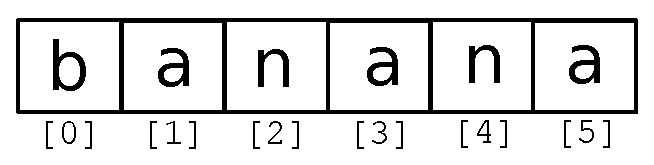
\includegraphics[height=0.50in]{figs2/string.eps}}
\afterfig

\index{index!starting at zero}
\index{zero, index starting at}

You can use any expression, including variables and operators, as an
index, but the value of the index has to be an integer.  Otherwise you
get:

\index{index}
\index{exception!TypeError}
\index{TypeError}

\beforeverb
\begin{verbatim}
>>> letter = fruit[1.5]
TypeError: string indices must be integers
\end{verbatim}
\afterverb
%

\section{Getting the length of a string using {\tt len}}

\index{len function}
\index{function!len}

{\tt len} is a built-in function that returns the number of characters
in a string:

\beforeverb
\begin{verbatim}
>>> fruit = 'banana'
>>> len(fruit)
6
\end{verbatim}
\afterverb
%
To get the last letter of a string, you might be tempted to try something
like this:

\index{exception!IndexError}
\index{IndexError}

\beforeverb
\begin{verbatim}
>>> length = len(fruit)
>>> last = fruit[length]
IndexError: string index out of range
\end{verbatim}
\afterverb
%
The reason for the {\tt IndexError} is that there is no letter in {\tt
'banana'} with the index 6.  Since we started counting at zero, the
six letters are numbered 0 to 5.  To get the last character, you have
to subtract 1 from {\tt length}:

\beforeverb
\begin{verbatim}
>>> last = fruit[length-1]
>>> print last
a
\end{verbatim}
\afterverb
%
Alternatively, you can use negative indices, which count backward from
the end of the string.  The expression {\tt fruit[-1]} yields the last
letter, {\tt fruit[-2]} yields the second to last, and so on.

\index{index!negative}
\index{negative index}


\section{Traversal through a string with a {\tt for} loop}
\label{for}

\index{traversal}
\index{loop!traversal}
\index{for loop}
\index{loop!for}
\index{statement!for}
\index{traversal}

A lot of computations involve processing a string one character at a
time.  Often they start at the beginning, select each character in
turn, do something to it, and continue until the end.  This pattern of
processing is called a {\bf traversal}.  One way to write a traversal
is with a {\tt while} loop:

\beforeverb
\begin{verbatim}
index = 0
while index < len(fruit):
    letter = fruit[index]
    print letter
    index = index + 1
\end{verbatim}
\afterverb
%
This loop traverses the string and displays each letter on a line by
itself.  The loop condition is {\tt index < len(fruit)}, so
when {\tt index} is equal to the length of the string, the
condition is false, and the body of the loop is not executed.  The
last character accessed is the one with the index {\tt len(fruit)-1},
which is the last character in the string.

\begin{ex}
Write a {\tt while} loop that starts at the last character in the string
and works its way backwards to the first character in the string, 
printing each letter on a separate line, except backwards.
\end{ex}

Another way to write a traversal is with a {\tt for} loop:

\beforeverb
\begin{verbatim}
for char in fruit:
    print char
\end{verbatim}
\afterverb
%
Each time through the loop, the next character in the string is assigned
to the variable {\tt char}.  The loop continues until no characters are
left.

\index{concatenation}
\index{abecedarian}
\index{McCloskey, Robert}

The following example shows how to use concatenation (string addition)
and a {\tt for} loop to generate an abecedarian series (that is, in
alphabetical order).  In Robert McCloskey's book \emph{Make
Way for Ducklings}, the names of the ducklings are Jack, Kack, Lack,
Mack, Nack, Ouack, Pack, and Quack.  This loop outputs these names in
order:

\beforeverb
\begin{verbatim}
prefixes = 'JKLMNOPQ'
suffix = 'ack'

for letter in prefixes:
    print letter + suffix
\end{verbatim}
\afterverb
%
The output is:

\beforeverb
\begin{verbatim}
Jack
Kack
Lack
Mack
Nack
Oack
Pack
Qack
\end{verbatim}
\afterverb
%
Of course, that's not quite right because ``Ouack'' and
``Quack'' are misspelled.


\section{String slices}
\label{slice}

\index{slice operator}
\index{operator!slice}
\index{index!slice}
\index{string!slice}
\index{slice!string}

A segment of a string is called a {\bf slice}.  Selecting a slice is
similar to selecting a character:

\beforeverb
\begin{verbatim}
>>> s = 'Monty Python'
>>> print s[0:5]
Monty
>>> print s[6:13]
Python
\end{verbatim}
\afterverb
%
The operator {\tt [n:m]} returns the part of the string from the 
``n-eth'' character to the ``m-eth'' character, including the first but
excluding the last.  This behavior is counterintuitive, but it might
help to imagine the indices pointing \emph{between} the
characters, as in the following diagram:

\beforefig
\centerline{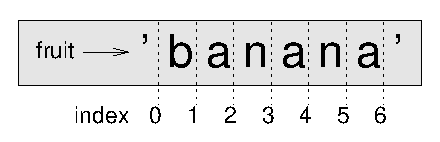
\includegraphics{figs/banana.eps}}
\afterfig

If you omit the first index (before the colon), the slice starts at
the beginning of the string.  If you omit the second index, the slice
goes to the end of the string:

\beforeverb
\begin{verbatim}
>>> fruit = 'banana'
>>> fruit[:3]
'ban'
>>> fruit[3:]
'ana'
\end{verbatim}
\afterverb
%
If the first index is greater than or equal to the second the result
is an {\bf empty string}, represented by two quotation marks:

\index{quotation mark}

\beforeverb
\begin{verbatim}
>>> fruit = 'banana'
>>> fruit[3:3]
''
\end{verbatim}
\afterverb
%
An empty string contains no characters and has length 0, but other
than that, it is the same as any other string.

\begin{ex}
Given that {\tt fruit} is a string, what does
{\tt fruit[:]} mean?

\index{copy!slice}
\index{slice!copy}


\end{ex}


\section{Strings are immutable}
\index{mutability}
\index{immutability}
\index{string!immutable}

It is tempting to use the {\tt []} operator on the left side of an
assignment, with the intention of changing a character in a string.
For example:

\index{TypeError}
\index{exception!TypeError}

\beforeverb
\begin{verbatim}
>>> greeting = 'Hello, world!'
>>> greeting[0] = 'J'
TypeError: object does not support item assignment
\end{verbatim}
\afterverb
%
The ``object'' in this case is the string and the ``item'' is
the character you tried to assign.  For now, an {\bf object} is
the same thing as a value, but we will refine that definition
later.  An {\bf item} is one of the values in a sequence.

\index{object}
\index{item assignment}
\index{assignment!item}
\index{immutability}

The reason for the error is that
strings are {\bf immutable}, which means you can't change an
existing string.  The best you can do is create a new string
that is a variation on the original:

\beforeverb
\begin{verbatim}
>>> greeting = 'Hello, world!'
>>> new_greeting = 'J' + greeting[1:]
>>> print new_greeting
Jello, world!
\end{verbatim}
\afterverb
%
This example concatenates a new first letter onto
a slice of {\tt greeting}.  It has no effect on
the original string.

\index{concatenation}


\section{Searching}
\label{find}

What does the following function do?

\index{find function}
\index{function!find}

% TBD - De-function

\beforeverb
\beforeverb
\begin{verbatim}
def find(word, letter):
    index = 0
    while index < len(word):
        if word[index] == letter:
            return index
        index = index + 1
    return -1
\end{verbatim}
\afterverb
%
In a sense, {\tt find} is the opposite of the {\tt []} operator.
Instead of taking an index and extracting the corresponding character,
it takes a character and finds the index where that character first
appears.  If the character is not found, the function returns {\tt
-1}.

This is the first example we have seen of a {\tt return} statement
inside a loop.  If {\tt word[index] == letter}, the function breaks
out of the loop and returns immediately.

If the character doesn't appear in the string, the loop
exits normally at the bottom and returns {\tt -1}.

This pattern of computation---traversing a sequence and returning
when we find what we are looking for---is a called a {\bf search}.

\index{traversal}
\index{search pattern}
\index{pattern!search}

\begin{ex}
Modify {\tt find} so that it has a
third parameter, the index in {\tt word} where it should start
looking.
\end{ex}


\section{Looping and counting}
\label{counter}

\index{counter}
\index{counting and looping}
\index{looping and counting}
\index{looping!with strings}

The following program counts the number of times the letter {\tt a}
appears in a string:

\beforeverb
\begin{verbatim}
word = 'banana'
count = 0
for letter in word:
    if letter == 'a':
        count = count + 1
print count
\end{verbatim}
\afterverb
%
This program demonstrates another pattern of computation called a {\bf
counter}.  The variable {\tt count} is initialized to 0 and then
incremented each time an {\tt a} is found.
When the loop exits, {\tt count}
contains the result---the total number of {\tt a}'s.

\begin{ex}
\index{encapsulation}

Encapsulate this code in a function named {\tt
count}, and generalize it so that it accepts the string and the
letter as arguments.
\end{ex}

\section{The {\tt in} operator}
\label{inboth}

\index{in operator}
\index{operator!in}
\index{boolean operator}
\index{operator!boolean}

The word {\tt in} is a boolean operator that takes two strings and
returns {\tt True} if the first appears as a substring in the second:

\beforeverb
\begin{verbatim}
>>> 'a' in 'banana'
True
>>> 'seed' in 'banana'
False
\end{verbatim}
\afterverb
%

\section{String comparison}

\index{string!comparison}
\index{comparison!string}

The comparison operators work on strings.  To see if two strings are equal:

\beforeverb
\begin{verbatim}
if word == 'banana':
    print  'All right, bananas.'
\end{verbatim}
\afterverb
%
Other comparison operations are useful for putting words in alphabetical
order:

\beforeverb
\begin{verbatim}
if word < 'banana':
    print 'Your word,' + word + ', comes before banana.'
elif word > 'banana':
    print 'Your word,' + word + ', comes after banana.'
else:
    print 'All right, bananas.'
\end{verbatim}
\afterverb
%
Python does not handle uppercase and lowercase letters the same way
that people do.  All the uppercase letters come before all the
lowercase letters, so:

\beforeverb
\begin{verbatim}
Your word, Pineapple, comes before banana.
\end{verbatim}
\afterverb
%
A common way to address this problem is to convert strings to a
standard format, such as all lowercase, before performing the
comparison.  Keep that in mind in case you have to defend yourself
against a man armed with a Pineapple.


\section{{\tt string} methods}

Strings are an example of Python {\bf objects}.  An object contains
both data (the actual string itself) as well as {\bf methods} which
are effectively functions which are built into the object and 
available to any {\bf instance} of the object.

Python has a function called {\tt dir} that lists the methods available
for an object.  The {\tt type} function shows the type of an object 
and the {\tt dir} function shows the available methods.
\beforeverb
\begin{verbatim}
>>> stuff = 'Hello world'
>>> type(stuff)
<type 'str'>
>>> dir(stuff)
['capitalize', 'center', 'count', 'decode', 'encode', 
'endswith', 'expandtabs', 'find', 'format', 'index', 
'isalnum', 'isalpha', 'isdigit', 'islower', 'isspace', 
'istitle', 'isupper', 'join', 'ljust', 'lower', 'lstrip', 
'partition', 'replace', 'rfind', 'rindex', 'rjust', 
'rpartition', 'rsplit', 'rstrip', 'split', 'splitlines', 
'startswith', 'strip', 'swapcase', 'title', 'translate', 
'upper', 'zfill']
>>> help(str.capitalize)
Help on method_descriptor:

capitalize(...)
    S.capitalize() -> string
    
    Return a copy of the string S with only its first character
    capitalized.
>>>
\end{verbatim}
\afterverb
%

While the {\tt dir} function lists the methods, and you 
can use {\tt help} to get some simple documentation on a method, 
a better source of documentation for string methods would be
\url{docs.python.org/library/string.html}.

Calling a {\bf method} is similar to calling a function---it 
takes arguments and
returns a value---but the syntax is different.  We call a method
by appending the method name to the variable name using the period 
as a delimiter.

For example, the
method {\tt upper} takes a string and returns a new string with
all uppercase letters:

\index{method}
\index{string!method}

Instead of the function syntax {\tt upper(word)}, it uses
the method syntax {\tt word.upper()}.

\index{dot notation}

\beforeverb
\begin{verbatim}
>>> word = 'banana'
>>> new_word = word.upper()
>>> print new_word
BANANA
\end{verbatim}
\afterverb
%
This form of dot notation specifies the name of the method, {\tt
upper}, and the name of the string to apply the method to, {\tt
word}.  The empty parentheses indicate that this method takes no
argument.

\index{parentheses!empty}

A method call is called an {\bf invocation}; in this case, we would
say that we are invoking {\tt upper} on the {\tt word}.

\index{invocation}

As it turns out, there is a string method named {\tt find} that
is remarkably similar to the function we wrote:

\beforeverb
\begin{verbatim}
>>> word = 'banana'
>>> index = word.find('a')
>>> print index
1
\end{verbatim}
\afterverb
%
In this example, we invoke {\tt find} on {\tt word} and pass
the letter we are looking for as a parameter.

Actually, the {\tt find} method is more general than our function;
it can find substrings, not just characters:

\beforeverb
\begin{verbatim}
>>> word.find('na')
2
\end{verbatim}
\afterverb
%
It can take as a second argument the index where it should start:

\index{optional argument}
\index{argument!optional}

\beforeverb
\begin{verbatim}
>>> word.find('na', 3)
4
\end{verbatim}
\afterverb
%
One common task is to remove white space (spaces, tabs, or newlines) from
the beginning and end of a string using the {\tt strip} method:

\beforeverb
\begin{verbatim}
>>> line = '  Here we go  '
>>> line.strip()
'Here we go'
\end{verbatim}
\afterverb
%
Some methods such as {\bf startswith} return boolean values.

\beforeverb
\begin{verbatim}
>>> line = 'Please have a nice day'
>>> line.startswith('Please')
True
>>> line.startswith('p')
False
\end{verbatim}
\afterverb
%
You will note that {\tt startswith} requires case to match so sometimes
we take a line and map it all to lowercase before we do any checking
using the {\tt lower} method.

\beforeverb
\begin{verbatim}
>>> line = 'Please have a nice day'
>>> line.startswith('p')
False
>>> line.lower()
'please have a nice day'
>>> line.lower().startswith('p')
True
\end{verbatim}
\afterverb
%
In the last example, the method {\tt lower} is called
and then we use {\tt startswith}
to check to see if the resulting lowercase string
starts with the letter ``p''.  As long as we are careful
with the order, we can make multiple method calls in a
single expression.

\begin{ex}
\index{count method}
\index{method!count}

There is a string method called {\tt count} that is similar
to the function in the previous exercise.  Read the documentation
of this method at
\url{docs.python.org/library/string.html}
and write an invocation that counts the number of times the 
letter a  occurs
in \verb"'banana'".
\end{ex}

\section{Parsing strings}

Often, we want to look into a string and find a substring.  For example
if we were presented a series of lines formatted as follows:

{\tt
From stephen.marquard@{\bf uct.ac.za} Sat Jan  5 09:14:16 2008
}

And we wanted to pull out only the second half of the address (i.e.
{\tt uct.ac.za}) from each line.  We can do this by using the {\tt find}
method and string slicing.   

First, we will find the position of the at-sign in the string.  Then we will
find the position of the first space \emph{after} the at-sign.  And then we
will use string slicing to extract the portion of the string which we 
are looking for.

\beforeverb
\begin{verbatim}
>>> data = 'From stephen.marquard@uct.ac.za Sat Jan  5 09:14:16 2008'
>>> atpos = data.find('@')
>>> print atpos
21
>>> sppos = data.find(' ',atpos)
>>> print sppos
31
>>> host = data[atpos+1:sppos]
>>> print host
uct.ac.za
>>> 
\end{verbatim}
\afterverb
%
We use a version of the {\tt find} method which allows us to specify
a position in the string where we want {\tt find} to start looking.
When we slice, we extract the characters 
from ``one beyond the at-sign through up to \emph{but not including} the 
space character''.  

The documentation for the {\tt find} method is available at
\url{docs.python.org/library/string.html}.

\section{Format operator}

\index{format operator}
\index{operator!format}

The {\bf format operator}, {\tt \%}
allows us to construct strings, replacing parts of the strings
with the data stored in variables.
When applied to integers, {\tt \%} is the modulus operator.  But
when the first operand is a string, {\tt \%} is the format operator.

\index{format string}

The first operand is the {\bf format string}, which contains
one or more {\bf format sequences}, which
specify how
the second operand is formatted.  The result is a string.

\index{format sequence}

For example, the format sequence \verb"'%d'" means that
the second operand should be formatted as an
integer ({\tt d} stands for ``decimal''):

\beforeverb
\begin{verbatim}
>>> camels = 42
>>> '%d' % camels
'42'
\end{verbatim}
\afterverb
%
The result is the string \verb"'42'", which is not to be confused
with the integer value {\tt 42}.

A format sequence can appear anywhere in the string,
so you can embed a value in a sentence:

\beforeverb
\begin{verbatim}
>>> camels = 42
>>> 'I have spotted %d camels.' % camels
'I have spotted 42 camels.'
\end{verbatim}
\afterverb
%
If there is more than one format sequence in the string,
the second argument has to be a tuple.  Each format sequence is
matched with an element of the tuple, in order.

The following example uses \verb"'%d'" to format an integer,
\verb"'%g'" to format
a floating-point number (don't ask why), and \verb"'%s'" to format
a string:

\beforeverb
\begin{verbatim}
>>> 'In %d years I have spotted %g %s.' % (3, 0.1, 'camels')
'In 3 years I have spotted 0.1 camels.'
\end{verbatim}
\afterverb
%
The number of elements in the tuple has to match the number
of format sequences in the string.  Also, the types of the
elements have to match the format sequences:

\index{exception!TypeError}
\index{TypeError}

\beforeverb
\begin{verbatim}
>>> '%d %d %d' % (1, 2)
TypeError: not enough arguments for format string
>>> '%d' % 'dollars'
TypeError: illegal argument type for built-in operation
\end{verbatim}
\afterverb
%
In the first example, there aren't enough elements; in the
second, the element is the wrong type.

The format operator is powerful, but it can be difficult to use.  You
can read more about it at
\url{docs.python.org/lib/typesseq-strings.html}.

% You can specify the number of digits as part of the format sequence.
% For example, the sequence \verb"'%8.2f'"
% formats a floating-point number to be 8 characters long, with
% 2 digits after the decimal point:

% \beforeverb
% \begin{verbatim}
% >>> '%8.2f' % 3.14159
% '    3.14'
% \end{verbatim}
% \afterverb
% %
% The result takes up eight spaces with two
% digits after the decimal point.  


\section{Debugging}
\index{debugging}

A skill that you should cultivate as you program is always
asking yourself, ``What could go wrong here?'' or alternatively,
``What crazy thing might our user do to crash our (seemingly) 
perfect program?''.

For example, look at the program which we used to demonstrate
the {\tt while} loop in the chapter on iteration:

\beforeverb
\begin{verbatim}
while True:
    line = raw_input('> ')
    if line[0] == '#' :
        continue
    if line == 'done':
        break
    print line

print 'Done!'
\end{verbatim}
\afterverb
%
Look what happens when the user enters an empty line of input:

\beforeverb
\begin{verbatim}
> hello there
hello there
> # don't print this
> print this!
print this!
> 
Traceback (most recent call last):
  File "copytildone.py", line 3, in <module>
    if line[0] == '#' :
\end{verbatim}
\afterverb
%
The code works fine until it is presented an empty line.  Then
there is no zeroth character so we get a traceback.  There are two
solutions to this to make line three ``safe'' even if the line is 
empty.

One possibility is to simply use the {\tt startswith} method
which returns {\tt False} if the string is empty.

\beforeverb
\begin{verbatim}
    if line.startswith('#') :
\end{verbatim}
\afterverb
%
\index{guardian pattern}
\index{pattern!guardian}
Another way to safely write the {\tt if} statement using the {\bf guardian}
pattern and make sure the second logical expression is evaluated 
only where there is at least one character in the string.:

\beforeverb
\begin{verbatim}
    if len(line) > 0 and line[0] == '#' :
\end{verbatim}
\afterverb
%

\index{traversal}

Another common source of problems is when you hand-construct 
index values to move through a sequence.
It can be quite tricky to get the beginning and 
end of the traversal right. 

Here is a function that is supposed to compare two
words and return {\tt True} if one of the words is the reverse
of the other, but it contains two errors:

\beforeverb
\begin{verbatim}
def is_reverse(word1, word2):
    if len(word1) != len(word2):
        return False
    
    i = 0
    j = len(word2)

    while j > 0:
        if word1[i] != word2[j]:
            return False
        i = i+1
        j = j-1

    return True
\end{verbatim}
\afterverb
%
The first {\tt if} statement checks whether the words are the
same length.  If not, we can return {\tt False} immediately
and then, for the rest of the function, we can assume that the words
are the same length.  This is another example of the guardian pattern.

\index{guardian pattern}
\index{pattern!guardian}
\index{index}

{\tt i} and {\tt j} are indices: {\tt i} traverses {\tt word1}
forward while {\tt j} traverses {\tt word2} backward.  If we find
two letters that don't match, we can return {\tt False} immediately.
If we get through the whole loop and all the letters match, we
return {\tt True}.

If we test this function with the words ``pots'' and ``stop'', we
expect the return value {\tt True}, but we get an IndexError:

\index{IndexError}
\index{exception!IndexError}

\beforeverb
\begin{verbatim}
>>> is_reverse('pots', 'stop')
...
  File "reverse.py", line 15, in is_reverse
    if word1[i] != word2[j]:
IndexError: string index out of range
\end{verbatim}
\afterverb
%
For debugging this kind of error, my first move is to
print the values of the indices immediately before the line
where the error appears.

\beforeverb
\begin{verbatim}
    while j > 0:
        print i, j        # print here
        
        if word1[i] != word2[j]:
            return False
        i = i+1
        j = j-1
\end{verbatim}
\afterverb
%
Now when I run the program again, I get more information:

\beforeverb
\begin{verbatim}
>>> is_reverse('pots', 'stop')
0 4
...
IndexError: string index out of range
\end{verbatim}
\afterverb
%
The first time through the loop, the value of {\tt j} is 4,
which is out of range for the string \verb"'pots'".
The index of the last character is 3, so the
initial value for {\tt j} should be {\tt len(word2)-1}.

\index{semantic error}
\index{error!semantic}

If I fix that error and run the program again, I get:

\beforeverb
\begin{verbatim}
>>> is_reverse('pots', 'stop')
0 3
1 2
2 1
True
\end{verbatim}
\afterverb
%
This time we get the right answer, but it looks like the loop only ran
three times, which is suspicious.  To get a better idea of what is
happening, it is useful to draw a state diagram.  During the first
iteration, the frame for \verb"is_reverse" looks like this:

\index{state diagram}
\index{diagram!state}

\beforefig
\centerline{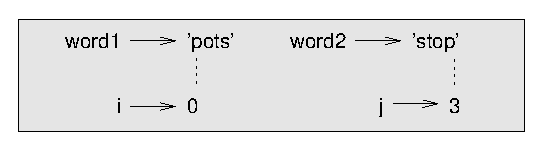
\includegraphics{figs/state4.eps}}
\afterfig

I took a little license by arranging the variables in the frame
and adding dotted lines to show that the values of {\tt i} and
{\tt j} indicate characters in {\tt word1} and {\tt word2}.

\begin{ex}
\label{is_reverse}
Starting with this diagram, execute the program on paper, changing the
values of {\tt i} and {\tt j} during each iteration.  Find and fix the
second error in this function.
\end{ex}



\section{Glossary}

\begin{description}

\item[counter:] A variable used to count something, usually initialized
to zero and then incremented.
\index{counter}

\item[empty string:] A string with no characters and length 0, represented
by two quotation marks.
\index{empty string}

\item[format operator:] An operator, {\tt \%}, that takes a format
string and a tuple and generates a string that includes
the elements of the tuple formatted as specified by the format string.
\index{format operator}
\index{operator!format}

\item[format sequence:] A sequence of characters in a format string,
like {\tt \%d}, that specifies how a value should be formatted.
\index{format sequence}

\item[format string:] A string, used with the format operator, that
contains format sequences.
\index{format string}

\item[flag:] A boolean variable used to indicate whether a condition
is true.
\index{flag}

\item[invocation:] A statement that calls a method.
\index{invocation}

\item[immutable:] The property of a sequence whose items cannot
be assigned.
\index{immutability}

\item[index:] An integer value used to select an item in
a sequence, such as a character in a string.
\index{index}

\item[item:] One of the values in a sequence.
\index{item}

\item[method:] A function that is associated with an object and called
using dot notation.
\index{method}

\item[object:] Something a variable can refer to.  For now,
you can use ``object'' and ``value'' interchangeably.
\index{object}

\item[search:] A pattern of traversal that stops
when it finds what it is looking for.
\index{search pattern}
\index{pattern!search}

\item[sequence:] An ordered set; that is, a set of
values where each value is identified by an integer index.
\index{sequence}

\item[slice:] A part of a string specified by a range of indices.
\index{slice}

\item[traverse:] To iterate through the items in a sequence,
performing a similar operation on each.
\index{traversal}

\end{description}


\section{Exercises}

\begin{ex}
Write some code to parse lines of the form:

{\tt
X-DSPAM-Confidence: {\bf 0.8475}
}

Use {\tt find} and string slicing to extract the portion
of the string after the colon character and then use the 
{\tt float} function to convert the extracted string 
into a floating point number.

\end{ex}


\begin{ex}
\index{string method}
\index{method!string}

Read the documentation of the string methods at
\url{docs.python.org/lib/string-methods.html}.  You
might want to experiment with some of them to make sure
you understand how they work.  {\tt strip} and
{\tt replace} are particularly useful.

The documentation uses a syntax that might be confusing.
For example, in \verb"find(sub[, start[, end]])", the brackets
indicate optional arguments.  So {\tt sub} is required, but
{\tt start} is optional, and if you include {\tt start},
then {\tt end} is optional.
\end{ex}

\begin{ex}
The following functions are all \emph{intended} to check whether a
string contains any lowercase letters, but at least some of them are
wrong.  For each function, describe what the function actually does
(assuming that the parameter is a string).

\beforeverb
\begin{verbatim}
def any_lowercase1(s):
    for c in s:
        if c.islower():
            return True
        else:
            return False

def any_lowercase2(s):
    for c in s:
        if 'c'.islower():
            return 'True'
        else:
            return 'False'

def any_lowercase3(s):
    for c in s:
        flag = c.islower()
    return flag

def any_lowercase4(s):
    flag = False
    for c in s:
        flag = flag or c.islower()
    return flag

def any_lowercase5(s):
    for c in s:
        if not c.islower():
            return False
    return True
\end{verbatim}
\afterverb

\end{ex}


\begin{ex}
\index{letter rotation}
\index{rotation, letter}

\label{exrotate}
ROT13 is a weak form of encryption that involves ``rotating'' each
letter in a word by 13 places\footnote{See
  \url{wikipedia.org/wiki/ROT13}}.  To rotate a letter means
to shift it through the alphabet, wrapping around to the beginning if
necessary, so 'A' shifted by 3 is 'D' and 'Z' shifted by 1 is 'A'.

Write a function called \verb"rotate_word"
that takes a string and an integer as parameters and returns
a new string that contains the letters from the original string
``rotated'' by the given amount.  

For example, ``cheer'' rotated by 7 is ``jolly'' and ``melon'' rotated
by -10 is ``cubed''.  

%For example ``sleep''
%rotated by 9 is ``bunny'' and ``latex'' rotated by 7 is ``shale''.

You might want to use the built-in functions {\tt ord}, which converts
a character to a numeric code, and {\tt chr}, which converts numeric
codes to characters.

Potentially offensive jokes on the Internet are sometimes encoded
in ROT13.  If you are not easily offended, find and decode some
of them.
\end{ex}

\chapter{Files}

\index{file}
\index{type!file}


\section{Persistence}

\index{persistence}
\index{secondary memory}

So far, we have learned how to write programs and communicate 
our intentions to the {\bf Central Processing Unit} using conditional
execution, functions, and iterations.  We have learned how to 
create and use data structures in the {\bf Main Memory}.  The CPU 
and memory are where our software works and runs.  It is where 
all of the ``thinking'' happens.  

But if you recall from our hardware architecture discussions,
once the power is turned off, anything stored in either
the CPU or main memory is erased.  So up to now, our
programs have just been transient fun exercises to learn Python.

\beforefig
\centerline{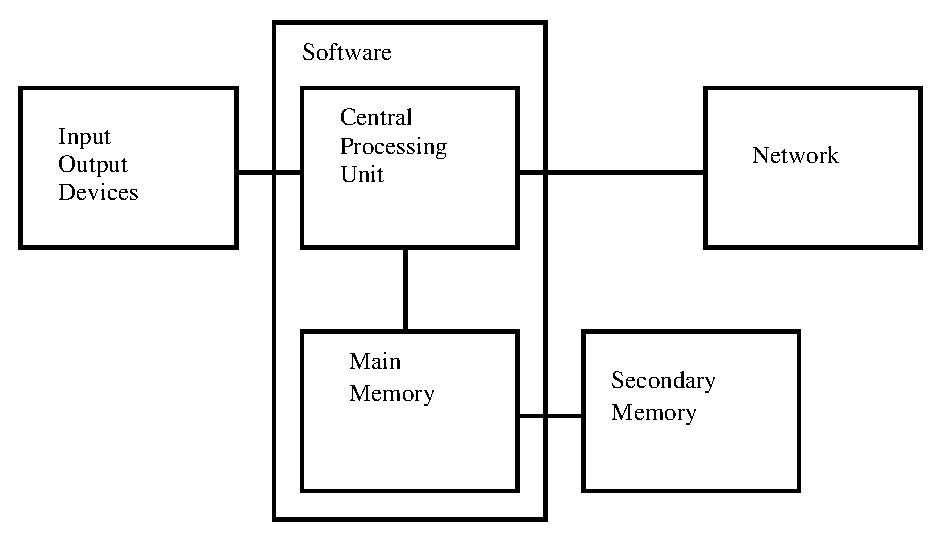
\includegraphics[height=2.50in]{figs2/arch3.eps}}
\afterfig

In this chapter, we start to work with {\bf Secondary Memory} 
(or files).
Secondary memory is not erased even when the power is turned off.  
Or in the case of a USB flash drive, the
data can we write from our programs can be removed from the 
system and transported to another system.

We will primarily focus on reading and writing text files such as 
those we create in a text editor.  Later we will see how to work
with database files which are binary files, specifically designed to be read
and written through database software.

\section{Opening files}
\index{file!open}
\index{open function}
\index{function!open}

When we want to read or write a file (say on your hard drive), we first
must {\bf open} the file.  Opening the file communicates with your operating
system which knows where the data for each file is stored.  When you open
a file, you are asking the operating system to find the file by name
and make sure the file exists.  In this example, we open the file 
{\tt mbox.txt} which should be stored in the same folder that you
are in when you 
start Python.
You can download this file from 
\url{www.py4inf.com/code/mbox.txt}

\beforeverb
\begin{verbatim}
>>> fhand = open('mbox.txt')
>>> print fhand
<open file 'mbox.txt', mode 'r' at 0x1005088b0>
\end{verbatim}
\afterverb
%
\index{file handle}
If the {\tt open} is successful, the operating system returns us a 
{\bf file handle}.  The file handle is not the actual data contained
in the file, but instead it is a ``handle'' that we can use to 
read the data.   You are given a handle if the requested file
exists and you have the proper permissions to read the file.

\beforefig
\centerline{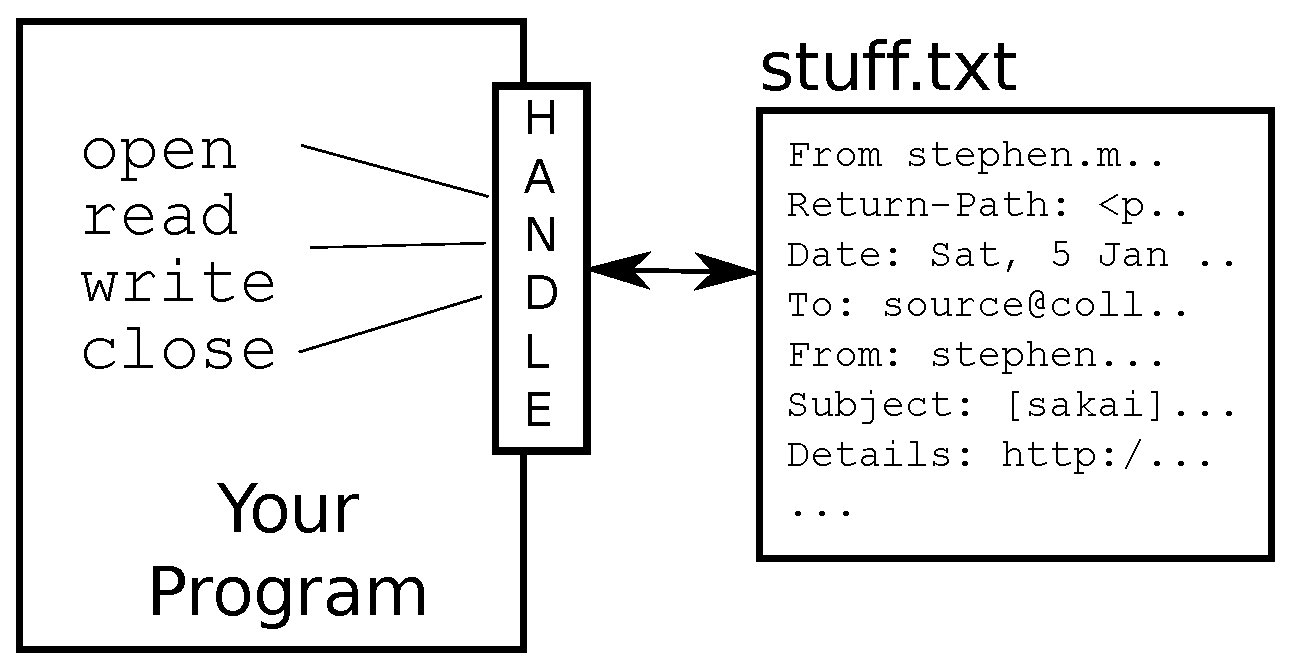
\includegraphics[height=1.75in]{figs2/handle.eps}}
\afterfig

If the file does not exist, {\tt open} will fail with a traceback and you 
will not get a handle to access the contents of the file:

\beforeverb
\begin{verbatim}
>>> fhand = open('stuff.txt')
Traceback (most recent call last):
  File "<stdin>", line 1, in <module>
IOError: [Errno 2] No such file or directory: 'stuff.txt'
\end{verbatim}
\afterverb
%
Later we will use {\tt try} and {\tt except} to deal more gracefully
with the situation where we attempt to open a file that does 
not exist.

\section{Text files and lines}

A text file can be thought of as a sequence of lines, much like a Python
string can be thought of as a sequence of characters.  For example, this
is a sample of a text file which records mail activity from various
individuals in an open source project development team:

{\tt
From stephen.marquard@uct.ac.za Sat Jan  5 09:14:16 2008\\
Return-Path: <postmaster@collab.sakaiproject.org>\\
Date: Sat, 5 Jan 2008 09:12:18 -0500\\
To: source@collab.sakaiproject.org\\
From: stephen.marquard@uct.ac.za\\
Subject: [sakai] svn commit: r39772 - content/branches/\\
Details: http://source.sakaiproject.org/viewsvn/?view=rev\&rev=39772\\
...
}

The entire file of mail interactions is available from 
\url{www.py4inf.com/code/mbox.txt} 
and a shortened version of the file is available from
\url{www.py4inf.com/code/mbox-short.txt}.
These files are in a standard format for a file containing 
multiple mail messages. The lines which start with 
``From '' separate the messages and the lines which start 
with ``From:'' are part of the messages. 
For more information, see 
\url{en.wikipedia.org/wiki/Mbox}. 

To break the file into lines, there is a special character that 
represents the ``end of the line'' called the {\bf newline} character.

\index{newline}
In Python, we represent the {\bf newline} character as a backslash-n in 
string constants.  Even though this looks like two characters, it
is actually a single character.  When we look at the variable by entering
``stuff'' in the interpreter, it shows us the \verb"\n" in the string, 
but when we use {\tt print} to show the string, we see the string broken
into two lines by the newline character.

\beforeverb
\begin{verbatim}
>>> stuff = 'Hello\nWorld!'
>>> stuff
'Hello\nWorld!'
>>> print stuff
Hello
World!
>>> stuff = 'X\nY'
>>> print stuff
X
Y
>>> len(stuff)
3
\end{verbatim}
\afterverb
%

You can also see that the length of the string \verb"'X\nY'" is \emph{three}
characters because the newline character is a single character.

So when we look at the lines in a file, we need to \emph{imagine}
that there is a special invisible character at the end of each line
that marks the end of the line called the newline.  

{\tt
From stephen.marquard@uct.ac.za Sat Jan  5 09:14:16 2008\verb"\n"\\
Return-Path: <postmaster@collab.sakaiproject.org>\verb"\n"\\
Date: Sat, 5 Jan 2008 09:12:18 -0500\verb"\n"\\
To: source@collab.sakaiproject.org\verb"\n"\\
From: stephen.marquard@uct.ac.za\verb"\n"\\
Subject: [sakai] svn commit: r39772 - content/branches/\verb"\n"\\
Details: http://source.sakaiproject.org/viewsvn/?view=rev\&rev=39772\verb"\n"\\
...
}

So the newline character separates the characters 
in the file into lines.

\section{Reading files}

\index{file!reading}
\index{counter}
While the {\bf file handle} does not contain the data for the file,
it is quite easy to construct a {\tt for} loop to read through 
and count each of the lines in a file:

\beforeverb
\begin{verbatim}
fhand = open('mbox.txt')
count = 0
for line in fhand:
    count = count + 1
print 'Line Count:', count

python open.py 
Line Count: 132045
\end{verbatim}
\afterverb
%
We can use the file handle as the sequence in our {\tt for} loop.  
Our {\tt for} loop simply counts the number of lines in the 
file and prints them out.  The rough translation of the {\tt for}
loop into English is, ``for each line in the file represented by the file
handle, add one to the {\tt count} variable.''

The reason that the {\tt open} function does not read the entire file
is that the file might be quite large with many gigabytes of data.
The {\tt open} statement takes the same amount of time regardless of the
size of the file.  The {\tt for} loop actually causes the data to be 
read from the file.

When the file is read using a {\tt for} loop in this manner, Python
takes care of splitting the data in the file into separate lines using
the newline character.  Python reads each line through 
the newline and includes
the newline as the last character in the {\tt line} variable for each 
iteration of the {\tt for} loop.

Because the for loop reads the data one line at a time, it can efficiently
read and count the lines in very large files without running 
out of main memory to store the data.  The above program can 
count the lines in any size file using very little memory since 
each line is read, counted, and then discarded.

If you know the file is relatively small compared to the size of 
your main memory, you can read the whole file into one string
using the {\tt read} method on the file handle.

\beforeverb
\begin{verbatim}
>>> fhand = open('mbox-short.txt')
>>> inp = fhand.read()
>>> print len(inp)
94626
>>> print inp[:20]
From stephen.marquar
\end{verbatim}
\afterverb
%
In this example, the entire contents (all 94,626 characters) 
of the file {\tt mbox-short.txt} are read directly into the 
variable {\tt inp}.  We use string slicing to print out the first
20 characters of the string data stored in {\tt inp}.

When the file is read in this manner, all the characters including 
all of the lines and newline characters are one big string 
in the variable {\bf inp}.  
Remember that this form of the {\tt open} function should only be used
if the file data will fit comfortably in the main memory 
of your computer.

If the file is too large to fit in main memory, you should write
your program to read the file in chunks using a {\tt for} or {\tt while}
loop.

\section{Searching through a file}

When you are searching through data in a file, it
is a very common pattern to read through a file, ignoring most
of the lines and only processing lines which meet a particular criteria.
We can combine the pattern for reading a file with string {\bf methods}
to build simple search mechanisms.

\index{filter pattern}
\index{pattern!filter}
For example, if we wanted to read a file and only print out lines
which started with the prefix ``From:'', we could use the 
string method {\bf startswith} to select only those lines with
the desired prefix:

\beforeverb
\begin{verbatim}
fhand = open('mbox-short.txt')
for line in fhand:
    if line.startswith('From:') :
        print line
\end{verbatim}
\afterverb
%
When this program runs, we get the following output:

\beforeverb
\begin{verbatim}
From: stephen.marquard@uct.ac.za

From: louis@media.berkeley.edu

From: zqian@umich.edu

From: rjlowe@iupui.edu
...
\end{verbatim}
\afterverb
%
The output looks great since the only lines we are seeing are those 
which start with ``From:'', but why are we seeing the extra blank
lines?  This is due to that invisible {\bf newline} character.
Each of the lines ends with a newline, so the {\tt print} 
statement prints the string in the variable {\bf line} which includes
a newline and then {\tt print} adds \emph{another} newline, resulting
in the double spacing effect we see.

We could use line slicing to print all but the last character, but 
a simpler approach is to use the {\bf rstrip} method which strips
whitespace from the right side of a string as follows:

\beforeverb
\begin{verbatim}
fhand = open('mbox-short.txt')
for line in fhand:
    line = line.rstrip()
    if line.startswith('From:') :
        print line
\end{verbatim}
\afterverb
%
When this program runs, we get the following output:

\beforeverb
\begin{verbatim}
From: stephen.marquard@uct.ac.za
From: louis@media.berkeley.edu
From: zqian@umich.edu
From: rjlowe@iupui.edu
From: zqian@umich.edu
From: rjlowe@iupui.edu
From: cwen@iupui.edu
...
\end{verbatim}
\afterverb
%
As your file processing programs get more complicated, you may want 
to structure your search loops using {\tt continue}.  The basic idea 
of the search loop is that you are looking for ``interesting'' lines
and effectively skipping ``uninteresting'' lines.  And then when we
find an interesting line, we do something with that line.

We can structure the loop to follow the
pattern of skipping uninteresting lines as follows:

\beforeverb
\begin{verbatim}
fhand = open('mbox-short.txt')
for line in fhand:
    line = line.rstrip()
    # Skip 'uninteresting lines'
    if not line.startswith('From:') :
        continue
    # Process our 'interesting' line
    print line
\end{verbatim}
\afterverb
%
The output of the program is the same.  In English, the 
uninteresting lines are those which do not start 
with ``From:'', which we skip using {\tt continue}.
For the ``interesting'' lines (i.e. those that start with ``From:'')
we perform the processing on those lines.

We can use the {\tt find} string method to simulate a text editor
search which finds lines where the search string is anywhere in the line.  
Since {\tt find} looks for an occurrence of a string within another
string and either returns the position of the string or -1 if the string
was not found, we can write the following loop to show lines which
contain the string ``@uct.ac.za'' (i.e. they come from the University 
of Capetown in South Africa):

\beforeverb
\begin{verbatim}
fhand = open('mbox-short.txt')
for line in fhand:
    line = line.rstrip()
    if line.find('@uct.ac.za') == -1 : 
        continue
    print line
\end{verbatim}
\afterverb
%
Which produces the following output:

\beforeverb
\begin{verbatim}
From stephen.marquard@uct.ac.za Sat Jan  5 09:14:16 2008
X-Authentication-Warning: set sender to stephen.marquard@uct.ac.za using -f
From: stephen.marquard@uct.ac.za
Author: stephen.marquard@uct.ac.za
From david.horwitz@uct.ac.za Fri Jan  4 07:02:32 2008
X-Authentication-Warning: set sender to david.horwitz@uct.ac.za using -f
From: david.horwitz@uct.ac.za
Author: david.horwitz@uct.ac.za
...
\end{verbatim}
\afterverb
%

\section{Letting the user choose the file name}

We really do not want to have to edit our Python code
every time we want to process a different file.  It would 
be more usable to ask the user to enter the file name string 
each time the program runs so they can use our 
program on different files without changing the Python code.

This is quite simple to do by reading the file name from
the user using \verb"raw_input" as follows:

\beforeverb
\begin{verbatim}
fname = raw_input('Enter the file name: ')
fhand = open(fname)
count = 0
for line in fhand:
    if line.startswith('Subject:') :
        count = count + 1
print 'There were', count, 'subject lines in', fname
\end{verbatim}
\afterverb
%
We read the file name from the user and place it in a variable
named {\tt fname} and open that file.  Now we can run the program 
repeatedly on different files.

\beforeverb
\begin{verbatim}
python search6.py 
Enter the file name: mbox.txt
There were 1797 subject lines in mbox.txt

python search6.py 
Enter the file name: mbox-short.txt
There were 27 subject lines in mbox-short.txt
\end{verbatim}
\afterverb
%
Before peeking at the next section, take a look at the above program
and ask yourself, ``What could go possibly wrong here?'' or ``What might our
friendly user do that would cause our nice little program to 
ungracefully exit with a traceback, making us look not-so-cool 
in the eyes of our users?''.

\section{Using {\tt try, except,} and {\tt open}}

I told you not to peek.  This is your last chance.

What if our user types something that is not a file name?
\beforeverb
\begin{verbatim}
python search6.py 
Enter the file name: missing.txt
Traceback (most recent call last):
  File "search6.py", line 2, in <module>
    fhand = open(fname)
IOError: [Errno 2] No such file or directory: 'missing.txt'

python search6.py 
Enter the file name: na na boo boo
Traceback (most recent call last):
  File "search6.py", line 2, in <module>
    fhand = open(fname)
IOError: [Errno 2] No such file or directory: 'na na boo boo'
\end{verbatim}
\afterverb
%
Do not laugh, users will eventually do every possible thing they can do 
to break your programs --- either on purpose or with malicious intent.
As a matter of fact, an important part of any software development
team is a person or group called {\bf Quality Assurance} (or QA for short)
whose very job it is to do the craziest things possible in an attempt
to break the software that the programmer has created.

\index{Quality Assurance}
\index{QA}
The QA team is responsible for finding the flaws in programs before 
we have delivered the program to the end-users who may be purchasing the
software or paying our salary to write the software.  So the QA team
is the programmer's best friend.

\index{try statement}
\index{statement!try}
\index{open function}
\index{function!open}
\index{exception!IOError}
\index{IOError}
So now that we see the flaw in the program, we can elegantly fix it using
the {\tt try}/{\tt except} structure.  We need to assume that the {\tt open}
call might fail and add recovery code when the {\tt open} fails
as follows:

\beforeverb
\begin{verbatim}
fname = raw_input('Enter the file name: ')
try:
    fhand = open(fname)
except:
    print 'File cannot be opened:', fname
    exit()

count = 0
for line in fhand:
    if line.startswith('Subject:') : 
        count = count + 1
print 'There were', count, 'subject lines in', fname
\end{verbatim}
\afterverb
%
The {\tt exit} function terminates the program.  It is a function
that we call that never returns.  Now when our user (or 
QA team) types in silliness or bad file names, 
we ``catch'' them and recover gracefully:
\beforeverb
\begin{verbatim}
python search7.py
Enter the file name: mbox.txt
There were 1797 subject lines in mbox.txt

python search7.py
Enter the file name: na na boo boo
File cannot be opened: na na boo boo
\end{verbatim}
\afterverb
%
\index{Pythonic}
Protecting the {\tt open} call is a good example 
of the proper use of {\tt try}
and {\tt except} in a Python program.  We use the term
``Pythonic'' when we are doing something the ``Python
way''.  We might say that the above example is 
the Pythonic way to open a file.

Once you become more skilled in Python, you can engage
in reparte' with other Python programmers to decide
which of two equivalent solutions to a problem is 
``more Pythonic''.  The goal to be ``more Pythonic'' 
captures the notion that programming is part engineering
and part art.  We are not always interested
in just making something work, we also want
our solution to be elegant and to be appreciated as 
elegant by our peers.


\section{Writing files}

\index{file!writing}

To write a file, you have to open it with mode
\verb"'w'" as a second parameter:

\beforeverb
\begin{verbatim}
>>> fout = open('output.txt', 'w')
>>> print fout
<open file 'output.txt', mode 'w' at 0xb7eb2410>
\end{verbatim}
\afterverb
%
If the file already exists, opening it in write mode clears out
the old data and starts fresh, so be careful!
If the file doesn't exist, a new one is created.

The {\tt write} method of the file handle object 
puts data into the file.

\beforeverb
\begin{verbatim}
>>> line1 = 'This here's the wattle,\n'
>>> fout.write(line1)
\end{verbatim}
\afterverb
%
\index{newline}
Again, the file object keeps track of where it is, so if
you call {\tt write} again, it adds the new data to the end.

We must make sure to manage the ends of lines as we write
to the file by explicitly inserting the newline character
when we want to end a line.  The {\tt print} statement 
automatically appends a newline, but the {\tt write} 
method does not add the newline automatically.

\beforeverb
\begin{verbatim}
>>> line2 = 'the emblem of our land.\n'
>>> fout.write(line2)
\end{verbatim}
\afterverb
%
When you are done writing, you have to close the file
to make sure that the last bit of data is physically written
to the disk so it will not be lost if the power goes off.

\beforeverb
\begin{verbatim}
>>> fout.close()
\end{verbatim}
\afterverb
%
We could close the files which we open for read as well, 
but we can be a little sloppy if we are only opening a few
files since Python makes sure that all open files are 
closed when the program ends.  When we are writing files, 
we want to explicitly close the files so as to leave nothing
to chance.

\index{close method}
\index{method!close}


\section{Debugging}

\index{debugging}
\index{whitespace}

When you are reading and writing files, you might run into problems
with whitespace.  These errors can be hard to debug because spaces,
tabs and newlines are normally invisible:

\beforeverb
\begin{verbatim}
>>> s = '1 2\t 3\n 4'
>>> print s
1 2	 3
 4
\end{verbatim}
\afterverb

\index{repr function}
\index{function!repr}
\index{string representation}

The built-in function {\tt repr} can help.  It takes any object as an
argument and returns a string representation of the object.  For
strings, it represents whitespace
characters with backslash sequences:

\beforeverb
\begin{verbatim}
>>> print repr(s)
'1 2\t 3\n 4'
\end{verbatim}
\afterverb

This can be helpful for debugging.

One other problem you might run into is that different systems
use different characters to indicate the end of a line.  Some
systems use a newline, represented \verb"\n".  Others use
a return character, represented \verb"\r".  Some use both.
If you move files between different systems, these inconsistencies
might cause problems.

\index{end of line character}

For most systems, there are applications to convert from one
format to another.  You can find them (and read more about this
issue) at \url{wikipedia.org/wiki/Newline}.  Or, of course, you
could write one yourself.

% TBD - Doesn't Python take care of this for us????

\section{Glossary}

\begin{description}

\item[catch:] To prevent an exception from terminating
a program using the {\tt try}
and {\tt except} statements.
\index{catch}

\item[newline:] A special character used in files and strings to indicate
the end of a line.
\index{newline}

\item[Pythonic:] A technique that works elegantly in Python.
``Using try and except is the \emph{Pythonic} way to recover from 
missing files.''.
\index{Pythonic}

\item[Quality Assurance:] A person or team focused on insuring the 
overall quality of a software product.  QA is often involved 
in testing a product and identifying problems before the product 
is released.
\index{Quality Assurance}
\index{QA}

\item[text file:] A sequence of characters stored in permanent
storage like a hard drive.
\index{text file}

\end{description}


\section{Exercises}

\begin{ex}
Write a program to read through a file and print the contents 
of the file (line by line) all in upper case.  Executing the program 
will look as follows:

\beforeverb
\begin{verbatim}
python shout.py
Enter a file name: mbox-short.txt
FROM STEPHEN.MARQUARD@UCT.AC.ZA SAT JAN  5 09:14:16 2008
RETURN-PATH: <POSTMASTER@COLLAB.SAKAIPROJECT.ORG>
RECEIVED: FROM MURDER (MAIL.UMICH.EDU [141.211.14.90])
	 BY FRANKENSTEIN.MAIL.UMICH.EDU (CYRUS V2.3.8) WITH LMTPA;
	 SAT, 05 JAN 2008 09:14:16 -0500
\end{verbatim}
\afterverb
%
You can download the file from
\url{www.py4inf.com/code/mbox-short.txt}
\end{ex}

\begin{ex}
Write a program to loop through a mailbox-format file 
and look for lines of the form:

{\tt
X-DSPAM-Confidence: {\bf 0.8475}
}

When you encounter a line that starts with 
``X-DSPAM-Confidence:'' pull apart the line to extract the
floating point number on the line.  Count these 
lines and the compute the total of the spam confidence 
values from these lines.
When you reach the end of the file, print out the average
spam confidence.

\beforeverb
\begin{verbatim}
Enter the file name: mbox.txt
Average spam confidence: 0.894128046745

Enter the file name: mbox-short.txt
Average spam confidence: 0.750718518519
\end{verbatim}
\afterverb
\end{ex}

\begin{ex}
Sometimes when programmers get bored or want to have a bit of fun,
they add a harmless {\bf Easter Egg} to their program 
(\url{en.wikipedia.org/wiki/Easter_egg_(media)}). Modify the program
that prompts the user for the file name so that it prints a funny
message when the user types in the exact file name 'na na boo boo'. 
The program should behave normally for all other files which exist
and don't exist.  Here is a sample execution of the program:

\beforeverb
\begin{verbatim}
python egg.py 
Enter the file name: mbox.txt
There were 1797 subject lines in mbox.txt

python egg.py 
Enter the file name: missing.tyxt
File cannot be opened: missing.tyxt

python egg.py 
Enter the file name: na na boo boo
NA NA BOO BOO TO YOU - You have been punk'd!
\end{verbatim}
\afterverb
%
We are not encouraging you to put Easter Eggs in your programs -
this is just an exercise.

\end{ex}

\chapter{Lists}

\index{list}
\index{type!list}


\section{A list is a sequence}

Like a string, a {\bf list} is a sequence of values.  In a string, the
values are characters; in a list, they can be any type.  The values in
list are called {\bf elements} or sometimes {\bf items}.

\index{element}
\index{sequence}
\index{item}

There are several ways to create a new list; the simplest is to
enclose the elements in square brackets (\verb"[" and \verb"]"):

\beforeverb
\begin{verbatim}
[10, 20, 30, 40]
['crunchy frog', 'ram bladder', 'lark vomit']
\end{verbatim}
\afterverb
%
The first example is a list of four integers.  The second is a list of
three strings.  The elements of a list don't have to be the same type.
The following list contains a string, a float, an integer, and
(lo!) another list:

\beforeverb
\begin{verbatim}
['spam', 2.0, 5, [10, 20]]
\end{verbatim}
\afterverb
%
A list within another list is {\bf nested}.

\index{nested list}
\index{list!nested}

A list that contains no elements is
called an empty list; you can create one with empty
brackets, \verb"[]".

\index{empty list}
\index{list!empty}

As you might expect, you can assign list values to variables:

\beforeverb
\begin{verbatim}
>>> cheeses = ['Cheddar', 'Edam', 'Gouda']
>>> numbers = [17, 123]
>>> empty = []
>>> print cheeses, numbers, empty
['Cheddar', 'Edam', 'Gouda'] [17, 123] []
\end{verbatim}
\afterverb
%

\index{assignment}

% From Jeff: write sum for a nested list?


\section{Lists are mutable}

\index{list!element}
\index{access}
\index{index}
\index{bracket operator}
\index{operator!bracket}

The syntax for accessing the elements of a list is the same as for
accessing the characters of a string---the bracket operator.  The
expression inside the brackets specifies the index.  Remember that the
indices start at 0:

\beforeverb
\begin{verbatim}
>>> print cheeses[0]
Cheddar
\end{verbatim}
\afterverb
%
Unlike strings, lists are mutable.  When the bracket operator appears
on the left side of an assignment, it identifies the element of the
list that will be assigned.

\index{mutability}

\beforeverb
\begin{verbatim}
>>> numbers = [17, 123]
>>> numbers[1] = 5
>>> print numbers
[17, 5]
\end{verbatim}
\afterverb
%
The one-eth element of {\tt numbers}, which
used to be 123, is now 5.

\index{index!starting at zero}
\index{zero, index starting at}

You can think of a list as a relationship between indices and
elements.  This relationship is called a {\bf mapping}; each index
``maps to'' one of the elements.  Here is a state diagram showing {\tt
cheeses}, {\tt numbers} and {\tt empty}:

\index{state diagram}
\index{diagram!state}
\index{mapping}

\beforefig
\centerline{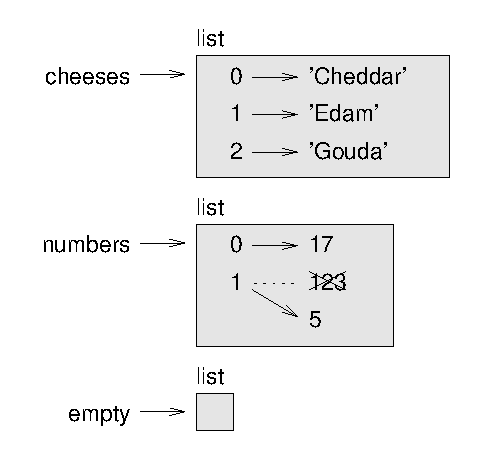
\includegraphics{figs/list_state.eps}}
\afterfig

Lists are represented by boxes with the word ``list'' outside
and the elements of the list inside.  {\tt cheeses} refers to
a list with three elements indexed 0, 1 and 2.
{\tt numbers} contains two elements; the diagram shows that the
value of the second element has been reassigned from 123 to 5.
{\tt empty} refers to a list with no elements.

\index{item assignment}
\index{assignment!item}

List indices work the same way as string indices:

\begin{itemize}

\item Any integer expression can be used as an index.

\item If you try to read or write an element that does not exist, you
get an {\tt IndexError}.

\index{exception!IndexError}
\index{IndexError}

\item If an index has a negative value, it counts backward from the
end of the list.

\end{itemize}

\index{list!index}


\index{list!membership}
\index{membership!list}
\index{in operator}
\index{operator!in}

The {\tt in} operator also works on lists.

\beforeverb
\begin{verbatim}
>>> cheeses = ['Cheddar', 'Edam', 'Gouda']
>>> 'Edam' in cheeses
True
>>> 'Brie' in cheeses
False
\end{verbatim}
\afterverb


\section{Traversing a list}
\index{list!traversal}
\index{traversal!list}
\index{for loop}
\index{loop!for}
\index{statement!for}

The most common way to traverse the elements of a list is
with a {\tt for} loop.  The syntax is the same as for strings:

\beforeverb
\begin{verbatim}
for cheese in cheeses:
    print cheese
\end{verbatim}
\afterverb
%
This works well if you only need to read the elements of the
list.  But if you want to write or update the elements, you
need the indices.  A common way to do that is to combine
the functions {\tt range} and {\tt len}:

\index{looping!with indices}
\index{index!looping with}

\beforeverb
\begin{verbatim}
for i in range(len(numbers)):
    numbers[i] = numbers[i] * 2
\end{verbatim}
\afterverb
%
This loop traverses the list and updates each element.  {\tt len}
returns the number of elements in the list.  {\tt range} returns
a list of indices from 0 to $n-1$, where $n$ is the length of
the list.  Each time through the loop {\tt i} gets the index
of the next element.  The assignment statement in the body uses
{\tt i} to read the old value of the element and to assign the
new value.

\index{item update}
\index{update!item}

A {\tt for} loop over an empty list never executes the body:

\beforeverb
\begin{verbatim}
for x in empty:
    print 'This never happens.'
\end{verbatim}
\afterverb
%
Although a list can contain another list, the nested
list still counts as a single element.  The length of this list is
four:

\index{nested list}
\index{list!nested}

\beforeverb
\begin{verbatim}
['spam', 1, ['Brie', 'Roquefort', 'Pol le Veq'], [1, 2, 3]]
\end{verbatim}
\afterverb



\section{List operations}
\index{list!operation}

The {\tt +} operator concatenates lists:

\index{concatenation!list}
\index{list!concatenation}

\beforeverb
\begin{verbatim}
>>> a = [1, 2, 3]
>>> b = [4, 5, 6]
>>> c = a + b
>>> print c
[1, 2, 3, 4, 5, 6]
\end{verbatim}
\afterverb
%
Similarly, the {\tt *} operator repeats a list a given number of times:

\index{repetition!list}
\index{list!repetition}

\beforeverb
\begin{verbatim}
>>> [0] * 4
[0, 0, 0, 0]
>>> [1, 2, 3] * 3
[1, 2, 3, 1, 2, 3, 1, 2, 3]
\end{verbatim}
\afterverb
%
The first example repeats {\tt [0]} four times.  The second example
repeats the list {\tt [1, 2, 3]} three times.


\section{List slices}

\index{slice operator}
\index{operator!slice}
\index{index!slice}
\index{list!slice}
\index{slice!list}

The slice operator also works on lists:

\beforeverb
\begin{verbatim}
>>> t = ['a', 'b', 'c', 'd', 'e', 'f']
>>> t[1:3]
['b', 'c']
>>> t[:4]
['a', 'b', 'c', 'd']
>>> t[3:]
['d', 'e', 'f']
\end{verbatim}
\afterverb
%
If you omit the first index, the slice starts at the beginning.
If you omit the second, the slice goes to the end.  So if you
omit both, the slice is a copy of the whole list.

\index{list!copy}
\index{slice!copy}
\index{copy!slice}

\beforeverb
\begin{verbatim}
>>> t[:]
['a', 'b', 'c', 'd', 'e', 'f']
\end{verbatim}
\afterverb
%
Since lists are mutable, it is often useful to make a copy
before performing operations that fold, spindle or mutilate
lists.

\index{mutability}

A slice operator on the left side of an assignment
can update multiple elements:

\index{slice!update}
\index{update!slice}

\beforeverb
\begin{verbatim}
>>> t = ['a', 'b', 'c', 'd', 'e', 'f']
>>> t[1:3] = ['x', 'y']
>>> print t
['a', 'x', 'y', 'd', 'e', 'f']
\end{verbatim}
\afterverb
%

% You can add elements to a list by squeezing them into an empty
% slice:

% \beforeverb
% \begin{verbatim}
% >>> t = ['a', 'd', 'e', 'f']
% >>> t[1:1] = ['b', 'c']
% >>> print t
% ['a', 'b', 'c', 'd', 'e', 'f']
% \end{verbatim}
% \afterverb
%
% And you can remove elements from a list by assigning the empty list to
% them:

% \beforeverb
% \begin{verbatim}
% >>> t = ['a', 'b', 'c', 'd', 'e', 'f']
% >>> t[1:3] = []
% >>> print t
% ['a', 'd', 'e', 'f']
% \end{verbatim}
% \afterverb
%
% But both of those operations can be expressed more clearly
% with list methods.


\section{List methods}

\index{list!method}
\index{method, list}

Python provides methods that operate on lists.  For example,
{\tt append} adds a new element to the end of a list:

\index{append method}
\index{method!append}

\beforeverb
\begin{verbatim}
>>> t = ['a', 'b', 'c']
>>> t.append('d')
>>> print t
['a', 'b', 'c', 'd']
\end{verbatim}
\afterverb
%
{\tt extend} takes a list as an argument and appends all of
the elements:

\index{extend method}
\index{method!extend}

\beforeverb
\begin{verbatim}
>>> t1 = ['a', 'b', 'c']
>>> t2 = ['d', 'e']
>>> t1.extend(t2)
>>> print t1
['a', 'b', 'c', 'd', 'e']
\end{verbatim}
\afterverb
%
This example leaves {\tt t2} unmodified.

{\tt sort} arranges the elements of the list from low to high:

\index{sort method}
\index{method!sort}

\beforeverb
\begin{verbatim}
>>> t = ['d', 'c', 'e', 'b', 'a']
>>> t.sort()
>>> print t
['a', 'b', 'c', 'd', 'e']
\end{verbatim}
\afterverb
%
Most list methods are void; they modify the list and return {\tt None}.
If you accidentally write {\tt t = t.sort()}, you will be disappointed
with the result.

\index{void method}
\index{method!void}
\index{None special value}
\index{special value!None}

\section{Deleting elements}

\index{element deletion}
\index{deletion, element of list}

There are several ways to delete elements from a list.  If you
know the index of the element you want, you can use
{\tt pop}:

\index{pop method}
\index{method!pop}

\beforeverb
\begin{verbatim}
>>> t = ['a', 'b', 'c']
>>> x = t.pop(1)
>>> print t
['a', 'c']
>>> print x
b
\end{verbatim}
\afterverb
%
{\tt pop} modifies the list and returns the element that was removed.
If you don't provide an index, it deletes and returns the
last element.

If you don't need the removed value, you can use the {\tt del}
operator:

\index{del operator}
\index{operator!del}

\beforeverb
\begin{verbatim}
>>> t = ['a', 'b', 'c']
>>> del t[1]
>>> print t
['a', 'c']
\end{verbatim}
\afterverb
%

If you know the element you want to remove (but not the index), you
can use {\tt remove}:

\index{remove method}
\index{method!remove}

\beforeverb
\begin{verbatim}
>>> t = ['a', 'b', 'c']
>>> t.remove('b')
>>> print t
['a', 'c']
\end{verbatim}
\afterverb
%
The return value from {\tt remove} is {\tt None}.

\index{None special value}
\index{special value!None}

To remove more than one element, you can use {\tt del} with
a slice index:

\beforeverb
\begin{verbatim}
>>> t = ['a', 'b', 'c', 'd', 'e', 'f']
>>> del t[1:5]
>>> print t
['a', 'f']
\end{verbatim}
\afterverb
%
As usual, the slice selects all the elements up to, but not
including, the second index.


\section{Lists and strings}

\index{list}
\index{string}
\index{sequence}

A string is a sequence of characters and a list is a sequence
of values, but a list of characters is not the same as a
string.  To convert from a string to a list of characters,
you can use {\tt list}:

\index{list!function}
\index{function!list}

\beforeverb
\begin{verbatim}
>>> s = 'spam'
>>> t = list(s)
>>> print t
['s', 'p', 'a', 'm']
\end{verbatim}
\afterverb
%
Because {\tt list} is the name of a built-in function, you should
avoid using it as a variable name.  I also avoid {\tt l} because
it looks too much like {\tt 1}.  So that's why I use {\tt t}.

The {\tt list} function breaks a string into individual letters.  If
you want to break a string into words, you can use the {\tt split}
method:

\index{split method}
\index{method!split}

\beforeverb
\begin{verbatim}
>>> s = 'pining for the fjords'
>>> t = s.split()
>>> print t
['pining', 'for', 'the', 'fjords']
>>> print t[2]
the
\end{verbatim}
\afterverb
%
Once you have used {\tt split} to break the string into 
a list of tokens, you can use the index operator (square
bracket) to look at a particular word in the list.

You can call {\tt split} with 
an optional argument called a {\bf delimiter} specifies which
characters to use as word boundaries.
The following example
uses a hyphen as a delimiter:

\index{optional argument}
\index{argument!optional}
\index{delimiter}

\beforeverb
\begin{verbatim}
>>> s = 'spam-spam-spam'
>>> delimiter = '-'
>>> s.split(delimiter)
['spam', 'spam', 'spam']
\end{verbatim}
\afterverb
%
{\tt join} is the inverse of {\tt split}.  It
takes a list of strings and
concatenates the elements.  {\tt join} is a string method,
so you have to invoke it on the delimiter and pass the
list as a parameter:

\index{join method}
\index{method!join}
\index{concatenation}

\beforeverb
\begin{verbatim}
>>> t = ['pining', 'for', 'the', 'fjords']
>>> delimiter = ' '
>>> delimiter.join(t)
'pining for the fjords'
\end{verbatim}
\afterverb
%
In this case the delimiter is a space character, so
{\tt join} puts a space between words.  To concatenate
strings without spaces, you can use the empty string,
\verb"''", as a delimiter. 

\index{empty string}
\index{string!empty}


\section{Parsing lines}

Usually when we are reading a file 
we want to do something to the lines other than just 
printing the whole line.  Often we want to find the ``interesting
lines'' and then {\bf parse} the line to find some interesting
\emph{part} of the line.  What if we wanted to print out the day of the 
week from those lines that start with ``From ''.

{\tt
From stephen.marquard@uct.ac.za {\bf Sat} Jan  5 09:14:16 2008
}

The {\tt split} method is very effective when faced with this 
kind of problem.
We can write a small program that looks for lines where the 
line starts with ``From '' and then {\tt split} those lines 
and then print out the third word in the line:

\beforeverb
\begin{verbatim}
fhand = open('mbox-short.txt')
for line in fhand:
    line = line.rstrip()
    if not line.startswith('From ') : continue
    words = line.split()
    print words[2]
\end{verbatim}
\afterverb
%
We also use the contracted form of the {\tt if}
statement where we put the {\tt continue } on the
same line as the {\tt if}.  This contracted form
of the {\tt if} functions the same as if the
{\tt continue} were on the next line and indented.

The program produces the following output:

\beforeverb
\begin{verbatim}
Sat
Fri
Fri
Fri
    ...
\end{verbatim}
\afterverb
%
Later, we will learn increasingly sophisticated techniques for
picking the lines to work on and how we pull those lines apart
to find the exact bit of information we are looking for.

\section{Objects and values}

\index{object}
\index{value}

If we execute these assignment statements:

\beforeverb
\begin{verbatim}
a = 'banana'
b = 'banana'
\end{verbatim}
\afterverb
%
We know that {\tt a} and {\tt b} both refer to a
string, but we don't
know whether they refer to the \emph{same} string.
There are two possible states:

\index{aliasing}

\beforefig
\centerline{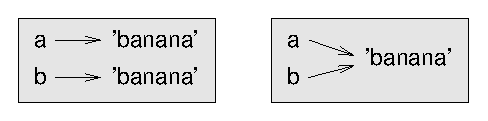
\includegraphics{figs/list1.eps}}
\afterfig

In one case, {\tt a} and {\tt b} refer to two different objects that
have the same value.  In the second case, they refer to the same
object.

\index{is operator}
\index{operator!is}

To check whether two variables refer to the same object, you can
use the {\tt is} operator.

\beforeverb
\begin{verbatim}
>>> a = 'banana'
>>> b = 'banana'
>>> a is b
True
\end{verbatim}
\afterverb
%
In this example, Python only created one string object,
and both {\tt a} and {\tt b} refer to it.

But when you create two lists, you get two objects:

\beforeverb
\begin{verbatim}
>>> a = [1, 2, 3]
>>> b = [1, 2, 3]
>>> a is b
False
\end{verbatim}
\afterverb
%
So the state diagram looks like this:

\index{state diagram}
\index{diagram!state}

\beforefig
\centerline{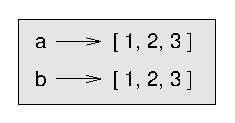
\includegraphics{figs/list2.eps}}
\afterfig

In this case we would say that the two lists are {\bf equivalent},
because they have the same elements, but not {\bf identical}, because
they are not the same object.  If two objects are identical, they are
also equivalent, but if they are equivalent, they are not necessarily
identical.

\index{equivalence}
\index{identity}

Until now, we have been using ``object'' and ``value''
interchangeably, but it is more precise to say that an object has a
value.  If you execute {\tt a = [1,2,3]}, {\tt a} refers to a list
object whose value is a particular sequence of elements.  If another
list has the same elements, we would say it has the same value.

\index{object}
\index{value}


\section{Aliasing}

\index{aliasing}
\index{reference!aliasing}

If {\tt a} refers to an object and you assign {\tt b = a},
then both variables refer to the same object:

\beforeverb
\begin{verbatim}
>>> a = [1, 2, 3]
>>> b = a
>>> b is a
True
\end{verbatim}
\afterverb
%
The state diagram looks like this:

\index{state diagram}
\index{diagram!state}

\beforefig
\centerline{
\includegraphics{figs/list3.eps}}
\afterfig

The association of a variable with an object is called a {\bf
reference}.  In this example, there are two references to the same
object.

\index{reference}

An object with more than one reference has more
than one name, so we say that the object is {\bf aliased}.

\index{mutability}

If the aliased object is mutable, 
changes made with one alias affect
the other:

\beforeverb
\begin{verbatim}
>>> b[0] = 17
>>> print a
[17, 2, 3]
\end{verbatim}
\afterverb
%
Although this behavior can be useful, it is error-prone.  In general,
it is safer to avoid aliasing when you are working with mutable
objects.

\index{immutability}

For immutable objects like strings, aliasing is not as much of a
problem.  In this example:

\beforeverb
\begin{verbatim}
a = 'banana'
b = 'banana'
\end{verbatim}
\afterverb
%
It almost never makes a difference whether {\tt a} and {\tt b} refer
to the same string or not.


\section{List arguments}

\index{list!as argument}
\index{argument}
\index{argument!list}
\index{reference}
\index{parameter}

When you pass a list to a function, the function gets a reference
to the list.
If the function modifies a list parameter, the caller sees the change.
For example, \verb"delete_head" removes the first element from a list:

\beforeverb
\begin{verbatim}
def delete_head(t):
    del t[0]
\end{verbatim}
\afterverb
%
Here's how it is used:

\beforeverb
\begin{verbatim}
>>> letters = ['a', 'b', 'c']
>>> delete_head(letters)
>>> print letters
['b', 'c']
\end{verbatim}
\afterverb
%
The parameter {\tt t} and the variable {\tt letters} are
aliases for the same object.  The stack diagram looks like
this:

\index{stack diagram}
\index{diagram!stack}

\beforefig
\centerline{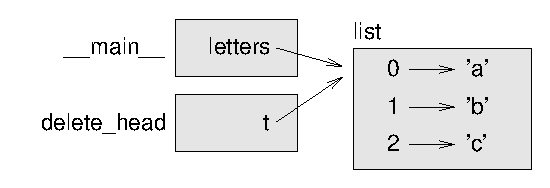
\includegraphics{figs/stack5.eps}}
\afterfig

Since the list is shared by two frames, I drew
it between them.

It is important to distinguish between operations that
modify lists and operations that create new lists.  For
example, the {\tt append} method modifies a list, but the
{\tt +} operator creates a new list:

\index{append method}
\index{method!append}
\index{list!concatenation}
\index{concatenation!list}

\beforeverb
\begin{verbatim}
>>> t1 = [1, 2]
>>> t2 = t1.append(3)
>>> print t1
[1, 2, 3]
>>> print t2
None

>>> t3 = t1 + [3]
>>> print t3
[1, 2, 3]
>>> t2 is t3
False
\end{verbatim}
\afterverb

This difference is important when you write functions that
are supposed to modify lists.  For example, this function
\emph{does not} delete the head of a list:

\beforeverb
\begin{verbatim}
def bad_delete_head(t):
    t = t[1:]              # WRONG!
\end{verbatim}
\afterverb

The slice operator creates a new list and the assignment
makes {\tt t} refer to it, but none of that has any effect
on the list that was passed as an argument.

\index{slice operator}
\index{operator!slice}

An alternative is to write a function that creates and
returns a new list.  For
example, {\tt tail} returns all but the first
element of a list:

\beforeverb
\begin{verbatim}
def tail(t):
    return t[1:]
\end{verbatim}
\afterverb
%
This function leaves the original list unmodified.
Here's how it is used:

\beforeverb
\begin{verbatim}
>>> letters = ['a', 'b', 'c']
>>> rest = tail(letters)
>>> print rest
['b', 'c']
\end{verbatim}
\afterverb


\begin{ex}

Write a function called {\tt chop} that takes a list and modifies
it, removing the first and last elements, and returns {\tt None}.

Then write a function called {\tt middle} that takes a list and
returns a new list that contains all but the first and last
elements.

\end{ex}


\section{Debugging}
\index{debugging}

Careless use of lists (and other mutable objects)
can lead to long hours of debugging.  Here are some common
pitfalls and ways to avoid them:

\begin{enumerate}

\item Don't forget that most list methods modify the argument and
  return {\tt None}.  This is the opposite of the string methods,
  which return a new string and leave the original alone.

If you are used to writing string code like this:

\beforeverb
\begin{verbatim}
word = word.strip()
\end{verbatim}
\afterverb

It is tempting to write list code like this:

\beforeverb
\begin{verbatim}
t = t.sort()           # WRONG!
\end{verbatim}
\afterverb

\index{sort method}
\index{method!sort}

Because {\tt sort} returns {\tt None}, the
next operation you perform with {\tt t} is likely to fail.

Before using list methods and operators, you should read the
documentation carefully and then test them in interactive mode.  The
methods and operators that lists share with other sequences (like
strings) are documented at
\url{docs.python.org/lib/typesseq.html}.  The
methods and operators that only apply to mutable sequences
are documented at \url{docs.python.org/lib/typesseq-mutable.html}.


\item Pick an idiom and stick with it.

Part of the problem with lists is that there are too many
ways to do things.  For example, to remove an element from
a list, you can use {\tt pop}, {\tt remove}, {\tt del},
or even a slice assignment.

To add an element, you can use the {\tt append} method or
the {\tt +} operator.  But don't forget that these are right: 

\beforeverb
\begin{verbatim}
t.append(x)
t = t + [x]
\end{verbatim}
\afterverb

And these are wrong:

\beforeverb
\begin{verbatim}
t.append([x])          # WRONG!
t = t.append(x)        # WRONG!
t + [x]                # WRONG!
t = t + x              # WRONG!
\end{verbatim}
\afterverb

Try out each of these examples in interactive mode to make sure
you understand what they do.  Notice that only the last
one causes a runtime error; the other three are legal, but they
do the wrong thing.


\item Make copies to avoid aliasing.

\index{aliasing!copying to avoid}
\index{copy!to avoid aliasing}

If you want to use a method like {\tt sort} that modifies
the argument, but you need to keep the original list as
well, you can make a copy.

\beforeverb
\begin{verbatim}
orig = t[:]
t.sort()
\end{verbatim}
\afterverb

In this example you could also use the built-in function {\tt sorted},
which returns a new, sorted list and leaves the original alone.
But in that case you should avoid using {\tt sorted} as a variable
name!

\item Lists, {\tt split}, and files

When we read and parse files, there are many opportunities
to encounter input that can crash our program so it is a good 
idea to revisit the {\bf guardian} pattern when it comes
writing programs that read through a file 
and look for a ``needle in the haystack''.

Lets revisit our program that is looking for the day of the
week on the from lines of our file.:

{\tt
From stephen.marquard@uct.ac.za {\bf Sat} Jan  5 09:14:16 2008
}

Since we are breaking this line into words, we could dispense
with the use of {\tt startswith} and simply look at the 
first word of the line to determine if we are interested
in the line at all.  We can use {\tt continue} to skip lines
that don't have ``From'' as the first word as follows:

\beforeverb
\begin{verbatim}
fhand = open('mbox-short.txt')
for line in fhand:
    words = line.split()
    if words[0] != 'From' : continue
    print words[2]
\end{verbatim}
\afterverb
%
This looks much simpler and we don't even need to do the 
{\tt rstrip} to remove the newline at the end of the file.
But is it better?

\beforeverb
\begin{verbatim}
python search8.py 
Sat
Traceback (most recent call last):
  File "search8.py", line 5, in <module>
    if words[0] != 'From' : continue
IndexError: list index out of range
\end{verbatim}
\afterverb
%
It kind of works and we see the day from the first line
(Sat) but then the program fails with a traceback error.
What went wrong?  What messed-up data caused our elegant, 
clever and very Pythonic program to fail?

You could stare at it for a long time and puzzle through
it or ask someone for help, but the quicker and smarter
approach is to add a {\tt print} statement.  The best place
to add the print statement is right before the line where
the program failed and print out the data that seems to be causing
the failure.

Now this approach may generate a lot of lines of output but at 
least you will immediately have some clue as to the 
problem at hand.  So we add a print of the variable
{\tt words} right before line five.  We even 
add a prefix ``Debug:'' to the line so we can keep
our regular output separate from our debug output.

\beforeverb
\begin{verbatim}
for line in fhand:
    words = line.split()
    print 'Debug:', words
    if words[0] != 'From' : continue
    print words[2]
\end{verbatim}
\afterverb
%
When we run the program, a lot of output scrolls off the screen
but at the end, we see our debug output and the traceback so 
we know what happened just before the traceback.

\beforeverb
\begin{verbatim}
Debug: ['X-DSPAM-Confidence:', '0.8475']
Debug: ['X-DSPAM-Probability:', '0.0000']
Debug: []
Traceback (most recent call last):
  File "search9.py", line 6, in <module>
    if words[0] != 'From' : continue
IndexError: list index out of range
\end{verbatim}
\afterverb
%
Each debug line is printing the list of words which we get
when we {\tt split} the line into words.  When the program fails
the list of words is empty \verb"[]".  If we open the file in a text editor
and look at the file, at that point it looks as follows:

\beforeverb
\begin{verbatim}
X-DSPAM-Result: Innocent
X-DSPAM-Processed: Sat Jan  5 09:14:16 2008
X-DSPAM-Confidence: 0.8475
X-DSPAM-Probability: 0.0000

Details: http://source.sakaiproject.org/viewsvn/?view=rev&rev=39772
\end{verbatim}
\afterverb
%
The error occurs when our program encounters a blank line! Of course there
are ``zero words'' on a blank line.  Why didn't we think of that 
when we were writing the code.  When the code looks for the first
word (\verb"word[0]") to check to see if it matches ``From'', 
we get an ``index out of range'' error.

This of course is the perfect place to add some {\bf guardian} code 
to avoid checking the first word if the first word is not there.
There are many ways to protect this code, we will choose to 
check the number of words we have before we look at the first word:

\beforeverb
\begin{verbatim}
fhand = open('mbox-short.txt')
count = 0
for line in fhand:
    words = line.split()
    # print 'Debug:', words
    if len(words) == 0 : continue
    if words[0] != 'From' : continue
    print words[2]
\end{verbatim}
\afterverb
%
First we commented out the debug print statement instead of removing it 
in case our modification fails and we need to debug again.  Then we added
a guardian statement that checks to see if we have zero words, and if so, 
we use {\tt continue} to skip to the next line in the file.

We can think of the two {\tt continue} statements as helping us refine
the set of lines which are ``interesting'' to us and which we want 
to process some more.  A line which has no words is ``uninteresting'' to 
us so we skip to the next line.  A line which does not have ``From''
as its first word is uninteresting to us so we skip it.

The program as modified runs successfully so perhaps it is correct.  Our
guardian statement does make sure that the {\tt words[0]} will never fail, 
but perhaps it is not enough.  When we are programming, we must always be 
thinking, ``What might go wrong?''.

\begin{ex}
Figure out which line of the above program is still not properly guarded.
See if you can construct a text file which causes the program to fail
and then modify the program so that the line is properly guarded and 
test it to make sure it handles your new text file.
\end{ex}

\begin{ex}
Rewrite the guardian code in the above example without two
{\tt if} statements.  Instead use a compound logical expression using the
{\tt and} logical operator with a single {\tt if} statement.
\end{ex}


\end{enumerate}



\section{Glossary}

\begin{description}

\item[aliasing:] A circumstance where two or more variables refer to the same
object.
\index{aliasing}

\item[delimiter:] A character or string used to indicate where a
string should be split.
\index{delimiter}

\item[element:] One of the values in a list (or other sequence),
also called items.
\index{element}

\item[equivalent:] Having the same value.
\index{equivalent}

\item[index:] An integer value that indicates an element in a list.
\index{index}

\item[identical:] Being the same object (which implies equivalence).
\index{identical}

\item[list:] A sequence of values.
\index{list}

\item[list traversal:] The sequential accessing of each element in a list.
\index{list!traversal}

\item[nested list:] A list that is an element of another list.
\index{nested list}

\item[object:] Something a variable can refer to.  An object
has a type and a value.
\index{object}

\item[reference:] The association between a variable and its value.
\index{reference}

\end{description}


\section{Exercises}

\begin{ex}
Download a copy of the file from 
\url{www.py4inf.com/code/romeo.txt}

Write a program to open the file {\tt romeo.txt} and read it
line by line.  For each line, split the line into  a list of 
words using the {\tt split} function.

For each word, check to see if the word is already in a list.  
If the word is not in the list, add it to the list.  

When the program completes, sort and print the resulting words
in alphabetical order.

\begin{verbatim}
Enter file: romeo.txt
['Arise', 'But', 'It', 'Juliet', 'Who', 'already', 
'and', 'breaks', 'east', 'envious', 'fair', 'grief', 
'is', 'kill', 'light', 'moon', 'pale', 'sick', 'soft', 
'sun', 'the', 'through', 'what', 'window', 
'with', 'yonder']
\end{verbatim}
\end{ex}

\begin{ex}
Write a program to read through the mail box data and when you find 
line that starts with ``From'', you will split the line into 
words using the {\tt split} function. We are interested in 
who sent the message which is the second word on the From line.

{\tt From stephen.marquard@uct.ac.za Sat Jan  5 09:14:16 2008 }

You will parse the From line and print out the second word for 
each From line and then you will also count the number of 
From (not From:) lines and print out a count at the end.

This is a sample good output with a few lines removed:

\beforeverb
\begin{verbatim}
python fromcount.py 
Enter a file name: mbox-short.txt
stephen.marquard@uct.ac.za
louis@media.berkeley.edu
zqian@umich.edu

[...some output removed...]

ray@media.berkeley.edu
cwen@iupui.edu
cwen@iupui.edu
cwen@iupui.edu
There were 27 lines in the file with From as the first word
\end{verbatim}
\afterverb

\end{ex}


\chapter{Dictionaries}
\index{dictionary}

\index{dictionary}
\index{type!dict}
\index{key}
\index{key-value pair}
\index{index}

A {\bf dictionary} is like a list, but more general.  In a list,
the positions (a.k.a. indices) have to be integers; in a dictionary 
the indices can be (almost) any type.

You can think of a dictionary as a mapping between a set of indices
(which are called {\bf keys}) and a set of values.  Each key maps to a
value.  The association of a key and a value is called a {\bf
  key-value pair} or sometimes an {\bf item}.

As an example, we'll build a dictionary that maps from English
to Spanish words, so the keys and the values are all strings.

The function {\tt dict} creates a new dictionary with no items.
Because {\tt dict} is the name of a built-in function, you
should avoid using it as a variable name.

\index{dict function}
\index{function!dict}

\beforeverb
\begin{verbatim}
>>> eng2sp = dict()
>>> print eng2sp
{}
\end{verbatim}
\afterverb

The squiggly-brackets, \verb"{}", represent an empty dictionary.
To add items to the dictionary, you can use square brackets:

\index{squiggly bracket}
\index{bracket!squiggly}

\beforeverb
\begin{verbatim}
>>> eng2sp['one'] = 'uno'
\end{verbatim}
\afterverb
%
This line creates an item that maps from the key
{\tt 'one'} to the value \verb"'uno'".  If we print the
dictionary again, we see a key-value pair with a colon
between the key and value:

\beforeverb
\begin{verbatim}
>>> print eng2sp
{'one': 'uno'}
\end{verbatim}
\afterverb
%
This output format is also an input format.  For example,
you can create a new dictionary with three items:

\beforeverb
\begin{verbatim}
>>> eng2sp = {'one': 'uno', 'two': 'dos', 'three': 'tres'}
\end{verbatim}
\afterverb
%
But if you print {\tt eng2sp}, you might be surprised:

\beforeverb
\begin{verbatim}
>>> print eng2sp
{'one': 'uno', 'three': 'tres', 'two': 'dos'}
\end{verbatim}
\afterverb
%
The order of the key-value pairs is not the same.  In fact, if
you type the same example on your computer, you might get a
different result.  In general, the order of items in
a dictionary is unpredictable.

But that's not a problem because
the elements of a dictionary are never indexed with integer indices.
Instead, you use the keys to look up the corresponding values:

\beforeverb
\begin{verbatim}
>>> print eng2sp['two']
'dos'
\end{verbatim}
\afterverb
%
The key {\tt 'two'} always maps to the value \verb"'dos'" so the order
of the items doesn't matter.

If the key isn't in the dictionary, you get an exception:

\index{exception!KeyError}
\index{KeyError}

\beforeverb
\begin{verbatim}
>>> print eng2sp['four']
KeyError: 'four'
\end{verbatim}
\afterverb
%
The {\tt len} function works on dictionaries; it returns the
number of key-value pairs:

\index{len function}
\index{function!len}

\beforeverb
\begin{verbatim}
>>> len(eng2sp)
3
\end{verbatim}
\afterverb
%
The {\tt in} operator works on dictionaries; it tells you whether
something appears as a \emph{key} in the dictionary (appearing
as a value is not good enough).

\index{membership!dictionary}
\index{in operator}
\index{operator!in}

\beforeverb
\begin{verbatim}
>>> 'one' in eng2sp
True
>>> 'uno' in eng2sp
False
\end{verbatim}
\afterverb
%
To see whether something appears as a value in a dictionary, you
can use the method {\tt values}, which returns the values as
a list, and then use the {\tt in} operator:

\index{values method}
\index{method!values}

\beforeverb
\begin{verbatim}
>>> vals = eng2sp.values()
>>> 'uno' in vals
True
\end{verbatim}
\afterverb
%
The {\tt in} operator uses different algorithms for lists and
dictionaries.  For lists, it uses a search algorithm, as in
Section~\ref{find}.  As the list gets longer, the search time gets
longer in direct proportion.  For dictionaries, Python uses an
algorithm called a {\bf hashtable} that has a remarkable property; the
{\tt in} operator takes about the same amount of time no matter how
many items there are in a dictionary.  I won't explain 
why hash functions are so magical,
but you can read more about it at
\url{wikipedia.org/wiki/Hash_table}.

\index{hashtable}

\begin{ex}
\label{wordlist2}

\index{set membership}
\index{membership!set}

Write a function that reads the words in {\tt words.txt} and
stores them as keys in a dictionary.  It doesn't matter what the
values are.  Then you can use the {\tt in} operator
as a fast way to check whether a string is in
the dictionary.

\end{ex}


\section{Dictionary as a set of counters}
\label{histogram}

\index{counter}

Suppose you are given a string and you want to count how many
times each letter appears.  There are several ways you could do it:

\begin{enumerate}

\item You could create 26 variables, one for each letter of the
alphabet.  Then you could traverse the string and, for each
character, increment the corresponding counter, probably using
a chained conditional.

\item You could create a list with 26 elements.  Then you could
convert each character to a number (using the built-in function
{\tt ord}), use the number as an index into the list, and increment
the appropriate counter.

\item You could create a dictionary with characters as keys
and counters as the corresponding values.  The first time you
see a character, you would add an item to the dictionary.  After
that you would increment the value of an existing item.

\end{enumerate}

Each of these options performs the same computation, but each
of them implements that computation in a different way.

\index{implementation}

An {\bf implementation} is a way of performing a computation;
some implementations are better than others.  For example,
an advantage of the dictionary implementation is that we don't
have to know ahead of time which letters appear in the string
and we only have to make room for the letters that do appear.

Here is what the code might look like:

\beforeverb
\begin{verbatim}
def histogram(s):
    d = dict()
    for c in s:
        if c not in d:
            d[c] = 1
        else:
            d[c] = d[c] + 1
    return d
\end{verbatim}
\afterverb
%
The name of the function is {\bf histogram}, which is a statistical
term for a set of counters (or frequencies).  

\index{histogram}
\index{frequency}
\index{traversal}

The first line of the
function creates an empty dictionary.  The {\tt for} loop traverses
the string.  Each time through the loop, if the character {\tt c} is
not in the dictionary, we create a new item with key {\tt c} and the
initial value 1 (since we have seen this letter once).  If {\tt c} is
already in the dictionary we increment {\tt d[c]}.

\index{histogram}

Here's how it works:

\beforeverb
\begin{verbatim}
>>> h = histogram('brontosaurus')
>>> print h
{'a': 1, 'b': 1, 'o': 2, 'n': 1, 's': 2, 'r': 2, 'u': 2, 't': 1}
\end{verbatim}
\afterverb
%
The histogram indicates that the letters {\tt 'a'} and \verb"'b'"
appear once; \verb"'o'" appears twice, and so on.

\begin{ex}

\index{get method}
\index{method!get}

Dictionaries have a method called {\tt get} that takes a key
and a default value.  If the key appears in the dictionary,
{\tt get} returns the corresponding value; otherwise it returns
the default value.  For example:

\beforeverb
\begin{verbatim}
>>> h = histogram('a')
>>> print h
{'a': 1}
>>> h.get('a', 0)
1
>>> h.get('b', 0)
0
\end{verbatim}
\afterverb
%
Use {\tt get} to write {\tt histogram} more concisely.  You
should be able to eliminate the {\tt if} statement.
\end{ex}

\section{Dictionaries and files}

One of the common uses of a dictionary is to count the occurrence
of words in a file with some written text.  
Lets start with a very simple file of
words taken from the text of \emph{Romeo and Juliet}
thanks to 
\url{http://shakespeare.mit.edu/Tragedy/romeoandjuliet/romeo_juliet.2.2.html}.

For the first set of examples, we will use a shortened and simplified version
of the text with no punctuation.  Later we will work with the text of the 
scene with punctuation included.

\beforeverb
\begin{verbatim}
But soft what light through yonder window breaks
It is the east and Juliet is the sun
Arise fair sun and kill the envious moon
Who is already sick and pale with grief
\end{verbatim}
\afterverb
%
We will write a Python program to read through the lines of the file, 
break each line into a list of words, and then loop through each 
of the words in the line, and count each word using a dictionary.

\index{nested loops}
\index{loop!nested}
You will see that we have two {\tt for} loops.  The outer loop is reading the
lines of the file and the inner loop is iterating through each
of the words on that particular line.  This is an example
of a pattern called {\bf nested loops} because one of the loops
is the \emph{outer} loop and the other loop is the \emph{inner}
loop.  

Because the inner loop executes all of its iterations each time
the outer loop makes a single iteration, we think of the inner
loop as iterating ``more quickly'' and the outer loop as iterating 
more slowly.

The combination of the two nested loops ensures that we will count
every word on every line of the input file.

\beforeverb
\begin{verbatim}
fname = raw_input('Enter the file name: ')
try:
    fhand = open(fname)
except:
    print 'File cannot be opened:', fname
    exit()

counts = dict()
for line in fhand:
    words = line.split()
    for word in words:
        if word not in counts:
            counts[word] = 1
        else:
            counts[word] += 1

print counts
\end{verbatim}
\afterverb
%
When we run the program, we see a raw dump of all of the counts in unsorted
hash order.
(the {\tt romeo.txt} file is available at
\url{www.py4inf.com/code/romeo.txt})

\beforeverb
\begin{verbatim}
python count1.py 
Enter the file name: romeo.txt
{'and': 3, 'envious': 1, 'already': 1, 'fair': 1, 
'is': 3, 'through': 1, 'pale': 1, 'yonder': 1, 
'what': 1, 'sun': 2, 'Who': 1, 'But': 1, 'moon': 1, 
'window': 1, 'sick': 1, 'east': 1, 'breaks': 1, 
'grief': 1, 'with': 1, 'light': 1, 'It': 1, 'Arise': 1, 
'kill': 1, 'the': 3, 'soft': 1, 'Juliet': 1}
\end{verbatim}
\afterverb
%
It is a bit inconvenient to look through the dictionary to find the
most common words and their counts, so we need to add some more 
Python code to get us the output that will be more helpful.

\section{Looping and dictionaries}

\index{dictionary!looping with}
\index{looping!with dictionaries}
\index{traversal}

If you use a dictionary as the sequence 
in a {\tt for} statement, it traverses
the keys of the dictionary.  For example, \verb"print_hist"
prints each key and the corresponding value:

\beforeverb
\begin{verbatim}
def print_hist(h):
    for c in h:
        print c, h[c]
\end{verbatim}
\afterverb
%
Here's what the output looks like:

\beforeverb
\begin{verbatim}
>>> h = histogram('parrot')
>>> print_hist(h)
a 1
p 1
r 2
t 1
o 1
\end{verbatim}
\afterverb
%
Again, the keys are in no particular order.

\index{keys method}
\index{method!keys}
If you want to print the keys in alphabetical order, you first 
make a list of the keys in the dictionary using the 
{\tt keys} method available in dictionary objects,
and then sort that list
and loop through the sorted list, looking up each
key printing out key/value pairs in sorted order as follows
as follows:

\beforeverb
\begin{verbatim}
def print_sorted_hist(h):
    lst = h.keys()
    lst.sort()
    for c in lst:
        print c, h[c]
\end{verbatim}
\afterverb
%
Here's what the output looks like:

\beforeverb
\begin{verbatim}
>>> h = histogram('parrot')
>>> print_sorted_hist(h)
a 1
o 1
p 1
r 2
t 1
\end{verbatim}
\afterverb
%
So now the keys are in alphabetical order.

\section{Advanced text parsing}

In the above example using the file {\tt romeo.txt},
we made the file as simple as possible by removing 
any and all punctuation by hand.  The real text 
has lots of punctuation as shown below:

\beforeverb
\begin{verbatim}
But, soft! what light through yonder window breaks?
It is the east, and Juliet is the sun.
Arise, fair sun, and kill the envious moon,
Who is already sick and pale with grief,
\end{verbatim}
\afterverb
%
Since the Python {\tt split} function looks for spaces and
treats words as tokens separated by spaces, we would treat the
words ``soft!'' and ``soft'' as \emph{different} words and create
a separate dictionary entry for each word.

Also since the file has capitalization, we would treat
``who'' and ``Who'' as different words with different 
counts.

We can solve both these problems by using the string
methods {\tt lower}, {\tt punctuation}, and {\tt translate}.  The 
{\tt translate} is the most subtle of the methods.  
Here is the documentation for {\tt translate}:

\verb"string.translate(s, table[, deletechars])"

\emph{Delete all characters from s that are in deletechars (if present), 
and then translate the characters using table, which must 
be a 256-character string giving the translation for each 
character value, indexed by its ordinal. If table is None, 
then only the character deletion step is performed.}

We will not specify the {\tt table} but we will use 
the {\tt deletechars} parameter to delete all of the punctuation.
We will even let Python tell us the list of characters
that it considers ``punctuation'':

\beforeverb
\begin{verbatim}
>>> import string
>>> string.punctuation
'!"#$%&\'()*+,-./:;<=>?@[\\]^_`{|}~'
\end{verbatim}
\afterverb
%
We make the following modifications to our program:

\beforeverb
\begin{verbatim}
import string                                          # New Code

fname = raw_input('Enter the file name: ')
try:
    fhand = open(fname)
except:
    print 'File cannot be opened:', fname
    exit()

counts = dict()
for line in fhand:
    line = line.translate(None, string.punctuation)    # New Code
    line = line.lower()                                # New Code
    words = line.split()
    for word in words:
        if word not in counts:
            counts[word] = 1
        else:
            counts[word] += 1

print counts
\end{verbatim}
\afterverb
%
We use {\tt translate} to remove all punctuation and {\tt lower} to 
force the line to lowercase.  Otherwise the program is unchanged.
Note for Python 2.5 and earlier, {\tt translate} does not 
accept {\tt None} as the first parameter so use this code for the translate 
call:

\beforeverb
\begin{verbatim}
print a.translate(string.maketrans(' ',' '), string.punctuation
\end{verbatim}
\afterverb
%
Part of learning the ``Art of Python'' or ``Thinking Pythonically''
is realizing that Python
often has built-in capabilities for many common data-analysis
problems.  Over time, you will see enough example code and read
enough of the documentation to know where to look to see if someone
has already written something that makes your job much easier.

The following is an abbreviated version of the output:
\beforeverb
\begin{verbatim}
Enter the file name: romeo-full.txt
{'swearst': 1, 'all': 6, 'afeard': 1, 'leave': 2, 'these': 2, 
'kinsmen': 2, 'what': 11, 'thinkst': 1, 'love': 24, 'cloak': 1, 
a': 24, 'orchard': 2, 'light': 5, 'lovers': 2, 'romeo': 40, 
'maiden': 1, 'whiteupturned': 1, 'juliet': 32, 'gentleman': 1, 
'it': 22, 'leans': 1, 'canst': 1, 'having': 1, ...}
\end{verbatim}
\afterverb
%
Looking through this output is still unwieldy and we can use
Python to gives us exactly what we are looking for, but to do 
so, we need to learn about Python {\bf tuples}.  We
will pick up this example once we learn about tuples.

\section{Debugging}
\index{debugging}

As you work with bigger datasets it can become unwieldy to
debug by printing and checking data by hand.  Here are some
suggestions for debugging large datasets:

\begin{description}

\item[Scale down the input:] If possible, reduce the size of the
dataset.  For example if the program reads a text file, start with
just the first 10 lines, or with the smallest example you can find.
You can either edit the files themselves, or (better) modify the
program so it reads only the first {\tt n} lines.

If there is an error, you can reduce {\tt n} to the smallest
value that manifests the error, and then increase it gradually
as you find and correct errors.

\item[Check summaries and types:] Instead of printing and checking the
entire dataset, consider printing summaries of the data: for example,
the number of items in a dictionary or the total of a list of numbers.

A common cause of runtime errors is a value that is not the right
type.  For debugging this kind of error, it is often enough to print
the type of a value.

\item[Write self-checks:]  Sometimes you can write code to check
for errors automatically.  For example, if you are computing the
average of a list of numbers, you could check that the result is
not greater than the largest element in the list or less than
the smallest.  This is called a ``sanity check'' because it detects
results that are ``insane.''

\index{sanity check}
\index{consistency check}

Another kind of check compares the results of two different
computations to see if they are consistent.  This is called a
``consistency check.''

\item[Pretty print the output:] Formatting debugging output
can make it easier to spot an error.  

\end{description}

Again, time you spend building scaffolding can reduce
the time you spend debugging.

\index{scaffolding}

\section{Glossary}

\begin{description}

\item[dictionary:] A mapping from a set of keys to their
corresponding values.
\index{dictionary}

\item[hashtable:] The algorithm used to implement Python
dictionaries.
\index{hashtable}

\item[hash function:] A function used by a hashtable to compute the
location for a key.
\index{hash function}

\item[histogram:] A set of counters.
\index{histogram}

\item[implementation:] A way of performing a computation.
\index{implementation}

\item[item:] Another name for a key-value pair.
\index{item!dictionary}

\item[key:] An object that appears in a dictionary as the
first part of a key-value pair.
\index{key}

\item[key-value pair:] The representation of the mapping from
a key to a value.
\index{key-value pair}

\item[lookup:] A dictionary operation that takes a key and finds
the corresponding value.
\index{lookup}

\item[nested loops:] When there is one or more loops ``inside'' of 
another loop.  The inner loop runs to completion each time the outer
loop runs once.
\index{nested loops}
\index{loop!nested}

\item[value:] An object that appears in a dictionary as the
second part of a key-value pair.  This is more specific than
our previous use of the word ``value.''
\index{value}

\end{description}

\section{Exercises}

\begin{ex}
Write a program that categorizes each mail message by which 
day of the week the commit was done. To do this look for 
lines which start with ``From'', then look for the 
third word and then keep a running count of each of the 
days of the week. At the end of the program print out the 
contents of your dictionary (order does not matter).

\beforeverb
\begin{verbatim}
Sample Line:
From stephen.marquard@uct.ac.za Sat Jan  5 09:14:16 2008

Sample Execution:
python dow.py
Enter a file name: mbox-short.txt
{'Fri': 20, 'Thu': 6, 'Sat': 1}
\end{verbatim}
\afterverb
\end{ex}

\begin{ex}
Write a program to read through a mail log, and figure 
out who had the most messages in the file.  The program looks 
for ``From'' lines and takes the second parameter on those 
lines as the person who sent the mail.

The program creates a Python dictionary that maps 
the sender's address to the total number of messages for that person.

After all the data has been read the program looks 
through the dictionary using a maximum loop
 (see Section~\ref{maximumloop})
to find who has the most 
messages and how many messages the person has.

\beforeverb
\begin{verbatim}
Enter a file name: mbox-short.txt
cwen@iupui.edu 5

Enter a file name: mbox.txt
zqian@umich.edu 195
\end{verbatim}
\afterverb
\end{ex}

\begin{ex}
This program records the domain name (instead of the address) 
where the message was sent from instead of who the mail 
came from (i.e. the whole e-mail address). At the end 
of the program print out the contents of your dictionary. 

\beforeverb
\begin{verbatim}
python schoolcount.py
Enter a file name: mbox-short.txt
{'media.berkeley.edu': 4, 'uct.ac.za': 6, 'umich.edu': 7, 
'gmail.com': 1, 'caret.cam.ac.uk': 1, 'iupui.edu': 8}
\end{verbatim}
\afterverb
\end{ex}

\chapter{Tuples}
\label{tuplechap}

\section{Tuples are immutable}

\index{tuple}
\index{type!tuple}
\index{sequence}

A tuple is a sequence of values much like a list.  
The values stored in a tuple can be any type, and
they are indexed by integers.
The important difference is that tuples are {\bf immutable}.
Tuples are also {\bf comparable} and {\bf hashable} so we can 
sort lists of them and use tuples as key values in Python
dictionaries.

\index{mutability}
\index{hashable}
\index{comparable}
\index{immutability}

Syntactically, a tuple is a comma-separated list of values:

\beforeverb
\begin{verbatim}
>>> t = 'a', 'b', 'c', 'd', 'e'
\end{verbatim}
\afterverb
%
Although it is not necessary, it is common to enclose tuples in
parentheses to help use quickly identify tuples when we look at
Python code:

\index{parentheses!tuples in}

\beforeverb
\begin{verbatim}
>>> t = ('a', 'b', 'c', 'd', 'e')
\end{verbatim}
\afterverb
%
To create a tuple with a single element, you have to include the final
comma:

\index{singleton}
\index{tuple!singleton}

\beforeverb
\begin{verbatim}
>>> t1 = ('a',)
>>> type(t1)
<type 'tuple'>
\end{verbatim}
\afterverb
%
Without the comma Python treats \verb"('a')" as an expression 
with a string in parentheses that evaluates to a string:

\beforeverb
\begin{verbatim}
>>> t2 = ('a')
>>> type(t2)
<type 'str'>
\end{verbatim}
\afterverb
%
Another way to construct a tuple is the built-in function {\tt tuple}.
With no argument, it creates an empty tuple:

\index{tuple function}
\index{function!tuple}

\beforeverb
\begin{verbatim}
>>> t = tuple()
>>> print t
()
\end{verbatim}
\afterverb
%
If the argument is a sequence (string, list or tuple), the result
of the call to {\tt tuple}
is a tuple with the elements of the sequence:

\beforeverb
\begin{verbatim}
>>> t = tuple('lupins')
>>> print t
('l', 'u', 'p', 'i', 'n', 's')
\end{verbatim}
\afterverb
%
Because {\tt tuple} is the name of a constructor, you should
avoid using it as a variable name.

Most list operators also work on tuples.  The bracket operator
indexes an element:

\index{bracket operator}
\index{operator!bracket}

\beforeverb
\begin{verbatim}
>>> t = ('a', 'b', 'c', 'd', 'e')
>>> print t[0]
'a'
\end{verbatim}
\afterverb
%
And the slice operator selects a range of elements.

\index{slice operator}
\index{operator!slice}
\index{tuple!slice}
\index{slice!tuple}

\beforeverb
\begin{verbatim}
>>> print t[1:3]
('b', 'c')
\end{verbatim}
\afterverb
%
But if you try to modify one of the elements of the tuple, you get
an error:

\index{exception!TypeError}
\index{TypeError}
\index{item assignment}
\index{assignment!item}

\beforeverb
\begin{verbatim}
>>> t[0] = 'A'
TypeError: object doesn't support item assignment
\end{verbatim}
\afterverb
%
You can't modify the elements of a tuple, but you can replace
one tuple with another:

\beforeverb
\begin{verbatim}
>>> t = ('A',) + t[1:]
>>> print t
('A', 'b', 'c', 'd', 'e')
\end{verbatim}
\afterverb
%

\section{Comparing tuples}

\index{comparison!tuple}
\index{tuple!comparison}
\index{sort method}
\index{method!sort}

The comparison operators work with tuples and other sequences;
Python starts by comparing the first element from each
sequence.  If they are equal, it goes on to the next element,
and so on, until it finds elements that differ.  Subsequent
elements are not considered (even if they are really big).

\beforeverb
\begin{verbatim}
>>> (0, 1, 2) < (0, 3, 4)
True
>>> (0, 1, 2000000) < (0, 3, 4)
True
\end{verbatim}
\afterverb
%
The {\tt sort} function works the same way.  It sorts 
primarily by first element, but in the case of a tie, it sorts
by second element, and so on.  

This feature lends itself to a pattern called {\bf DSU} for 

\begin{description}

\item[Decorate] a sequence by building a list of tuples
with one or more sort keys preceding the elements from the sequence,

\item[Sort] the list of tuples uring the Python built-in {\tt sort}, and

\item[Undecorate] by extracting the sorted elements of the sequence.

\end{description}

\label{DSU}
\index{DSU pattern}
\index{pattern!DSU}
\index{decorate-sort-undecorate pattern}
\index{pattern!decorate-sort-undecorate}

For example, suppose you have a list of words and you want to
sort them from longest to shortest:

\beforeverb
\begin{verbatim}
def sort_by_length(words):
    t = list()
    for word in words:
       t.append((len(word), word))

    t.sort(reverse=True)

    res = list()
    for length, word in t:
        res.append(word)
    return res
\end{verbatim}
\afterverb
%
The first loop builds a list of tuples, where each
tuple is a word preceded by its length.

{\tt sort} compares the first element, length, first, and
only considers the second element to break ties.  The keyword argument
{\tt reverse=True} tells {\tt sort} to go in decreasing order.

\index{keyword argument}
\index{argument!keyword}
\index{traversal}

The second loop traverses the list of tuples and builds a list of
words in descending order of length.


\section{Tuple assignment}
\label{tuple assignment}

\index{tuple!assignment}
\index{assignment!tuple}
\index{swap pattern}
\index{pattern!swap}

One of the unique syntactic features of the Python language
is the ability to have a tuple on the left hand
side of an assignment statement.  This allows you to assign
more than one variable at a time when the left hand side is a 
sequence.

In this example we have a two element list (which is a sequence) and
assign the first and second elements of the sequence
to the variables {\tt x} and {\tt y} in a single statement.

\beforeverb
\begin{verbatim}
>>> m = [ 'have', 'fun' ]
>>> x, y = m
>>> x
'have'
>>> y
'fun'
>>> 
\end{verbatim}
\afterverb
%
It is not magic, Python \emph{roughly} translates the 
tuple assignment syntax
to be the following:\footnote{Python does not translate the 
syntax literally.  For example if you try this with a dictionary
it will not work as might expect.}

\beforeverb
\begin{verbatim}
>>> m = [ 'have', 'fun' ]
>>> x = m[0]
>>> y = m[1]
>>> x
'have'
>>> y
'fun'
>>> 
\end{verbatim}
\afterverb

Stylistically when we use a tuple on the left hand side of the assignment
statement, we omit the parentheses, but the following is an equally 
valid syntax:

\beforeverb
\begin{verbatim}
>>> m = [ 'have', 'fun' ]
>>> (x, y) = m
>>> x
'have'
>>> y
'fun'
>>> 
\end{verbatim}
\afterverb
%
A particularly clever application of tuple assignment allows
us to {\bf swap} the values of two variables in a single statement:

\beforeverb
\begin{verbatim}
>>> a, b = b, a
\end{verbatim}
\afterverb
%
Both sides of this statement are tuples, but
the left side is a tuple of variables; the right side is a tuple of
expressions.  Each value on the right side 
is assigned to its respective variable on the left side.  
All the expressions on the right side are evaluated before any
of the assignments.

The number of variables on the left and the number of
values on the right have to be the same:

\index{exception!ValueError}
\index{ValueError}

\beforeverb
\begin{verbatim}
>>> a, b = 1, 2, 3
ValueError: too many values to unpack
\end{verbatim}
\afterverb
%
More generally, the right side can be any kind of sequence
(string, list or tuple).  For example, to split an email address
into a user name and a domain, you could write:

\index{split method}
\index{method!split}
\index{email address}

\beforeverb
\begin{verbatim}
>>> addr = 'monty@python.org'
>>> uname, domain = addr.split('@')
\end{verbatim}
\afterverb
%
The return value from {\tt split} is a list with two elements;
the first element is assigned to {\tt uname}, the second to
{\tt domain}.

\beforeverb
\begin{verbatim}
>>> print uname
monty
>>> print domain
python.org
\end{verbatim}
\afterverb
%

\section{Dictionaries and tuples}

\index{dictionary}
\index{items method}
\index{method!items}
\index{key-value pair}

Dictionaries have a method called {\tt items} that returns a list of
tuples, where each tuple is a key-value 
pair\footnote{This behavior is slightly different in Python 3.0.}.

\beforeverb
\begin{verbatim}
>>> d = {'a':10, 'b':1, 'c':22}
>>> t = d.items()
>>> print t
[('a', 10), ('c', 22), ('b', 1)]
\end{verbatim}
\afterverb
%
As you should expect from a dictionary, the items are in no
particular order.

However, since the list of tuples is a list, and tuples are comparable,
we can now sort the list of tuples.  Converting a dictionary
to a list of tuples is a way for us to output the contents of a 
dictionary sorted by key:

\beforeverb
\begin{verbatim}
>>> d = {'a':10, 'b':1, 'c':22}
>>> t = d.items()
>>> t
[('a', 10), ('c', 22), ('b', 1)]
>>> t.sort()
>>> t
[('a', 10), ('b', 1), ('c', 22)]
\end{verbatim}
\afterverb
%
The new list is sorted in ascending alphabetical order by the key value.

\section{Multiple assignment with dictionaries}

\index{traverse!dictionary}
\index{dictionary!traversal}

Combining {\tt items}, tuple assignment and {\tt for}, you
can see a nice code pattern for traversing the keys and values of a dictionary
in a single loop:

\beforeverb
\begin{verbatim}
for key, val in d.items():
    print val, key
\end{verbatim}
\afterverb
%
This loop has two {\bf iteration variables} because {\tt items} returns
a list of tuples and {\tt key, val} is a tuple assignment
that successively iterates through each of the key/value pairs in the dictionary.  

For each iteration
through the loop, both {\tt key} and {\tt value} are advanced to the
next key/value pair in the dictionary (still in hash order).

The output of this loop is:

\beforeverb
\begin{verbatim}
0 a
2 c
1 b
\end{verbatim}
\afterverb
%
Again in hash key order (i.e. no particular order).

If we combine these two techniques, we can print out the contents
of a dictionary sorted by the \emph{value} stored in each key/value
pair.

To do this, we first make a list of tuples where each tuple is 
{\tt (value, key)}.  The {\tt items} method would give us a list of 
{\tt (key, value)} tuples--but this time we want to sort by value not key.
Once we have constructed the list with the value/key tuples, it is a simple
matter to sort the list in reverse order and print out the new, sorted list.

\beforeverb
\begin{verbatim}
>>> d = {'a':10, 'b':1, 'c':22}
>>> l = list()
>>> for key, val in d.items() :
...     l.append( (val, key) )
... 
>>> l
[(10, 'a'), (22, 'c'), (1, 'b')]
>>> l.sort(reverse=True)
>>> l
[(22, 'c'), (10, 'a'), (1, 'b')]
>>> 
\end{verbatim}
\afterverb
%
By hand-constructing the list of tuples to have the value as the first
element of each tuple, we can sort the list of tuples and get our dictionary
contents sorted by value.

\section{The most common words}

Coming back to our running example of the text from \emph{Romeo and Juliet} 
Act 2, Scene 2, we can augment our program to use this technique to 
print the ten most common words in the text as follows:

\beforeverb
\begin{verbatim}
import string
fhand = open('romeo-full.txt')
counts = dict()
for line in fhand:
    line = line.translate(None, string.punctuation)
    line = line.lower()
    words = line.split()
    for word in words:
        if word not in counts:
            counts[word] = 1
        else:
            counts[word] += 1

# Sort the dictionary by value
lst = list()
for key, val in counts.items():
    lst.append( (val, key) )

lst.sort(reverse=True)

for key, val in lst[:10] :
    print key, val
\end{verbatim}
\afterverb
%
The first part of the program which reads the file and computes 
the dictionary that maps each word to the count of words in the 
document is unchanged.  But instead of simply printing out 
{\tt counts} and ending the program, we construct a list 
of {\tt (val, key)} tuples and then sort the list in reverse order.

Since the value is first, it will be used for the comparisons and 
if there is more than one tuple with the same value, it will look
at the second element (the key) so tuples where the value is the
same will be further sorted by the alphabetical order of the key.

At the end we write a nice {\t for loop} which does a multiple
assignment iteration and prints out the ten most common words
by iterating through a slice of the list ({\tt lst[:10]}).

So now the output finally looks like what we want for our word 
frequency analysis.

\beforeverb
\begin{verbatim}
61 i
42 and
40 romeo
34 to
34 the
32 thou
32 juliet
30 that
29 my
24 thee
\end{verbatim}
\afterverb
%
The fact that this relatively complex data parsing and analysis 
can be done with a relatively easy-to-understand 19 line Python
program is one reason why Python is a good choice as a language 
for exploring information.

\section{Using tuples as keys in dictionaries}

\index{tuple!as key in dictionary}
\index{hashable}

Because tuples are {\bf hashable} and lists are not, if we want to 
create a {\bf composite} key to use in a dictionary we must use a tuple as
the key.

We would encounter a composite key if we wanted to create a 
telephone directory that maps
from last-name, first-name pairs to telephone numbers.  Assuming
that we have defined the variables 
{\tt last}, {\tt first} and {\tt number}, we could write
a dictionary assignment statement as follows:

\beforeverb
\begin{verbatim}
directory[last,first] = number
\end{verbatim}
\afterverb
%
The expression in brackets is a tuple.  We could use tuple
assignment in a {\tt for} loop to traverse this dictionary.

\index{tuple!in brackets}

\beforeverb
\begin{verbatim}
for last, first in directory:
    print first, last, directory[last,first]
\end{verbatim}
\afterverb
%
This loop traverses the keys in {\tt directory}, which are tuples.  It
assigns the elements of each tuple to {\tt last} and {\tt first}, then
prints the name and corresponding telephone number.

There are two ways to represent tuples in a state diagram.  The more
detailed version shows the indices and elements just as they appear in
a list.  For example, the tuple \verb"('Cleese', 'John')" would appear:

\index{state diagram}
\index{diagram!state}

\beforefig
\centerline{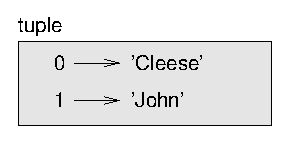
\includegraphics{figs/tuple1.eps}}
\afterfig

But in a larger diagram you might want to leave out the
details.  For example, a diagram of the telephone directory might
appear:

\beforefig
\centerline{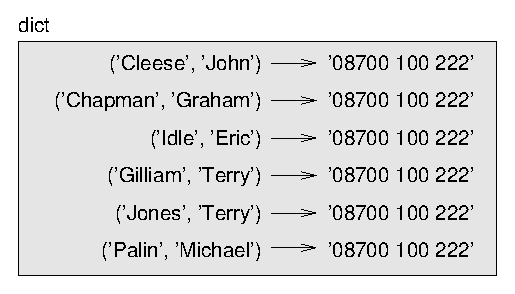
\includegraphics{figs/dict2.eps}}
\afterfig

Here the tuples are shown using Python syntax as a graphical
shorthand.

The telephone number in the diagram is the complaints line for the
BBC, so please don't call it.

\section{Sequences: strings, lists, and tuples--Oh My!}
\index{sequence}

I have focused on lists of tuples, but almost all of the examples in
this chapter also work with lists of lists, tuples of tuples, and
tuples of lists.  To avoid enumerating the possible combinations, it
is sometimes easier to talk about sequences of sequences.

In many contexts, the different kinds of sequences (strings, lists and
tuples) can be used interchangeably.  So how and why do you choose one
over the others?

\index{string}
\index{list}
\index{tuple}
\index{mutability}
\index{immutability}

To start with the obvious, strings are more limited than other
sequences because the elements have to be characters.  They are
also immutable.  If you need the ability to change the characters
in a string (as opposed to creating a new string), you might
want to use a list of characters instead.

Lists are more common than tuples, mostly because they are mutable.
But there are a few cases where you might prefer tuples:

\begin{enumerate}

\item In some contexts, like a {\tt return} statement, it is
syntactically simpler to create a tuple than a list.  In other
contexts, you might prefer a list.

\item If you want to use a sequence as a dictionary key, you
have to use an immutable type like a tuple or string.

\item If you are passing a sequence as an argument to a function,
using tuples reduces the potential for unexpected behavior
due to aliasing.

\end{enumerate}

Because tuples are immutable, they don't provide methods
like {\tt sort} and {\tt reverse}, which modify existing lists.
However Python provides the built-in functions {\tt sorted}
and {\tt reversed}, which take any sequence as a parameter
and return a new list with the same elements in a different
order.

\index{sorted function}
\index{function!sorted}
\index{reversed function}
\index{function!reversed}


\section{Debugging}

\index{debugging}
\index{data structure}
\index{shape error}
\index{error!shape}

Lists, dictionaries and tuples are known generically as {\bf data
  structures}; in this chapter we are starting to see compound data
structures, like lists of tuples, and dictionaries that contain tuples
as keys and lists as values.  Compound data structures are useful, but
they are prone to what I call {\bf shape errors}; that is, errors
caused when a data structure has the wrong type, size or composition
or perhaps you write some code and forget the shape of your data
and introduce an error.

For example, if you are expecting a list with one integer and I
give you a plain old integer (not in a list), it won't work.

When you are debugging a program, and especially if you are
working on a hard bug, there are four things to try:

\begin{description}

\item[reading:] Examine your code, read it back to yourself, and
check that it says what you meant to say.

\item[running:] Experiment by making changes and running different
versions.  Often if you display the right thing at the right place
in the program, the problem becomes obvious, but sometimes you have to
spend some time to build scaffolding.

\item[ruminating:] Take some time to think!  What kind of error
is it: syntax, runtime, semantic?  What information can you get from
the error messages, or from the output of the program?  What kind of
error could cause the problem you're seeing?  What did you change
last, before the problem appeared?

\item[retreating:] At some point, the best thing to do is back
off, undoing recent changes, until you get back to a program that
works and that you understand.  Then you can start rebuilding.

\end{description}

Beginning programmers sometimes get stuck on one of these activities
and forget the others.  Each activity comes with its own failure
mode.

\index{typographical error}

For example, reading your code might help if the problem is a
typographical error, but not if the problem is a conceptual
misunderstanding.  If you don't understand what your program does, you
can read it 100 times and never see the error, because the error is in
your head.

\index{experimental debugging}

Running experiments can help, especially if you run small, simple
tests.  But if you run experiments without thinking or reading your
code, you might fall into a pattern I call ``random walk programming,''
which is the process of making random changes until the program
does the right thing.  Needless to say, random walk programming
can take a long time.

\index{random walk programming}
\index{development plan!random walk programming}

You have to take time to think.  Debugging is like an
experimental science.  You should have at least one hypothesis about
what the problem is.  If there are two or more possibilities, try to
think of a test that would eliminate one of them.

Taking a break helps with the thinking.  So does talking.
If you explain the problem to someone else (or even yourself), you
will sometimes find the answer before you finish asking the question.

But even the best debugging techniques will fail if there are too many
errors, or if the code you are trying to fix is too big and
complicated.  Sometimes the best option is to retreat, simplifying the
program until you get to something that works and that you
understand.

Beginning programmers are often reluctant to retreat because
they can't stand to delete a line of code (even if it's wrong).
If it makes you feel better, copy your program into another file
before you start stripping it down.  Then you can paste the pieces
back in a little bit at a time.

Finding a hard bug requires reading, running, ruminating, and
sometimes retreating.  If you get stuck on one of these activities,
try the others.


\section{Glossary}

\begin{description}

\item[comparable:] A type where one value can be checked to see if it is
greater than, less than or equal to another value of the same type.
Types which are comparable can be put in a list and sorted.
\index{comparable}

\item[data structure:] A collection of related values, often
organized in lists, dictionaries, tuples, etc.
\index{data structure}

\item[DSU:] Abbreviation of ``decorate-sort-undecorate,'' a
pattern that involves building a list of tuples, sorting, and
extracting part of the result.
\index{DSU pattern}

\item[gather:] The operation of assembling a variable-length
argument tuple.
\index{gather}

\item[hashable:] A type that has a hash function.  Immutable
types like integers,
floats and strings are hashable; mutable types like lists and
dictionaries are not.
\index{hashable}

\item[scatter:] The operation of treating a sequence as a list of
arguments.
\index{scatter}

\item[shape (of a data structure):] A summary of the type,
size and composition of a data structure.
\index{shape}

\item[singleton:] A list (or other sequence) with a single element.
\index{singleton}

\item[tuple:] An immutable sequence of elements.
\index{tuple}

\item[tuple assignment:] An assignment with a sequence on the
right side and a tuple of variables on the left.  The right
side is evaluated and then its elements are assigned to the
variables on the left.
\index{tuple assignment}
\index{assignment!tuple}

\end{description}


\section{Exercises}

\begin{ex}
Revise a previous program as follows:  Read and 
parse the ``From'' lines and pull out the 
addresses from the line.   Count the number of
messages from each person using a dictionary.

After all the data has been read print 
the person with the most commits by creating
a list of (count, email) tuples from the 
dictionary and then sorting the list in reverse
order and print out the person who has the most
commits.

\beforeverb
\begin{verbatim}
Sample Line:
From stephen.marquard@uct.ac.za Sat Jan  5 09:14:16 2008

Enter a file name: mbox-short.txt
cwen@iupui.edu 5

Enter a file name: mbox.txt
zqian@umich.edu 195
\end{verbatim}
\afterverb
\end{ex}
\begin{ex}
This program counts the distribution of the hour of the day for 
each of the messages. You can pull the hour from the ``From'' 
line by finding the time string and then splitting that string 
into parts using the colon character. Once you have accumulated 
the counts for each hour, print out the counts, one per line, 
sorted by hour as shown below. 
\beforeverb
\begin{verbatim}
Sample Execution:
python timeofday.py
Enter a file name: mbox-short.txt
04 3
06 1
07 1
09 2
10 3
11 6
14 1
15 2
16 4
17 2
18 1
19 1
\end{verbatim}
\afterverb
\end{ex}


\begin{ex}
Write a function called \verb"most_frequent" that takes a string and
prints the letters in decreasing order of frequency.  Find text
samples from several different languages and see how letter frequency
varies between languages.  Compare your results with the tables at
\url{wikipedia.org/wiki/Letter_frequencies}.

\index{letter frequency}
\index{frequency!letter}

\end{ex}

\chapter{Automating common tasks on your computer}

Up to now, we have focused on writing programs that read the 
data in a single file.  Python can also 
read data from a network, database, or even look through all the
folders on your computer.  

In this chapter, we will write programs that scan 
scan through your computer and 
perform some operation on each file.  
Files are organized into directories (also called ``folders'').
Simple Python scripts
can make short work of simple tasks that must be done to 
hundreds or thousands of files
spread across a directory tree or your entire computer.

To walk through all the directories and files in a tree we use 
{\tt os.walk} and a {\tt for} loop.  This is similar to how 
{\tt open} allows us to write a loop to read the contents of a file,
{\tt socket} allows us to write a loop to read the contents of a network connection, and
{\tt urllib} allows us to open a web document and loop through its contents.

\section{File names and paths}
\label{paths}

\index{file name}
\index{path}
\index{directory}
\index{folder}

Every running program has a ``current directory,'' which is the
default directory for most operations.  
For example, when you open a file for reading, Python looks for it in the
current directory.

\index{os module}
\index{module!os}

The {\tt os} module provides functions for working with files and
directories ({\tt os} stands for ``operating system'').  {\tt os.getcwd}
returns the name of the current directory:

\index{getcwd function}
\index{function!getcwd}

\beforeverb
\begin{verbatim}
>>> import os
>>> cwd = os.getcwd()
>>> print cwd
/home/dinsdale
\end{verbatim}
\afterverb
%
{\tt cwd} stands for {\bf current working directory}.  The result in
this example is {\tt /home/dinsdale}, which is the home directory of a
user named {\tt dinsdale}.

\index{working directory}
\index{directory!working}

A string like {\tt cwd} that identifies a file is called a path.
A {\bf relative path} starts from the current directory;
an {\bf absolute path} starts from the topmost directory in the
file system.

\index{relative path}
\index{path!relative}
\index{absolute path}
\index{path!absolute}

The paths we have seen so far are simple file names, so they are
relative to the current directory.  To find the absolute path to
a file, you can use {\tt os.path.abspath}:

\beforeverb
\begin{verbatim}
>>> os.path.abspath('memo.txt')
'/home/dinsdale/memo.txt'
\end{verbatim}
\afterverb
%
{\tt os.path.exists} checks
whether a file or directory exists:

\index{exists function}
\index{function!exists}

\beforeverb
\begin{verbatim}
>>> os.path.exists('memo.txt')
True
\end{verbatim}
\afterverb
%
If it exists, {\tt os.path.isdir} checks whether it's a directory:

\beforeverb
\begin{verbatim}
>>> os.path.isdir('memo.txt')
False
>>> os.path.isdir('music')
True
\end{verbatim}
\afterverb
%
Similarly, {\tt os.path.isfile} checks whether it's a file.

{\tt os.listdir} returns a list of the files (and other directories)
in the given directory:

\beforeverb
\begin{verbatim}
>>> os.listdir(cwd)
['music', 'photos', 'memo.txt']
\end{verbatim}
\afterverb
%


\section{Example: Cleaning up a photo directory}

Some time ago, I built a bit of Flickr-like software that 
received photos from my cellphone and stored those photos
on my server.  I wrote this before Flickr existed and kept 
using it after Flickr existed because
I wanted to keep original copies of my images forever.

I would also send a simple one-line text description in the MMS message
or the subject line of the E-Mail message.  I stored these messages
in a text file in the same directory as the image file.   I came up 
with a directory structure based on the month, year, day and time the 
photo was taken.   The following would be an example of the naming for 
one photo and its existing description:

\beforeverb
\begin{verbatim}
./2006/03/24-03-06_2018002.jpg
./2006/03/24-03-06_2018002.txt
\end{verbatim}
\afterverb
%
After seven years, I had a lot of photos and captions.  Over the years
as I switched cell phones, sometimes my code to extract the caption from the message 
would break and add a bunch of useless data on my server instead of a caption.  

I wanted to go through these files and figure out which of the 
text files were really captions and which were junk and then delete the bad
files.  The first thing to do was to get a simple inventory of 
how many text files I had in of the sub-folders
using the following program:

\beforeverb
\begin{verbatim}
import os
count = 0
for (dirname, dirs, files) in os.walk('.'):
   for filename in files:
       if filename.endswith('.txt') :
           count = count + 1
print 'Files:', count

python txtcount.py
Files: 1917
\end{verbatim}
\afterverb
%
The key bit of code that makes this possible is the {\tt os.walk}
library in Python.  When we call {\tt os.walk} and give it a starting
directory, it will ``walk'' through all of the directories 
and sub-directories recursively.   The string ``.'' indicates
to start in the current directory and walk downward.
As it encounters each directory,
we get three values in a tuple in the body of the {\tt for} loop.  
The first value is the current
directory name, the second value is the list of sub-directories 
in the current directory, and the third value is a list of files
in the current directory.

We do not have to explicitly look into each of the sub-directories
because we can count on {\tt os.walk} to visit every 
folder eventually.  But we do want to look at each file, so 
we write a simple {\tt for} loop to examine each of the files 
in the current directory.   We check each file to see if 
it ends with ``.txt'' and then count the number of 
files through the whole directory tree that end with the
suffix ``.txt''.

Once we have a sense of how many files end with ``.txt'', the next
thing to do is try to automatically
determine in Python which files are bad and which files
are good.   So we write a simple program to print out the
files and the size of each file:

\beforeverb
\begin{verbatim}
import os
from os.path import join
for (dirname, dirs, files) in os.walk('.'):
   for filename in files:
       if filename.endswith('.txt') :
           thefile = os.path.join(dirname,filename)
           print os.path.getsize(thefile), thefile
\end{verbatim}
\afterverb
%
Now instead of just counting the files, we create 
a file name by concatenating the directory name with
the name of the file within the directory using
{\tt os.path.join}.   It is important to use 
{\tt os.path.join} instead of string concatenation 
because on Windows we use a backslash
(\verb"\") to construct file paths and on Linux
or Apple we use a forward slash (\verb"/") 
to construct file paths.  The {\tt os.path.join}
knows these differences and knows what system
we are running on and it does the proper concatenation
depending on the system.  So the same Python code
runs on either Windows or UNIX-style systems.

Once we have the full file name with directory
path, we use the {\tt os.path.getsize} utility
to get the size and print it out, producing the 
following output:

\beforeverb
\begin{verbatim}
python txtsize.py
...
18 ./2006/03/24-03-06_2303002.txt
22 ./2006/03/25-03-06_1340001.txt
22 ./2006/03/25-03-06_2034001.txt
...
2565 ./2005/09/28-09-05_1043004.txt
2565 ./2005/09/28-09-05_1141002.txt
...
2578 ./2006/03/27-03-06_1618001.txt
2578 ./2006/03/28-03-06_2109001.txt
2578 ./2006/03/29-03-06_1355001.txt
...
\end{verbatim}
\afterverb
%
Scanning the output, we notice that some files are pretty short and 
a lot of the files are pretty large and the same size (2578 and 2565). 
When we take a look at a few of these larger files by hand, 
it looks like the large 
files are nothing but a generic bit of identical HTML that came 
in from mail sent to my system from my T-Mobile phone:

\beforeverb
\begin{verbatim}
<html>
        <head>
                <title>T-Mobile</title>
...
\end{verbatim}
\afterverb
%
Skimming through the file, it looks like there is no good information
in these files so we can probably delete them.

But before we delete the files, we will write a program to look for files
that are more than one line long and show the contents of the file.
But let's not bother showing ourselves those files that are exactly
2578 or 2565 characters long since we know that these files have no useful
information.

So we write the following program:
\beforeverb
\begin{verbatim}
import os
from os.path import join
for (dirname, dirs, files) in os.walk('.'):
   for filename in files:
       if filename.endswith('.txt') :
           thefile = os.path.join(dirname,filename)
           size = os.path.getsize(thefile)
           if size == 2578 or size == 2565:
               continue
           fhand = open(thefile,'r')
           lines = list()
           for line in fhand:
               lines.append(line)
           fhand.close()
           if len(lines) > 1:
                print len(lines), thefile
                print lines[:4]
\end{verbatim}
\afterverb
%
We use a {\tt continue} to skip files with the two 
``bad sizes'', then open the rest of the files
and read the lines of the file into a Python list
and if the file has more than one line we print
out how many lines are in the file and print out
the first three lines.

It looks like filtering out those two bad file sizes, and assuming
that all one-line files are correct, we are down to some pretty clean
data:

\beforeverb
\begin{verbatim}
python txtcheck.py 
3 ./2004/03/22-03-04_2015.txt
['Little horse rider\r\n', '\r\n', '\r']
2 ./2004/11/30-11-04_1834001.txt
['Testing 123.\n', '\n']
3 ./2007/09/15-09-07_074202_03.txt
['\r\n', '\r\n', 'Sent from my iPhone\r\n']
3 ./2007/09/19-09-07_124857_01.txt
['\r\n', '\r\n', 'Sent from my iPhone\r\n']
3 ./2007/09/20-09-07_115617_01.txt
...
\end{verbatim}
\afterverb
%
But there is one more annoying pattern of files: 
there are some three-line files that consist of
two blank lines followed by a line that says
``Sent from my iPhone'' that have slipped 
into my data.   So we make the following change
to the program to deal with these files as well.

\beforeverb
\begin{verbatim}
           lines = list()
           for line in fhand:
               lines.append(line)
           if len(lines) == 3 and lines[2].startswith('Sent from my iPhone') :
               continue
           if len(lines) > 1:
                print len(lines), thefile
                print lines[:4]
\end{verbatim}
\afterverb
%
We simply check if we have a three-line file, and if the third 
line starts with the specified text, we skip it.

Now when we run the program, we only see four remaining 
multi-line files and all of those files look pretty reasonable:
\beforeverb
\begin{verbatim}
python txtcheck2.py 
3 ./2004/03/22-03-04_2015.txt
['Little horse rider\r\n', '\r\n', '\r']
2 ./2004/11/30-11-04_1834001.txt
['Testing 123.\n', '\n']
2 ./2006/03/17-03-06_1806001.txt
['On the road again...\r\n', '\r\n']
2 ./2006/03/24-03-06_1740001.txt
['On the road again...\r\n', '\r\n']
\end{verbatim}
\afterverb
%
If you look at the overall pattern of this program,
we have successively refined how we accept or reject
files and once we found a pattern that was ``bad'' we used
{\tt continue} to skip the bad files so we could refine
our code to find more file patterns that were bad.

Now we are getting ready to delete the files, so 
we are going to flip the logic and instead of printing out 
the remaining good files, we will print out the ``bad''
files that we are about to delete.
\beforeverb
\begin{verbatim}
import os
from os.path import join
for (dirname, dirs, files) in os.walk('.'):
   for filename in files:
       if filename.endswith('.txt') :
           thefile = os.path.join(dirname,filename)
           size = os.path.getsize(thefile)
           if size == 2578 or size == 2565:
               print 'T-Mobile:',thefile
               continue
           fhand = open(thefile,'r')
           lines = list()
           for line in fhand:
               lines.append(line)
           fhand.close()
           if len(lines) == 3 and lines[2].startswith('Sent from my iPhone') :
               print 'iPhone:', thefile
               continue
\end{verbatim}
\afterverb
%
We can now see a list of candidate files that we are about
to delete and why these files are up for deleting.
The program produces the following output:
\beforeverb
\begin{verbatim}
python txtcheck3.py
...
T-Mobile: ./2006/05/31-05-06_1540001.txt
T-Mobile: ./2006/05/31-05-06_1648001.txt
iPhone: ./2007/09/15-09-07_074202_03.txt
iPhone: ./2007/09/15-09-07_144641_01.txt
iPhone: ./2007/09/19-09-07_124857_01.txt
...
\end{verbatim}
\afterverb
%
We can spot-check these files to make sure that we did not inadvertently
end up introducing a bug in our program or perhaps our logic 
caught some files we did not want to catch.

Once we are satisfied that this is the list of files we want to delete,
we make the following change to the program:
\beforeverb
\begin{verbatim}
           if size == 2578 or size == 2565:
               print 'T-Mobile:',thefile
               os.remove(thefile)
               continue
...
           if len(lines) == 3 and lines[2].startswith('Sent from my iPhone') :
               print 'iPhone:', thefile
               os.remove(thefile)
               continue
\end{verbatim}
\afterverb
%
In this version of the program, we will both print the file out 
and remove the bad files
using {\tt os.remove}.

\beforeverb
\begin{verbatim}
python txtdelete.py 
T-Mobile: ./2005/01/02-01-05_1356001.txt
T-Mobile: ./2005/01/02-01-05_1858001.txt
...
\end{verbatim}
\afterverb
%
Just for fun, run the program a second time and it will produce no output
since the bad files are already gone.

If we rerun {\tt txtcount.py} we can see that we have removed
899 bad files:
\beforeverb
\begin{verbatim}
python txtcount.py 
Files: 1018
\end{verbatim}
\afterverb
%
In this section, we have followed a sequence where we use Python 
to first look through directories and files seeking
patterns.  We slowly use Python to help determine what we 
want to do to clean up our directories.  Once we
figure out which files are good and which files are 
not useful, we use Python to delete the files and 
perform the cleanup.

The problem you may need to solve can either be quite simple 
and might only depend on looking at the names of files,
or perhaps you need to read every single file and
look for patterns within the files.  Sometimes 
you will need to read all the files and make a change 
to some of the files.  All of these are pretty 
straightforward once you understand how {\tt os.walk}
and the other {\tt os} utilities can be used.

\section{Command line arguments}

\index{arguments}

In earlier chapters, we had a number of programs that prompted
for a file name using \verb"raw_input" and then read data 
from the file and processed the data as follows:

\beforeverb
\begin{verbatim}
name = raw_input('Enter file:')
handle = open(name, 'r')
text = handle.read()
...
\end{verbatim}
\afterverb
%
We can simplify this program a bit by taking the file name
from the command line when we start Python.  Up to now,
we simply run our Python programs and respond to the 
prmompts as as follows:

\beforeverb
\begin{verbatim}
python words.py
Enter file: mbox-short.txt
...
\end{verbatim}
\afterverb
%
We can place additional strings after the Python file and access
those {\bf command line arguments} in our Python program.  Here is a simple program 
that demonstrates reading arguments from the command line:

\beforeverb
\begin{verbatim}
import sys
print 'Count:', len(sys.argv)
print 'Type:', type(sys.argv)
for arg in sys.argv:
   print 'Argument:', arg
\end{verbatim}
\afterverb
%
The contents of {\tt sys.argv} are a list of strings where the first string
is the name of the Python program and the remaining strings are the arguments
on the command line after the Python file.

The following shows our program reading several command line arguments from the command
line:

\beforeverb
\begin{verbatim}
python argtest.py hello there
Count: 3
Type: <type 'list'>
Argument: argtest.py
Argument: hello
Argument: there
\end{verbatim}
\afterverb
%
There are three arguments are passed into our program as a three-element list.  
The first element of the list is the file name (argtest.py) and the others are 
the two command line arguments after the file name.

We can rewrite our program to read the file, taking the file name 
from the command line argument as follows:
\beforeverb
\begin{verbatim}
import sys

name = sys.argv[1]
handle = open(name, 'r')
text = handle.read()
print name, 'is', len(text), 'bytes'
\end{verbatim}
\afterverb
%
We take the second command line argument as the name of the file (skipping past
the program name in the {\tt [0]} entry).  We open the file and read 
the contents as follows:

\beforeverb
\begin{verbatim}
python argfile.py mbox-short.txt
mbox-short.txt is 94626 bytes
\end{verbatim}
\afterverb
%
Using command line arguments as input can make it easier to reuse your Python programs 
especially when you only need to input one or two strings.

\section{Pipes}

\index{shell}
\index{pipe}

Most operating systems provide a command-line interface,
also known as a {\bf shell}.  Shells usually provide commands
to navigate the file system and launch applications.  For
example, in Unix, you can change directories with {\tt cd},
display the contents of a directory with {\tt ls}, and launch
a web browser by typing (for example) {\tt firefox}.

\index{ls (Unix command)}
\index{Unix command!ls}

Any program that you can launch from the shell can also be
launched from Python using a {\bf pipe}.  A pipe is an object
that represents a running process.

For example, the Unix command\footnote{When using pipes to talk 
to operating system commands like {\tt ls}, it is important 
for you to know which operating system you are using and only
open pipes to commands that are supported on your operating system.}
{\tt ls -l} normally displays the
contents of the current directory (in long format).  You can
launch {\tt ls} with {\tt os.popen}:

\index{popen function}
\index{function!popen}

\beforeverb
\begin{verbatim}
>>> cmd = 'ls -l'
>>> fp = os.popen(cmd)
\end{verbatim}
\afterverb
%
The argument is a string that contains a shell command.  The
return value is a file pointer that behaves just like an open
file.  You can read the output from the {\tt ls} process one
line at a time with {\tt readline} or get the whole thing at
once with {\tt read}:

\index{readline method}
\index{method!readline}
\index{read method}
\index{method!read}

\beforeverb
\begin{verbatim}
>>> res = fp.read()
\end{verbatim}
\afterverb
%
When you are done, you close the pipe like a file:

\index{close method}
\index{method!close}

\beforeverb
\begin{verbatim}
>>> stat = fp.close()
>>> print stat
None
\end{verbatim}
\afterverb
%
The return value is the final status of the {\tt ls} process;
{\tt None} means that it ended normally (with no errors).

\section{Glossary}

\begin{description}

\item[absolute path:] A string that describes where a file or
directory is stored that starts at the ``top of the tree of directories''
so that it can be used to access the file or directory, regardless
of the current working directory.
\index{path!absolute}

\item[checksum:] See also {\bf hashing}.  The term ``checksum'' 
comes from the need to verify if data was garbled as it was 
sent across a network or written to a backup medium and then
read back in.  When the data is written or sent, the sending system
computes a checksum and also sends the checksum.  When the 
data is read or received, the receiving system re-computes
the checksum from the received data and compares it to the 
received checksum.  If the checksums do not match, we must
assume that the data was garbled as it was transferred.
\index{checksum}

\item[command line argument:] Parameters on the command line after the Python file name.


\item[current working directory:] The current directory that you 
are ``in''.  You can change your working directory using the 
{\tt cd} command on most systems in their command-line interfaces.
When you open a file in Python using just the file name with no path 
information the file must be in the current working directory
where you are running the program.
\index{directory!current}
\index{directory!working}
\index{directory!cwd}

\item[hashing:] Reading through a potentially large amount of data
and producing a unique checksum for the data.  The best hash functions
produce very few ``collisions'' where you can give two different
streams of data to the hash function and get back the same hash. 
MD5, SHA1, and SHA256 are examples of commonly used hash functions.
\index{hashing}

\item[pipe:] A pipe is a connection to a running program.  Using
a pipe, you can write a program to send data to another program
or receive data from that program.  A pipe is similar to a 
{\bf socket} except that a pipe can only be used to 
connect programs running on the same computer (i.e. not
across a network).
\index{pipe}

\item[relative path:] A string that describes where a file or
directory is stored relative to the current working 
directory.
\index{path!relative}

\item[shell:] A command-line interface to an operating system.
Also called a ``terminal program'' in some systems. In this interface
you type a command and parameters on a line and press ``enter''
to execute the command.
\index{shell}

\item[walk:] A term we use to describe the notion of visiting
the entire tree of directories, sub-directories, sub-sub-directories, 
until we have visited the all of the directories.  We call this
``walking the directory tree''.
\index{walk}

\end{description}


\section{Exercises}

\begin{ex}
\label{checksum}

\index{MP3}

In a large collection of MP3 files there may be more than one
copy of the same song, stored in different directories or with
different file names.  The goal of this exercise is to search for
these duplicates.

\begin{enumerate}

\item Write a program that walks a directory and all of its
sub-directories for all files with a given suffix (like {\tt .mp3})
and lists pairs of files with that are the same size.
Hint: Use a dictionary where the key of the dictionary is the size
of the file from {\tt  os.path.getsize} and the value in the 
dictionary is the path name concatenated with the file name.  
As you encounter each file check to see if you already have a
file that has the same size as the current file.  
If so, you have a duplicate
size file and print out the file size and the two files names 
(one from the hash and the other file you are looking at).

\index{duplicate}
\index{MD5 algorithm}
\index{algorithm!MD5}
\index{checksum}

\item Adapt the previous program to look for files that 
have duplicate content using a hashing or {\bf checksum}
algorithm.  For example,
MD5 (Message-Digest algorithm 5) takes an arbitrarily-long
``message'' and returns a 128-bit ``checksum.''  The probability
is very small that two files with different contents will
return the same checksum.

You can read about MD5 at \url{wikipedia.org/wiki/Md5}.  The 
following code snippet opens a file, reads it and computes
its checksum.

\beforeverb
\begin{verbatim}
import hashlib 
...
           fhand = open(thefile,'r')
           data = fhand.read()
           fhand.close()
           checksum = hashlib.md5(data).hexdigest()
\end{verbatim}
\afterverb
%
You should create a dictionary where the checksum is the key 
and the file name is the value.   When you compute a checksum
and it is already in the dictionary as a key, you have two files with 
duplicate content so print out the file in the dictionary
and the file you just read.  Here is some sample output
from a run in a folder of image files:
\beforeverb
\begin{verbatim}
./2004/11/15-11-04_0923001.jpg ./2004/11/15-11-04_1016001.jpg
./2005/06/28-06-05_1500001.jpg ./2005/06/28-06-05_1502001.jpg
./2006/08/11-08-06_205948_01.jpg ./2006/08/12-08-06_155318_02.jpg
./2006/09/28-09-06_225657_01.jpg ./2006/09-50-years/28-09-06_225657_01.jpg
./2006/09/29-09-06_002312_01.jpg ./2006/09-50-years/29-09-06_002312_01.jpg
\end{verbatim}
\afterverb
%
Apparently I sometimes sent the same photo more than once 
or made a copy of a photo from time to time without deleting
the original.

\end{enumerate}

\end{ex}


\chapter{Networked programs}

While many of the examples in this book have focused on reading
files and looking for data in those files, there are many different
sources of information when one considers the Internet.

In this chapter we will pretend to be a web browser and retrieve web
pages using the HyperText Transport Protocol (HTTP).  Then we will read
through the web page data and parse it.

\section{HyperText Transport Protocol - HTTP}

The network protocol that powers the web is actually quite simple and 
there is built-in support in Python called {\tt sockets} which makes it very 
easy to make network connections and retrieve data over those
sockets in a Python program.

A {\bf socket} is much like a file, except that it 
provides a two-way connection between two 
programs with a single socket.  
You can both read from and write to the same socket.  If you write something to 
a socket it is sent to the application at the other end of the socket.  If you 
read from the socket, you are given the data which the other application has sent.

But if you try to read a socket when the program on the other end of the socket
has not sent any data - you just sit and wait.  If the programs on both ends
of the socket simply wait for some data without sending anything, they will wait for
a very long time.

So an important part of programs that communicate over the Internet is to have some
sort of protocol.   A protocol is a set of precise rules that determine who
is to go first, what they are to do, and then what are the responses to that message,
and who sends next and so on.  In a sense the two applications at either end 
of the socket are doing a dance and making sure not to step on each other's toes.

There are many documents which describe these network protocols.  The HyperText Transport 
Protocol is described in the following document:

\url{http://www.w3.org/Protocols/rfc2616/rfc2616.txt}

This is a long and complex 176 page document with a lot of detail.  If you 
find it interesting feel free to read it all.  But if you take a look around page 36 of
RFC2616 you will find the syntax for the GET request.  If you read in detail, you will
find that to request a document from a web server, we make a connection to 
the {\tt www.py4inf.com} server on port 80, and then send a line of the form:

{\tt GET http://www.py4inf.com/code/romeo.txt HTTP/1.0 }

Where the second parameter is the web page we are requesting and then 
we also send a blank line.  The web server will respond with some 
header information about the document and a blank line
followed by the document content.

\section{The World's Simplest Web Browser}

Perhaps the easiest way to show how the HTTP protocol works is to write a very 
simple Python program that makes a connection to a web server and following
the rules of the HTTP protocol, requests a document 
and displays what the server sends back.

\beforeverb
\begin{verbatim}
import socket

mysock = socket.socket(socket.AF_INET, socket.SOCK_STREAM)
mysock.connect(('www.py4inf.com', 80))
mysock.send('GET http://www.py4inf.com/code/romeo.txt HTTP/1.0\n\n')

while True:
    data = mysock.recv(512)
    if ( len(data) < 1 ) :
        break
    print data

mysock.close()
\end{verbatim}
\afterverb
%
First the program makes a connection to port 80 on 
the server \url{www.py4inf.com}.
Since our program is playing the role of the ``web browser'' the HTTP
protocol says we must send the GET command followed by a blank line.

\beforefig
\centerline{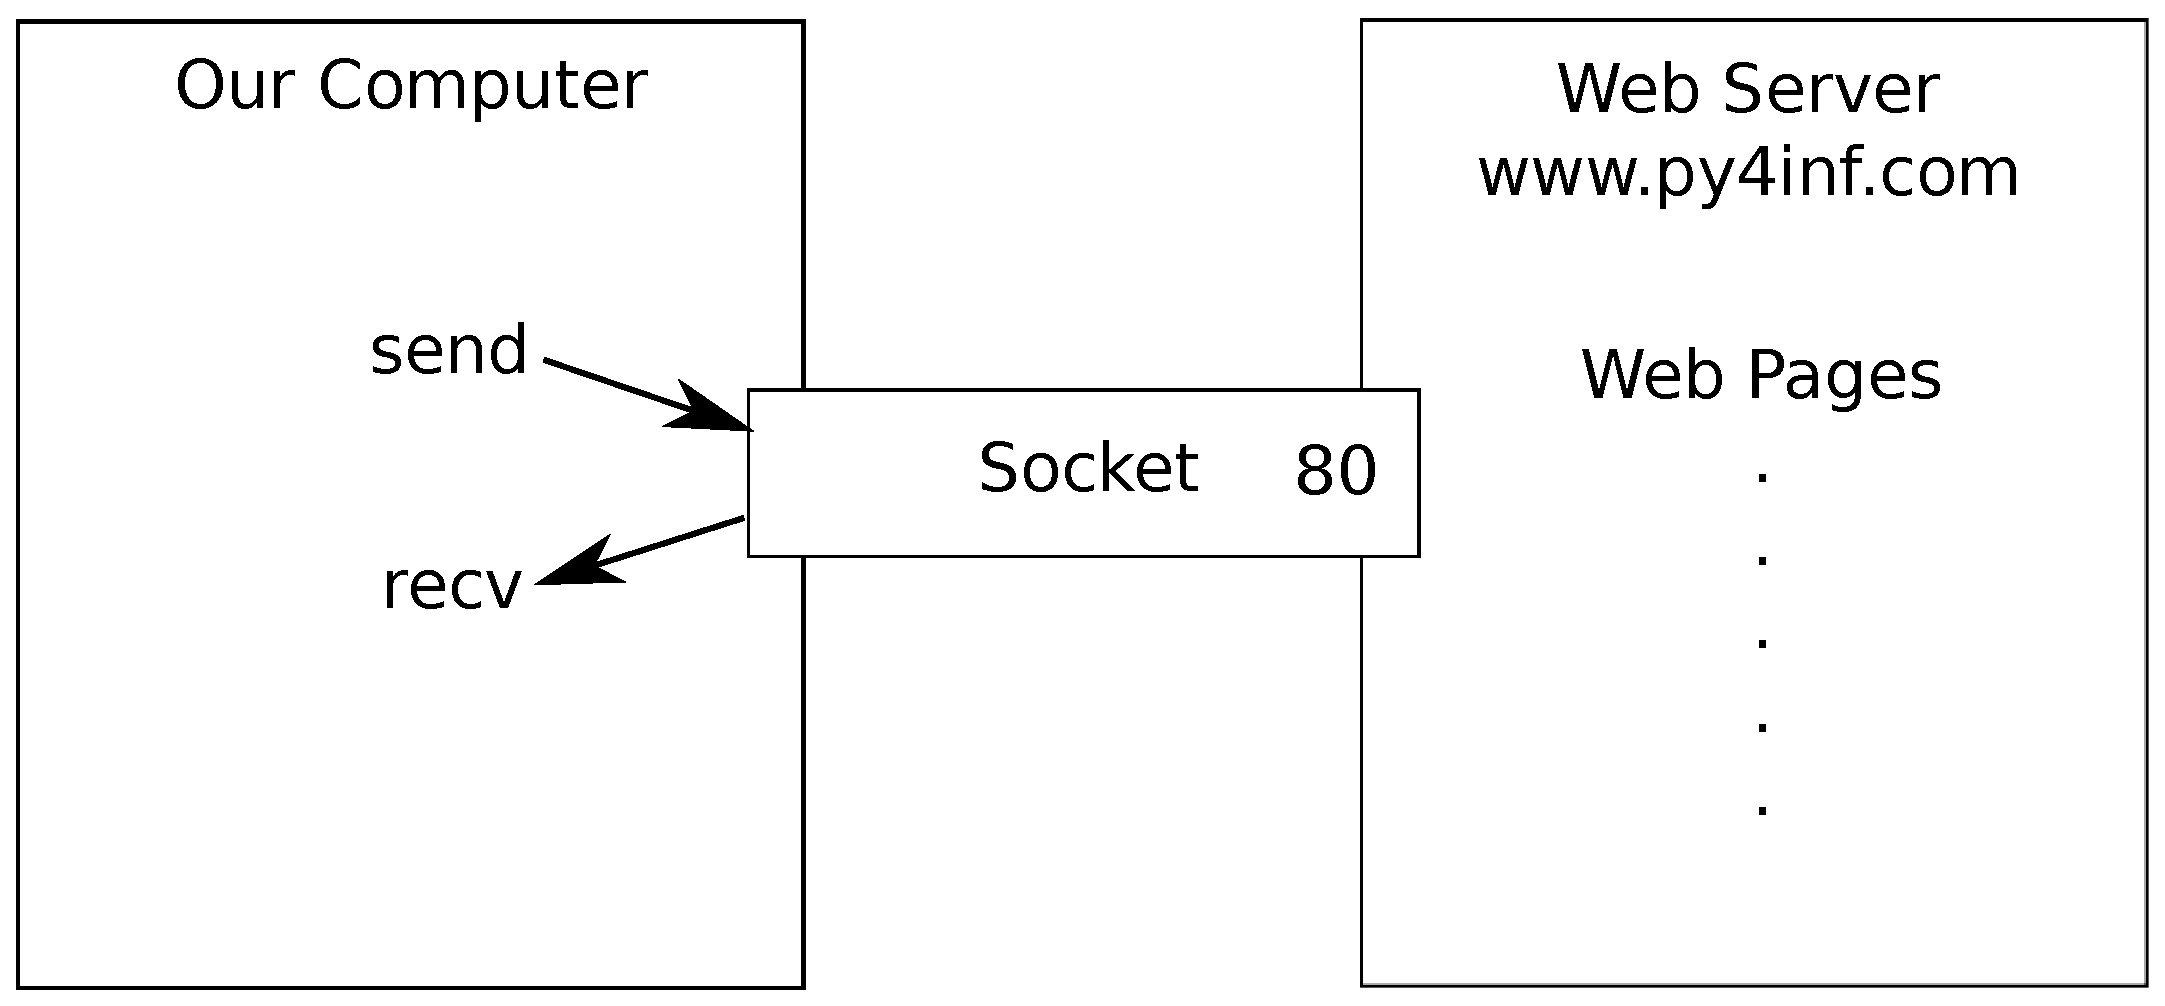
\includegraphics[height=1.50in]{figs2/socket.eps}}
\afterfig

Once we send that blank line, we write a loop that receives data 
in 512 character chunks from the socket and prints the data out 
until there is no more data to read (i.e. the recv() returns 
an empty string).

The program produces the following output:

\beforeverb
\begin{verbatim}
HTTP/1.1 200 OK
Date: Sun, 14 Mar 2010 23:52:41 GMT
Server: Apache
Last-Modified: Tue, 29 Dec 2009 01:31:22 GMT
ETag: "143c1b33-a7-4b395bea"
Accept-Ranges: bytes
Content-Length: 167
Connection: close
Content-Type: text/plain

But soft what light through yonder window breaks
It is the east and Juliet is the sun
Arise fair sun and kill the envious moon
Who is already sick and pale with grief
\end{verbatim}
\afterverb
%
The output starts with headers which the web server sends
to describe the document.
For example, the {\tt Content-Type } header indicated that
the document is a plain text document ({\tt text/plain}).

After the server sends us the headers, it adds a blank line
to indicate the end of the headers and then sends the actual
data of the file {\tt romeo.txt}.

This example shows how to make a low-level network connection
with sockets.   Sockets can be used to communicate with a web
server or with a mail server or many other kinds of servers.
All that is needed is to find the document which describes
the protocol and write the code to send and receive the data
according to the protocol.

However, since the protocol that we use most commonly is
the HTTP (i.e. the web) protocol, Python has a special 
library specifically designed to support the HTTP protocol 
for the retrieval of
documents and data over the web.

\section{Retrieving web pages with {\tt urllib}}

The {\tt urllib} library makes it very easy to retrieve
web pages and process the data in Python.   Using {\tt urllib}
you can treat a web page much like a file.   You simply
indicate which web page you would like to retrieve and
{\tt urllib} handles all of the HTTP protocol details.

The equivalent code to read the {\tt romeo.txt} file
from the web using {\tt urllib} is as follows:

\beforeverb
\begin{verbatim}
import urllib

fhand = urllib.urlopen('http://www.py4inf.com/code/romeo.txt')
for line in fhand:
   print line.strip()
\end{verbatim}
\afterverb
%
Once the web page has been opened with 
{\tt urllib.urlopen} we can treat it like 
a file and read through it using a 
{\tt for} loop.   

When the program runs, we only see the output
of the contents of the file.   The headers
are still sent, but the {\tt urllib} code
consumes the headers and only returns the 
data to us.

\beforeverb
\begin{verbatim}
But soft what light through yonder window breaks
It is the east and Juliet is the sun
Arise fair sun and kill the envious moon
Who is already sick and pale with grief
\end{verbatim}
\afterverb
%

As an example, we can write 
a program to retrieve the data for
{\tt romeo.txt} and compute the frequency
of each word in the file as follows:

\beforeverb
\begin{verbatim}
import urllib

counts = dict()
fhand = urllib.urlopen('http://www.py4inf.com/code/romeo.txt')
for line in fhand:
    words = line.split()
    for word in words:
        counts[word] = counts.get(word,0) + 1   
print counts
\end{verbatim}
\afterverb
%
Again, once we have opened the web page, 
we can read it like a local file.

\section{Parsing HTML and scraping the web}

One of the common uses of the {\tt urllib} capability in Python is 
to {\bf scrape} the web.   Web scraping is when we write a program
that pretends to be a web browser and retrieves pages and then 
examines the data in those pages looking for patterns.

As an example, a search engine such as Google will look at the source 
of one web page and extract the links to other pages and retrieve
those pages, extracting links, and so on.   Using this technique,
Google {\bf spiders} its way through nearly all of the pages on 
the web.   
Google also uses the frequency of links from pages it finds 
to a particular page as one measure of how ``important'' 
a page is and how highly the page should appear in its search results.

There are a number of Python libraries which can help you parse
HTML and extract data from the pages.  Each of the libraries
has its strengths and weaknesses and you can pick one based on 
your needs.

As an example, we will simply parse some HTML input 
and extract links using the {\bf BeautifulSoup} library.   
You can download and install the BeautifulSoup code
from:

\url{www.crummy.com}

You can download and ``install'' BeautifulSoup or you 
can simply place the {\tt BeautifulSoup.py} file in the
same folder as your application.

Even though HTML looks like XML and some pages are carefully 
constructed to be XML, most HTML is generally broken in ways
that cause an XML parser to reject the entire page of HTML as
improperly formed.  BeautifulSoup tolerates highly flawed 
HTML and still lets you easily extract the data you need.

Here is a simple web page:

\beforeverb
\begin{verbatim}
<h1>The First Page</h1>
<p>
If you like, you can switch to the
<a href="http://www.dr-chuck.com/page2.htm">
Second Page</a>.
</p>
\end{verbatim}
\afterverb
%
We will use {\tt urllib} to read the page and then use
{\tt BeautifulSoup} to extract the {\tt href} attributes from the
anchor ({\tt a}) tags.
\index{BeautifulSoup}
\index{HTML}
\index{parsing!HTML}

\beforeverb
\begin{verbatim}
import urllib
from BeautifulSoup import *

url = raw_input('Enter - ')
html = urllib.urlopen(url).read()
soup = BeautifulSoup(html)

# Retrieve all of the anchor tags
tags = soup('a')
for tag in tags:
   print tag.get('href', None)
\end{verbatim}
\afterverb
%
The program prompts for a web address, then opens the web
page, reads the data and passes the data to the BeautifulSoup
parser, and then retrieves all of the anchor tags and prints
out the {\tt href} attribute for each tag.

When the program is run it looks as follows:

\beforeverb
\begin{verbatim}
python urllinks.py 
Enter - http://www.dr-chuck.com/page1.htm
http://www.dr-chuck.com/page2.htm

python urllinks.py 
Enter - http://www.py4inf.com/book.htm
http://www.greenteapress.com/thinkpython/thinkpython.html
http://allendowney.com/
http://www.si502.com/
http://www.lib.umich.edu/espresso-book-machine
http://www.py4inf.com/code
http://www.pythonlearn.com/
\end{verbatim}
\afterverb
%
You can use BeautifulSoup to pull out various parts of each 
tag as follows:
\beforeverb
\begin{verbatim}
import urllib
from BeautifulSoup import *

url = raw_input('Enter - ')
html = urllib.urlopen(url).read()
soup = BeautifulSoup(html)

# Retrieve all of the anchor tags
tags = soup('a')
for tag in tags:
   # Look at the parts of a tag
   print 'TAG:',tag
   print 'URL:',tag.get('href', None)
   print 'Content:',tag.contents[0]
   print 'Attrs:',tag.attrs
\end{verbatim}
\afterverb
%
This produces the following output:
\beforeverb
\begin{verbatim}
python urllink2.py 
Enter - http://www.dr-chuck.com/page1.htm
TAG: <a href="http://www.dr-chuck.com/page2.htm">
Second Page</a>
URL: http://www.dr-chuck.com/page2.htm
Content: [u'\nSecond Page']
Attrs: [(u'href', u'http://www.dr-chuck.com/page2.htm')]
\end{verbatim}
\afterverb
%
These examples only begin to show the power of BeautifulSoup
when it comes to parsing HTML.  See the documentation 
and samples at
\url{www.crummy.com}
for more detail.

\section{Glossary}

\begin{description}

\item[BeautifulSoup:] A Python library for parsing HTML documents
and extracting data from HTML documents
that compensates for most of the imperfections in the HTML that browsers
generally ignore.
You can download the BeautifulSoup code
from 
\url{www.crummy.com}.
\index{BeautifulSoup}

\item[port:] A number that generally indicates which application 
you are contacting when you make a socket connection to a server.
As an example, web traffic usually uses port 80 while e-mail 
traffic uses port 25.
\index{port}

\item[scrape:] When a program pretends to be a web browser and
retrieves a web page and then looks at the web page content. 
Often programs are following the links in one page to find the next
page so they can traverse a network of pages or a social network.
\index{socket}

\item[socket:] A network connection between two applications
where the applications can send and receive data in either direction.
\index{socket}

\item[spider:] The act of a web search engine retrieving a page and
then all the pages linked from a page and so on until they have 
nearly all of the pages on the Internet which they 
use to build their search index.
\index{spider}

\end{description}

\section{Exercises}

\begin{ex}
Change the socket program to prompt the user for the URL so it can read any web page.  
Add error checking using {\tt try} and {\tt except} to handle the condition where the 
user enters an improperly formatted or non-existant URL.  
\end{ex}

\begin{ex}
Change your socket program so that it counts the number of characters it has received 
and stops displaying any text after it has shown 3000 characters.  The program 
should retrieve the entire document and count the total number of characters 
and display the count of the number of characters at the end of the document.
\end{ex}

\begin{ex}
Use {\tt urllib} to replicate the previous exercise of (1) retrieving the document
from a URL, (2) displaying up to 3000 characters, and (3) counting the overall number
of characters in the document.  Don't worry about the headers for this exercise, simply
show the first 3000 characters of the document contents.
\end{ex}

\begin{ex}
Change the {\tt urllinks.py} program to extract paragraph (p) tags
from the retrieved HTML document and simply count how many paragraphs
are in the document and display the count of the paragraphs as the 
output of your program.  Test your program on several small web pages
as well as some larger web pages.
\end{ex}

\begin{ex}
(Advanced) Change the socket program so that it only shows data after the 
headers and a blank line have been received.  Remember that {\tt recv} is
receiving characters (newlines and all) - not lines.
\end{ex}


\chapter{Using Web Services}

Once it became easy to retrieve documents and parse documents 
over HTTP using programs, it did not take long to develop 
an approach where we started producing documents that were specifically
designed to be consumed by other 
programs (i.e. not HTML to be displayed in a browser).

The most common approach when two programs are exchanging data across 
the web is to exchange the data in a format called the ``eXtensible Markup 
Language'' or XML.  

\section{eXtensible Markup Language - XML}

XML looks very similar to HTML, but XML is more structured 
than HTML.  Here is a sample of an XML document:

\beforeverb
\begin{verbatim}
<person>
  <name>Chuck</name>
  <phone type="intl">
     +1 734 303 4456
   </phone>
   <email hide="yes"/>
</person>
\end{verbatim}
\afterverb
%
Often it is helpful to think of an XML document as a tree structure
where there is a top tag {\tt person} and other tags such as {\tt phone}
are drawn as \emph{children} of their parent nodes.

\beforefig
\centerline{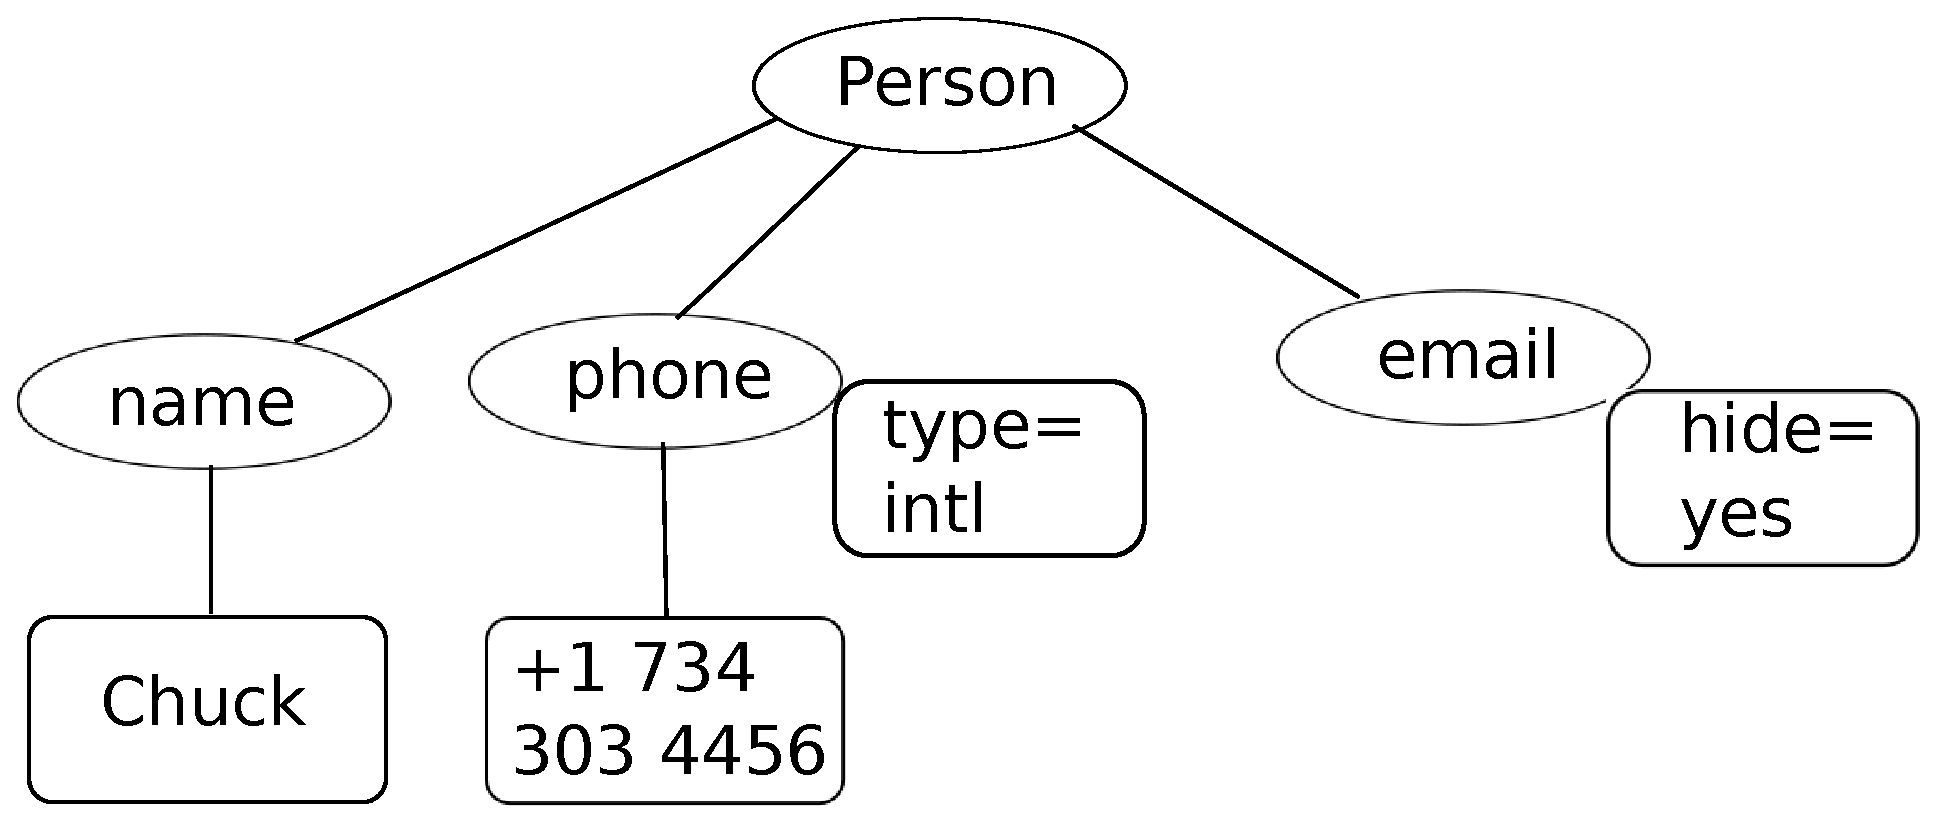
\includegraphics[height=1.50in]{figs2/xml-tree.eps}}
\afterfig

\section{Parsing XML}

Here is a simple application that parses some XML
and extracts some data elements from the XML:

\index{ElementTree}
\index{ElementTree!fromstring}
\index{ElementTree!find}
\beforeverb
\begin{verbatim}
import xml.etree.ElementTree as ET

data = '''
<person>
  <name>Chuck</name>
  <phone type="intl">
     +1 734 303 4456
   </phone>
   <email hide="yes"/>
</person>'''

tree = ET.fromstring(data)
print 'Name:',tree.find('name').text
print 'Attr:',tree.find('email').get('hide')
\end{verbatim}
\afterverb
%
Calling {\tt fromstring} converts the string representation
of the XML into a 'tree' of XML nodes.  When the
XML is in a tree, we have a series of methods which we can call to 
extract portions of data from the XML.  

The {\tt find} function searches through the 
XML tree and retrieves a {\bf node} that matches the specified tag.
Each node can have some text, some attributes (i.e. like hide) and
some ``child'' nodes.   Each node can be the top of a tree of nodes.

\beforeverb
\begin{verbatim}
Name: Chuck
Attr: yes
\end{verbatim}
\afterverb
%
Using an XML parser such as {\tt ElementTree} has the advantage
that while the XML in this example is quite simple, it turns
out that there are many rules regarding valid XML and using 
{\tt ElementTree} allows us to extract data from XML without 
worrying about the rules of XML syntax.

\section{Looping through nodes}

Often the XML has multiple nodes and we need to write a loop
to process all of the nodes.  In the following program, 
we loop through all of the {\tt user} nodes:

\index{ElementTree!findall}
\index{ElementTree!get}
\beforeverb
\begin{verbatim}
import xml.etree.ElementTree as ET

input = '''
<stuff>
    <users>
        <user x="2">
            <id>001</id>
            <name>Chuck</name>
        </user>
        <user x="7">
            <id>009</id>
            <name>Brent</name>
        </user>
    </users>
</stuff>'''

stuff = ET.fromstring(input)
lst = stuff.findall('users/user')
print 'User count:', len(lst)

for item in lst:
    print 'Name', item.find('name').text
    print 'Id', item.find('id').text
    print 'Attribute', item.get('x')
\end{verbatim}
\afterverb
%
The {\tt findall} method retrieves a Python list of sub-trees that
represent the {\tt user} structures in the XML tree.  Then we can 
write a {\tt for} loop that looks at each of the user nodes, and 
prints the {\tt name} and {\tt id} text elements as well as the 
{\tt x} attribute from the {\tt user} node.

\beforeverb
\begin{verbatim}
User count: 2
Name Chuck
Id 001
Attribute 2
Name Brent
Id 009
Attribute 7
\end{verbatim}
\afterverb
%

\section{Application Programming Interfaces (API)}

We now have the ability to exchange data between applications using HyperText
Transport Protocol (HTTP) and a way to represent complex data that we are 
sending back and forth between these applications using eXtensible 
Markup Language (XML).

The next step is to begin to define and document ``contracts'' between 
applications using these techniques. The general name for these 
application-to-application contracts is {\bf Application Program 
Interfaces} or APIs.  When we use an API, generally one program
makes a set of {\bf services} available for use by other applications
and publishes the APIs (i.e. the ``rules'') which must be followed to 
access the services provided by the program.

When we begin to build our programs where the functionality of
our program includes access to services provided by other programs, 
we call the approach a {\bf Service-Oriented Architecture} or SOA.
A SOA approach is one where our overall application makes use of 
the services of other applications.  A non-SOA approach is where the
application is a single stand-alone application which contains all of the
code necessary to implement the application.

We see many examples of SOA when we use the web.  We can go to a single 
web site and book air travel, hotels, and automobiles all from a 
single site.  The data for hotels is not stored on the airline computers. 
Instead, the airline computers contact the services on the hotel computers
and retrieve the hotel data and present it to the user.  When the user
agrees to make a hotel reservation using the airline site, the airline site uses
another web service on the hotel systems to actually make the reservation.
And when it comes to charge your credit card for the whole transaction, 
still other computers become involved in the process.

\beforefig
\centerline{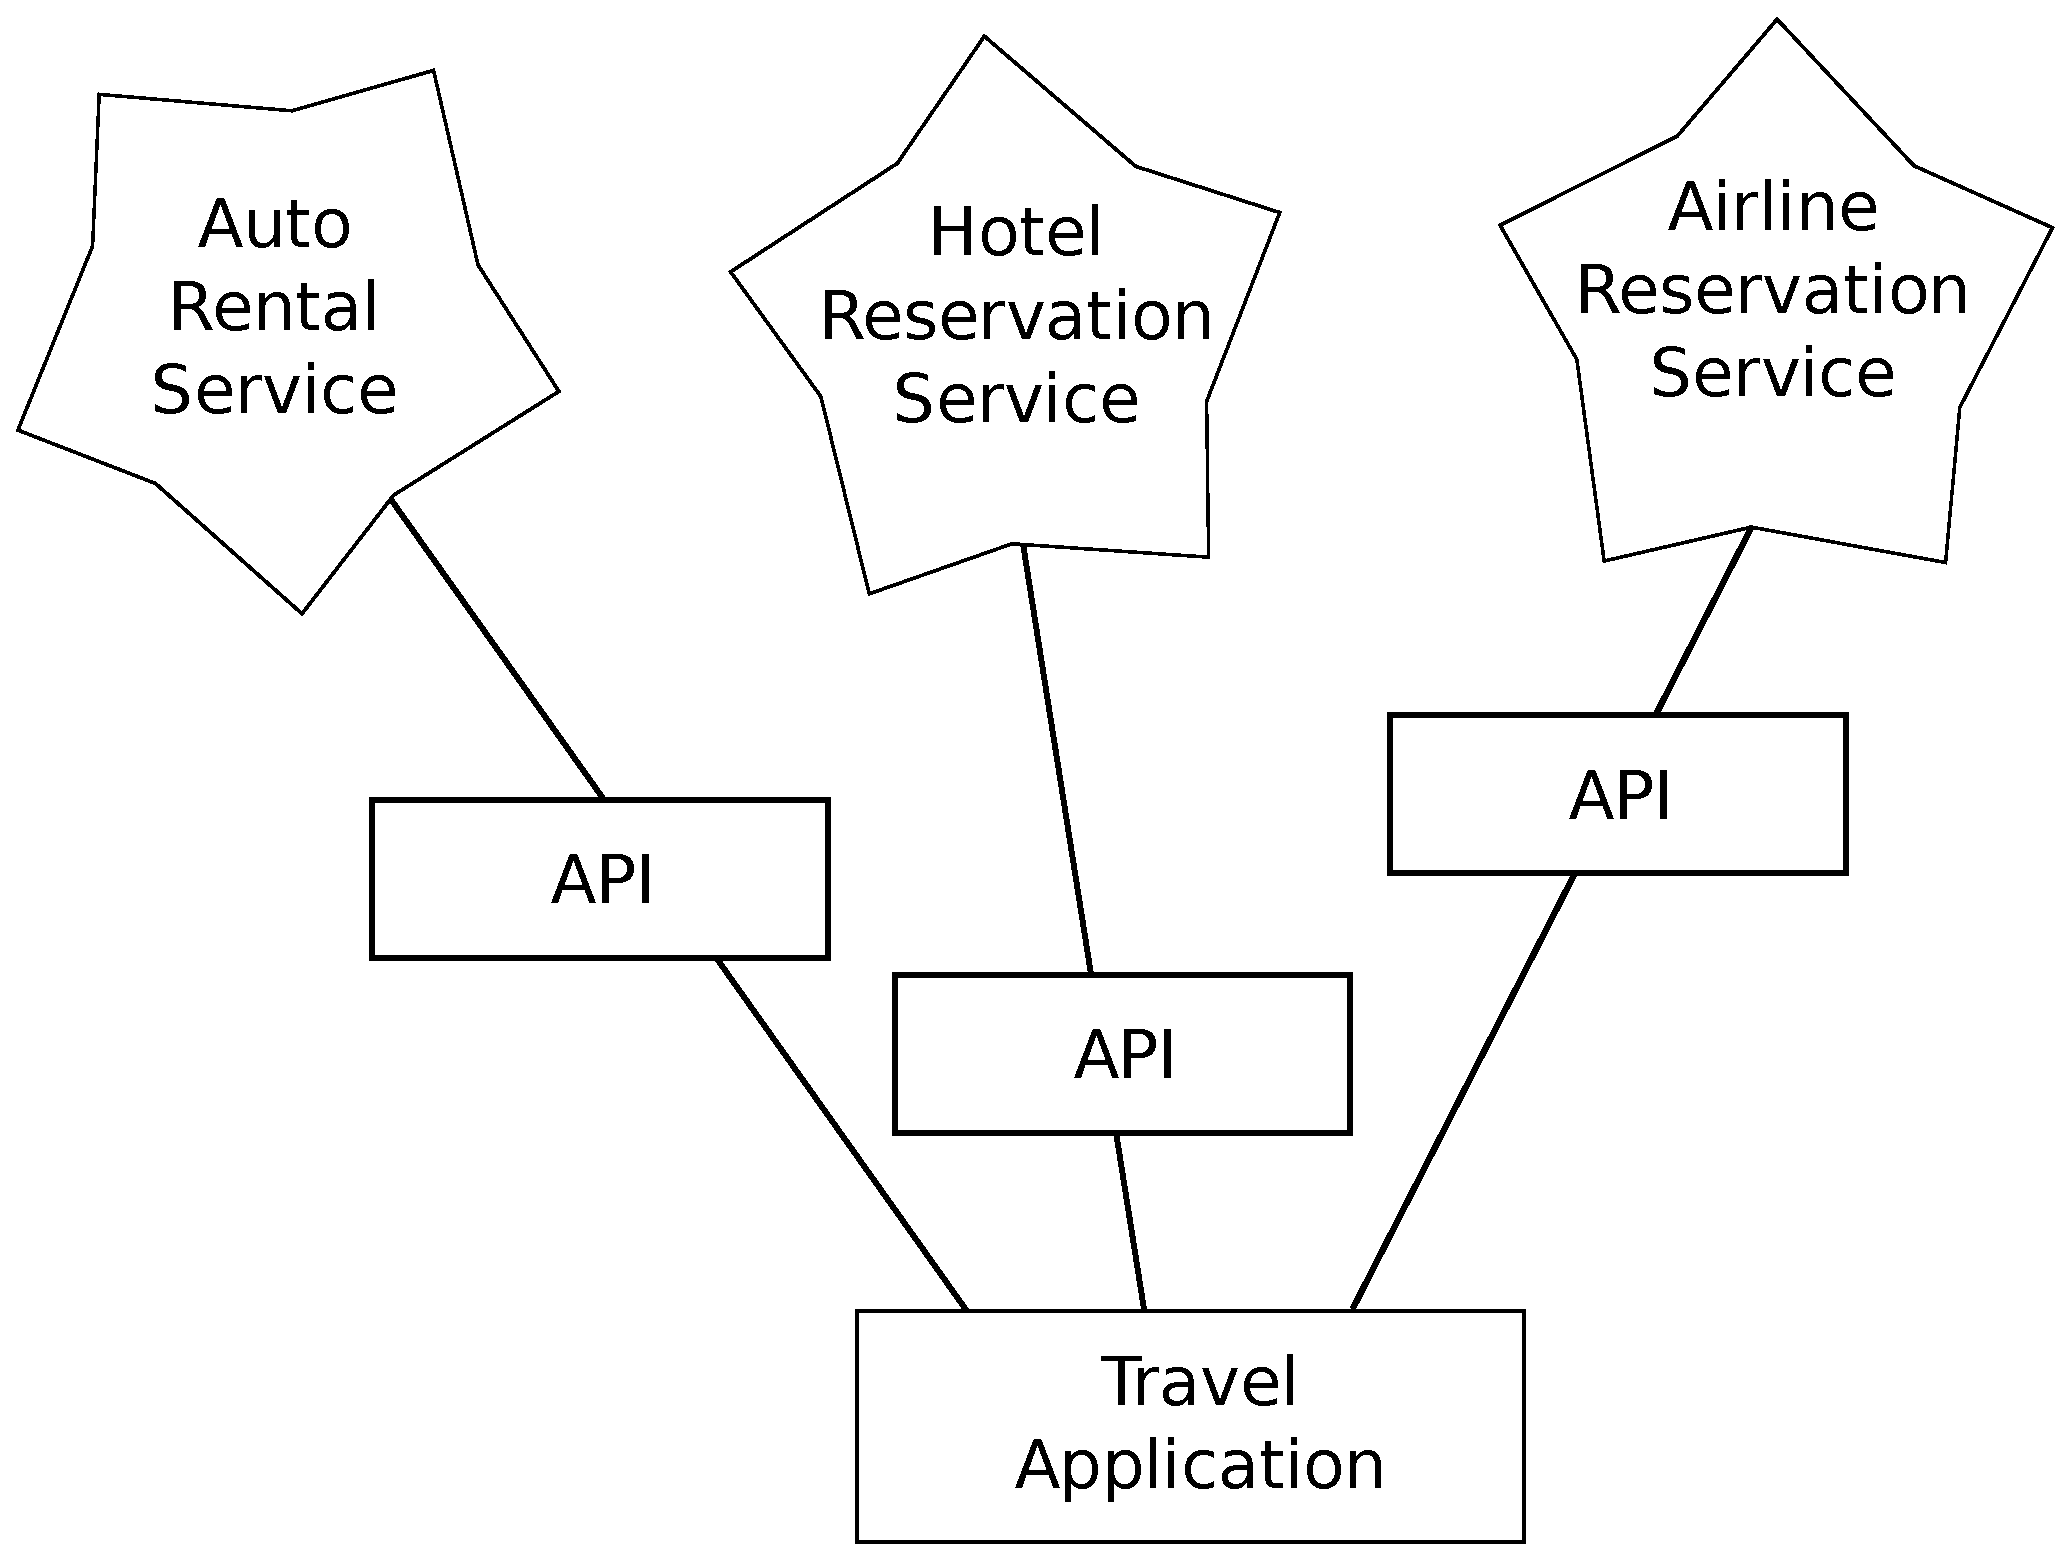
\includegraphics[height=2.50in]{figs2/soa.eps}}
\afterfig

A Service-Oriented Architecture has many advantages including: (1) we 
always maintain only one copy of data - this is particularly important
for things like hotel reservations where we do not want to over-commit
and (2) the owners of the data can set the rules about the use of their 
data.   With these advantages, a SOA system must be carefully designed
to have good performance and meet the user's needs.

When an application makes a set of services in its API available over the web, 
we call these {\bf web services}. 

\section{Twitter web services}

You are probably familiar with the Twitter web site and its
applications \url{http://www.twitter.com}.  Twitter has a very unique
approach to its API/web services in that all of its data is available
to non-Twitter applications using the Twitter API.

Because Twitter has been so liberal in allowing access to its data,
it has enabled thousands of software developers to build their own
customized Twitter-based software.  These additional applications greatly
increase the value of Twitter far beyond simply a web site.  The 
Twitter web services allow the building of whole new applications that
the Twitter team may never have thought of.  It is said that over 90 percent
of the use of Twitter is through the API (i.e. not through the {\tt twitter.com}
web user interface).

You can view the Twitter API documentation at 
\url{http://apiwiki.twitter.com/}.  The Twitter API is an example
of the REST style of web services.
We will focus on the Twitter API
to retrieve a list of a user's friends and their statuses.  As an 
example, you can visit the following URL:

\url{http://api.twitter.com/1/statuses/friends/drchuck.xml}

To see a list of the friends of the twitter account {\tt drchuck}.
It may look like a mess in your browser.   To see the actual XML
returned by Twitter, you can view the source of the returned
``web page''.

We can retrieve this same XML using Python using the {\tt urllib}
utility:

\beforeverb
\begin{verbatim}
import urllib

TWITTER_URL = 'http://api.twitter.com/l/statuses/friends/ACCT.xml'

while True:
    print ''
    acct = raw_input('Enter Twitter Account:')
    if ( len(acct) < 1 ) : break
    url = TWITTER_URL.replace('ACCT', acct)
    print 'Retrieving', url
    document = urllib.urlopen (url).read()
    print document[:250]
\end{verbatim}
\afterverb
%
The program prompts for a Twitter account and opens the URL
for the friends and statuses API and then retrieves the 
text from the URL and shows us the first 250 characters of
the text.

\beforeverb
\begin{verbatim}
python twitter1.py

Enter Twitter Account:drchuck
Retrieving http://api.twitter.com/l/statuses/friends/drchuck.xml
<?xml version="1.0" encoding="UTF-8"?>
<users type="array">
<user>
  <id>115636613</id>
  <name>Steve Coppin</name>
  <screen_name>steve_coppin</screen_name>
  <location>Kent, UK</location>
  <description>Software developing, best practicing, agile e

Enter Twitter Account:
\end{verbatim}
\afterverb
%
In this application, we have retrieved the XML exactly as if it were
an HTML web page.  If we wanted to extract data from the XML, we 
could use Python string functions but this would become pretty complex
as we tried to really start to dig into the XML in detail.

If we were to dump out some of the retrieved XML it would look roughly as follows:

\beforeverb
\begin{verbatim}
<?xml version="1.0" encoding="UTF-8"?>
<users type="array">
  <user>
    <id>115636613</id>
    <name>Steve Coppin</name>
    <screen_name>steve_coppin</screen_name>
    <location>Kent, UK</location>
    <status>
      <id>10174607039</id>
      <source>web</source>
      </status>
  </user>
  <user>
    <id>17428929</id>
    <name>davidkocher</name>
    <screen_name>davidkocher</screen_name>
    <location>Bern</location>
    <status>
      <id>10306231257</id>
      <text>@MikeGrace If possible please post a detailed bug report </text>
    </status>
  </user>
  ...
\end{verbatim}
\afterverb
%
The top level tag is a {\tt users} and there are multiple {\tt user} tags
below within the {\tt users} tag.   There is also a {\tt status} tag below
the {\tt user} tag.  

\section{Handling XML data from an API}

When we receive well-formed XML data from an API, we generally use
an XML parser such as {\tt ElementTree} to extract information from
the XML data.

In the program below, we retrieve the friends and statuses from
the Twitter API and then parse the returned XML to show the first
four friends and their statuses.

\beforeverb
\begin{verbatim}
import urllib
import xml.etree.ElementTree as ET

TWITTER_URL = 'http://api.twitter.com/l/statuses/friends/ACCT.xml'

while True:
    print ''
    acct = raw_input('Enter Twitter Account:')
    if ( len(acct) < 1 ) : break
    url = TWITTER_URL.replace('ACCT', acct)
    print 'Retrieving', url
    document = urllib.urlopen (url).read()
    print 'Retrieved', len(document), 'characters.' 
    tree = ET.fromstring(document)
    count = 0
    for user in tree.findall('user'):
        count = count + 1
        if count > 4 : break
        print user.find('screen_name').text
        status =  user.find('status')
        if status : 
            txt = status.find('text').text
            print '  ',txt[:50]
\end{verbatim}
\afterverb
%
We use the {\tt findall} method to get a list of the {\tt user} 
nodes and loop through the list using a {\tt for } loop.  
For each {\tt user} node, we pull out the text of the \verb"screen_name" node
and then pull out the {\tt status} node.   If there is a {\tt status}
node, we pull out the text of the {\tt text} node and print the first 50 
characters of the status text.

The pattern is pretty straightforward, we use {\tt findall} and {\tt find}
to pull out a list of nodes or a single node and then if a node is a complex
element with more sub-nodes we look deeper into the node until we reach the 
text element that we are interested in.

The program runs as follows:

\beforeverb
\begin{verbatim}
python twitter2.py 

Enter Twitter Account:drchuck
Retrieving http://api.twitter.com/l/statuses/friends/drchuck.xml
Retrieved 193310 characters.
steve_coppin
   Looking forward to some "oh no the markets closed,
davidkocher
   @MikeGrace If possible please post a detailed bug 
hrheingold
   From today's Columbia Journalism Review, on crap d
huge_idea
   @drchuck  #cnx2010 misses you, too.  Thanks for co

Enter Twitter Account:hrheingold
Retrieving http://api.twitter.com/l/statuses/friends/hrheingold.xml
Retrieved 208081 characters.
carr2n
   RT @tysone: Saturday's proclaimation by @carr2n pr
tiffanyshlain
   RT @ScottKirsner: Turning smartphones into a tool 
soniasimone
   @ACCompanyC Funny, smart, cute, and also nice! He 
JenStone7617
   Watching "Changing The Equation: High Tech Answers

Enter Twitter Account:
\end{verbatim}
\afterverb
%
While the code for parsing the XML and extracting the fields
using {\tt ElementTree} takes a few lines to express what 
we are looking for in the XML, it is much simpler than trying 
to use Python string parsing to pull apart the XML and find 
the data elements.

\section{Glossary}

\begin{description}

\item[API:] Application Program Interface - A contract between
applications that defines the patterns of interaction between 
two application components.
\index{API}

\item[ElementTree:] A built-in Python library used to parse XML data.
\index{ElementTree}

\item[XML:] eXtensible Markup Language - A format that allows for 
the markup of structured data.
\index{XML}
\index{eXtensible Markup Language}

\item[REST:] REpresentational State Transfer - A style of Web Services 
that provide access to resources within an application using the HTTP
protocol.
\index{ElementTree}

\item[SOA:] Service Oriented Architecture - when an application is 
made of components connected across a network.
\index{SOA}
\index{Service Oriented Architecture}

\end{description}

\section{Exercises}

\begin{ex}
Change the program that retrieves twitter data to also
print out the location for each of the friends
indented under the name by two spaces as follows:

\beforeverb
\begin{verbatim}
Enter Twitter Account:drchuck
Retrieving http://api.twitter.com/l/statuses/friends/drchuck.xml
Retrieved 194533 characters.
steve_coppin
   Kent, UK
   Looking forward to some "oh no the markets closed,
davidkocher
   Bern
   @MikeGrace If possible please post a detailed bug 
hrheingold
   San Francisco Bay Area
   RT @barrywellman: Lovely AmBerhSci Internet & Comm
huge_idea
   Boston, MA
   @drchuck  #cnx2010 misses you, too.  Thanks for co
\end{verbatim}
\afterverb
%
\end{ex}

\chapter{Using databases and Structured Query Language (SQL)}

\section{What is a database?}
\index{database}

A {\bf database} is a file that is organized for storing data.
Most databases are organized like a dictionary in the sense
that they map from keys to values.  The biggest difference
is that the database is on disk (or other permanent storage),
so it persists after the program ends.  Because a database is
stored on permanent storage, it can store far more data than
a dictionary, which is limited to the size of the memory 
in the computer.

\index{database!indexes}
Like a dictionary, database software is designed to keep 
the inserting and accessing of data very fast, even for large
amounts of data.   Database software maintains its performance by 
building {\bf indexes} as data is added to the database
to allow the computer to jump quickly to a particular
entry.

There are many different database systems which are used for a wide
variety of purposes including: Oracle, MySQL, Microsoft SQL Server, 
PostgreSQL, and SQLite.  We focus on SQLite in this book because
it is a very common database and is already built into Python.  
SQLite is designed to be \emph{embedded} into other applications
to provide database support within the application.  For example,
the Firefox browser also uses the SQLite database internally as do 
many other products.

\url{http://sqlite.org/}

SQLite is well suited to some of the data manipulation problems that we 
see in Informatics such as the Twitter spidering application that we 
describe in this chapter.

\section{Database concepts}

When you first look at a database it looks like a 
spreadsheet with multiple sheets.   The primary data structures 
in a database are:
{\bf tables}, {\bf rows}, and {\bf columns}.  

\beforefig
\centerline{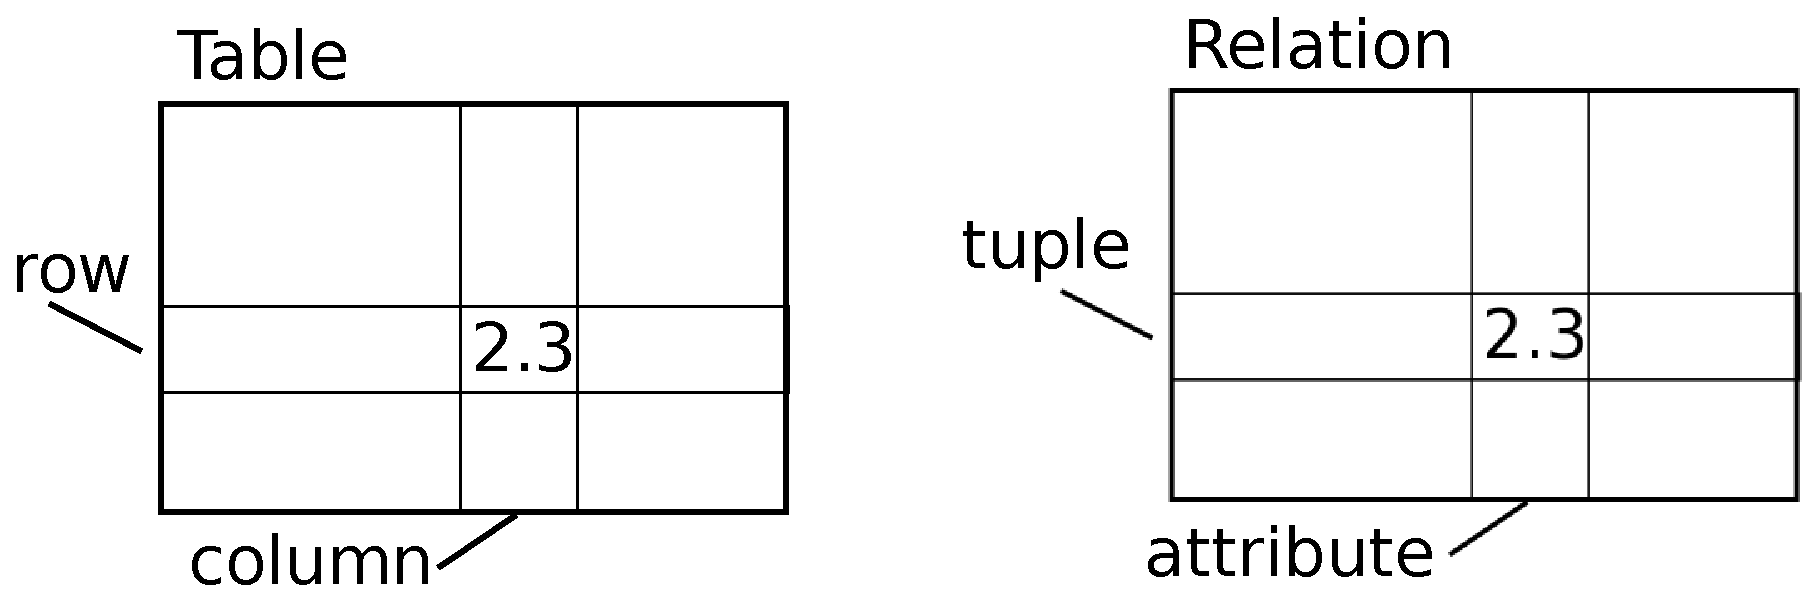
\includegraphics[height=1.50in]{figs2/relational.eps}}
\afterfig

In technical descriptions of relational databases the concepts of 
table, row, and column are more formally referred
to as {\bf relation}, {\bf tuple}, and {\bf attribute}, respectively.
We will use the less formal terms in this chapter.

\section{SQLite Database Browser}

While this chapter will focus on using Python to work with data 
in SQLite database files, many operations can be done more
conveniently using a desktop program called the {\bf SQLite
Database Browser} which is freely available from:

\url{http://sourceforge.net/projects/sqlitebrowser/}

Using the browser you can easily create tables, insert data, edit data, 
or run simple SQL queries on the data in the database.

\beforefig
\centerline{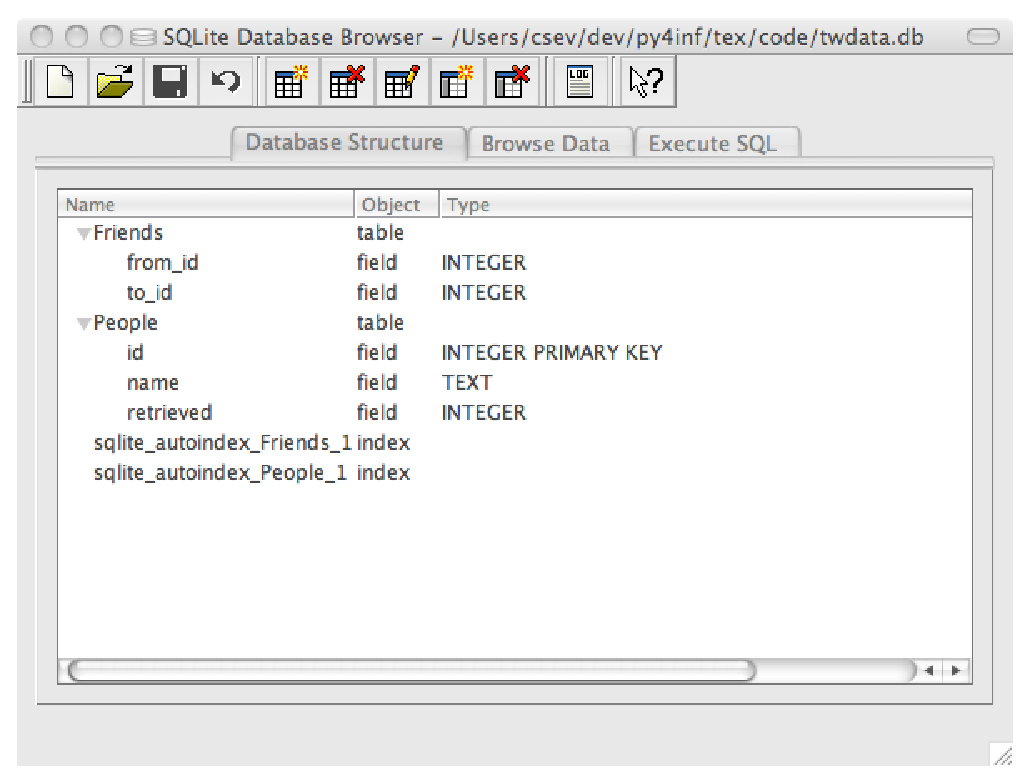
\includegraphics[height=3.00in]{figs2/sqlite.eps}}
\afterfig

In a sense, the database browser is similar to a text editor
when working with text files.   When you want to do one or
very few operations on a text file, you can just open it
in a text editor and make the changes you want.   When you have 
many changes that you need to do to a text file, often you 
will write a simple Python program.  You will find the same 
pattern when working with databases.  You will do simple
operations in the database browser and more complex operations
will be most conveniently done in Python.

\section{Creating a database table}

Databases require more defined structure than Python lists 
or dictionaries\footnote{SQLite actually does allow some 
flexibility in the type of data stored in a column,
but we will keep our data types strict in this chapter
so the concepts apply equally to other database systems 
such as MySQL.}.  

When we create a database {\bf table} we
must tell the database in advance the names of each of the
{\bf columns} in the table and the type of data which we are 
planning to store in each {\bf column}.   When the database software
knows the type of data in each column, it can choose the most 
efficient way to store and lookup the data based on the type of
data. 

You can look at the various data types supported by SQLite
at the following url:

\url{http://www.sqlite.org/datatypes.html}

Defining structure for your data up front may seem inconvenient
at the beginning, but the payoff is fast access to your data 
even when the database contains a large amount of data.

The code to create a database file and a table 
named {\tt Tracks} with two columns in the 
database is as follows:

\index{sqlite3 module}
\index{module!sqlite3}
\beforeverb
\begin{verbatim}
import sqlite3

conn = sqlite3.connect('music.db')
cur = conn.cursor()

cur.execute('DROP TABLE IF EXISTS Tracks ')
cur.execute('CREATE TABLE Tracks (title TEXT, plays INTEGER)')

conn.close()
\end{verbatim}
\afterverb
%
\index{connect function}
\index{function!connect}
\index{cursor function}
\index{function!cursor}
The {\tt connect} operation makes a ``connection'' to the database 
stored in the file {\tt music.db} in the current directory.   If
the file does not exist, it will be created.  The reason this
is called a ``connection'' is that sometimes the database is stored
on a separate ``database server'' from the server on which we 
are running our application.  In our simple examples 
the database will just be a local file in the same directory
as the Python code we are running.

A {\bf cursor} is like a file handle that we can use to perform
operations on the data stored in the database.  Calling 
{\tt cursor()} is very similar conceptually to calling
{\tt open()} when dealing with text files.

\beforefig
\centerline{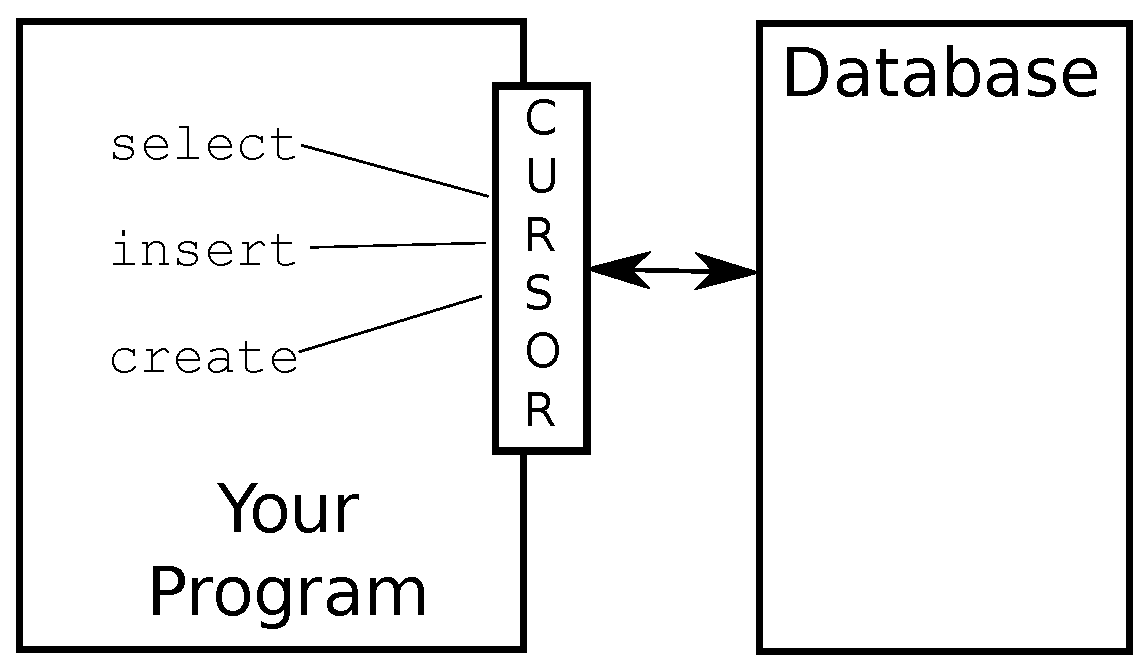
\includegraphics[height=1.50in]{figs2/cursor.eps}}
\afterfig

Once we have the cursor, we can begin to execute 
commands on the contents of the database using the {\tt execute()}
method.

Database commands are expressed in a special language that has 
been standardized across many different database vendors 
to allow us to learn a single database language.   The database
language is called {\bf Structured Query Language} or {\bf SQL}
for short.

\url{http://en.wikipedia.org/wiki/SQL}

In our example, we are executing two SQL commands in our database.
As a convention, we will show the SQL keywords in uppercase 
and the parts of the command that we are adding (such as the
table and column names) will be shown in lowercase.

The first SQL command removes the {\tt Tracks} table from the 
database if it exists.  This pattern is simply to allow us to 
run the same program to create the {\tt Tracks} table over 
and over again without causing an error.  Note that the
{\tt DROP TABLE} command deletes the table and all of its contents
from the database (i.e. there is no ``undo'').

\beforeverb
\begin{verbatim}
cur.execute('DROP TABLE IF EXISTS Tracks ')
\end{verbatim}
\afterverb
%
The second command creates a table named
{\tt Tracks} with a text column named {\tt title}
and an integer column named {\tt plays}.

\beforeverb
\begin{verbatim}
cur.execute('CREATE TABLE Tracks (title TEXT, plays INTEGER)')
\end{verbatim}
\afterverb
%
Now that we have created a table named {\tt Tracks}, we can put some data
into that table using the SQL {\tt INSERT} operation.   Again, we begin
by making a connection to the database and obtaining the {\tt cursor}.
We can then execute SQL commands using the cursor.

The SQL {\tt INSERT} command indicates which table we are using 
and then defines a new row by listing the fields we want to 
include {\tt (title, plays) } followed by the {\tt VALUES} we want
placed in the new row in the table.   We specify the values
as question marks {\tt (?, ?)} to indicate that the actual 
values are passed in as a tuple {\tt ( 'My Way', 15 ) } as the
second parameter to the {\tt execute()} call.

\beforeverb
\begin{verbatim}
import sqlite3

conn = sqlite3.connect('music.db')
cur = conn.cursor()

cur.execute('INSERT INTO Tracks (title, plays) VALUES ( ?, ? )', 
    ( 'Thunderstruck', 20 ) )
cur.execute('INSERT INTO Tracks (title, plays) VALUES ( ?, ? )', 
    ( 'My Way', 15 ) )
conn.commit()

print 'Tracks:'
cur.execute('SELECT title, plays FROM Tracks')
for row in cur :
   print row

cur.execute('DELETE FROM Tracks WHERE plays < 100')
conn.commit()

cur.close()
\end{verbatim}
\afterverb
%
First we {\tt INSERT} two rows into our table and use {\tt commit()} 
to force the data to be written to the database file.

\beforefig
\centerline{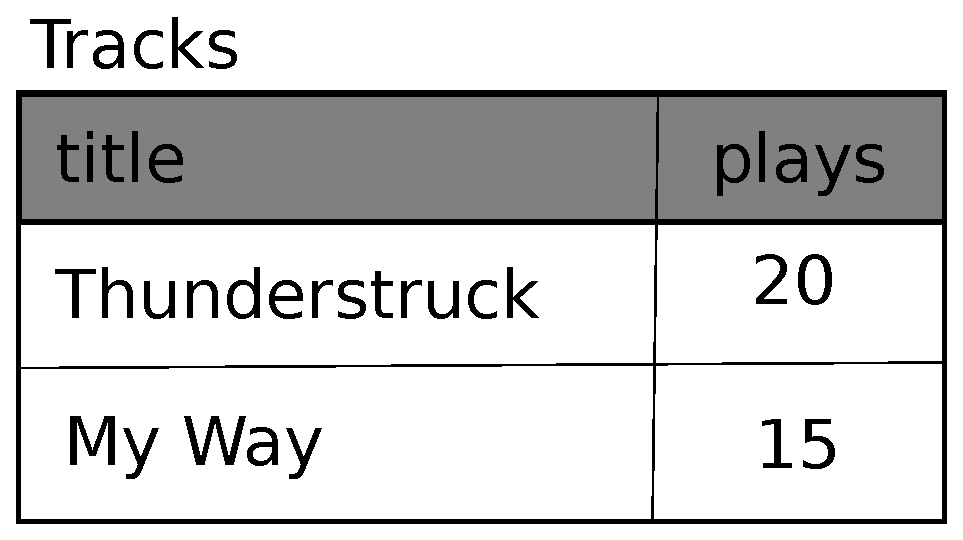
\includegraphics[height=1.00in]{figs2/tracks.eps}}
\afterfig

Then we use the {\tt SELECT} command
to retrieve the rows we just inserted from the table.  
On the 
{\tt SELECT} command, we indicate which columns we would like {\tt (title, plays)}
and indicate which table we want to retrieve the data from.  After we 
execute the {\tt SELECT} statement, the cursor is something we can loop through
in a {\tt for} statement.   For efficiency,
the cursor does not read all of the data from the
database when we execute the {\tt SELECT} statement.  
Instead, the data is read on-demand
as we loop through the rows in the {\tt for} statement.

The output of the program is as follows:

\beforeverb
\begin{verbatim}
Tracks:
(u'Thunderstruck', 20)
(u'My Way', 15)
\end{verbatim}
\afterverb
%
\index{Unicode}
Our {\tt for} loop finds two rows, and each row is a Python tuple with the
first value as the {\tt title} and the second value as the number of {\tt plays}.
Do not be concerned that the title strings are shown starting with 
{\tt u'}.  This is an indication that the strings are {\bf Unicode} strings
that are capable of storing non-Latin character sets.

At the very end of the program, we execute an SQL command to {\tt DELETE} 
the rows we have just created so we can run the program over and over.
The {\tt DELETE} command shows the use of a {\tt WHERE} clause that
allows us to express a selection criterion so that we can ask the database
to apply the command to only the rows that match the criterion.  In this example
the criterion happens to apply to all the rows so we empty the table
out so we can run the program repeatedly.  After the {\tt DELETE} is performed
we also call {\tt commit()} to force the data to be removed from the database.

\section{Structured Query Language (SQL) summary}

So far, we have been using the Structured Query Language in our Python
examples and have covered many of the basics of the SQL commands.
In this section, we look at the SQL language in particular
and give an overview of SQL syntax.

Since there are so many different database vendors, the Structured Query
Language (SQL) was standardized so we could communicate in a portable
manner to database systems from multiple vendors.

A relational database is made up of tables, rows, and columns.  The columns
generally have a type such as text, numeric, or date data.  When we create
a table, we indicate the names and types of the columns:

\beforeverb
\begin{verbatim}
CREATE TABLE Tracks (title TEXT, plays INTEGER)
\end{verbatim}
\afterverb
%
To insert a row into a table, we use the SQL {\tt INSERT} command:

\beforeverb
\begin{verbatim}
INSERT INTO Tracks (title, plays) VALUES ('My Way', 15)
\end{verbatim}
\afterverb
%
The {\tt INSERT} statement specifies the table name, and then a list of
the fields/columns that you would like to set in the new row, and then 
the keyword {\tt VALUES} and then a list of corresponding values 
for each of the fields.

The SQL {\tt SELECT} command is used to retrieve rows and columns from a database.
The {\tt SELECT} statement lets you specify which columns you would
like to retrieve as well as a {\tt WHERE} clause to select which 
rows you would like to see.  It also allows an optional 
{\tt ORDER BY} clause to control the sorting of the returned rows.

\beforeverb
\begin{verbatim}
SELECT * FROM Tracks WHERE title = 'My Way'
\end{verbatim}
\afterverb
%
Using \verb"*" indicates that you want the database to return all of 
the columns for each row that matches the {\tt WHERE} clause.  

Note, unlike in Python, in a SQL {\tt WHERE} clause 
we use a single equal sign 
to indicate a test for equality rather than a double equal sign.
Other logical operations allowed in a {\tt WHERE} clause include 
\verb"<",
\verb">",
\verb"<=",
\verb">=",
\verb"!=",
as well as {\tt AND} and {\tt OR} and parentheses
to build your logical expressions.

You can request that the returned rows be sorted by one of 
the fields as follows:

\beforeverb
\begin{verbatim}
SELECT title,plays FROM Tracks ORDER BY title
\end{verbatim}
\afterverb
%
To remove a row, you need a {\tt WHERE} clause on an SQL {\tt DELETE}
statement.  The {\tt WHERE} clause determines which rows are to be deleted:

\beforeverb
\begin{verbatim}
DELETE FROM Tracks WHERE title = 'My Way'
\end{verbatim}
\afterverb
%
It is possible to {\tt UPDATE} a column or columns within one or more rows
in a table using the SQL {\tt UPDATE} statement as follows:

\beforeverb
\begin{verbatim}
UPDATE Tracks SET plays = 16 WHERE title = 'My Way'
\end{verbatim}
\afterverb
%
The {\tt UPDATE} statement specifies a table and 
then a list of fields and values to change after the {\tt SET} 
keyword and then an optional {\tt WHERE} clause to select
the rows that are to be updated.  A single {\tt UPDATE} statement
will change all of the rows that match the {\tt WHERE} clause, or if 
a {\tt WHERE} clause is not specified, it performs the {\tt UPDATE}
on all of the rows in the table.

These four basic SQL commands (INSERT, SELECT, UPDATE, and DELETE) allow 
the four basic operations needed to create and maintain data.


\section{Spidering Twitter using a database}

In this section, we will create a simple spidering program that will 
go through Twitter accounts and build a database of them.
\emph{Note: Be very careful when running this program.  You do not
want to pull too much data or run the program for too long and
end up having your Twitter access shut off.}

One of the problems of any kind of spidering program is that it 
needs to be able to be stopped and restarted many times and 
you do not want to lose the data that you have retrieved so far.
You don't want to always restart your data retrieval at the
very beginning so we want to store data as we retrieve it so our
program can start back up and pick up where it left off.

We will start by retrieving one person's Twitter friends and their
statuses, looping through the list of friends, and adding each 
of the friends to a database to be retrieved in the future.  After
we process one person's Twitter friends, we check in our database
and retrieve one of the friends of the friend.  We do this over and
over, picking an ``unvisited'' person, retrieving their friend list
and adding friends we have not seen to our list for a future visit.

We also track how many times we have seen a particular friend in the
database to get some sense of ``popularity''.

By storing our list of known accounts and whether 
we have retrieved the account or not, 
and how popular the account is in a database on the disk
of the computer, we can stop and
restart our program as many times as we like.

% TODO: Add a reference to the right spot
This program is a bit complex. It is based on the code 
from the exercise earlier in the book that uses
the Twitter API.

Here is the source code for our Twitter spidering application:

\beforeverb
\begin{verbatim}
import sqlite3
import urllib
import xml.etree.ElementTree as ET

TWITTER_URL = 'http://api.twitter.com/l/statuses/friends/ACCT.xml'

conn = sqlite3.connect('twdata.db')
cur = conn.cursor()

cur.execute('''
CREATE TABLE IF NOT EXISTS 
Twitter (name TEXT, retrieved INTEGER, friends INTEGER)''')

while True:
    acct = raw_input('Enter a Twitter account, or quit: ')
    if ( acct == 'quit' ) : break
    if ( len(acct) < 1 ) :
        cur.execute('SELECT name FROM Twitter WHERE retrieved = 0 LIMIT 1')
        try:
            acct = cur.fetchone()[0]
        except:
            print 'No unretrieved Twitter accounts found'
            continue

    url = TWITTER_URL.replace('ACCT', acct)
    print 'Retrieving', url
    document = urllib.urlopen (url).read()
    tree = ET.fromstring(document)

    cur.execute('UPDATE Twitter SET retrieved=1 WHERE name = ?', (acct, ) )

    countnew = 0
    countold = 0
    for user in tree.findall('user'):
        friend = user.find('screen_name').text
        cur.execute('SELECT friends FROM Twitter WHERE name = ? LIMIT 1', 
            (friend, ) )
        try:
            count = cur.fetchone()[0]
            cur.execute('UPDATE Twitter SET friends = ? WHERE name = ?', 
                (count+1, friend) )
            countold = countold + 1
        except:
            cur.execute('''INSERT INTO Twitter (name, retrieved, friends) 
                VALUES ( ?, 0, 1 )''', ( friend, ) )
            countnew = countnew + 1
    print 'New accounts=',countnew,' revisited=',countold
    conn.commit()

cur.close()
\end{verbatim}
\afterverb
%
Our database is stored in the file {\tt twdata.db} and it has one 
table named {\tt Twitter} and each row in the {\tt Twitter} table
has a column for the account name, whether we have retrieved the friends
of this account, and how many times this account has been ``friended''.

In the main loop of the program, we prompt the user for a Twitter
account name or ``quit'' to exit the program.  
If the user enters a Twitter account, we retrieve the 
list of friends and statuses
for that user and add each friend to the database if 
not already in the database.  If the friend is already in the list, 
we add one to the {\tt friends} field in the row in the database.

If the user presses enter, we look in the database for the next 
Twitter account that we have not yet retrieved and retrieve the
friends and statuses for that account, add them to the database 
or update them and increase their {\tt friends count}.

Once we retrieve the list of friends and statuses, we loop 
through all of the {\tt user} items in the returned XML
and retrieve the \verb"screen_name" for each user.  Then we use
the {\tt SELECT } statement to see if we already have stored this
particular \verb"screen_name" in the database and retrieve the
friend count ({\tt friends}) if the record exists.

\beforeverb
\begin{verbatim}
    countnew = 0
    countold = 0
    for user in tree.findall('user'):
        friend = user.find('screen_name').text
        cur.execute('SELECT friends FROM Twitter WHERE name = ? LIMIT 1', 
            (friend, ) )
        try:
            count = cur.fetchone()[0]
            cur.execute('UPDATE Twitter SET .riends = ? WHERE name = ?', 
                (count+1, friend) )
            countold = countold + 1
        except:
            cur.execute('''INSERT INTO Twitter (name, retrieved, friends) 
                VALUES ( ?, 0, 1 )''', ( friend, ) )
            countnew = countnew + 1
    print 'New accounts=',countnew,' revisited=',countold
    conn.commit()
\end{verbatim}
\afterverb
%
Once the cursor executes the {\tt SELECT} statement, 
we must retrieve the rows.  We could do this with a {\tt for} 
statement, but since we are only retrieving
one row ({\tt LIMIT 1}), we can use the {\tt fetchone()} method to fetch the
first (and only) row that is the result of the {\tt SELECT} operation.  
Since {\tt fetchone()} returns the row as a {\bf tuple} (even though there is only
one field), we take the first value from the tuple using {\tt [0]} to get the 
current friend count into the variable {\tt count}.  

If this retrieval is successful, we use the SQL {\tt UPDATE} statement with a 
{\tt WHERE} clause to add one to the {\tt friends} column for the row that 
matches the friend's account.  Notice that there are two placeholders (i.e.
question marks) in the SQL, and the second parameter to the {\tt execute()} is
a two-element tuple which holds the values to be substituted into the SQL
in place of the question marks.

If the code in the {\tt try} block fails it is probably because no record
matched the {\tt WHERE name = ?} clause on the SELECT statement.  So in the
{\tt except} block, we use the SQL {\tt INSERT} statement to add the friend's
\verb"screen_name" to the table with an indication that we have not yet 
retrieved the \verb"screen_name" and setting the friend count to zero.

So the first time the program runs and we enter a Twitter account, the program
runs as follows:
\beforeverb
\begin{verbatim}
Enter a Twitter account, or quit: drchuck
Retrieving http://api.twitter.com/l/statuses/friends/drchuck.xml
New accounts= 100  revisited= 0
Enter a Twitter account, or quit: quit
\end{verbatim}
\afterverb
%
Since this is the first time we have run the program, the database
is empty and we create the database in the file {\tt twdata.db} and
add a table named {\tt Twitter} to the database.  Then we retrieve
some friends and add them all to the database since the database is
empty.

At this point, we might want to write a simple database dumper
to take a look at what is in our {\tt twdata.db} file:
\beforeverb
\begin{verbatim}
import sqlite3

conn = sqlite3.connect('twdata.db')
cur = conn.cursor()
cur.execute('SELECT * FROM Twitter')
count = 0
for row in cur :
   print row
   count = count + 1
print count, 'rows.'
cur.close()
\end{verbatim}
\afterverb
%
This program simply opens the database and selects all of the 
columns of all of the rows in the table {\tt Twitter}, then 
loops through the rows and prints out each row.

If we run this program after the first execution of our Twitter
spider above, its output will be as follows:
\beforeverb
\begin{verbatim}
(u'opencontent', 0, 1)
(u'lhawthorn', 0, 1)
(u'steve_coppin', 0, 1)
(u'davidkocher', 0, 1)
(u'hrheingold', 0, 1)
...
100 rows.
\end{verbatim}
\afterverb
%
We see one row for each \verb"screen_name", that we 
have not retrieved the data for that \verb"screen_name" and 
everyone in the database has one friend.

Now our database reflects the retrieval of the friends of 
our first Twitter account ({\bf drchuck}).  We can run the program
again and tell it to retrieve the friends of the next 
``unprocessed'' account by simply pressing enter instead of
a Twitter account as follows:
\beforeverb
\begin{verbatim}
Enter a Twitter account, or quit: 
Retrieving http://api.twitter.com/l/statuses/friends/opencontent.xml
New accounts= 98  revisited= 2
Enter a Twitter account, or quit: 
Retrieving http://api.twitter.com/l/statuses/friends/lhawthorn.xml
New accounts= 97  revisited= 3
Enter a Twitter account, or quit: quit
\end{verbatim}
\afterverb
%
Since we pressed enter (i.e. we did not specify a Twitter account),
the following code is executed:
\beforeverb
\begin{verbatim}
    if ( len(acct) < 1 ) :
        cur.execute('SELECT name FROM Twitter WHERE retrieved = 0 LIMIT 1')
        try:
            acct = cur.fetchone()[0]
        except:
            print 'No unretrieved twitter accounts found'
            continue
\end{verbatim}
\afterverb
%
We use the SQL {\tt SELECT} statement to retrieve the name of the first 
({\tt LIMIT 1}) user who still has their ``have we retrieved this user''
value set to zero.  We also use the {\tt fetchone()[0]} pattern within 
a try/except block to either extract a \verb"screen_name" from the retrieved
data or put out an error message and loop back up.

If we successfully retrieved an unprocessed \verb"screen_name", we retrieve
their data as follows:

\beforeverb
\begin{verbatim}
    url = TWITTER_URL.replace('ACCT', acct)
    print 'Retrieving', url
    document = urllib.urlopen (url).read()
    tree = ET.fromstring(document)

    cur.execute('UPDATE Twitter SET retrieved=1 WHERE name = ?', (acct, ) )
\end{verbatim}
\afterverb
%
Once we retrieve the data successfully, we use the {\tt UPDATE} statement 
to set the {\tt retrieved} column to one to indicate that we have completed 
the retrieval of the friends of this account.  This keeps us from re-retrieving
the same data over and over and keeps us progressing forward through the network
of Twitter friends.

If we run the friend program and press enter twice to retreive the next 
unvisited friend's friends,
then run the dumping program, it will give us the following output:

\beforeverb
\begin{verbatim}
(u'opencontent', 1, 1)
(u'lhawthorn', 1, 1)
(u'steve_coppin', 0, 1)
(u'davidkocher', 0, 1)
(u'hrheingold', 0, 1)
...
(u'cnxorg', 0, 2)
(u'knoop', 0, 1)
(u'kthanos', 0, 2)
(u'LectureTools', 0, 1)
...
295 rows.
\end{verbatim}
\afterverb
%
We can see that we have properly recorded that we have visited 
{\tt lhawthorn} and {\tt opencontent}.  Also the accounts 
{\tt cnxorg} and {\tt kthanos} already have two followers.
Since we now have retrieved the friends of three people
({\tt drchuck}, {\tt opencontent} and {\tt lhawthorn}) our table has 295 rows 
of friends to retrieve.

Each time we run the program and press enter, it will pick the next 
unvisited account (e.g. the next account will be \verb"steve_coppin"),
retrieve their friends, mark them as retrieved and for each of the 
friends of \verb"steve_coppin", either add them to the end of the 
database, or update their friend count if they are already in the
database.

Since the program's data is all stored on disk in a database, 
the spidering activity can be suspended and resumed as many times as you 
like with no loss of data.

\emph{Note: One more time before we leave this topic, 
be very careful when running this Twitter spidering program.  
You do not want to pull too much data or run the program for 
too long and end up having your Twitter access shut off.}

\section{Basic data modeling}

The real power of a relational database is when we make multiple tables
and make links between those tables.   The act of deciding how to break
up your application data into multiple tables and establishing the
relationships between the two tables is called {\bf data modeling}.  The
design document that shows the tables and their relationships 
is called a {\bf data model}.

Data modeling is a relatively sophisticated skill and we will only introduce
the most basic concepts of relational data modeling in this section.  For more
detail on data modeling you can start with:

\url{http://en.wikipedia.org/wiki/Relational_model}

Let's say for our Twitter spider application, instead of just 
counting a person's friends, we wanted to keep a list of 
all of the incoming relationships so we could find a list of 
everyone who is following a particular account.

Since everyone will potentially have many accounts that follow
them, we cannot simply add a single column to our {\tt Twitter} table. 
So we create a new table that keeps track of pairs of friends.
The following is a simple way of making such a table:

\beforeverb
\begin{verbatim}
CREATE TABLE Pals (from_friend TEXT, to_friend TEXT)
\end{verbatim}
\afterverb
%
Each time we encounter a person who {\tt drchuck} is following, we
would insert a row of the form:

\beforeverb
\begin{verbatim}
INSERT INTO Pals (from_friend,to_friend) VALUES ('drchuck', 'lhawthorn')
\end{verbatim}
\afterverb
%
As we are processing the 100 friends from the {\tt drchuck}
Twitter feed, we will insert 100 records with ``drchuck''
as the first parameter so we will end up duplicating the 
string many times in the database.

This duplication of string data violates the best practices 
for {\bf database normalization} which basically states that
we should never put the same string data in the database more than once.  
If we need the data more than once, we create a 
numeric {\bf key} for the data and reference the actual data 
using this key.

In practical terms, a string takes up a lot more 
space than an integer on the disk
and in the memory of our computer and takes more processor time
to compare and sort.  If we only have a few hundred entries 
the storage and processor time hardly matters.  But if we have 
a million people in our database and a possibility of 100 million
friend links, it is important to be able to scan data as quickly
as possible.

We will store our Twitter accounts in a table named {\tt People}
instead of the {\tt Twitter} table used in the previous example.
The {\tt People} table has an additional column 
to store the numeric key associated with the 
row for this Twitter user.   
SQLite has a feature that automatically adds the key value
for any row we insert into a table using a special type of 
data column ({\tt INTEGER PRIMARY KEY}).

We can create the {\tt People} table with this additional 
{\tt id} column as follows:

\beforeverb
\begin{verbatim}
CREATE TABLE People 
    (id INTEGER PRIMARY KEY, name TEXT UNIQUE, retrieved INTEGER)
\end{verbatim}
\afterverb
%
Notice that we are no longer maintaining a friend count in each row
of the {\tt People} table.
When we select {\tt INTEGER PRIMARY KEY} as the type of our {\tt id} column,
we are indicating that we would like SQLite to manage this column and 
assign a unique numeric key to each row we insert automatically.
We also add the keyword {\tt UNIQUE} to indicate that we will not 
allow SQLite to insert two rows with the same value for {\tt name}.

Now instead of creating the table {\tt Pals} above, we create
a table called {\tt Follows} with two integer columns
\verb"from_id" and \verb"to_id" and a constraint on the table that
the \emph{combination} of \verb"from_id" and \verb"to_id" must be unique 
in this table (i.e. we cannot insert duplicate rows) in our database.

\beforeverb
\begin{verbatim}
CREATE TABLE Follows 
    (from_id INTEGER, to_id INTEGER, UNIQUE(from_id, to_id) )
\end{verbatim}
\afterverb
%
When we add {\tt UNIQUE} clauses to our tables, we are communicating a set
of rules that we are asking the database to enforce when we attempt to insert
records.   We are creating these rules as a convenience in our programs as we
will see in a moment.  The rules both keep us from making mistakes and make
it simpler to write some of our code.

In essense, in creating this {\tt Follows} table, we are modelling a 
"relationship" where one person "follows" someone else
and representing it with a pair of numbers indicating that (a) the people are
connected and (b) the direction of the relationship.

\beforefig
\centerline{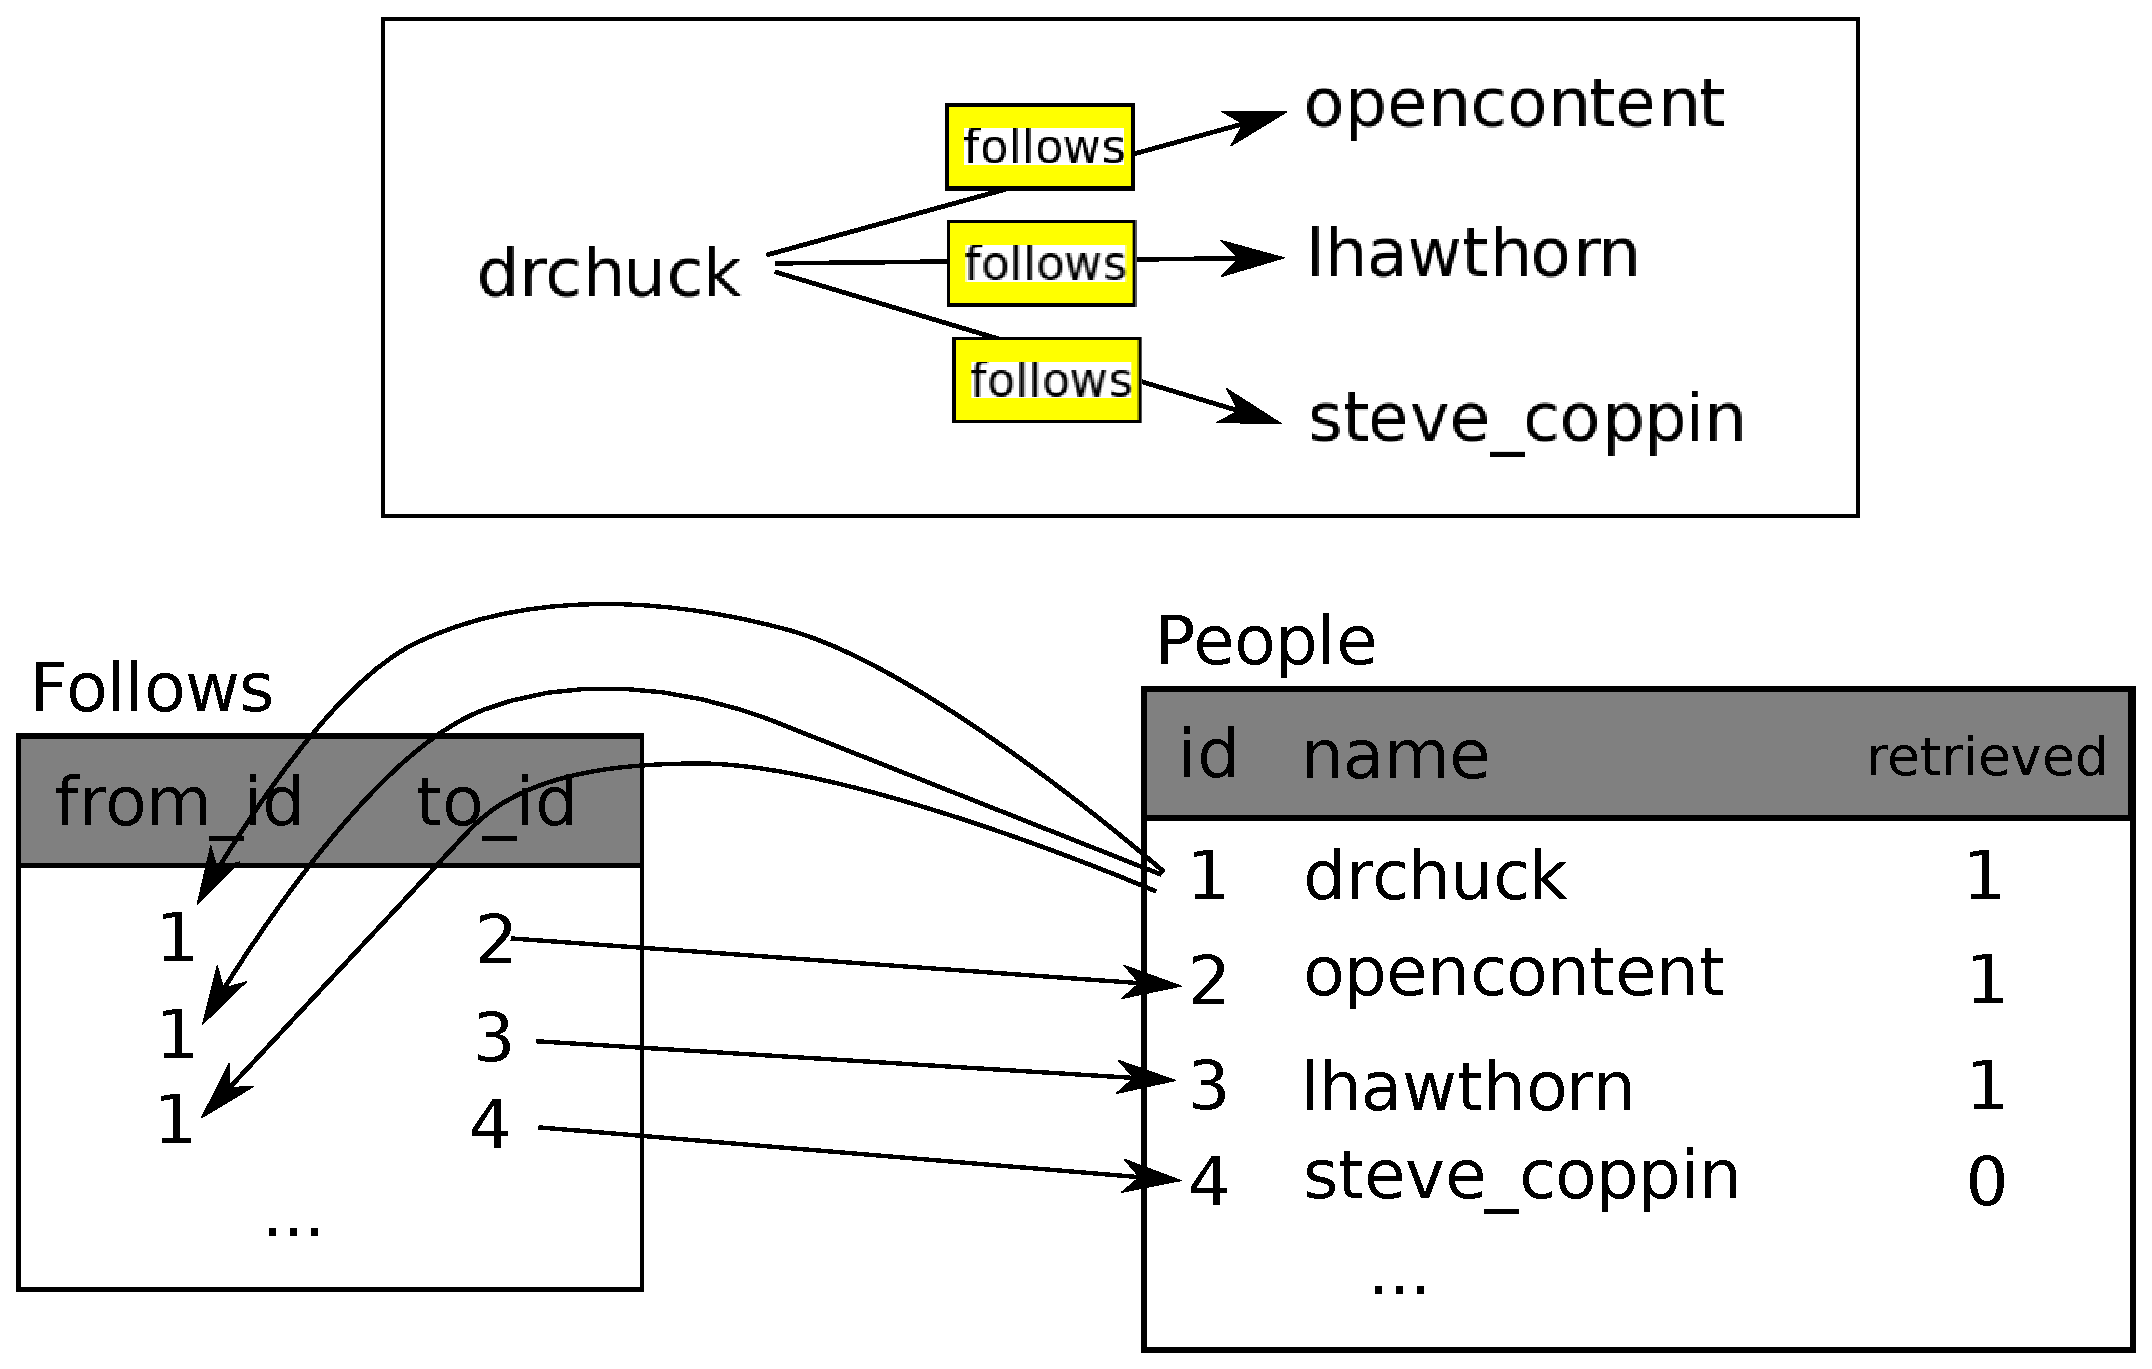
\includegraphics[height=2.50in]{figs2/twitter.eps}}
\afterfig


\section{Programming with multiple tables}

We will now re-do the Twitter spider program using two tables, the primary
keys, and the key references as described above.  Here is the code for 
the new version of the program:

\beforeverb
\begin{verbatim}
import sqlite3
import urllib
import xml.etree.ElementTree as ET

TWITTER_URL = 'http://api.twitter.com/l/statuses/friends/ACCT.xml'

conn = sqlite3.connect('twdata.db')
cur = conn.cursor()

cur.execute('''CREATE TABLE IF NOT EXISTS People 
    (id INTEGER PRIMARY KEY, name TEXT UNIQUE, retrieved INTEGER)''')
cur.execute('''CREATE TABLE IF NOT EXISTS Follows 
    (from_id INTEGER, to_id INTEGER, UNIQUE(from_id, to_id))''')

while True:
    acct = raw_input('Enter a Twitter account, or quit: ')
    if ( acct == 'quit' ) : break
    if ( len(acct) < 1 ) :
        cur.execute('''SELECT id,name FROM People 
            WHERE retrieved = 0 LIMIT 1''')
        try:
            (id, acct) = cur.fetchone()
        except:
            print 'No unretrieved Twitter accounts found'
            continue
    else:
        cur.execute('SELECT id FROM People WHERE name = ? LIMIT 1', 
            (acct, ) )
        try:
            id = cur.fetchone()[0]
        except:
            cur.execute('''INSERT OR IGNORE INTO People 
                (name, retrieved) VALUES ( ?, 0)''', ( acct, ) )
            conn.commit()
            if cur.rowcount != 1 : 
                print 'Error inserting account:',acct
                continue
            id = cur.lastrowid

    url = TWITTER_URL.replace('ACCT', acct)
    print 'Retrieving', url
    document = urllib.urlopen (url).read()
    tree = ET.fromstring(document)

    cur.execute('UPDATE People SET retrieved=1 WHERE name = ?', (acct, ) )

    countnew = 0
    countold = 0
    for user in tree.findall('user'):
        friend = user.find('screen_name').text
        cur.execute('SELECT id FROM People WHERE name = ? LIMIT 1', 
            (friend, ) )
        try:
            friend_id = cur.fetchone()[0]
            countold = countold + 1
        except:
            cur.execute('''INSERT OR IGNORE INTO People (name, retrieved) 
                VALUES ( ?, 0)''', ( friend, ) )
            conn.commit()
            if cur.rowcount != 1 :
                print 'Error inserting account:',friend
                continue
            friend_id = cur.lastrowid
            countnew = countnew + 1
        cur.execute('''INSERT OR IGNORE INTO Follows 
            (from_id, to_id) VALUES (?, ?)''', (id, friend_id) )
    print 'New accounts=',countnew,' revisited=',countold
    conn.commit()

cur.close()
\end{verbatim}
\afterverb
%
This program is starting to get a bit complicated, but it illustrates
the patterns that we need to use when we are
using integer keys to link tables. The basic patterns are:

\begin{enumerate}

\item Creating tables with primary keys and constraints.

\item When we have a logical key for a person (i.e. account
name) and we need the {\tt id} value for the person.
Depending on whether or not the person is already
in the {\tt People} table, we either need to: 
(1) look up the person in the {\tt People} table and 
retrieve the {\tt id} value for the person 
or (2) add the person the the {\tt People} table and get the 
{\tt id} value for the newly added row.

\item Insert the row that captures the ``follows'' relationship.

\end{enumerate}

We will cover each of these in turn.

\subsection{Constraints in database tables}

As we design our table structures, we can tell the database system 
that we would like it to enforce a few rules on us.   These rules
help us from making mistakes and introducing incorrect data into 
out tables.   When we create our tables:

\beforeverb
\begin{verbatim}
cur.execute('''CREATE TABLE IF NOT EXISTS People 
    (id INTEGER PRIMARY KEY, name TEXT UNIQUE, retrieved INTEGER)''')
cur.execute('''CREATE TABLE IF NOT EXISTS Follows 
    (from_id INTEGER, to_id INTEGER, UNIQUE(from_id, to_id))''')
\end{verbatim}
\afterverb
%
We indicate that the {\tt name} column in the {\tt People} table must be
{\tt UNIQUE}.   We also indicate that the combination of the two numbers
in each row of the {\tt Follows} table must be unique.  These constraints
keep us from making mistakes such as adding the same relationship more than
once.

We can take advantage of these constraints in the following code:

\beforeverb
\begin{verbatim}
cur.execute('''INSERT OR IGNORE INTO People (name, retrieved) 
    VALUES ( ?, 0)''', ( friend, ) )
\end{verbatim}
\afterverb
%
We add the {\tt OR IGNORE} clause to our {\tt INSERT} statement to indicate
that if this particular {\tt INSERT} would cause a violation of the
``{\tt name} must be unique'' rule, the database system is allowed to ignore the 
{\tt INSERT}.  We are using the database constraint as a safety net
to make sure we don't inadvertently do something incorrect.

Similarly, the following code ensures that we don't add the 
exact same {\tt Follows} relationship twice.

\beforeverb
\begin{verbatim}
cur.execute('''INSERT OR IGNORE INTO Follows 
    (from_id, to_id) VALUES (?, ?)''', (id, friend_id) )
\end{verbatim}
\afterverb
%
Again we simply tell the database to ignore our attempted 
{\tt INSERT} if it would violate the uniqueness constraint
that we specified for the {\tt Follows} rows.

\subsection{Retrieve and/or insert a record}

When we prompt the user for a Twitter account, if the account 
exists, we must look up its {\tt id} value.  If the account
does not yet exist in the {\tt People} table, we must insert 
the record and get the {\tt id} value from the inserted
row.

This is a very common pattern and is done twice in the program above.
This code shows how we look up the {\tt id} for a 
friend's account when we have extracted a \verb"screen_name"
from a {\tt user} node in the retrieved Twitter XML.

Since over time it will be increasingly likely that the account
will already be in the database, we first check to see if the
{\tt People} record exists using a {\tt SELECT} statement.

If all goes well\footnote{In general, when a sentence starts 
with ``if all goes well'' you will find that the code needs
to use try/except.} inside the {\tt try} section, we retrieve the
record using {\tt fetchone()} and then retrieve the
first (and only) element of the returned tuple and store it in 
\verb"friend_id".

If the {\tt SELECT} fails, the {\tt fetchone()[0]} code will fail
and control will transfer into the {\tt except} section.

\beforeverb
\begin{verbatim}
        friend = user.find('screen_name').text
        cur.execute('SELECT id FROM People WHERE name = ? LIMIT 1',
            (friend, ) )
        try:
            friend_id = cur.fetchone()[0]
            countold = countold + 1
        except:
            cur.execute('''INSERT OR IGNORE INTO People (name, retrieved) 
                VALUES ( ?, 0)''', ( friend, ) )
            conn.commit()
            if cur.rowcount != 1 :
                print 'Error inserting account:',friend
                continue
            friend_id = cur.lastrowid
            countnew = countnew + 1
\end{verbatim}
\afterverb
%
If we end up in the {\tt except} code, it simply means that the row
was not found so we must insert the row.  We use {\tt INSERT OR 
IGNORE} just to avoid errors and then call {\tt commit()} to 
force the database to really be updated.  After the write is done, we can 
check the {\tt cur.rowcount} to see how many rows were affected.  Since
we are attempting to insert a single row, if the number of 
affected rows is something other than one, it is an error.  

If the {\tt INSERT} is successful, we can look at {\tt cur.lastrowid} 
to find out what value the database assigned to the {\tt id} column in 
our newly created row.

\subsection{Storing the friend relationship}

Once we know the key value for both the Twitter user
and the friend in the XML, it is a simple matter to insert
the two numbers into the {\tt Follows} table
with the following code:

\beforeverb
\begin{verbatim}
cur.execute('INSERT OR IGNORE INTO Follows (from_id, to_id) VALUES (?, ?)',
    (id, friend_id) )
\end{verbatim}
\afterverb
%
Notice that we let the database take care of keeping us from ``double-inserting''
a relationship by creating the table with a uniqueness constraint and then
adding {\tt OR IGNORE} to our {\tt INSERT} statement.

Here is a sample execution of this program:
\beforeverb
\begin{verbatim}
Enter a Twitter account, or quit: 
No unretrieved Twitter accounts found
Enter a Twitter account, or quit: drchuck
Retrieving http://api.twitter.com/l/statuses/friends/drchuck.xml
New accounts= 100  revisited= 0
Enter a Twitter account, or quit: 
Retrieving http://api.twitter.com/l/statuses/friends/opencontent.xml
New accounts= 97  revisited= 3
Enter a Twitter account, or quit: 
Retrieving http://api.twitter.com/l/statuses/friends/lhawthorn.xml
New accounts= 97  revisited= 3
Enter a Twitter account, or quit: quit
\end{verbatim}
\afterverb
%
We started with the {\tt drchuck} account and then let the program
automatically pick the next two accounts to retrieve and add to 
our database.

The following is the first few rows in the {\tt People} 
and {\tt Follows} tables after this run is completed:
\beforeverb
\begin{verbatim}
People:
(1, u'drchuck', 1)
(2, u'opencontent', 1)
(3, u'lhawthorn', 1)
(4, u'steve_coppin', 0)
(5, u'davidkocher', 0)
295 rows.
Follows:
(1, 2)
(1, 3)
(1, 4)
(1, 5)
(1, 6)
300 rows.
\end{verbatim}
\afterverb
%
You can see the {\tt id}, {\tt name}, and {\tt visited} fields in the 
{\tt People} table and you see the numbers of both ends of 
the relationship {\tt Follows} table.   
In the {\tt People} table, we can see that the first three people
have been visited and their data has been retrieved.
The data in the {\tt Follows} table indicates that
{\tt drchuck} (user 1) is a friend to all of the people shown in the first
five rows.  This makes sense because
the first data we retrieved and stored was the Twitter friends of
{\tt drchuck}.  If you were to print more rows from the {\tt Follows} table,
you would see the friends of user two and three as well.

\section{Three kinds of keys}

Now that we have started building a data model putting our
data into multiple linked tables, and linking the rows in those
tables using {\bf keys}, we need to look at some terminology 
around keys.  There are generally three kinds of keys used 
in a database model.

\begin{itemize}

\item A {\bf logical key} is a key that the ``real world'' might use
to look up a row.   In our example data model, the {\tt name}
field is a logical key.  It is the screen name for the user 
and we indeed look up a user's row several times in the program
using the {\tt name} field.  You will often find that it makes
sense to add a {\tt UNIQUE} constraint to a logical key.  Since the 
logical key is how we look up a row from the outside world, it makes
little sense to allow multiple rows with the same value in the table.

\item A {\bf primary key} is usually a number that is assigned
automatically by the database.  It generally has no meaning outside
the program and is only used to link rows from different tables
together.  When we want to look up a row in a table, usually 
searching for the row using the primary key is the fastest 
way to find a row.  Since primary keys are integer numbers, they 
take up very little storage and can be compared or sorted very quickly.
In our data model, the {\tt id} field is an example of a primary key.

\item A {\bf foreign key} is usually a number that points to the primary key
of an associated row in a different table.  An example of a foreign
key in our data model is the \verb"from_id".  

\end{itemize}

We are using a
naming convention of always calling the primary key field name
{\tt id} and appending the suffix \verb"_id" to any field name
that is a foreign key.


\section{Using JOIN to retrieve data}

Now that we have followed the rules of database normalization
and have data separated into two tables, linked together using
primary and foreign keys, we need to be able to build a 
{\tt SELECT} that re-assembles the data across the tables.

SQL uses the {\tt JOIN} clause to re-connect these tables.  
In the {\tt JOIN} clause you specify the fields that are used 
to re-connect the rows between the tables.

The following is an example of a {\tt SELECT} with a 
{\tt JOIN} clause:

\beforeverb
\begin{verbatim}
SELECT * FROM Follows JOIN People 
    ON Follows.to_id = People.id WHERE Follows.from_id = 2
\end{verbatim}
\afterverb
%
The {\tt JOIN} clause indicates that the fields we are selecting
cross both the {\tt Follows} and {\tt People} tables.  The {\tt ON}
clause indicates how the two tables are to be joined.   Take the rows
from {\tt Follows} and append the row from {\tt People} where the
field \verb"from_id" in {\tt Follows} is the same the {\tt id} value
in the {\tt People} table.

\beforefig
\centerline{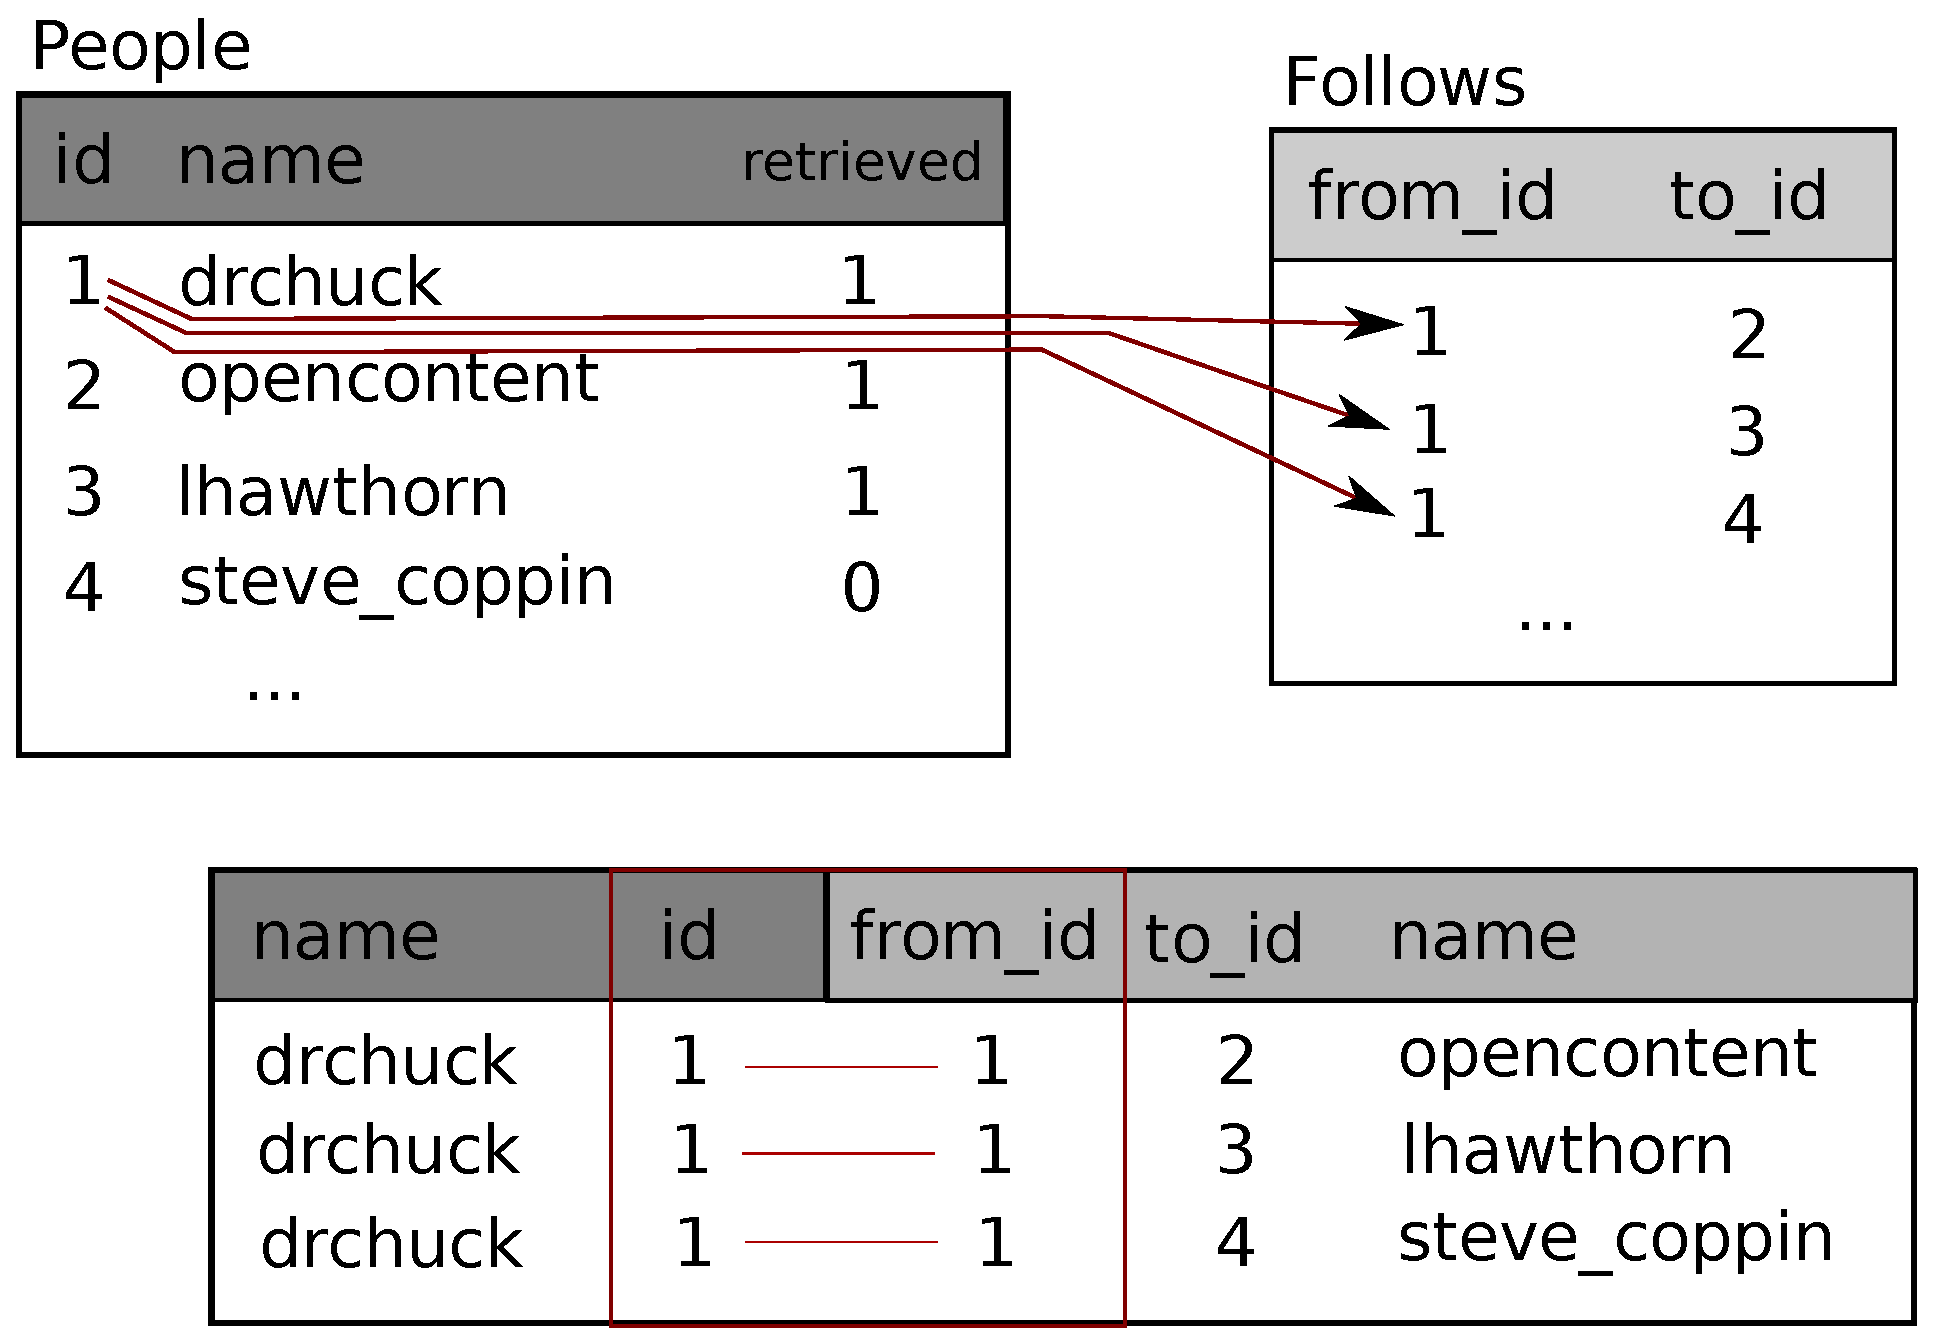
\includegraphics[height=2.50in]{figs2/join.eps}}
\afterfig

The result of the JOIN is to create extra-long ``meta-rows'' which have both 
the fields from {\tt People} and the matching fields from {\tt Follows}.
Where there is more than one match between the {\tt id} field from {\tt People}
and the \verb"from_id" from {\tt People}, then JOIN creates a meta-row 
for \emph{each} of the matching pairs of rows, duplicating data as needed.

The following code demonstrates the data that we will have in the 
database after the multi-table Twitter spider program (above) has
been run several times.

\beforeverb
\begin{verbatim}
import sqlite3

conn = sqlite3.connect('twdata.db')
cur = conn.cursor()

cur.execute('SELECT * FROM People')
count = 0
print 'People:'
for row in cur :
   if count < 5: print row
   count = count + 1
print count, 'rows.'

cur.execute('SELECT * FROM Follows')
count = 0
print 'Follows:'
for row in cur :
   if count < 5: print row
   count = count + 1
print count, 'rows.'

cur.execute('''SELECT * FROM Follows JOIN People 
    ON Follows.to_id = People.id WHERE Follows.from_id = 2''')
count = 0
print 'Connections for id=2:'
for row in cur :
   if count < 5: print row
   count = count + 1
print count, 'rows.'

cur.close()
\end{verbatim}
\afterverb
%
In this program, we first dump out the {\tt People}
and {\tt Follows} and then dump out a subset of the
data in the tables joined together.

Here is the output of the program:

\beforeverb
\begin{verbatim}
python twjoin.py 
People:
(1, u'drchuck', 1)
(2, u'opencontent', 1)
(3, u'lhawthorn', 1)
(4, u'steve_coppin', 0)
(5, u'davidkocher', 0)
295 rows.
Follows:
(1, 2)
(1, 3)
(1, 4)
(1, 5)
(1, 6)
300 rows.
Connections for id=2:
(2, 1, 1, u'drchuck', 1)
(2, 28, 28, u'cnxorg', 0)
(2, 30, 30, u'kthanos', 0)
(2, 102, 102, u'SomethingGirl', 0)
(2, 103, 103, u'ja_Pac', 0)
100 rows.
\end{verbatim}
\afterverb
%
You see the columns from the {\tt People} and {\tt Follows} tables and the last
set of rows is the result of the {\tt SELECT} with the {\tt JOIN} clause.

In the last select, we are looking for accounts that are friends of 
``opencontent'' (i.e. {\tt People.id=2}).

In each of the ``meta-rows'' in the last select, the first two columns are
from the {\tt Follows}
table followed by columns three through five from the {\tt People} table.  You can also
see that the second column (\verb"Follows.to_id") matches the third column
({\tt People.id}) in each of the joined-up ``meta-rows''.

\section{Summary}

This chapter has covered a lot of ground to give you an overview of the basics
of using a database in Python.   It is more complicated to write the code to use 
a database to store data than Python dictionaries or flat files so there is 
little reason to use a database unless your application truly needs the capabilities
of a database.  The situations where a database can be quite useful are: 
(1) when your application needs to make small many random updates within a large data set,
(2) when your data is so large it cannot fit in a dictionary and you need to 
look up information repeatedly, or
(3) you have a long-running process that you want to be able to stop 
and restart and retain the data from one run to the next.

You can build a simple database with a single table to suit many application 
needs, but most problems will require several tables and links/relationships
between rows in different tables.   When you start making links between 
tables, it is important to do some thoughful design and follow the 
rules of database normalization to make the best use of the database's
capabilities.  Since the primary motivation for using a database
is that you have a large amount of data to deal with, it is important
to model your data efficiently so your programs run as fast as possible.

\section{Debugging}

One common pattern when you are developing a Python program to connect to
an SQLite database will be to run a Python program and check the
results using the SQLite Database Browser.  The browser allows you 
to quickly check to see if your program is working properly.

You must be careful because SQLite takes care to keep two programs
from changing the same data at the same time.   For example, if
you open a database in the browser and make a change to the database
and have not yet pressed the ``save'' button in the browser, the 
browser ``locks'' the database file and keeping any other program
from accessing the file.  In particular, your Python program
will not be able to access the file if it is locked.

So a solution is to make sure to either close the dababase browser 
or use the {\bf File} menu to close the database in the browser
before you attempt to access the database from Python to avoid
the problem of your Python code failing because the database is
locked.

\section{Glossary}

\begin{description}

\item[attribute:] One of the values within a tuple.  More commonly
called a ``column'' or ``field''.
\index{attribute}

\item[constraint:] 
When we tell the database to enforce a rule on a field or a row
in a table.  A common constraint is to insist that there can be no
duplicate values in a particular field (i.e. all the values must be unique).
\index{constraint}

\item[cursor:] A cursor allows you to execute SQL commands in a database
and retrieve data from the database.  A cursor is similar to 
a socket or file handle for network connections and files respectively.
\index{cursor}

\item[database browser:] 
A piece of software that allows you to directly connect to a database 
and manipulate the database directly without writing a program.
\index{database browser}

\item[foreign key:] A numeric key that points to the primary key of 
a row in another table.  Foreign keys establish relationships between rows
stored in different tables.
\index{foreign key}

\item[index:] Additional data that the database software maintains as rows
are inserted into a table designed to make lookups very fast.
\index{index}

\item[logical key:] A key that the ``outside world'' uses to look up a particular
row.  For example in a table of user accounts, a person's E-Mail address
might be a good candidate as the logical key for the user's data. 
\index{logical key}

\item[normalization:] Designing a data model so that no data
is replicated.  We store each item of data at one place in the database
and reference it elsewhere using a foreign key.
\index{normalization}
\index{database normalization}

\item[primary key:] A numeric key assigned to each row that is used to 
refer to one row in a table from another table.  Often the database
is configured to automatically assign primary keys as rows are inserted.
\index{primary key}

\item[relation:] An area within a database that contains tuples and 
attributes.  More typically called a ``table''.
\index{relation}

\item[tuple:] A single entry in a database table that is a set 
of attributes.  More typically called ``row''.
\index{tuple}

\end{description}

\section{Exercises}

\begin{ex}
Retrieve the following file \url{http://www.py4inf.com/code/wikidata.db} 
and use the SQLite browser to figure out how many tables
are in the datbase and list the fields for each of the tables including the
type of the field.  One of the fields is a type that is not described in 
this chapter.  Use the SQLite online documentation to describe the
purpose of that type of data?
\end{ex}

\chapter{Regular Expressions}

So far we have been reading through files, looking for patterns and extracting various bits of lines that we find interesting.  We have been using string methods like {\tt split} and {\tt find} and using lists and string slicing to extract portions of the lines.
\index{regular expressons}
\index{regex}
\index{re module}

This task of searching and extracting is so common that Python has a very powerful library called {\bf regular expressions} that handles many of these tasks quite elegantly.  The reason we have not introduced regular expressions earlier in the book because while they are very powerful, they are a little complicated and their syntax takes a little getting used to. 

Regular expressions are almost their own little programming language for searching and parsing strings.  As a matter of fact, entire books have been written on the topic of regular expressions.  In this chapter, we will only cover the basics of regular expressions.  For more detail on regular expressions, see:

\url{http://en.wikipedia.org/wiki/Regular_expression}

\url{http://docs.python.org/library/re.html}

The regular expression library must be imported into your program before you can use it.  The simplest use of the regular expression library is the {\tt search()} function.  The following program demonstrates a trivial use of the search function.
\index{regex!search}

\beforeverb
\begin{verbatim}
import re
hand = open('mbox-short.txt')
for line in hand:
    line = line.rstrip()
    if re.search('From:', line) :
        print line
\end{verbatim}
\afterverb
%
We open the file, loop through each line and use the regular expression {\tt search()} to only print out lines that contain the string ``From:''.   This program does not use the real power of regular expressions since we could have just as easily used {\tt line.find()} to accomplish the same result.
\index{string!find}

The power of the regular expressions comes we add to special characters to the search string that allow us to more precisely control which lines match the string.  Adding these special characters to our regular expression allow us to do sophisticated matching and extraction while writing very little code.

For example, if we wanted to only match lines where ``From:'' was at the beginning of the line, we could add the caret character which a special character in regular expressions that matches the beginning of a line and change our application as follows:

\beforeverb
\begin{verbatim}
import re
hand = open('mbox-short.txt')
for line in hand:
    line = line.rstrip()
    if re.search('^From:', line) :
        print line
\end{verbatim}
\afterverb
%
Now we will only match lines that {\em start with} the string ``From:''.  This is still a very simple example that we could have done equivalently with the {\tt startswith()} method from the string library.  But it serves to introduce the notion that regular expressions contain special action characters that give us more control as to what will match the regular expression.
\index{string!startswith}

\section{Character Matching in Regular Expressions}

There are a number of other special characters that let us build even more powerful regular expressions.  The most commonly used special character is the period character which matches any character.
\index{wild card}
\index{regex!wild card}

In the following example, the regular expression ``F..m:'' would match any of the strings ``From:'', ``Fxxm:'', ``F12m:'', or ``F!@m:'' since the period characters in the regular expression match any character.

\beforeverb
\begin{verbatim}
import re
hand = open('mbox-short.txt')
for line in hand:
    line = line.rstrip()
    if re.search('^F..m:', line) :
        print line
\end{verbatim}
\afterverb
%
This is particularly powerful when combined with the ability to indicate that a character can be repeated any number of times using the ``*'' or ``+'' characters in your regular expression.   These special characters mean that instead of matching a single character in the search string they match zero-or-more in the case of the asterisk or one-or-more of the characters in the case of the plus sign.

We can further narrow down the lines that we match using a repeated {\bf wild card} character in the following example:

\beforeverb
\begin{verbatim}
import re
hand = open('mbox-short.txt')
for line in hand:
    line = line.rstrip()
    if re.search('^From:.+@', line) :
        print line
\end{verbatim}
\afterverb
%
The search string ``\verb"^"From:.+@'' will successfully match lines that start with ``From:'' followed by one or more characters ``.+'' followed by an at-sign.  So this will match the following line:

{\tt
{\bf From:}\underline{ stephen.marquard}{\bf @}uct.ac.za
}

You can think of the ``.+'' wildcard as expanding to match all the characters between the 
colon character and the at-sign.  


{\tt
{\bf From:}\underline{.+}{\bf @}
}

It is good to think of the plus and asterisk characters as ``pushy''.  For example the following string would match the last at-sign in the string as the ``.+'' pushes outwards as shown below:

{\tt
{\bf From:}\underline{ stephen.marquard@uct.ac.za, csev@umich.edu, and cwen}{\bf @}iupui.edu
}

It is possible to tell an asterisk or plus-sign not to be so ``greedy'' by adding 
another character.   See the detailed dcumentation for information on turning off the 
greedy behavior.
\index{greedy}

\section{Extracting Data Using Regular Expressions}

If we want to extract data from a string in Python we can use the {\tt findall()} method to extract all of the substrings which match a regular expression.  Lets use the example of wanting to extract anything that looks like an E-Mail address from any line regardless of format.  For example, we want to pull the e-mail addresses from each of the following lines:

\beforeverb
\begin{verbatim}
From stephen.marquard@uct.ac.za Sat Jan  5 09:14:16 2008
Return-Path: <postmaster@collab.sakaiproject.org>
          for <source@collab.sakaiproject.org>;
Received: (from apache@localhost)
Author: stephen.marquard@uct.ac.za
\end{verbatim}
\afterverb
%
We don't want to write code for each of the types of lines, splitting and slicing differently for each line.  This following program uses {\tt findall()} to find the lines with E-Mail addresses in them and extract one or more addresses from each of those lines.
\index{findall}
\index{regex!findall}

\beforeverb
\begin{verbatim}
import re
s = 'Hello from csev@umich.edu to cwen@iupui.edu about the meeting @2PM'
lst = re.findall('\S+@\S+', s)
print lst
\end{verbatim}
\afterverb
%
The {\tt findall()} method searches the string in the second argument and returns a list of all of the strings that look like E-Mail addresses.   We are using a special character that indicates a non-whitespace character ({\textbackslash}S). 

The output of the program would be:

\beforeverb
\begin{verbatim}
['csev@umich.edu', 'cwen@iupui.edu']
\end{verbatim}
\afterverb
%
Translating the regular expression, we are looking for substrings that have at least one non-whitespace character, followed by an at-sign, followed by at least one more non-white space characters.  Also, the ``{\textbackslash}S+'' matches as many non-whitespace characters as possible (this is called {\bf ``greedy''} matching in regular expressions).  

The regular expression would match twice (csev@umich.edu and cwen@iupui.edu) but it would not match the string ``@2PM'' because there are no non-blank characters {\em before} the at-sign.  
We can use this regular expression in a program to read all the lines in a file and print out anything that looks like an E-Mail address as follows:

\beforeverb
\begin{verbatim}
import re
hand = open('mbox-short.txt')
for line in hand:
    line = line.rstrip()
    x = re.findall('\S+@\S+', line)
    if len(x) > 0 :
        print x
\end{verbatim}
\afterverb
%
We read each line and then extract all the substrings that match our regular expression.  Since {\tt findall()} returns a list, we simple check if the number of elements in our returned list is more than zero to print only lines where we found at least one substring that looks like an E-Mail address.

If we run the program on {\tt mbox.txt} we get the following output:

\beforeverb
\begin{verbatim}
['wagnermr@iupui.edu']
['cwen@iupui.edu']
['<postmaster@collab.sakaiproject.org>']
['<200801032122.m03LMFo4005148@nakamura.uits.iupui.edu>']
['<source@collab.sakaiproject.org>;']
['<source@collab.sakaiproject.org>;']
['<source@collab.sakaiproject.org>;']
['apache@localhost)']
['source@collab.sakaiproject.org;']
\end{verbatim}
\afterverb
%
Some of our E-mail addresses have incorrect characters like ``\verb"<"'' or ``;'' at the beginning or end.   Lets declare that we are only interested in the portion of the string that starts and ends with a letter or a number.

To do this, we use another feature of regular expressions.  Square brackets are used to indicate a set of multiple acceptable characters we are willing to consider matching.  In a sense, the ``{\textbackslash}S'' is asking to match the set of ``non-whitespace characters''.  Now we will be a little more explicit in terms of the characters we will match.

Here is our new regular expression:

\beforeverb
\begin{verbatim}
[a-zA-Z0-9]\S*@\S*[a-zA-Z]
\end{verbatim}
\afterverb
%
This is getting a little complicated and you can begin to see why regular expressions are their own little language unto themselves.  Translating this regular expression, we are looking for substrings that start with a {\em single} lowercase letter, upper case letter, or number ``[a-zA-Z0-9]'' followed by zero or more non blank characters ``{\textbackslash}S*'', followed by an at-sign, followed by zero or more non-blank characters ``{\textbackslash}S*'' followed by an upper or lower case letter.  Note that we switched from ``+'' to ``*'' to indicate zero-or-more non-blank characters since ``[a-zA-Z0-9]'' is already one non-blank character.   Remember that the ``*'' or ``+'' applies to the single character immediately to the left of the plus or asterisk.
\index{regex!character sets(brackets)}

If we use this expression in our program, our data is much cleaner:

\beforeverb
\begin{verbatim}
import re
hand = open('mbox-short.txt')
for line in hand:
    line = line.rstrip()
    x = re.findall('[a-zA-Z0-9]\S+@\S+[a-zA-Z]', line)
    if len(x) > 0 :
        print x
\end{verbatim}
\afterverb
%
\beforeverb
\begin{verbatim}
…
['wagnermr@iupui.edu']
['cwen@iupui.edu']
['postmaster@collab.sakaiproject.org']
['200801032122.m03LMFo4005148@nakamura.uits.iupui.edu']
['source@collab.sakaiproject.org']
['source@collab.sakaiproject.org']
['source@collab.sakaiproject.org']
['apache@localhost']
\end{verbatim}
\afterverb
%
Notice that on the ``source@collab.sakaiproject.org'' lines, our regular expression eliminated two letters at the end of the string (``\verb">";'').  This is because when we append ``[a-zA-Z]'' to the end of our regular expression, we are demanding that whatever string the regular expression parser finds, it must end with a letter.   So when it sees the ``\verb">"'' after ``sakaiproject.org\verb">";'' it simply stops at the last ``matching'' letter it found (i.e. the ``g'' was the last good match).

Also note that the output of the program is a Python list that has a string as the single element in the list.

\section{Combining Searching and Extracting}

Lets say we want to find numbers on lines that start with the string ``X-'' like the following.:

\beforeverb
\begin{verbatim}
X-DSPAM-Confidence: 0.8475
X-DSPAM-Probability: 0.0000  
\end{verbatim}
\afterverb
%
We don't just want any floating point point numbers from any lines.  We only to extract numbers from lines that have the above syntax.

We can construct the following regular expression to select the lines:

\beforeverb
\begin{verbatim}
^X-.*: [0-9.]+
\end{verbatim}
\afterverb
%
Translating this, we are saying, we want lines that start with ``X-'' followed by zero or more characters ``.*'' followed by a colon (``:'') and then a space.  After the space we are looking for one or more characters that are either a digit (0-9) or a period ``[0-9.]+''.  Note that in between the square braces, the period matches an actual period (i.e. it is not a wildcard between the square brackets).

This is a very tight expression that will pretty much match only the lines we are interested in as follows:

\beforeverb
\begin{verbatim}
import re
hand = open('mbox-short.txt')
for line in hand:
    line = line.rstrip()
    if re.search('^X\S*: [0-9.]+', line) :
        print line
\end{verbatim}
\afterverb
%
When we run the program, we see the data nicely filtered to show 
only the lines we are looking for.

\beforeverb
\begin{verbatim}
X-DSPAM-Confidence: 0.8475
X-DSPAM-Probability: 0.0000
X-DSPAM-Confidence: 0.6178
X-DSPAM-Probability: 0.0000
\end{verbatim}
\afterverb
%
But now we have to solve the problem of extracting the numbers using {\tt split}.  While it would be simple enough to use {\tt split}, we can use another feature of regular expressions to both search and parse the line at the same time.
\index{string!split}

Parentheses are another special character in regular expressions.  When you add parentheses to a regular expression they are ignored when matching the string, but when you are using {\tt findall()}, parentheses indicates that you while you want the whole expression to match, you only are interesed in extracting a portion of the substring that matches the regular expression.  
\index{regex!parentheses}
\index{parentheses!regular expression}

So we make the following change to our program:

\beforeverb
\begin{verbatim}
import re
hand = open('mbox-short.txt')
for line in hand:
    line = line.rstrip()
    x = re.findall('^X\S*: ([0-9.]+)', line)
    if len(x) > 0 :
        print x
\end{verbatim}
\afterverb
%
Instead of calling {\tt search()}, we add a parentheses around the part of the regular expression that represents the floating point number to indicate we only want {\tt findall()} to give us back the floating point number portion of the matching string.

The output from this program is as follows:

\beforeverb
\begin{verbatim}
['0.8475']
['0.0000']
['0.6178']
['0.0000']
['0.6961']
['0.0000']
..
\end{verbatim}
\afterverb
%
The numbers are still in a list and need to be converted from strings to floating point but we have used the power of regular expressions to both search and extract the information we found interesting.

As another example of this technique, if 
you look at the file there are a number of lines of the form:

\beforeverb
\begin{verbatim}
Details: http://source.sakaiproject.org/viewsvn/?view=rev&rev=39772
\end{verbatim}
\afterverb
%
Lets say, we wanted to extract all of the revision numbers (the integer number at the end of these lines) using the same technique as above.   We could write the following program:

\beforeverb
\begin{verbatim}
import re
hand = open('mbox-short.txt')
for line in hand:
    line = line.rstrip()
    x = re.findall('^Details:.*rev=([0-9.]+)', line)
    if len(x) > 0:
        print x
\end{verbatim}
\afterverb
%
Translating our regular expression, we are looking for lines that start with ``Details:', followed by any any number of characters ``.*'' followed by ``rev='' and then by one or more digits.   We want lines that match the entire expression but we only want to extract the integer number at the end of the line so we surround ``[0-9]+'' with parentheses.  

When we run the program, we get the following output:

\beforeverb
\begin{verbatim}
['39772']
['39771']
['39770']
['39769']
...
\end{verbatim}
\afterverb
%
Remember that the ``[0-9]+'' is ``greedy'' and it tries to make as large a string of digits as possible before extracting those digits.  This ``greedy'' behavior is why we get all five digits for each number.  The regular expression library expands in both directions until it counters a non-digit, the beginning, or the end of a line.

Now lets use regular expressions to re-do an exercise from earlier in the book where we were interested in the time of day of each mail message.   We looked for lines of the form:

\beforeverb
\begin{verbatim}
From stephen.marquard@uct.ac.za Sat Jan  5 09:14:16 2008
\end{verbatim}
\afterverb
%
And wanted to extract the hour of the day for each line.  Previously we did this with two calls to {\tt split}.  First the line was split into words and then we pulled out the fifth word and split it again on the colon character to pull out the two characters we were interested in.

% Add a section on the notion of brittle code
While this worked, it actually results in pretty brittle code that is assuming the lines are nicely formatted.  If you were to add enough error checking (or a big try/except block) to insure that your program never failed when presented with incorrectly formatted lines, the code would balloon to 10-15 lines of code that was pretty hard to read.

We can do this far simpler with the following regular expression:

\beforeverb
\begin{verbatim}
^From .* [0-9][0-9]:
\end{verbatim}
\afterverb
%
The translation of this regular expression is that we are looking for lines that start with ``From '' (note the space) followed by any number of characters ``.*'' followed by a space followed by two digits ``[0-9][0-9]'' followed by a colon character.  This is the definition of the kinds of lines we are looking for.  

In order to pull out only the hour using {\tt findall()}, we add parentheses around the two digits as follows:

\beforeverb
\begin{verbatim}
^From .* ([0-9][0-9]):
\end{verbatim}
\afterverb
%
This results in the following program:

\beforeverb
\begin{verbatim}
import re
hand = open('mbox-short.txt')
for line in hand:
    line = line.rstrip()
    x = re.findall('^From .* ([0-9][0-9]):', line)
    if len(x) > 0 : print x
\end{verbatim}
\afterverb
%
When the program runs, it produces the following output:

\beforeverb
\begin{verbatim}
['09']
['18']
['16']
['15']
…
\end{verbatim}
\afterverb
%
\section{Summary}

While this only scratched the surface of regular expressions, we have learned a bit about the language of regular expressions.  They are search strings that have special characters in them that communicate your wishes to the regular expression system as to what defines ``matching'' and what is extracted from the matched strings.  Here are some of those specal characters and character sequences:

\verb"^" \newline
Matches the beginning of the line.

\$ \newline
Matches the end of the line.

. \newline
Matches any character (a wildcard).

{\textbackslash}s \newline
Matches a whitespace character.

{\textbackslash}S \newline
Matches a non-whitespace character (opposite of {\textbackslash}s).

* \newline
Applies to the immediately preceding character and indicates to match zero or more of the preceding character.

+ \newline
Applies to the immediately preceding character and indicates to match zero or more of the preceding character.

[abc] \newline
Matches a single character as long as that character is in the specified set.  In this example, it would match ``a'', ``b'', or ``c'' but no other characters.

[a-z0-9] \newline
You can specify ranges of characters using the minus sign.  This example is a single character that must be a lower case letter or a digit.

[\verb"^"A-Za-z] \newline
When the first character in the set notation is a caret, it inverts the logic.  This example matches a single character that is anything {\em other than} an upper or lower case character.

( ) \newline
When parentheses are added to a regular expression, they are ignored for the purpose of matching, but allow you to extract a particular subset of the matched string rather than the whole string when using {\tt findall()}.

{\textbackslash}b \newline
Matches the empty string, but only at the start or end of a word.

{\textbackslash}B \newline
Matches the empty string, but not at the start or end of a word.

{\textbackslash}d \newline
Matches any decimal digit; equivalent to the set [0-9].

{\textbackslash}D \newline
Matches any non-digit character; equivalent to the set [\verb"^"0-9].

\section{Bonus Section for UNIX Users}

Support for searching files using regular expressions was built into the UNIX operating since the 1960's and it is avaiable in nearly all programming languages in one form or another.

As a matter of fact, there is a command-line program built into UNIX called {\bf grep} (Generalized Regular Expression Parser) that does pretty much the same as the {\tt search()} examples in this chapter.  So if you have a Macintosh or Linux system, you can try the following commands in your command line window.

\beforeverb
\begin{verbatim}
$ grep '^From:' mbox-short.txt
From: stephen.marquard@uct.ac.za
From: louis@media.berkeley.edu
From: zqian@umich.edu
From: rjlowe@iupui.edu
\end{verbatim}
\afterverb
%
This tells {\tt grep} to show you lines that start with the string ``From:'' in the file {\tt mbox-short.txt}.   If you experiment with the {\tt grep} command a bit and read the documentation for {\tt grep}, you will find some subtle difference between the regular expression support in Python and the regular expression support in {\tt grep}.  As an example, {\tt grep} does not support the non-blank character ``{\textbackslash}S'' so you will need to use the slightly more complex set notation ``[\verb"^" ]''- which simply means - match a character that is anything other than a space.

\section{Debugging}

Python has some simple and rudimentary built-in documentation that can be quite helpful if you need a quick refresher to trigger your memory about the exact name of a particular method.   This documentation can be viewed in the Python interpreter in interactive mode.

You can bring up an interactive help system using {\tt help()}.

\beforeverb
\begin{verbatim}
>>> help()

Welcome to Python 2.6!  This is the online help utility.

If this is your first time using Python, you should definitely check out
the tutorial on the Internet at http://docs.python.org/tutorial/.

Enter the name of any module, keyword, or topic to get help on writing
Python programs and using Python modules.  To quit this help utility and
return to the interpreter, just type "quit".

To get a list of available modules, keywords, or topics, type "modules",
"keywords", or "topics".  Each module also comes with a one-line summary
of what it does; to list the modules whose summaries contain a given word
such as "spam", type "modules spam".

help> modules
\end{verbatim}
\afterverb
%
If you know what module you want to use, you can sue the {\tt dir()} command to find the methods in the module as follows:

\beforeverb
\begin{verbatim}
>>> import re
>>> dir(re)
[.. 'compile', 'copy_reg', 'error', 'escape', 'findall', 
'finditer', 'match', 'purge', 'search', 'split', 'sre_compile', 
'sre_parse', 'sub', 'subn', 'sys', 'template']
\end{verbatim}
\afterverb
%
You can also get a small amount of documentation on a particular method using the dir command.

\beforeverb
\begin{verbatim}
>>> help (re.search)
Help on function search in module re:

search(pattern, string, flags=0)
    Scan through string looking for a match to the pattern, returning
    a match object, or None if no match was found.
>>> 
\end{verbatim}
\afterverb
%
The built in documentation is not very extensive, but it can be helpful when you are in a hurry
or don't have access to a web browser or search engine.

\section{Glossary}

\begin{description}

\item{brittle code:}
Code that works when the input data is in a particular format but prone to breakage
if there is some deviation from the correct format.  We call this ``brittle code'' 
because it is easily broken.

\item{greedy matching:}
The notion that the ``+'' and ``*'' characters in a regular expression expand outward to match the largest possible string.
\index{greedy}
\index{greedy matching}

\item{grep:}
A command available in most UNIX systems that searches through text files looking for lines that match regular expressions.  The command name stands for "Generalized Regular Expression Parser".
\index{grep}

\item{regular expression:}
A language for expressing more complex search strings.  A regular expression may contain special characters that indicate that a search only matches at the beginning or end of a line or many other similar capabilities.

\item{wild card:}
A special character that matches any character.   In regular expressions the wild card character is the period character.
\index{wild card}

\end{description}

\section{Exercises}

\begin{ex}
Write a simple program to simulate the operation of the the {\tt grep} command 
on UNIX.  Ask the user to enter a regular expression and count the number
of lines that matched the regular expression:

\beforeverb
\begin{verbatim}
$ python grep.py
Enter a regular expression: ^Author
mbox.txt had 1798 lines that matched ^Author

$ python grep.py
Enter a regular expression: ^X-
mbox.txt had 14368 lines that matched ^X-

$ python grep.py
Enter a regular expression: java$
mbox.txt had 4218 lines that matched java$
\end{verbatim}
\afterverb
%
\end{ex}

\begin{ex}
Write a program to look for lines of the form

\verb"New Revision: 39772"

And extract the number from each of the lines using a regular expression
and the {\tt findall()} method.  Compute the average of the numbers and 
print out the average.
\end{ex}

% For now, we will produce without the additional chapters
% % LaTeX source for ``Python for Informatics: Exploring Information''
% Copyright (c)  2010  Charles R. Severance

% Permission is granted to copy, distribute and/or modify this
% document under the terms of the 
% 
% Creative Commons Attribution 3.0 - Share Alike Unported
% (or a later CC-SA) license

% http://creativecommons.org/licenses/by-sa/3.0/

\chapter{Advanced functions}
\label{fruitchap}

\section{Return values}
\index{return value}

Some of the built-in functions we have used, such as the math
functions, produce results.  Calling the function generates a
value, which we usually assign to a variable or use as part of an
expression.

\beforeverb
\begin{verbatim}
e = math.exp(1.0)
height = radius * math.sin(radians)
\end{verbatim}
\afterverb
%
All of the functions we have written so far are void; they print
something or move turtles around, but their return value is {\tt
None}.

In this chapter, we are (finally) going to write fruitful functions.
The first example is {\tt area}, which returns the area of a circle
with the given radius:

\beforeverb
\begin{verbatim}
def area(radius):
    temp = math.pi * radius**2
    return temp
\end{verbatim}
\afterverb
%
We have seen the {\tt return} statement before, but in a fruitful
function the {\tt return} statement includes
an expression.  This statement means: ``Return immediately from
this function and use the following expression as a return value.''
The expression can be arbitrarily complicated, so we could
have written this function more concisely:

\index{return statement}
\index{statement!return}

\beforeverb
\begin{verbatim}
def area(radius):
    return math.pi * radius**2
\end{verbatim}
\afterverb
%
On the other hand, {\bf temporary variables} like {\tt temp} often make
debugging easier.

\index{temporary variable}
\index{variable!temporary}

Sometimes it is useful to have multiple return statements, one in each
branch of a conditional:

\beforeverb
\begin{verbatim}
def absolute_value(x):
    if x < 0:
        return -x
    else:
        return x
\end{verbatim}
\afterverb
%
Since these {\tt return} statements are in an alternative conditional,
only one will be executed.

As soon as a return statement executes, the function
terminates without executing any subsequent statements.
Code that appears after a {\tt return} statement, or any other place
the flow of execution can never reach, is called {\bf dead code}.

\index{dead code}

In a fruitful function, it is a good idea to ensure
that every possible path through the program hits a
{\tt return} statement.  For example:

\beforeverb
\begin{verbatim}
def absolute_value(x):
    if x < 0:
        return -x
    if x > 0:
        return x
\end{verbatim}
\afterverb
%
This function is incorrect because if {\tt x} happens to be 0,
neither condition is true, and the function ends without hitting a
{\tt return} statement.  If the flow of execution gets to the end
of a function, the return value is {\tt None}, which is not
the absolute value of 0.

\index{None special value}
\index{special value!None}

\beforeverb
\begin{verbatim}
>>> print absolute_value(0)
None
\end{verbatim}
\afterverb
%
By the way, Python provides a built-in function called 
{\tt abs} that computes absolute values.

\index{abs function}
\index{function!abs}

\begin{ex}

\index{compare function}
\index{function!compare}

Write a {\tt compare} function
that returns {\tt 1} if {\tt x > y},
{\tt 0} if {\tt x == y}, and {\tt -1} if {\tt x < y}.
\end{ex}

\section{Tuples as return values}

\index{tuple}
\index{value!tuple}
\index{return value!tuple}
\index{function, tuple as return value}

Strictly speaking, a function can only return one value, but
if the value is a tuple, the effect is the same as returning
multiple values.  For example, if you want to divide two integers
and compute the quotient and remainder, it is inefficient to
compute {\tt x/y} and then {\tt x\%y}.  It is better to compute
them both at the same time.

\index{divmod}

The built-in function {\tt divmod} takes two arguments and
returns a tuple of two values, the quotient and remainder.
You can store the result as a tuple:

\beforeverb
\begin{verbatim}
>>> t = divmod(7, 3)
>>> print t
(2, 1)
\end{verbatim}
\afterverb
%
Or use tuple assignment to store the elements separately:

\index{tuple assignment}
\index{assignment!tuple}

\beforeverb
\begin{verbatim}
>>> quot, rem = divmod(7, 3)
>>> print quot
2
>>> print rem
1
\end{verbatim}
\afterverb
%
Here is an example of a function that returns a tuple:

\beforeverb
\begin{verbatim}
def min_max(t):
    return min(t), max(t)
\end{verbatim}
\afterverb
%
{\tt max} and {\tt min} are built-in functions that find
the largest and smallest elements of a sequence.  \verb"min_max"
computes both and returns a tuple of two values.

\index{max function}
\index{function!max}
\index{min function}
\index{function!min}


\section{Variable-length argument tuples}

\index{variable-length argument tuple}
\index{argument!variable-length tuple}
\index{gather}
\index{parameter!gather}
\index{argument!gather}

Functions can take a variable number of arguments.  A parameter
name that begins with {\tt *} {\bf gathers} arguments into
a tuple.  For example, {\tt printall}
takes any number of arguments and prints them:

\beforeverb
\begin{verbatim}
def printall(*args):
    print args
\end{verbatim}
\afterverb
%
The gather parameter can have any name you like, but {\tt args} is
conventional.  Here's how the function works:

\beforeverb
\begin{verbatim}
>>> printall(1, 2.0, '3')
(1, 2.0, '3')
\end{verbatim}
\afterverb
%
You can combine the gather operator with required and positional
arguments:

\beforeverb
\begin{verbatim}
def pointless(required, optional=0, *args):
    print required, optional, args
\end{verbatim}
\afterverb
%
Run this function with 1, 2, 3 and 4 or more arguments and
make sure you understand what it does.

\index{scatter}
\index{argument scatter}

The complement of gather is {\bf scatter}.  If you have a
sequence of values and you want to pass it to a function
as multiple arguments, you can use the {\tt *} operator.
For example, {\tt divmod} takes exactly two arguments; it
doesn't work with a tuple:

\index{TypeError}
\index{exception!TypeError}

\beforeverb
\begin{verbatim}
>>> t = (7, 3)
>>> divmod(t)
TypeError: divmod expected 2 arguments, got 1
\end{verbatim}
\afterverb
%
But if you scatter the tuple, it works:

\beforeverb
\begin{verbatim}
>>> divmod(*t)
(2, 1)
\end{verbatim}
\afterverb
%

\begin{ex}
Many of the built-in functions use
variable-length argument tuples.  For example, {\tt max}
and {\tt min} can take any number of arguments:

\index{max function}
\index{function!max}
\index{min function}
\index{function!min}

\beforeverb
\begin{verbatim}
>>> max(1,2,3)
3
\end{verbatim}
\afterverb
%
But {\tt sum} does not.

\index{sum function}
\index{function!sum}

\beforeverb
\begin{verbatim}
>>> sum(1,2,3)
TypeError: sum expected at most 2 arguments, got 3
\end{verbatim}
\afterverb
%
Write a function called {\tt sumall} that takes any number
of arguments and returns their sum.

\end{ex}



\section{Variables and parameters are local}
\index{local variable}
\index{variable!local}

When you create a variable inside a function, it is {\bf local},
which means that it only
exists inside the function.  For example:

\index{parentheses!parameters in}

\beforeverb
\begin{verbatim}
def cat_twice(part1, part2):
    cat = part1 + part2
    print_twice(cat)
\end{verbatim}
\afterverb
%
This function takes two arguments, concatenates them, and prints
the result twice.  Here is an example that uses it:

\index{concatenation}

\beforeverb
\begin{verbatim}
>>> line1 = 'Bing tiddle '
>>> line2 = 'tiddle bang.'
>>> cat_twice(line1, line2)
Bing tiddle tiddle bang.
Bing tiddle tiddle bang.
\end{verbatim}
\afterverb
%
When \verb"cat_twice" terminates, the variable {\tt cat}
is destroyed.  If we try to print it, we get an exception:

\index{NameError}
\index{exception!NameError}

\beforeverb
\begin{verbatim}
>>> print cat
NameError: name 'cat' is not defined
\end{verbatim}
\afterverb
%
Parameters are also local.
For example, outside \verb"print_twice", there is no
such thing as {\tt bruce}.

\index{parameter}

\section{Global variables}

\index{global variable}
\index{variable!global}

In the previous example, {\tt known} is created outside the function,
so it belongs to the special frame called \verb"__main__".
Variables in \verb"__main__" are sometimes called {\bf global}
because they can be accessed from any function.  Unlike local
variables, which disappear when their function ends, global variables
persist from one function call to the next.

\index{flag}

It is common to use global variables for {\bf flags}; that is, 
boolean variables that indicate (``flag'') whether a condition
is true.  For example, some programs use
a flag named {\tt verbose} to control the level of detail in the
output:

\beforeverb
\begin{verbatim}
verbose = True

def example1():
    if verbose:
        print 'Running example1'
\end{verbatim}
\afterverb
%
If you try to reassign a global variable, you might be surprised.
The following example is supposed to keep track of whether the
function has been called:

\index{multiple assignment}
\index{assignment!multiple}

\beforeverb
\begin{verbatim}
been_called = False

def example2():
    been_called = True         # WRONG
\end{verbatim}
\afterverb
%
But if you run it you will see that the value of \verb"been_called"
doesn't change.  The problem is that {\tt example2} creates a new local
variable named \verb"been_called".  The local variable goes away when
the function ends, and has no effect on the global variable.

\index{global statement}
\index{statement!global}
\index{declaration}

To reassign a global variable inside a function you have to
{\bf declare} the global variable before you use it:

\beforeverb
\begin{verbatim}
been_called = False

def example2():
    global been_called 
    been_called = True
\end{verbatim}
\afterverb
%
The {\tt global} statement tells the interpreter
something like, ``In this function, when I say \verb"been_called", I
mean the global variable; don't create a local one.''

\index{update!global variable}
\index{global variable!update}

Here's an example that tries to update a global variable:

\beforeverb
\begin{verbatim}
count = 0

def example3():
    count = count + 1          # WRONG
\end{verbatim}
\afterverb
%
If you run it you get:

\index{UnboundLocalError}
\index{exception!UnboundLocalError}

\beforeverb
\begin{verbatim}
UnboundLocalError: local variable 'count' referenced before assignment
\end{verbatim}
\afterverb
%
Python assumes that {\tt count} is local, which means
that you are reading it before writing it.  The solution, again,
is to declare {\tt count} global.

\index{counter}

\beforeverb
\begin{verbatim}
def example3():
    global count
    count += 1
\end{verbatim}
\afterverb
%
If the global value is mutable, you can modify it without
declaring it:

\index{mutability}

\beforeverb
\begin{verbatim}
known = {0:0, 1:1}

def example4():
    known[2] = 1
\end{verbatim}
\afterverb
%
So you can add, remove and replace elements of a global list or
dictionary, but if you want to reassign the variable, you
have to declare it:

\beforeverb
\begin{verbatim}
def example5():
    global known
    known = dict()
\end{verbatim}
\afterverb
%

\section{Incremental development}
\label{incremental development}
\index{development plan!incremental}

As you write larger functions, you might find yourself
spending more time debugging.

To deal with increasingly complex programs,
you might want to try a process called
{\bf incremental development}.  The goal of incremental development
is to avoid long debugging sessions by adding and testing only
a small amount of code at a time.

\index{testing!incremental development}
\index{Pythagorean theorem}

As an example, suppose you want to find the distance between two
points, given by the coordinates $(x_1, y_1)$ and $(x_2, y_2)$.
By the Pythagorean theorem, the distance is:

\begin{displaymath}
\mathrm{distance} = \sqrt{(x_2 - x_1)^2 + (y_2 - y_1)^2}
\end{displaymath}
%
The first step is to consider what a {\tt distance} function should
look like in Python.  In other words, what are the inputs (parameters)
and what is the output (return value)?

In this case, the inputs are two points, which you can represent
using four numbers.  The return value is the distance, which is
a floating-point value.

Already you can write an outline of the function:

\beforeverb
\begin{verbatim}
def distance(x1, y1, x2, y2):
    return 0.0
\end{verbatim}
\afterverb
%
Obviously, this version doesn't compute distances; it always returns
zero.  But it is syntactically correct, and it runs, which means that
you can test it before you make it more complicated.

To test the new function, call it with sample arguments:

\beforeverb
\begin{verbatim}
>>> distance(1, 2, 4, 6)
0.0
\end{verbatim}
\afterverb
%
I chose these values so that the horizontal distance is 3 and the
vertical distance is 4; that way, the result is 5
(the hypotenuse of a 3-4-5 triangle). When testing a function, it is
useful to know the right answer.

\index{testing!knowing the answer}

At this point we have confirmed that the function is syntactically
correct, and we can start adding code to the body.
A reasonable next step is to find the differences
$x_2 - x_1$ and $y_2 - y_1$.  The next version stores those values in
temporary variables and prints them.

\beforeverb
\begin{verbatim}
def distance(x1, y1, x2, y2):
    dx = x2 - x1
    dy = y2 - y1
    print 'dx is', dx
    print 'dy is', dy
    return 0.0
\end{verbatim}
\afterverb
%
If the function is working, it should display \verb"'dx is 3'" and {\tt
'dy is 4'}.  If so, we know that the function is getting the right
arguments and performing the first computation correctly.  If not,
there are only a few lines to check.

Next we compute the sum of squares of {\tt dx} and {\tt dy}:

\beforeverb
\begin{verbatim}
def distance(x1, y1, x2, y2):
    dx = x2 - x1
    dy = y2 - y1
    dsquared = dx**2 + dy**2
    print 'dsquared is: ', dsquared
    return 0.0
\end{verbatim}
\afterverb
%
Again, you would run the program at this stage and check the output
(which should be 25).
Finally, you can use {\tt math.sqrt} to compute and return the result:

\index{sqrt}
\index{function!sqrt}

\beforeverb
\begin{verbatim}
def distance(x1, y1, x2, y2):
    dx = x2 - x1
    dy = y2 - y1
    dsquared = dx**2 + dy**2
    result = math.sqrt(dsquared)
    return result
\end{verbatim}
\afterverb
%
If that works correctly, you are done.  Otherwise, you might
want to print the value of {\tt result} before the return
statement.

The final version of the function doesn't display anything when it
runs; it only returns a value.  The {\tt print} statements we wrote
are useful for debugging, but once you get the function working, you
should remove them.  Code like that is called {\bf scaffolding}
because it is helpful for building the program but is not part of the
final product.

\index{scaffolding}

When you start out, you should add only a line or two of code at a
time.  As you gain more experience, you might find yourself writing
and debugging bigger chunks.  Either way, incremental development
can save you a lot of debugging time.

The key aspects of the process are:

\begin{enumerate}

\item Start with a working program and make small incremental changes. 
At any point, if there is an error, you should have a good idea
where it is.

\item Use temporary variables to hold intermediate values so you can
display and check them.

\item Once the program is working, you might want to remove some of
the scaffolding or consolidate multiple statements into compound
expressions, but only if it does not make the program difficult to
read.

\end{enumerate}

\begin{ex}

\index{hypotenuse}

Use incremental development to write a function
called {\tt hypotenuse} that returns the length of the hypotenuse of a
right triangle given the lengths of the two legs as arguments.
Record each stage of the development process as you go.
\end{ex}


\section{Composition}

\index{composition}
\index{function composition}

As you should expect by now, you can call one function from
within another.  This ability is called {\bf composition}.

As an example, we'll write a function that takes two points,
the center of the circle and a point on the perimeter, and computes
the area of the circle.

Assume that the center point is stored in the variables {\tt xc} and
{\tt yc}, and the perimeter point is in {\tt xp} and {\tt yp}. The
first step is to find the radius of the circle, which is the distance
between the two points.  We just wrote a function, {\tt
distance}, that does that:

\beforeverb
\begin{verbatim}
radius = distance(xc, yc, xp, yp)
\end{verbatim}
\afterverb
%
The next step is to find the area of a circle with that radius;
we just wrote that, too:

\beforeverb
\begin{verbatim}
result = area(radius)
\end{verbatim}
\afterverb
%
Encapsulating these steps in a function, we get:

\index{encapsulation}

\beforeverb
\begin{verbatim}
def circle_area(xc, yc, xp, yp):
    radius = distance(xc, yc, xp, yp)
    result = area(radius)
    return result
\end{verbatim}
\afterverb
%
The temporary variables {\tt radius} and {\tt result} are useful for
development and debugging, but once the program is working, we can
make it more concise by composing the function calls:

\beforeverb
\begin{verbatim}
def circle_area(xc, yc, xp, yp):
    return area(distance(xc, yc, xp, yp))
\end{verbatim}
\afterverb
%

\section{Stack diagrams}
\label{stackdiagram}
\index{stack diagram}
\index{function frame}
\index{frame}

To keep track of which variables can be used where, it is sometimes
useful to draw a {\bf stack diagram}.  Like state diagrams, stack
diagrams show the value of each variable, but they also show the
function each variable belongs to.

\index{stack diagram}
\index{diagram!stack}

Each function is represented by a {\bf frame}.  A frame is a box
with the name of a function
beside it and the parameters and variables of the function inside it.
The stack diagram for the
previous example looks like this:

\beforefig
\centerline{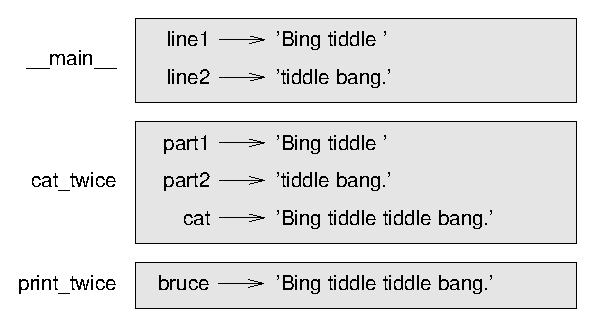
\includegraphics{figs/stack.eps}}
\afterfig

The frames are arranged in a stack that indicates which function
called which, and so on.  In this example, \verb"print_twice"
was called by \verb"cat_twice", and \verb"cat_twice" was called by 
\verb"__main__", which is a special name for the topmost frame.  When
you create a variable outside of any function, it belongs to 
\verb"__main__".

Each parameter refers to the same value as its corresponding
argument.  So, {\tt part1} has the same value as
{\tt line1}, {\tt part2} has the same value as {\tt line2},
and {\tt bruce} has the same value as {\tt cat}.

If an error occurs during a function call, Python prints the
name of the function, and the name of the function that called
it, and the name of the function that called {\em that}, all the
way back to \verb"__main__".

For example, if you try to access {\tt cat} from within 
\verb"print_twice", you get a {\tt NameError}:

\beforeverb
\begin{verbatim}
Traceback (innermost last):
  File "test.py", line 13, in __main__
    cat_twice(line1, line2)
  File "test.py", line 5, in cat_twice
    print_twice(cat)
  File "test.py", line 9, in print_twice
    print cat
NameError: name 'cat' is not defined
\end{verbatim}
\afterverb
%
This list of functions is called a {\bf traceback}.  It tells you what
program file the error occurred in, and what line, and what functions
were executing at the time.  It also shows the line of code that
caused the error.

\index{traceback}

The order of the functions in the traceback is the same as the
order of the frames in the stack diagram.  The function that is
currently running is at the bottom.


\section{Boolean functions}
\label{boolean}

\index{boolean function}

Functions can return booleans, which is often convenient for hiding
complicated tests inside functions.  For example:

\beforeverb
\begin{verbatim}
def is_divisible(x, y):
    if x % y == 0:
        return True
    else:
        return False
\end{verbatim}
\afterverb
%
It is common to give boolean functions names that sound like yes/no
questions; \verb"is_divisible" returns either {\tt True} or {\tt False}
to indicate whether {\tt x} is divisible by {\tt y}.

Here is an example:

\beforeverb
\begin{verbatim}
>>>   is_divisible(6, 4)
False
>>>   is_divisible(6, 3)
True
\end{verbatim}
\afterverb
%
The result of the {\tt ==} operator is a boolean, so we can write the
function more concisely by returning it directly:

\beforeverb
\begin{verbatim}
def is_divisible(x, y):
    return x % y == 0
\end{verbatim}
\afterverb
%
Boolean functions are often used in conditional statements:

\index{conditional statement}
\index{statement!conditional}

\beforeverb
\begin{verbatim}
if is_divisible(x, y):
    print 'x is divisible by y'
\end{verbatim}
\afterverb
%
It might be tempting to write something like:

\beforeverb
\begin{verbatim}
if is_divisible(x, y) == True:
    print 'x is divisible by y'
\end{verbatim}
\afterverb
%
But the extra comparison is unnecessary.

\begin{ex}
Write a function \verb"is_between(x, y, z)" that
returns {\tt True} if $x \le y \le z$ or {\tt False} otherwise.
\end{ex}

\section{Optional parameters}

\index{optional parameter}
\index{parameter!optional}

We have seen built-in functions and methods that take a variable
number of arguments.  It is possible to write user-defined functions
with optional arguments, too.  For example, here is a function that
prints the most common words in a histogram

\beforeverb
\begin{verbatim}
def print_most_common(hist, num=10)
    t = most_common(hist)
    print 'The most common words are:'
    for freq, word in t[0:num]:
        print word, '\t', freq
\end{verbatim}
\afterverb

The first parameter is required; the second is optional.
The {\bf default value} of {\tt num} is 10.

\index{default value}
\index{value!default}

If you only provide one argument:

\beforeverb
\begin{verbatim}
print_most_common(hist)
\end{verbatim}
\afterverb

{\tt num} gets the default value.  If you provide two arguments:

\beforeverb
\begin{verbatim}
print_most_common(hist, 20)
\end{verbatim}
\afterverb

{\tt num} gets the value of the argument instead.  In other
words, the optional argument {\bf overrides} the default value.

\index{override}

If a function has both required and optional parameters, all
the required parameters have to come first, followed by the
optional ones.

% TBD - May want to talk about "guarding" code here - lots removed

\section{Debugging}
\label{factdebug}

\index{debugging}

Breaking a large program into smaller functions creates natural
checkpoints for debugging.  If a function is not working, there are
three possibilities to consider:

\begin{itemize}

\item There is something wrong with the arguments the function
is getting; a precondition is violated.

\item There is something wrong with the function; a postcondition
is violated.

\item There is something wrong with the return value or the
way it is being used.

\end{itemize}

To rule out the first possibility, you can add a {\tt print} statement
at the beginning of the function and display the values of the
parameters (and maybe their types).  Or you can write code
that checks the preconditions explicitly.

\index{precondition}
\index{postcondition}

If the parameters look good, add a {\tt print} statement before each
{\tt return} statement that displays the return value.  If
possible, check the result by hand.  Consider calling the
function with values that make it easy to check the result
(as in Section~\ref{incremental development}).

If the function seems to be working, look at the function call
to make sure the return value is being used correctly (or used
at all!).

\index{flow of execution}

Adding print statements at the beginning and end of a function
can help make the flow of execution more visible.

If you are confused about the flow of execution, this kind of
output can be helpful.  It takes some time to develop effective
scaffolding, but a little bit of scaffolding can save a lot of debugging.


\section{Glossary}

\begin{description}

\item[call graph:] A diagram that shows every frame created during
the execution of a program, with an arrow from each caller to
each callee. 

\index{call graph}
\index{diagram!call graph}

\item[dead code:]  Part of a program that can never be executed, often because
it appears after a {\tt return} statement.
\index{dead code}

\item[declaration:] A statement like {\tt global} that tells the
interpreter something about a variable.
\index{declaration}

\item[default value:] The value given to an optional parameter if no
argument is provided.
\index{default value}

\item[flag:] A boolean variable used to indicate whether a condition
is true.
\index{flag}

\item[frame:]  A box in a stack diagram that represents a function call.
It contains the local variables and parameters of the function.
\index{function frame}
\index{frame}

\item[global variable:]  A variable defined outside a function.  Global
variables can be accessed from any function.
\index{global variable}

\item[guardian:]  A programming pattern that uses a conditional
statement to check for and handle circumstances that
might cause an error.
\index{guardian pattern}
\index{pattern!guardian}

\item[incremental development:]  A program development plan intended to
avoid debugging by adding and testing only
a small amount of code at a time.
\index{incremental development}

\item[local variable:]  A variable defined inside a function.  A local
variable can only be used inside its function.
\index{local variable}

\item[{\tt None}:]  A special value returned by functions that
have no return statement or a return statement without an argument.
\index{None special value}
\index{special value!None}

\item[override:] To replace a default value with an argument.
\index{override}

\item[scaffolding:]  Code that is used during program development but is
not part of the final version.
\index{scaffolding}

\item[stack diagram:]  A graphical representation of a stack of functions,
their variables, and the values they refer to.
\index{stack diagram}

\item[temporary variable:]  A variable used to store an intermediate value in
a complex calculation.
\index{temporary variable}
\index{variable!temporary}

\item[traceback:]  A list of the functions that are executing,
printed when an exception occurs.
\index{traceback}


\end{description}


\section{Exercises}

\begin{ex}
\index{stack diagram}

Draw a stack diagram for the following
program.  What does the program print?

\beforeverb
\begin{verbatim}
def b(z):
    prod = a(z, z)
    print z, prod
    return prod

def a(x, y):
    x = x + 1
    return x * y

def c(x, y, z):
    sum = x + y + z
    pow = b(sum)**2
    return pow

x = 1
y = x + 1
print c(x, y+3, x+y)
\end{verbatim}
\afterverb

\end{ex}



\begin{ex}
\label{palindrome}

\index{palindrome}

A palindrome is a word that is spelled the same backward and
forward, like ``noon'' and ``redivider''.  Recursively, a word
is a palindrome if the first and last letters are the same
and the middle is a palindrome.

The following are functions that take a string argument and
return the first, last, and middle letters:

\beforeverb
\begin{verbatim}
def first(word):
    return word[0]

def last(word):
    return word[-1]

def middle(word):
    return word[1:-1]
\end{verbatim}
\afterverb
%
% TODO: Remove this
We'll see how they work in Chapter~\ref{strings}.

\begin{enumerate}

\item Type these functions into a file named {\tt palindrome.py}
and test them out.  What happens if you call {\tt middle} with
a string with two letters?  One letter?  What about the empty
string, which is written \verb"''" and contains no letters?

\item Write a function called \verb"is_palindrome" that takes
a string argument and returns {\tt True} if it is a palindrome
and {\tt False} otherwise.  Remember that you can use the
built-in function {\tt len} to check the length of a string.

\end{enumerate}

\end{ex}

\begin{ex}
A number, $a$, is a power of $b$ if it is divisible by $b$
and $a/b$ is a power of $b$.  Write a function called
\verb"is_power" that takes parameters {\tt a} and {\tt b}
and returns {\tt True} if {\tt a} is a power of {\tt b}.
\end{ex}


\begin{ex}

\index{greatest common divisor (GCD)}
\index{GCD (greatest common divisor)}

The greatest common divisor (GCD) of $a$ and $b$ is the largest number
that divides both of them with no remainder\footnote{This exercise is
  based on an example from Abelson and Sussman's {\em Structure and
    Interpretation of Computer Programs}.}.

One way to find the GCD of two numbers is Euclid's algorithm,
which is based on the observation that if $r$ is the remainder
when $a$ is divided by $b$, then $gcd(a, b) = gcd(b, r)$.
As a base case, we can consider $gcd(a, 0) = a$.

\index{Euclid's algorithm}
\index{algorithm!Euclid}

Write a function called
\verb"gcd" that takes parameters {\tt a} and {\tt b}
and returns their greatest common divisor.  If you need
help, see \url{wikipedia.org/wiki/Euclidean_algorithm}.

\end{ex}

\chapter{Classes and objects}


\section{User-defined types}
\label{point}

\index{user-defined type}
\index{type!user-defined}

We have used many of Python's built-in types; now we are going
to define a new type.  As an example, we will create a type
called {\tt Point} that represents a point in two-dimensional
space.

\index{point, mathematical}

In mathematical notation, points are often written in
parentheses with a comma separating the coordinates. For example,
$(0, 0)$ represents the origin, and $(x, y)$ represents the
point $x$ units to the right and $y$ units up from the origin.

There are several ways we might represent points in Python:

\begin{itemize}

\item We could store the coordinates separately in two
variables, {\tt x} and {\tt y}.

\item We could store the coordinates as elements in a list
or tuple.

\item We could create a new type to represent points as
objects.

\end{itemize}

\index{representation}

Creating a new type
is (a little) more complicated than the other options, but
it has advantages that will be apparent soon.

A user-defined type is also called a {\bf class}.
A class definition looks like this:

\index{class}
\index{object}
\index{class definition}
\index{definition!class}

\beforeverb
\begin{verbatim}
class Point(object):
    """represents a point in 2-D space"""
\end{verbatim}
\afterverb
%
This header indicates that the new class is a {\tt Point},
which is a kind of {\tt object}, which is a built-in
type.

\index{Point class}
\index{class!Point}

The body is a docstring that explains what the class is for.
You can define variables and functions inside a class definition,
but we will get back to that later.

\index{docstring}

Defining a class named {\tt Point} creates a class object.

\beforeverb
\begin{verbatim}
>>> print Point
<class '__main__.Point'>
\end{verbatim}
\afterverb
%
Because {\tt Point} is defined at the top level, its ``full
name'' is \verb"__main__.Point".

\index{object!class}
\index{class object}

The class object is like a factory for creating objects.  To create a
Point, you call {\tt Point} as if it were a function.

\beforeverb
\begin{verbatim}
>>> blank = Point()
>>> print blank
<__main__.Point instance at 0xb7e9d3ac>
\end{verbatim}
\afterverb
%
The return value is a reference to a Point object, which we
assign to {\tt blank}.  
Creating a new object is called
{\bf instantiation}, and the object is an {\bf instance} of
the class.

\index{instance}
\index{instantiation}

When you print an instance, Python tells you what class it
belongs to and where it is stored in memory (the prefix
{\tt 0x} means that the following number is in hexadecimal).

\index{hexadecimal}


\section{Attributes}

\index{instance attribute}
\index{attribute!instance}
\index{dot notation}

You can assign values to an instance using dot notation:

\beforeverb
\begin{verbatim}
>>> blank.x = 3.0
>>> blank.y = 4.0
\end{verbatim}
\afterverb
%
This syntax is similar to the syntax for selecting a variable from a
module, such as {\tt math.pi} or {\tt string.whitespace}.  In this case,
though, we are assigning values to named elements of an object.
These elements are called {\bf attributes}.

As a noun, ``AT-trib-ute'' is pronounced with emphasis on the first
syllable, as opposed to ``a-TRIB-ute,'' which is a verb.

The following diagram shows the result of these assignments.
A state diagram that shows an object and its attributes is
called an {\bf object diagram}:

\index{state diagram}
\index{diagram!state}
\index{object diagram}
\index{diagram!object}

\beforefig
\centerline{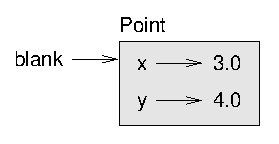
\includegraphics{figs/point.eps}}
\afterfig

The variable {\tt blank} refers to a Point object, which
contains two attributes.  Each attribute refers to a
floating-point number.

You can read the value of an attribute using the same syntax:

\beforeverb
\begin{verbatim}
>>> print blank.y
4.0
>>> x = blank.x
>>> print x
3.0
\end{verbatim}
\afterverb
%
The expression {\tt blank.x} means, ``Go to the object {\tt blank}
refers to and get the value of {\tt x}.'' In this case, we assign that
value to a variable named {\tt x}.  There is no conflict between
the variable {\tt x} and the attribute {\tt x}.

You can use dot notation as part of any expression.  For example:

\beforeverb
\begin{verbatim}
>>> print '(%g, %g)' % (blank.x, blank.y)
(3.0, 4.0)
>>> distance = math.sqrt(blank.x**2 + blank.y**2)
>>> print distance
5.0
\end{verbatim}
\afterverb
%
You can pass an instance as an argument in the usual way.
For example:

\index{instance!as argument}

\beforeverb
\begin{verbatim}
def print_point(p):
    print '(%g, %g)' % (p.x, p.y)
\end{verbatim}
\afterverb
%
\verb"print_point" takes a point as an argument and displays it in
mathematical notation.  To invoke it, you can pass {\tt blank} as
an argument:

\beforeverb
\begin{verbatim}
>>> print_point(blank)
(3.0, 4.0)
\end{verbatim}
\afterverb
%
Inside the function, {\tt p} is an alias for {\tt blank}, so if
the function modifies {\tt p}, {\tt blank} changes.

\index{aliasing}


\begin{ex}
Write a function called {\tt distance} that takes two Points
as arguments and returns the distance between them.
\end{ex}



\section{Rectangles}

Sometimes it is obvious what the attributes of an object should be,
but other times you have to make decisions.  For example, imagine you
are designing a class to represent rectangles.  What attributes would
you use to specify the location and size of a rectangle?  You can
ignore angle; to keep things simple, assume that the rectangle is
either vertical or horizontal.

\index{representation}

There are at least two possibilities: 

\begin{itemize}

\item You could specify one corner of the rectangle
(or the center), the width, and the height.

\item You could specify two opposing corners.

\end{itemize}

At this point it is hard to say whether either is better than
the other, so we'll implement the first one, just as an example.

\index{Rectangle class}
\index{class!Rectangle}

Here is the class definition:

\beforeverb
\begin{verbatim}
class Rectangle(object):
    """represent a rectangle. 
       attributes: width, height, corner.
    """
\end{verbatim}
\afterverb
%
The docstring lists the attributes:  {\tt width} and
{\tt height} are numbers; {\tt corner} is a Point object that
specifies the lower-left corner.

To represent a rectangle, you have to instantiate a Rectangle
object and assign values to the attributes:

\beforeverb
\begin{verbatim}
box = Rectangle()
box.width = 100.0
box.height = 200.0
box.corner = Point()
box.corner.x = 0.0
box.corner.y = 0.0
\end{verbatim}
\afterverb
%
The expression {\tt box.corner.x} means,
``Go to the object {\tt box} refers to and select the attribute named
{\tt corner}; then go to that object and select the attribute named
{\tt x}.''

The figure shows the state of this object:

\index{state diagram}
\index{diagram!state}
\index{object diagram}
\index{diagram!object}

\beforefig
\centerline{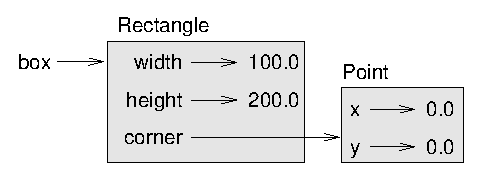
\includegraphics{figs/rectangle.eps}}
\afterfig

An object that is an attribute of another object is {\bf embedded}.

\index{embedded object}
\index{object!embedded}


\section{Instances as return values}

\index{instance!as return value}
\index{return value}

Functions can return instances.  For example, \verb"find_center"
takes a {\tt Rectangle} as an argument and returns a {\tt Point}
that contains the coordinates of the center of the {\tt Rectangle}:

\beforeverb
\begin{verbatim}
def find_center(box):
    p = Point()
    p.x = box.corner.x + box.width/2.0
    p.y = box.corner.y + box.height/2.0
    return p
\end{verbatim}
\afterverb
%
Here is an example that passes {\tt box} as an argument and assigns
the resulting Point to {\tt center}:

\beforeverb
\begin{verbatim}
>>> center = find_center(box)
>>> print_point(center)
(50.0, 100.0)
\end{verbatim}
\afterverb
%

\section{Objects are mutable}

\index{object!mutable}
\index{mutability}

You can change the state of an object by making an assignment to one of
its attributes.  For example, to change the size of a rectangle
without changing its position, you can modify the values of {\tt
width} and {\tt height}:

\beforeverb
\begin{verbatim}
box.width = box.width + 50
box.height = box.width + 100
\end{verbatim}
\afterverb
%
You can also write functions that modify objects.  For example,
\verb"grow_rectangle" takes a Rectangle object and two numbers,
{\tt dwidth} and {\tt dheight}, and adds the numbers to the
width and height of the rectangle:

\beforeverb
\begin{verbatim}
def grow_rectangle(rect, dwidth, dheight) :
    rect.width += dwidth
    rect.height += dheight
\end{verbatim}
\afterverb
%
Here is an example that demonstrates the effect:

\beforeverb
\begin{verbatim}
>>> print box.width
100.0
>>> print box.height
200.0
>>> grow_rectangle(box, 50, 100)
>>> print box.width
150.0
>>> print box.height
300.0
\end{verbatim}
\afterverb
%
Inside the function, {\tt rect} is an
alias for {\tt box}, so if the function modifies {\tt rect}, 
{\tt box} changes.

\begin{ex}
Write a function named \verb"move_rectangle" that takes
a Rectangle and two numbers named {\tt dx} and {\tt dy}.  It
should change the location of the rectangle by adding {\tt dx}
to the {\tt x} coordinate of {\tt corner} and adding {\tt dy}
to the {\tt y} coordinate of {\tt corner}.
\end{ex}


\section{Copying}

\index{aliasing}

Aliasing can make a program difficult to read because changes
in one place might have unexpected effects in another place.
It is hard to keep track of all the variables that might refer
to a given object.

\index{copying objects}
\index{object!copying}
\index{copy module}
\index{module!copy}

Copying an object is often an alternative to aliasing.
The {\tt copy} module contains a function called {\tt copy} that
can duplicate any object:

\beforeverb
\begin{verbatim}
>>> p1 = Point()
>>> p1.x = 3.0
>>> p1.y = 4.0

>>> import copy
>>> p2 = copy.copy(p1)
\end{verbatim}
\afterverb
%
{\tt p1} and {\tt p2} contain the same data, but they are
not the same Point.

\beforeverb
\begin{verbatim}
>>> print_point(p1)
(3.0, 4.0)
>>> print_point(p2)
(3.0, 4.0)
>>> p1 is p2
False
>>> p1 == p2
False
\end{verbatim}
\afterverb
%
The {\tt is} operator indicates that {\tt p1} and {\tt p2} are not the
same object, which is what we expected.  But you might have expected
{\tt ==} to yield {\tt True} because these points contain the same
data.  In that case, you will be disappointed to learn that for
instances, the default behavior of the {\tt ==} operator is the same
as the {\tt is} operator; it checks object identity, not object
equivalence.  This behavior can be changed---we'll see how later.

\index{is operator}
\index{operator!is}

If you use {\tt copy.copy} to duplicate a Rectangle, you will find
that it copies the Rectangle object but not the embedded Point.

\index{embedded object!copying}

\beforeverb
\begin{verbatim}
>>> box2 = copy.copy(box)
>>> box2 is box
False
>>> box2.corner is box.corner
True
\end{verbatim}
\afterverb
%
Here is what the object diagram looks like:

\index{state diagram}
\index{diagram!state}
\index{object diagram}
\index{diagram!object}

\vspace{0.1in}
\beforefig
\centerline{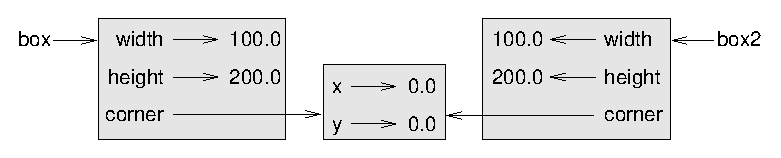
\includegraphics{figs/rectangle2.eps}}
\afterfig
\vspace{0.1in}

This operation is called a {\bf shallow copy} because it copies the
object and any references it contains, but not the embedded objects.

\index{shallow copy}
\index{copy!shallow}

For most applications, this is not what you want.  In this example,
invoking \verb"grow_rectangle" on one of the Rectangles would not
affect the other, but invoking \verb"move_rectangle" on either would
affect both!  This behavior is confusing and error-prone.

\index{deep copy}
\index{copy!deep}

Fortunately, the {\tt copy} module contains a method named {\tt
deepcopy} that copies not only the object but also 
the objects it refers to, and the objects {\em they} refer to,
and so on.
You will not be surprised to learn that this operation is
called a {\bf deep copy}.

\index{deepcopy function}
\index{function!deepcopy}

\beforeverb
\begin{verbatim}
>>> box3 = copy.deepcopy(box)
>>> box3 is box
False
>>> box3.corner is box.corner
False
\end{verbatim}
\afterverb
%
{\tt box3} and {\tt box} are completely separate objects.


\begin{ex}
Write a version of \verb"move_rectangle" that creates and
returns a new Rectangle instead of modifying the old one.
\end{ex}


\section{Debugging}
\label{hasattr}

\index{debugging}

When you start working with objects, you are likely to encounter
some new exceptions.  If you try to access an attribute
that doesn't exist, you get an {\tt AttributeError}:

\index{exception!AttributeError}
\index{AttributeError}

\beforeverb
\begin{verbatim}
>>> p = Point()
>>> print p.z
AttributeError: Point instance has no attribute 'z'
\end{verbatim}
\afterverb
%
If you are not sure what type an object is, you can ask:

\index{type function}
\index{function!type}

\beforeverb
\begin{verbatim}
>>> type(p)
<type '__main__.Point'>
\end{verbatim}
\afterverb
%
If you are not sure whether an object has a particular attribute,
you can use the built-in function {\tt hasattr}:

\index{hasattr function}
\index{function!hasattr}

\beforeverb
\begin{verbatim}
>>> hasattr(p, 'x')
True
>>> hasattr(p, 'z')
False
\end{verbatim}
\afterverb
%
The first argument can be any object; the second argument is a {\em
string} that contains the name of the attribute.


\section{Glossary}

\begin{description}

\item[class:] A user-defined type.  A class definition creates a new
class object.
\index{class}

\item[class object:] An object that contains information about a
user-defined type.  The class object can be used to create instances
of the type.
\index{class object}

\item[instance:] An object that belongs to a class.
\index{instance}

\item[attribute:] One of the named values associated with an object.
\index{attribute!instance}
\index{instance attribute}

\item[embedded (object):] An object that is stored as an attribute
of another object.
\index{embedded object}
\index{object!embedded}

\item[shallow copy:] To copy the contents of an object, including
any references to embedded objects;
implemented by the {\tt copy} function in the {\tt copy} module.
\index{shallow copy}

\item[deep copy:] To copy the contents of an object as well as any
embedded objects, and any objects embedded in them, and so on;
implemented by the {\tt deepcopy} function in the {\tt copy} module.
\index{deep copy}

\item[object diagram:] A diagram that shows objects, their
attributes, and the values of the attributes.
\index{object diagram}
\index{diagram!object}

\end{description}


\chapter{Classes and functions}
\label{time}


\section{Time}

As another example of a user-defined type, we'll define a class called
{\tt Time} that records the time of day.  The class definition looks
like this:

\index{user-defined type}
\index{type!user-defined}
\index{Time class}
\index{class!Time}

\beforeverb
\begin{verbatim}
class Time(object):
    """represents the time of day.
       attributes: hour, minute, second"""
\end{verbatim}
\afterverb
%
We can create a new {\tt Time} object and assign
attributes for hours, minutes, and seconds:

\beforeverb
\begin{verbatim}
time = Time()
time.hour = 11
time.minute = 59
time.second = 30
\end{verbatim}
\afterverb
%
The state diagram for the {\tt Time} object looks like this:

\index{state diagram}
\index{diagram!state}
\index{object diagram}
\index{diagram!object}

\beforefig
\centerline{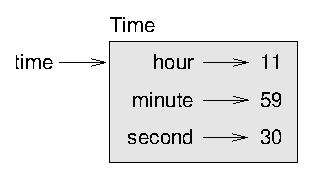
\includegraphics{figs/time.eps}}
\afterfig

\begin{ex}
\label{printtime}
Write a function called \verb"print_time" that takes a 
Time object and prints it in the form {\tt hour:minute:second}.
Hint: the format sequence \verb"'%.2d'" prints an integer using
at least two digits, including a leading zero if necessary.
\end{ex}

\begin{ex}
\label{is_after}

\index{boolean function}

Write a boolean function called \verb"is_after" that
takes two Time objects, {\tt t1} and {\tt t2}, and
returns {\tt True} if {\tt t1} follows {\tt t2} chronologically and
{\tt False} otherwise.  Challenge: don't use an {\tt if} statement.
\end{ex}


\section{Pure functions}

\index{prototype and patch}
\index{development plan!prototype and patch}

In the next few sections, we'll write two functions that add time
values.  They demonstrate two kinds of functions: pure functions and
modifiers.  They also demonstrate a development plan I'll call {\bf
  prototype and patch}, which is a way of tackling a complex problem
by starting with a simple prototype and incrementally dealing with the
complications.

Here is a simple prototype of \verb"add_time":

\beforeverb
\begin{verbatim}
def add_time(t1, t2):
    sum = Time()
    sum.hour = t1.hour + t2.hour
    sum.minute = t1.minute + t2.minute
    sum.second = t1.second + t2.second
    return sum
\end{verbatim}
\afterverb
%
The function creates a new {\tt Time} object, initializes its
attributes, and returns a reference to the new object.  This is called
a {\bf pure function} because it does not modify any of the objects
passed to it as arguments and it has no effect,
like displaying a value or getting user input, 
other than returning a value.

\index{pure function}
\index{function type!pure}

To test this function, I'll create two Time objects: {\tt start}
contains the start time of a movie, like {\em Monty Python and the
Holy Grail}, and {\tt duration} contains the run time of the movie,
which is one hour 35 minutes.

\index{Monty Python and the Holy Grail}

\verb"add_time" figures out when the movie will be done.

\beforeverb
\begin{verbatim}
>>> start = Time()
>>> start.hour = 9
>>> start.minute = 45
>>> start.second =  0

>>> duration = Time()
>>> duration.hour = 1
>>> duration.minute = 35
>>> duration.second = 0

>>> done = add_time(start, duration)
>>> print_time(done)
10:80:00
\end{verbatim}
\afterverb
%
The result, {\tt 10:80:00} might not be what you were hoping
for.  The problem is that this function does not deal with cases where the
number of seconds or minutes adds up to more than sixty.  When that
happens, we have to ``carry'' the extra seconds into the minute column
or the extra minutes into the hour column.

\index{carrying, addition with}

Here's an improved version:

\beforeverb
\begin{verbatim}
def add_time(t1, t2):
    sum = Time()
    sum.hour = t1.hour + t2.hour
    sum.minute = t1.minute + t2.minute
    sum.second = t1.second + t2.second

    if sum.second >= 60:
        sum.second -= 60
        sum.minute += 1

    if sum.minute >= 60:
        sum.minute -= 60
        sum.hour += 1

    return sum
\end{verbatim}
\afterverb
%
Although this function is correct, it is starting to get big.
We will see a shorter alternative later.


\section{Modifiers}
\label{increment}

\index{modifier}
\index{function type!modifier}

Sometimes it is useful for a function to modify the objects it gets as
parameters.  In that case, the changes are visible to the caller.
Functions that work this way are called {\bf modifiers}.

\index{increment}

{\tt increment}, which adds a given number of seconds to a {\tt Time}
object, can be written naturally as a
modifier.  Here is a rough draft:

\beforeverb
\begin{verbatim}
def increment(time, seconds):
    time.second += seconds

    if time.second >= 60:
        time.second -= 60
        time.minute += 1

    if time.minute >= 60:
        time.minute -= 60
        time.hour += 1
\end{verbatim}
\afterverb
%
The first line performs the basic operation; the remainder deals
with the special cases we saw before.

\index{special case}

Is this function correct?  What happens if the parameter {\tt seconds}
is much greater than sixty?  

In that case, it is not enough to carry
once; we have to keep doing it until {\tt time.second} is less than sixty.
One solution is to replace the {\tt if} statements with {\tt while}
statements.  That would make the function correct, but not
very efficient.

\begin{ex}
Write a correct version of {\tt increment} that
doesn't contain any loops.
\end{ex}

Anything that can be done with modifiers can also be done with pure
functions.  In fact, some programming languages only allow pure
functions.  There is some evidence that programs that use pure
functions are faster to develop and less error-prone than programs
that use modifiers.  But modifiers are convenient at times,
and functional programs tend to be less efficient.

In general, I recommend that you write pure functions whenever it is
reasonable and resort to modifiers only if there is a compelling
advantage.  This approach might be called a {\bf functional
programming style}.

\index{functional programming style}


\begin{ex}
Write a ``pure'' version of {\tt increment} that creates and returns
a new Time object rather than modifying the parameter.
\end{ex}


\section{Prototyping versus planning}
\label{prototype}

\index{prototype and patch}
\index{development plan!prototype and patch}
\index{planned development}
\index{development plan!planned}

The development plan I am demonstrating is called ``prototype and
patch.''  For each function, I wrote a prototype that performed the
basic calculation and then tested it, patching errors along the
way.

This approach can be effective, especially if you don't yet have a
deep understanding of the problem.  But incremental corrections can
generate code that is unnecessarily complicated---since it deals with
many special cases---and unreliable---since it is hard to know if you
have found all the errors.

An alternative is {\bf planned development}, in which high-level
insight into the problem can make the programming much easier.  In
this case, the insight is that a Time object is really a three-digit
number in base 60 (see \url{wikipedia.org/wiki/Sexagesimal})!  The
{\tt second} attribute is the ``ones column,'' the {\tt minute}
attribute is the ``sixties column,'' and the {\tt hour} attribute is
the ``thirty-six hundreds column.''

\index{sexagesimal}

When we wrote \verb"add_time" and {\tt increment}, we were effectively
doing addition in base 60, which is why we had to carry from one
column to the next.

\index{carrying, addition with}

This observation suggests another approach to the whole problem---we
can convert Time objects to integers and take advantage of the fact
that the computer knows how to do integer arithmetic.  

Here is a function that converts Times to integers:

\beforeverb
\begin{verbatim}
def time_to_int(time):
    minutes = time.hour * 60 + time.minute
    seconds = minutes * 60 + time.second
    return seconds
\end{verbatim}
\afterverb
%
And here is the function that converts integers to Times
(recall that {\tt divmod} divides the first argument by the second
and returns the quotient and remainder as a tuple).

\index{divmod}

\beforeverb
\begin{verbatim}
def int_to_time(seconds):
    time = Time()
    minutes, time.second = divmod(seconds, 60)
    time.hour, time.minute = divmod(minutes, 60)
    return time
\end{verbatim}
\afterverb
%
You might have to think a bit, and run some tests, to convince
yourself that these functions are correct.  One way to test them is to
check that \verb"time_to_int(int_to_time(x)) == x" for many values of
{\tt x}.  This is an example of a consistency check.

\index{consistency check}

Once you are convinced they are correct, you can use them to 
rewrite \verb"add_time":

\beforeverb
\begin{verbatim}
def add_time(t1, t2):
    seconds = time_to_int(t1) + time_to_int(t2)
    return int_to_time(seconds)
\end{verbatim}
\afterverb
%
This version is shorter than the original, and easier to verify.

\begin{ex}
Rewrite {\tt increment} using \verb"time_to_int" and \verb"int_to_time".
\end{ex}

In some ways, converting from base 60 to base 10 and back is harder
than just dealing with times.  Base conversion is more abstract; our
intuition for dealing with time values is better.

But if we have the insight to treat times as base 60 numbers and make
the investment of writing the conversion functions (\verb"time_to_int"
and \verb"int_to_time"), we get a program that is shorter, easier to
read and debug, and more reliable.

It is also easier to add features later.  For example, imagine
subtracting two Times to find the duration between them.  The
na\"{\i}ve approach would be to implement subtraction with borrowing.
Using the conversion functions would be easier and more likely to be
correct.

\index{subtraction with borrowing}
\index{borrowing, subtraction with}
\index{generalization}

Ironically, sometimes making a problem harder (or more general) makes it
easier (because there are fewer special cases and fewer opportunities
for error).


\section{Debugging}
\index{debugging}

A Time object is well-formed if the values of {\tt minutes} and {\tt
seconds} are between 0 and 60 (including 0 but not 60) and if 
{\tt hours} is positive.  {\tt hours} and {\tt minutes} should be
integral values, but we might allow {\tt seconds} to have a
fraction part.

\index{invariant}

These kind of requirements are called {\bf invariants} because
they should always be true.  To put it a different way, if they
are not true, then something has gone wrong.

Writing code to check your invariants can help you detect errors
and find their causes.  For example, you might have a function
like \verb"valid_time" that takes a Time object and returns
{\tt False} if it violates an invariant:

\beforeverb
\begin{verbatim}
def valid_time(time):
    if time.hours < 0 or time.minutes < 0 or time.seconds < 0:
        return False
    if time.minutes >= 60 or time.seconds >= 60:
        return False
    return True
\end{verbatim}
\afterverb
%
Then at the beginning of each function you could check the
arguments to make sure they are valid:

\index{raise statement}
\index{statement!raise}

\beforeverb
\begin{verbatim}
def add_time(t1, t2):
    if not valid_time(t1) or not valid_time(t2):
        raise ValueError, 'invalid Time object in add_time'
    seconds = time_to_int(t1) + time_to_int(t2)
    return int_to_time(seconds)
\end{verbatim}
\afterverb
%
Or you could use an {\tt assert} statement, which checks a given invariant
and raises an exception if it fails:

\index{assert statement}
\index{statement!assert}

\beforeverb
\begin{verbatim}
def add_time(t1, t2):
    assert valid_time(t1) and valid_time(t2)
    seconds = time_to_int(t1) + time_to_int(t2)
    return int_to_time(seconds)
\end{verbatim}
\afterverb
%
{\tt assert} statements are useful because they distinguish
code that deals with normal conditions from code
that checks for errors.


\section{Glossary}

\begin{description}

\item[prototype and patch:] A development plan that involves
writing a rough draft of a program, testing, and correcting errors as
they are found.
\index{prototype and patch}

\item[planned development:] A development plan that involves
high-level insight into the problem and more planning than incremental
development or prototype development.
\index{planned development}

\item[pure function:] A function that does not modify any of the objects it
receives as arguments.  Most pure functions are fruitful.
\index{pure function}

\item[modifier:] A function that changes one or more of the objects it
receives as arguments.  Most modifiers are fruitless.
\index{modifier}

\item[functional programming style:] A style of program design in which the
majority of functions are pure.
\index{functional programming style}

\item[invariant:] A condition that should always be true during the
execution of a program.
\index{invariant}

\end{description}


\section{Exercises}

\begin{ex}
Write a function called \verb"mul_time" that takes a Time object
and a number and returns a new Time object that contains
the product of the original Time and the number.

Then use \verb"mul_time" to write a function that takes a Time
object that represents the finishing time in a race, and a number
that represents the distance, and returns a Time object that represents
the average pace (time per mile).

\index{running pace}

\end{ex}

\begin{ex}

\index{Date class}
\index{class!Date}

Write a class definition for a Date object that has attributes {\tt
  day}, {\tt month} and {\tt year}.  Write a function called
\verb"increment_date" that takes a Date object, {\tt date} and an
integer, {\tt n}, and returns a new Date object that
represents the day {\tt n} days after {\tt date}.  Hint:
``Thirty days hath September...''  Challenge: does your function
deal with leap years correctly?  See \url{wikipedia.org/wiki/Leap_year}

\end{ex}


\begin{ex}

\index{datetime module}
\index{module!datetime}

The {\tt datetime} module provides {\tt date} and {\tt time} objects
that are similar to the Date and Time objects in this chapter, but
they provide a rich set of methods and operators.  Read the
documentation at \url{docs.python.org/lib/datetime-date.html}.

\begin{enumerate}

\item Use the {\tt datetime} module to write a program that
gets the current date and prints the day of the week.

\index{birthday}

\item Write a program that takes a birthday as input
and prints the user's age and the number of days, hours,
minutes and seconds until their next birthday.
\end{enumerate}

\end{ex}


\chapter{Classes and methods}


\section{Object-oriented features}

\index{object-oriented programming}

Python is an {\bf object-oriented programming language}, which means
that it provides features that support object-oriented
programming.

It is not easy to define object-oriented programming, but we have
already seen some of its characteristics:

\begin{itemize}

\item Programs are made up of object definitions and function
definitions, and most of the computation is expressed in terms
of operations on objects.

\item Each object definition corresponds to some object or concept
in the real world, and the functions that operate on that object
correspond to the ways real-world objects interact.

\end{itemize}

For example, the {\tt Time} class defined in Chapter~\ref{time}
corresponds to the way people record the time of day, and the
functions we defined correspond to the kinds of things people do with
times.  Similarly, the {\tt Point} and {\tt Rectangle} classes
correspond to the mathematical concepts of a point and a rectangle.

So far, we have not taken advantage of the features Python provides to
support object-oriented programming.  These
features are not strictly necessary; most of them provide
alternative syntax for things we have already done.  But in many cases,
the alternative is more concise and more accurately conveys the
structure of the program.

For example, in the {\tt Time} program, there is no obvious
connection between the class definition and the function definitions
that follow.  With some examination, it is apparent that every function
takes at least one {\tt Time} object as an argument.

\index{method}
\index{function}

This observation is the motivation for {\bf methods}; a method is
a function that is associated with a particular class.
We have seen methods for strings, lists, dictionaries and tuples.
In this chapter, we will define methods for user-defined types.

\index{syntax}
\index{semantics}

Methods are semantically the same as functions, but there are
two syntactic differences:

\begin{itemize}

\item Methods are defined inside a class definition in order
to make the relationship between the class and the method explicit.

\item The syntax for invoking a method is different from the
syntax for calling a function.

\end{itemize}

In the next few sections, we will take the functions from the previous
two chapters and transform them into methods.  This transformation is
purely mechanical; you can do it simply by following a sequence of
steps.  If you are comfortable converting from one form to another,
you will be able to choose the best form for whatever you are doing.


\section{Printing objects}
\label{print_time}

\index{object!printing}

In Chapter~\ref{time}, we defined a class named
{\tt Time} and in Exercise~\ref{printtime}, you 
wrote a function named \verb"print_time":

\beforeverb
\begin{verbatim}
class Time(object):
    """represents the time of day.
       attributes: hour, minute, second"""

def print_time(time):
    print '%.2d:%.2d:%.2d' % (time.hour, time.minute, time.second)
\end{verbatim}
\afterverb
%
To call this function, you have to pass a {\tt Time} object as an
argument:

\beforeverb
\begin{verbatim}
>>> start = Time()
>>> start.hour = 9
>>> start.minute = 45
>>> start.second = 00
>>> print_time(start)
09:45:00
\end{verbatim}
\afterverb
%
To make \verb"print_time" a method, all we have to do is
move the function definition inside the class definition.  Notice
the change in indentation.

\index{indentation}

\beforeverb
\begin{verbatim}
class Time(object):
    def print_time(time):
        print '%.2d:%.2d:%.2d' % (time.hour, time.minute, time.second)
\end{verbatim}
\afterverb
%
Now there are two ways to call \verb"print_time".  The first
(and less common) way is to use function syntax:

\index{function syntax}
\index{dot notation}


\beforeverb
\begin{verbatim}
>>> Time.print_time(start)
09:45:00
\end{verbatim}
\afterverb
%
In this use of dot notation, {\tt Time} is the name of the class,
and \verb"print_time" is the name of the method.  {\tt start} is
passed as a parameter.

The second (and more concise) way is to use method syntax:

\index{method syntax}

\beforeverb
\begin{verbatim}
>>> start.print_time()
09:45:00
\end{verbatim}
\afterverb
%
In this use of dot notation, \verb"print_time" is the name of the
method (again), and {\tt start} is the object the method is
invoked on, which is called the {\bf subject}.  Just as the
subject of a sentence is what the sentence is about, the subject
of a method invocation is what the method is about.

\index{subject}

Inside the method, the subject is assigned to the first
parameter, so in this case {\tt start} is assigned
to {\tt time}.

\index{self (parameter name)}
\index{parameter!self}

By convention, the first parameter of a method is
called {\tt self}, so it would be more common to write
\verb"print_time" like this:

\beforeverb
\begin{verbatim}
class Time(object):
    def print_time(self):
        print '%.2d:%.2d:%.2d' % (self.hour, self.minute, self.second)
\end{verbatim}
\afterverb
%
The reason for this convention is an implicit metaphor:

\index{metaphor, method invocation}

\begin{itemize}

\item The syntax for a function call, \verb"print_time(start)",
  suggests that the function is the active agent.  It says something
  like, ``Hey \verb"print_time"!  Here's an object for you to print.''

\item In object-oriented programming, the objects are the active
  agents.  A method invocation like \verb"start.print_time()" says
  ``Hey {\tt start}!  Please print yourself.''

\end{itemize}

This change in perspective might be more polite, but it is not obvious
that it is useful.  In the examples we have seen so far, it may not
be.  But sometimes shifting responsibility from the functions onto the
objects makes it possible to write more versatile functions, and makes
it easier to maintain and reuse code.

\begin{ex}
\label{convert}
Rewrite \verb"time_to_int"
(from Section~\ref{prototype}) as a method.  It is probably not
appropriate to rewrite \verb"int_to_time" as a method; it's not
clear what object you would invoke it on!
\end{ex}


\section{Another example}

\index{increment}

Here's a version of {\tt increment} (from Section~\ref{increment})
rewritten as a method:

\beforeverb
\begin{verbatim}
# inside class Time:

    def increment(self, seconds):
        seconds += self.time_to_int()
        return int_to_time(seconds)
\end{verbatim}
\afterverb
%
This version assumes that \verb"time_to_int" is written
as a method, as in Exercise~\ref{convert}.  Also, note that
it is a pure function, not a modifier.

Here's how you would invoke {\tt increment}:

\beforeverb
\begin{verbatim}
>>> start.print_time()
09:45:00
>>> end = start.increment(1337)
>>> end.print_time()
10:07:17
\end{verbatim}
\afterverb
%
The subject, {\tt start}, gets assigned to the first parameter,
{\tt self}.  The argument, {\tt 1337}, gets assigned to the
second parameter, {\tt seconds}.

This mechanism can be confusing, especially if you make an error.
For example, if you invoke {\tt increment} with two arguments, you
get:

\index{exception!TypeError}
\index{TypeError}

\beforeverb
\begin{verbatim}
>>> end = start.increment(1337, 460)
TypeError: increment() takes exactly 2 arguments (3 given)
\end{verbatim}
\afterverb
%
The error message is initially confusing, because there are
only two arguments in parentheses.  But the subject is also
considered an argument, so all together that's three.


\section{A more complicated example}

\verb"is_after" (from Exercise~\ref{is_after}) is slightly more complicated
because it takes two Time objects as parameters.  In this case it is
conventional to name the first parameter {\tt self} and the second
parameter {\tt other}:

\index{other (parameter name)}
\index{parameter!other}

\beforeverb
\begin{verbatim}
# inside class Time:

    def is_after(self, other):
        return self.time_to_int() > other.time_to_int()
\end{verbatim}
\afterverb
%
To use this method, you have to invoke it on one object and pass
the other as an argument:

\beforeverb
\begin{verbatim}
>>> end.is_after(start)
True
\end{verbatim}
\afterverb
%
One nice thing about this syntax is that it almost reads
like English: ``end is after start?''


\section{The init method}

\index{init method}
\index{method!init}

The init method (short for ``initialization'') is
a special method that gets invoked when an object is instantiated.  
Its full name is \verb"__init__" (two underscore characters,
followed by {\tt init}, and then two more underscores).  An
init method for the {\tt Time} class might look like this:

\beforeverb
\begin{verbatim}
# inside class Time:

    def __init__(self, hour=0, minute=0, second=0):
        self.hour = hour
        self.minute = minute
        self.second = second
\end{verbatim}
\afterverb
%
It is common for the parameters of \verb"__init__"
to have the same names as the attributes.  The statement

\beforeverb
\begin{verbatim}
        self.hour = hour
\end{verbatim}
\afterverb
%
stores the value of the parameter {\tt hour} as an attribute
of {\tt self}.

\index{optional parameter}
\index{parameter!optional}
\index{default value}
\index{override}

The parameters are optional, so if you call {\tt Time} with
no arguments, you get the default values.

\beforeverb
\begin{verbatim}
>>> time = Time()
>>> time.print_time()
00:00:00
\end{verbatim}
\afterverb
%
If you provide one argument, it overrides {\tt hour}:

\beforeverb
\begin{verbatim}
>>> time = Time (9)
>>> time.print_time()
09:00:00
\end{verbatim}
\afterverb
%
If you provide two arguments, they override {\tt hour} and
{\tt minute}.

\beforeverb
\begin{verbatim}
>>> time = Time(9, 45)
>>> time.print_time()
09:45:00
\end{verbatim}
\afterverb
%
And if you provide three arguments, they override all three
default values.


\begin{ex}
\index{Point class}
\index{class!Point}

Write an init method for the {\tt Point} class that takes
{\tt x} and {\tt y} as optional parameters and assigns
them to the corresponding attributes.
\end{ex}


\section{The {\tt \_\_str\_\_} method}

\index{str method@\_\_str\_\_ method}
\index{method!\_\_str\_\_}

\verb"__str__" is a special method, like \verb"__init__",
that is supposed to return a string representation of an object.

\index{string representation}

For example, here is a {\tt str} method for Time objects:

\beforeverb
\begin{verbatim}
# inside class Time:

    def __str__(self):
        return '%.2d:%.2d:%.2d' % (self.hour, self.minute, self.second)
\end{verbatim}
\afterverb
%
When you {\tt print} an object, Python invokes the {\tt str} method:

\index{print statement}
\index{statement!print}

\beforeverb
\begin{verbatim}
>>> time = Time(9, 45)
>>> print time
09:45:00
\end{verbatim}
\afterverb
%
When I write a new class, I almost always start by writing 
\verb"__init__", which makes it easier to instantiate objects, and 
\verb"__str__", which is useful for debugging.


\begin{ex}
Write a {\tt str} method for the {\tt Point} class.  Create
a Point object and print it.
\end{ex}


\section{Operator overloading}
\label{operator overloading}

By defining other special methods, you can specify the behavior
of operators on user-defined types.  For example, if you define
a method named \verb"__add__" for the {\tt Time} class, you can use the
{\tt +} operator on Time objects.

Here is what the definition might look like:

\index{add method}
\index{method!add}

\beforeverb
\begin{verbatim}
# inside class Time:

    def __add__(self, other):
        seconds = self.time_to_int() + other.time_to_int()
        return int_to_time(seconds)
\end{verbatim}
\afterverb
%
And here is how you could use it:

\beforeverb
\begin{verbatim}
>>> start = Time(9, 45)
>>> duration = Time(1, 35)
>>> print start + duration
11:20:00
\end{verbatim}
\afterverb
%
When you apply the {\tt +} operator to Time objects, Python invokes
\verb"__add__".  When you print the result, Python invokes 
\verb"__str__".  So there is quite a lot happening behind the scenes!

\index{operator overloading}

Changing the behavior of an operator so that it works with
user-defined types is called {\bf operator overloading}.  For every
operator in Python there is a corresponding special method, like 
\verb"__add__".  For more details, see
\url{docs.python.org/ref/specialnames.html}.

\begin{ex}
Write an {\tt add} method for the Point class.  
\end{ex}


\section{Type-based dispatch}

In the previous section we added two Time objects, but you
also might want to add an integer to a Time object.  The
following is a version of \verb"__add__"
that checks the type of {\tt other} and invokes either
\verb"add_time" or {\tt increment}:

\beforeverb
\begin{verbatim}
# inside class Time:

    def __add__(self, other):
        if isinstance(other, Time):
            return self.add_time(other)
        else:
            return self.increment(other)

    def add_time(self, other):
        seconds = self.time_to_int() + other.time_to_int()
        return int_to_time(seconds)

    def increment(self, seconds):
        seconds += self.time_to_int()
        return int_to_time(seconds)
\end{verbatim}
\afterverb
%
The built-in function {\tt isinstance} takes a value and a
class object, and returns {\tt True} if the value is an instance
of the class.

\index{isinstance function}
\index{function!isinstance}

If {\tt other} is a Time object, \verb"__add__" invokes
\verb"add_time".  Otherwise it assumes that the parameter
is a number and invokes {\tt increment}.  This operation is
called a {\bf type-based dispatch} because it dispatches the
computation to different methods based on the type of the
arguments.

\index{type-based dispatch}
\index{dispatch, type-based}

Here are examples that use the {\tt +} operator with different
types:

\beforeverb
\begin{verbatim}
>>> start = Time(9, 45)
>>> duration = Time(1, 35)
>>> print start + duration
11:20:00
>>> print start + 1337
10:07:17
\end{verbatim}
\afterverb
%
Unfortunately, this implementation of addition is not commutative.
If the integer is the first operand, you get

\index{commutativity}

\beforeverb
\begin{verbatim}
>>> print 1337 + start
TypeError: unsupported operand type(s) for +: 'int' and 'instance'
\end{verbatim}
\afterverb
%
The problem is, instead of asking the Time object to add an integer,
Python is asking an integer to add a Time object, and it doesn't know
how to do that.  But there is a clever solution for this problem: the
special method \verb"__radd__", which stands for ``right-side add.''
This method is invoked when a Time object appears on the right side of
the {\tt +} operator.  Here's the definition:

\index{radd method}
\index{method!radd}

\beforeverb
\begin{verbatim}
# inside class Time:

    def __radd__(self, other):
        return self.__add__(other)
\end{verbatim}
\afterverb
%
And here's how it's used:

\beforeverb
\begin{verbatim}
>>> print 1337 + start
10:07:17
\end{verbatim}
\afterverb
%

\begin{ex}
Write an {\tt add} method for Points that works with either a
Point object or a tuple:  

\begin{itemize}

\item If the second operand is a Point, the method should return a new
Point whose $x$ coordinate is the sum of the $x$ coordinates of the
operands, and likewise for the $y$ coordinates.

\item If the second operand is a tuple, the method should add the
first element of the tuple to the $x$ coordinate and the second
element to the $y$ coordinate, and return a new Point with the result. 

\end{itemize}

\end{ex}

\section{Polymorphism}

Type-based dispatch is useful when it is necessary, but (fortunately)
it is not always necessary.  Often you can avoid it by writing functions
that work correctly for arguments with different types.

\index{type-based dispatch}
\index{dispatch!type-based}

Many of the functions we wrote for strings will actually
work for any kind of sequence.
For example, in Section~\ref{histogram}
we used {\tt histogram} to count the number of times each letter
appears in a word.

\beforeverb
\begin{verbatim}
def histogram(s):
    d = dict()
    for c in s:
        if c not in d:
            d[c] = 1
        else:
            d[c] = d[c]+1
    return d
\end{verbatim}
\afterverb
%
This function also works for lists, tuples, and even dictionaries,
as long as the elements of {\tt s} are hashable, so they can be used
as keys in {\tt d}.

\beforeverb
\begin{verbatim}
>>> t = ['spam', 'egg', 'spam', 'spam', 'bacon', 'spam']
>>> histogram(t)
{'bacon': 1, 'egg': 1, 'spam': 4}
\end{verbatim}
\afterverb
%
Functions that can work with several types are called {\bf polymorphic}.
Polymorphism can facilitate code reuse.  For example, the built-in
function {\tt sum}, which adds the elements of a sequence, works
as long as the elements of the sequence support addition.

\index{polymorphism}

Since Time objects provide an {\tt add} method, they work
with {\tt sum}:

\beforeverb
\begin{verbatim}
>>> t1 = Time(7, 43)
>>> t2 = Time(7, 41)
>>> t3 = Time(7, 37)
>>> total = sum([t1, t2, t3])
>>> print total
23:01:00
\end{verbatim}
\afterverb
%
In general, if all of the operations inside a function 
work with a given type, then the function works with that type.

The best kind of polymorphism is the unintentional kind, where
you discover that a function you already wrote can be
applied to a type you never planned for.


\section{Debugging}
\index{debugging}

It is legal to add attributes to objects at any point in the execution
of a program, but if you are a stickler for type theory, it is a
dubious practice to have objects of the same type with different
attribute sets.  It is usually a good idea to
initialize all of an objects attributes in the init method.

\index{init method}
\index{attribute!initializing}

If you are not sure whether an object has a particular attribute, you
can use the built-in function {\tt hasattr} (see Section~\ref{hasattr}).

\index{hasattr function}
\index{function!hasattr}
\index{dict attribute@\_\_dict\_\_ attribute}
\index{attribute!\_\_dict\_\_}

Another way to access the attributes of an object is through the
special attribute \verb"__dict__", which is a dictionary that maps
attribute names (as strings) and values:

\beforeverb
\begin{verbatim}
>>> p = Point(3, 4)
>>> print p.__dict__
{'y': 4, 'x': 3}
\end{verbatim}
\afterverb
%
For purposes of debugging, you might find it useful to keep this
function handy:

\beforeverb
\begin{verbatim}
def print_attributes(obj):
    for attr in obj.__dict__:
        print attr, getattr(obj, attr)
\end{verbatim}
\afterverb
%
\verb"print_attributes" traverses the items in the object's dictionary
and prints each attribute name and its corresponding value.

\index{traversal!dictionary}
\index{dictionary!traversal}

The built-in function {\tt getattr} takes an object and an attribute
name (as a string) and returns the attribute's value.

\index{getattr function}
\index{function!getattr}


\section{Glossary}

\begin{description}

\item[object-oriented language:] A language that provides features,
  such as user-defined classes and method syntax, that facilitate
  object-oriented programming.
\index{object-oriented language}

\item[object-oriented programming:] A style of programming in which
data and the operations that manipulate it are organized into classes
and methods.
\index{object-oriented programming}

\item[method:] A function that is defined inside a class definition and
is invoked on instances of that class.
\index{method}

\item[subject:] The object a method is invoked on.
\index{subject}

\item[operator overloading:] Changing the behavior of an operator like
{\tt +} so it works with a user-defined type.
\index{overloading}
\index{operator!overloading}

\item[type-based dispatch:] A programming pattern that checks the type
of an operand and invokes different functions for different types.
\index{type-based dispatch}

\item[polymorphic:] Pertaining to a function that can work with more
  than one type.  

\index{polymorphism}

\end{description}

\section{Exercises}

\begin{ex}

\index{default value!avoiding mutable}
\index{mutable object, as default value}
\index{worst bug}
\index{bug!worst}

This exercise is a cautionary tale about one of the most
common, and difficult to find, errors in Python.

\begin{enumerate}

\index{Kangaroo class}
\index{class!Kangaroo}

\item Write a definition for a class named {\tt Kangaroo} with the following
methods:

\begin{enumerate}

\item An \verb"__init__" method that initializes an attribute named 
\verb"pouch_contents" to an empty list.

\item A method named \verb"put_in_pouch" that takes an object
of any type and adds it to \verb"pouch_contents".

\item A \verb"__str__" method that returns a string representation
of the Kangaroo object and the contents of the pouch.

\end{enumerate}
%
Test your code 
by creating two {\tt Kangaroo} objects, assigning them to variables
named {\tt kanga} and {\tt roo}, and then adding {\tt roo} to the
contents of {\tt kanga}'s pouch.

\item Download \url{thinkpython.com/code/BadKangaroo.py}.  It contains
a solution to the previous problem with one big, nasty bug.
Find and fix the bug.

If you get stuck, you can download
\url{thinkpython.com/code/GoodKangaroo.py}, which explains the
problem and demonstrates a solution.

\index{aliasing}
\index{embedded object}
\index{object!embedded}

\end{enumerate}


\end{ex}




\begin{ex}

\index{Visual module}
\index{module!Visual}
\index{vpython module}
\index{module!vpython}

Visual is a Python module that provides 3-D graphics.  It is
not always included in a Python installation, so you might have
to install it from your software repository or, if it's not there,
from \url{vpython.org}.

The following example creates a 3-D space that is 256 units
wide, long and high, and sets the ``center'' to be the
point $(128, 128, 128)$.  Then it draws a blue sphere.

\beforeverb
\begin{verbatim}
from visual import *

scene.range = (256, 256, 256)
scene.center = (128, 128, 128)

color = (0.1, 0.1, 0.9)          # mostly blue
sphere(pos=scene.center, radius=128, color=color)
\end{verbatim}
\afterverb

{\tt color} is an RGB tuple; that is, the elements are Red-Green-Blue
levels between 0.0 and 1.0 (see
\url{wikipedia.org/wiki/RGB_color_model}).

If you run this code, you should see a window with a black
background and a blue sphere.  If you drag the middle button
up and down, you can zoom in and out.  You can also rotate
the scene by dragging the right button, but with only one
sphere in the world, it is hard to tell the difference.

The following loop creates a cube of spheres:

\beforeverb
\begin{verbatim}
t = range(0, 256, 51)
for x in t:
    for y in t:
        for z in t:
            pos = x, y, z
            sphere(pos=pos, radius=10, color=color)
\end{verbatim}
\afterverb

\begin{enumerate}

\item Put this code in a script and make sure it works for
you.

\item Modify the program so that each sphere in the cube
has the color that corresponds to its position in RGB space.
Notice that the coordinates are in the range 0--255, but
the RGB tuples are in the range 0.0--1.0.

\index{color list}
\index{available colors}

\item Download \url{thinkpython.com/code/color_list.py}
and use the function \verb"read_colors" to generate a list
of the available colors on your system, their names and
RGB values.  For each named color draw a sphere in the
position that corresponds to its RGB values.



\end{enumerate}

You can see my solution at \url{thinkpython.com/code/color_space.py}.

\end{ex}


\chapter{Inheritance}

In this chapter we will develop classes to represent playing cards,
decks of cards, and poker hands.  If you don't play poker, you can
read about it at \url{wikipedia.org/wiki/Poker}, but you don't have
to; I'll tell you what you need to know for the exercises.

\index{playing card, Anglo-American}
\index{card, playing}
\index{poker}

If you are not familiar with Anglo-American playing cards,
you can read about them at \url{wikipedia.org/wiki/Playing_cards}.


\section{Card objects}

There are fifty-two cards in a deck, each of which belongs to one of
four suits and one of thirteen ranks.  The suits are Spades, Hearts,
Diamonds, and Clubs (in descending order in bridge).  The ranks are
Ace, 2, 3, 4, 5, 6, 7, 8, 9, 10, Jack, Queen, and King.  Depending on
the game that you are playing, an Ace may be higher than King
or lower than 2.

\index{rank}
\index{suit}

If we want to define a new object to represent a playing card, it is
obvious what the attributes should be: {\tt rank} and
{\tt suit}.  It is not as obvious what type the attributes
should be.  One possibility is to use strings containing words like
\verb"'Spade'" for suits and \verb"'Queen'" for ranks.  One problem with
this implementation is that it would not be easy to compare cards to
see which had a higher rank or suit.

\index{encode}
\index{encrypt}
\index{map to}
\index{representation}

An alternative is to use integers to {\bf encode} the ranks and suits.
In this context, ``encode'' means that we are going to define a mapping
between numbers and suits, or between numbers and ranks.  This
kind of encoding is not meant to be a secret (that
would be ``encryption'').

For example, this table shows the suits and the corresponding integer
codes:

\beforefig
\begin{tabular}{l c l}
Spades & $\mapsto$ & 3 \\
Hearts & $\mapsto$ & 2 \\
Diamonds & $\mapsto$ & 1 \\
Clubs & $\mapsto$ & 0
\end{tabular}
\afterfig

This code makes it easy to compare cards; because higher suits map to
higher numbers, we can compare suits by comparing their codes.

The mapping for ranks is fairly obvious; each of the numerical ranks
maps to the corresponding integer, and for face cards:

\beforefig
\begin{tabular}{l c l}
Jack & $\mapsto$ & 11 \\
Queen & $\mapsto$ & 12 \\
King & $\mapsto$ & 13 \\
\end{tabular}
\afterfig

I am using the $\mapsto$ symbol to make is clear that these mappings
are not part of the Python program.  They are part of the program
design, but they don't appear explicitly in the code.

\index{Card class}
\index{class!Card}

The class definition for {\tt Card} looks like this:

\beforeverb
\begin{verbatim}
class Card(object):
    """represents a standard playing card."""

    def __init__(self, suit=0, rank=2):
        self.suit = suit
        self.rank = rank
\end{verbatim}
\afterverb
%
As usual, the init method takes an optional
parameter for each attribute.  The default card is
the 2 of Clubs.

\index{init method}
\index{method!init}

To create a Card, you call {\tt Card} with the
suit and rank of the card you want.

\beforeverb
\begin{verbatim}
queen_of_diamonds = Card(1, 12)
\end{verbatim}
\afterverb
%


\section{Class attributes}

\index{class attribute}
\index{attribute!class}

In order to print Card objects in a way that people can easily
read, we need a mapping from the integer codes to the corresponding
ranks and suits.  A natural way to
do that is with lists of strings.  We assign these lists to {\bf class
attributes}:

\beforeverb
\begin{verbatim}
# inside class Card:

    suit_names = ['Clubs', 'Diamonds', 'Hearts', 'Spades']
    rank_names = [None, 'Ace', '2', '3', '4', '5', '6', '7', 
              '8', '9', '10', 'Jack', 'Queen', 'King']

    def __str__(self):
        return '%s of %s' % (Card.rank_names[self.rank],
                             Card.suit_names[self.suit])
\end{verbatim}
\afterverb
%
Variables like \verb"suit_names" and \verb"rank_names", which are
defined inside a class but outside of any method, are called
class attributes because they are associated with the class object 
{\tt Card}.

\index{instance attribute}
\index{attribute!instance}

This term distinguished them from variables like {\tt suit} and {\tt
  rank}, which are called {\bf instance attributes} because they are
associated with a particular instance.

\index{dot notation}

Both kinds of attribute are accessed using dot notation.  For
example, in \verb"__str__", {\tt self} is a Card object,
and {\tt self.rank} is its rank.  Similarly, {\tt Card}
is a class object, and \verb"Card.rank_names" is a
list of strings associated with the class.

Every card has its own {\tt suit} and {\tt rank}, but there
is only one copy of \verb"suit_names" and \verb"rank_names".

Putting it all together, the expression
\verb"Card.rank_names[self.rank]" means ``use the attribute {\tt rank}
from the object {\tt self} as an index into the list \verb"rank_names"
from the class {\tt Card}, and select the appropriate string.''

The first element of \verb"rank_names" is {\tt None} because there
is no card with rank zero.  By including {\tt None} as a place-keeper,
we get a mapping with the nice property that the index 2 maps to the
string \verb"'2'", and so on.  To avoid this tweak, we could have
used a dictionary instead of a list.

With the methods we have so far, we can create and print cards:

\beforeverb
\begin{verbatim}
>>> card1 = Card(2, 11)
>>> print card1
Jack of Hearts
\end{verbatim}
\afterverb
%
Here is a diagram that shows the {\tt Card} class object
and one Card instance:

\index{state diagram}
\index{diagram!state}
\index{object diagram}
\index{diagram!object}

\beforefig
\centerline{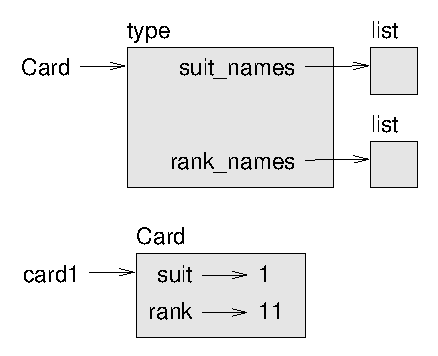
\includegraphics{figs/card1.eps}}
\afterfig

{\tt Card} is a class object, so it has type {\tt type}.  {\tt
card1} has type {\tt Card}.  (To save space, I didn't draw the
contents of \verb"suit_names" and \verb"rank_names").


\section{Comparing cards}
\label{comparecard}

\index{operator!conditional}
\index{conditional operator}

For built-in types, there are conditional operators
({\tt <}, {\tt >}, {\tt ==}, etc.)
that compare
values and determine when one is greater than, less than, or equal to
another.  For user-defined types, we can override the behavior of
the built-in operators by providing a method named
\verb"__cmp__".  

\verb"__cmp__" takes two parameters, {\tt self} and {\tt other},
and returns a positive number if the first object is greater, a
negative number if the second object is greater, and 0 if they are
equal to each other.

\index{override}
\index{operator overloading}

The correct ordering for cards is not obvious.
For example, which
is better, the 3 of Clubs or the 2 of Diamonds?  One has a higher
rank, but the other has a higher suit.  In order to compare
cards, you have to decide whether rank or suit is more important.

The answer might depend on what game you are playing, but to keep
things simple, we'll make the arbitrary choice that suit is more
important, so all of the Spades outrank all of the Diamonds,
and so on.

\index{cmp method@\_\_cmp\_\_ method}
\index{method!\_\_cmp\_\_}

With that decided, we can write \verb"__cmp__":

\beforeverb
\begin{verbatim}
# inside class Card:

    def __cmp__(self, other):
        # check the suits
        if self.suit > other.suit: return 1
        if self.suit < other.suit: return -1

        # suits are the same... check ranks
        if self.rank > other.rank: return 1
        if self.rank < other.rank: return -1

        # ranks are the same... it's a tie
        return 0    
\end{verbatim}
\afterverb
%
You can write this more concisely using tuple comparison:

\index{tuple!comparison}
\index{comparison!tuple}

\beforeverb
\begin{verbatim}
# inside class Card:

    def __cmp__(self, other):
        t1 = self.suit, self.rank
        t2 = other.suit, other.rank
        return cmp(t1, t2)
\end{verbatim}
\afterverb
%
The built-in function {\tt cmp} has the same interface as
the method \verb"__cmp__": it takes two values and returns
a positive number if the first is larger, a negative number
if the second is larger, and 0 if they are equal.

\index{cmp function}
\index{function!cmp}


\begin{ex}
Write a \verb"__cmp__" method for Time objects.  Hint: you
can use tuple comparison, but you also might consider using
integer subtraction.

%    def __cmp__(self, other):
%        return time_to_int(self) - time_to_int(other)

%If {\tt self} is later than {\tt other}, the result is
%a positive number.  If {\tt other} is later, the result
%is negative.  And if {\tt self} and {\tt other} are equal
%(but not necessarily identical)
%the result is zero.

\end{ex}


\section{Decks}
\index{list!of objects}
\index{deck, playing cards}

Now that we have Cards, the next step is to define Decks.  Since a
deck is made up of cards, it is natural for each Deck to contain a
list of cards as an attribute.

\index{init method}
\index{method!init}

The following is a class definition for {\tt Deck}.  The
init method creates the attribute {\tt cards} and generates
the standard set of fifty-two cards:

\index{composition}
\index{loop!nested}

\index{Deck class}
\index{class!Deck}

\beforeverb
\begin{verbatim}
class Deck(object):

    def __init__(self):
        self.cards = []
        for suit in range(4):
            for rank in range(1, 14):
                card = Card(suit, rank)
                self.cards.append(card)
\end{verbatim}
\afterverb
%
The easiest way to populate the deck is with a nested loop.  The outer
loop enumerates the suits from 0 to 3.  The inner loop enumerates the
ranks from 1 to 13.  Each iteration
creates a new Card with the current suit and rank,
and appends it to {\tt self.cards}.

\index{append method}
\index{method!append}


\section{Printing the deck}
\label{printdeck}

\index{str method@\_\_str\_\_ method}
\index{method!\_\_str\_\_}

Here is a \verb"__str__" method for {\tt Deck}:

\beforeverb
\begin{verbatim}
#inside class Deck:

    def __str__(self):
        res = []
        for card in self.cards:
            res.append(str(card))
        return '\n'.join(res)
\end{verbatim}
\afterverb
%
This method demonstrates an efficient way to accumulate a large
string: building a list of strings and then using {\tt join}.
The built-in function {\tt str} invokes the \verb"__str__"
method on each card and returns the string representation.

\index{accumulator!string}
\index{string!accumulator}
\index{join method}
\index{method!join}
\index{newline}

Since we invoke {\tt join} on a newline character, the cards
are separated by newlines.  Here's what the result looks like:

\beforeverb
\begin{verbatim}
>>> deck = Deck()
>>> print deck
Ace of Clubs
2 of Clubs
3 of Clubs
...
10 of Spades
Jack of Spades
Queen of Spades
King of Spades
\end{verbatim}
\afterverb
%
Even though the result appears on 52 lines, it is
one long string that contains newlines.


\section{Add, remove, shuffle and sort}

To deal cards, we would like a method that
removes a card from the deck and returns it.
The list method {\tt pop} provides a convenient way to do that:

\index{pop method}
\index{method!pop}

\beforeverb
\begin{verbatim}
#inside class Deck:

    def pop_card(self):
        return self.cards.pop()
\end{verbatim}
\afterverb
%
Since {\tt pop} removes the {\em last} card in the list, we are
dealing from the bottom of the deck.  In real life bottom dealing is
frowned upon\footnote{See \url{wikipedia.org/wiki/Bottom_dealing}.},
but in this context it's ok.

\index{append method}
\index{method!append}

To add a card, we can use the list method {\tt append}:

\beforeverb
\begin{verbatim}
#inside class Deck:

    def add_card(self, card):
        self.cards.append(card)
\end{verbatim}
\afterverb
%
A method like this that uses another function without doing
much real work is sometimes called a {\bf veneer}.  The metaphor
comes from woodworking, where it is common to glue a thin
layer of good quality wood to the surface of a cheaper piece of
wood.

\index{veneer}

In this case we are defining a ``thin'' method that expresses
a list operation in terms that are appropriate for decks.

As another example, we can write a Deck method named {\tt shuffle}
using the function {\tt shuffle} from the {\tt random} module:

\index{random module}
\index{module!random}
\index{shuffle function}
\index{function!shuffle}

\beforeverb
\begin{verbatim}
# inside class Deck:
            
    def shuffle(self):
        random.shuffle(self.cards)
\end{verbatim}
\afterverb
%
Don't forget to import {\tt random}.

\begin{ex}
\index{sort method}
\index{method!sort}

Write a Deck method named {\tt sort} that uses the list method
{\tt sort} to sort the cards in a {\tt Deck}.  {\tt sort} uses
the \verb"__cmp__" method we defined to determine sort order.
\end{ex}



\section{Inheritance}

\index{inheritance}
\index{object-oriented programming}

The language feature most often associated with object-oriented
programming is {\bf inheritance}.  Inheritance is the ability to
define a new class that is a modified version of an existing
class.

\index{parent class}
\index{child class}
\index{class!child}
\index{subclass}
\index{superclass}

It is called ``inheritance'' because the new class inherits the
methods of the existing class.  Extending this metaphor, the existing
class is called the {\bf parent} and the new class is
called the {\bf child}.

As an example, let's say we want a class to represent a ``hand,''
that is, the set of cards held by one player.  A hand is similar to a
deck: both are made up of a set of cards, and both require operations
like adding and removing cards.

A hand is also different from a deck; there are operations we want for
hands that don't make sense for a deck.  For example, in poker we
might compare two hands to see which one wins.  In bridge, we might
compute a score for a hand in order to make a bid.

This relationship between classes---similar, but different---lends
itself to inheritance.  

The definition of a child class is like other class definitions,
but the name of the parent class appears in parentheses:

\index{parentheses!parent class in}
\index{parent class}
\index{class!parent}
\index{Hand class}
\index{class!Hand}

\beforeverb
\begin{verbatim}
class Hand(Deck):
    """represents a hand of playing cards"""
\end{verbatim}
\afterverb
%
This definition indicates that {\tt Hand} inherits from {\tt Deck};
that means we can use methods like \verb"pop_card" and \verb"add_card"
for Hands as well as Decks.

{\tt Hand} also inherits \verb"__init__" from {\tt Deck}, but
it doesn't really do what we want: instead of populating the hand
with 52 new cards, the init method for Hands should initialize
{\tt cards} with an empty list.

\index{override}
\index{init method}
\index{method!init}

If we provide an init method in the {\tt Hand} class, it overrides the
one in the {\tt Deck} class:

\beforeverb
\begin{verbatim}
# inside class Hand:

    def __init__(self, label=''):
        self.cards = []
        self.label = label
\end{verbatim}
\afterverb
%
So when you create a Hand, Python invokes this init method:

\beforeverb
\begin{verbatim}
>>> hand = Hand('new hand')
>>> print hand.cards
[]
>>> print hand.label
new hand
\end{verbatim}
\afterverb
%
But the other methods are inherited from {\tt Deck}, so we can use
\verb"pop_card" and \verb"add_card" to deal a card:

\beforeverb
\begin{verbatim}
>>> deck = Deck()
>>> card = deck.pop_card()
>>> hand.add_card(card)
>>> print hand
King of Spades
\end{verbatim}
\afterverb
%
A natural next step is to encapsulate this code in a method
called \verb"move_cards":

\index{encapsulation}

\beforeverb
\begin{verbatim}
#inside class Deck:

    def move_cards(self, hand, num):
        for i in range(num):
            hand.add_card(self.pop_card())
\end{verbatim}
\afterverb
%
\verb"move_cards" takes two arguments, a Hand object and the number of
cards to deal.  It modifies both {\tt self} and {\tt hand}, and
returns {\tt None}.

In some games, cards are moved from one hand to another,
or from a hand back to the deck.  You can use \verb"move_cards"
for any of these operations: {\tt self} can be either a Deck
or a Hand, and {\tt hand}, despite the name, can also be a {\tt Deck}.

\begin{ex}
Write a Deck method called \verb"deal_hands" that takes two
parameters, the number of hands and the number of cards per
hand, and that creates new Hand objects, deals the appropriate
number of cards per hand, and returns a list of Hand objects.
\end{ex}

Inheritance is a useful feature.  Some programs that would be
repetitive without inheritance can be written more elegantly
with it.  Inheritance can facilitate code reuse, since you can
customize the behavior of parent classes without having to modify
them.  In some cases, the inheritance structure reflects the natural
structure of the problem, which makes the program easier to
understand.

On the other hand, inheritance can make programs difficult to read.
When a method is invoked, it is sometimes not clear where to find its
definition.  The relevant code may be scattered among several modules.
Also, many of the things that can be done using inheritance can be
done as well or better without it.  


\section{Class diagrams}

So far we have seen stack diagrams, which show the state of
a program, and object diagrams, which show the attributes
of an object and their values.  These diagrams represent a snapshot
in the execution of a program, so they change as the program
runs.

They are also highly detailed; for some purposes, too
detailed.  A class diagrams is a more abstract representation
of the structure of a program.  Instead of showing individual
objects, it shows classes and the relationships between them.

There are several kinds of relationship between classes:

\begin{itemize}

\item Objects in one class might contain references to objects
in another class.  For example, each Rectangle contains a reference
to a Point, and each Deck contains references to many Cards.
This kind of relationship is called {\bf HAS-A}, as in, ``a Rectangle
has a Point.''

\item One class might inherit from another.  This relationship
is called {\bf IS-A}, as in, ``a Hand is a kind of a Deck.''

\item One class might depend on another in the sense that changes
in one class would require changes in the other.

\end{itemize}

\index{IS-A relationship}
\index{HAS-A relationship}
\index{class diagram}
\index{diagram!class}
\index{UML}

A {\bf class diagram} is a graphical representation of these
relationships\footnote{The diagrams I am using here are similar to UML
  (see \url{wikipedia.org/wiki/Unified_Modeling_Language}), with a few
  simplifications.}.  For example, this diagram shows the
relationships between {\tt Card}, {\tt Deck} and {\tt Hand}.

\beforefig
\centerline{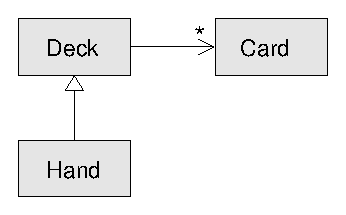
\includegraphics{figs/class1.eps}}
\afterfig

The arrow with a hollow triangle head represents an IS-A
relationship; in this case it indicates that Hand inherits
from Deck.

The standard arrow head represents a HAS-A
relationship; in this case a Deck has references to Card
objects.

\index{multiplicity (in class diagram)}

The star ({\tt *}) near the arrow head is a 
{\bf multiplicity}; it indicates how many Cards a Deck has.
A multiplicity can be a simple number, like {\tt 52}, a range,
like {\tt 5..7} or a star, which indicates that a Deck can
have any number of Cards.

A more detailed diagram might show that a Deck actually
contains a {\em list} of Cards, but built-in types
like list and dict are usually not included in class diagrams.


\section{Debugging}
\index{debugging}

Inheritance can make debugging a challenge because when you
invoke a method on an object, you might not know which method
will be invoked.

\index{polymorphism}

Suppose you are writing a function that works with Hand objects.
You would like it to work with all kinds of Hands, like
PokerHands, BridgeHands, etc.  If you invoke a method like
{\tt shuffle}, you might get the one defined in {\tt Deck},
but if any of the subclasses override this method, you'll
get that version instead.  

\index{flow of execution}

Any time you are unsure about the flow of execution through your
program, the simplest solution is to add print statements at the
beginning of the relevant methods.  If {\tt Deck.shuffle} prints a
message that says something like {\tt Running Deck.shuffle}, then as
the program runs it traces the flow of execution.

As an alternative, you could use this function, which takes an
object and a method name (as a string) and returns the class that
provides the definition of the method:

\beforeverb
\begin{verbatim}
def find_defining_class(obj, meth_name):
    for ty in type(obj).mro():
        if meth_name in ty.__dict__:
            return ty
\end{verbatim}
\afterverb
%
Here's an example:

\beforeverb
\begin{verbatim}
>>> hand = Hand()
>>> print find_defining_class(hand, 'shuffle')
<class 'Card.Deck'>
\end{verbatim}
\afterverb
%
So the {\tt shuffle} method for this Hand is the one in {\tt Deck}.

\index{mro method}
\index{method!mro}
\index{method resolution order}

\verb"find_defining_class" uses the {\tt mro} method to get the list
of class objects (types) that will be searched for methods.  ``MRO''
stands for ``method resolution order.''

\index{override}
\index{interface}
\index{precondition}
\index{postcondition}

Here's a program design suggestion: whenever you override a method,
the interface of the new method should be the same as the old.  It
should take the same parameters, return the same type, and obey the
same preconditions and postconditions.  If you obey this rule, you
will find that any function designed to work with an instance of a
superclass, like a Deck, will also work with instances of subclasses
like a Hand or PokerHand.

If you violate this rule, your code will collapse like (sorry)
a house of cards.


\section{Glossary}

\begin{description}

\item[encode:]  To represent one set of values using another
set of values by constructing a mapping between them.
\index{encode}

\item[class attribute:] An attribute associated with a class
object.  Class attributes are defined inside
a class definition but outside any method.
\index{class attribute}
\index{attribute!class}

\item[instance attribute:] An attribute associated with an
instance of a class.
\index{instance attribute}
\index{attribute!instance}

\item[veneer:] A method or function that provides a different
interface to another function without doing much computation.
\index{veneer}

\item[inheritance:] The ability to define a new class that is a
modified version of a previously defined class.
\index{inheritance}

\item[parent class:] The class from which a child class inherits.
\index{parent class}

\item[child class:] A new class created by inheriting from an
existing class; also called a ``subclass.''
\index{child class}
\index{class!child}

\item[IS-A relationship:] The relationship between a child class
and its parent class.
\index{IS-A relationship}

\item[HAS-A relationship:] The relationship between two classes
where instances of one class contain references to instances of
the other.
\index{HAS-A relationship}

\item[class diagram:] A diagram that shows the classes in a program
and the relationships between them.
\index{class diagram}
\index{diagram!class}

\item[multiplicity:] A notation in a class diagram that shows, for
a HAS-A relationship, how many references there are to instances
of another class.
\index{multiplicity (in class diagram)}

\end{description}


\section{Exercises}

\begin{ex}
\index{poker}


The following are the possible hands in poker, in increasing order
of value (and decreasing order of probability):

\begin{description}

\item[pair:] two cards with the same rank
\vspace{-0.05in}

\item[two pair:] two pairs of cards with the same rank
\vspace{-0.05in}

\item[three of a kind:] three cards with the same rank
\vspace{-0.05in}

\item[straight:] five cards with ranks in sequence (aces can
be high or low, so {\tt Ace-2-3-4-5} is a straight and so is {\tt
10-Jack-Queen-King-Ace}, but {\tt Queen-King-Ace-2-3} is not.)
\vspace{-0.05in}

\item[flush:] five cards with the same suit
\vspace{-0.05in}

\item[full house:] three cards with one rank, two cards with another
\vspace{-0.05in}

\item[four of a kind:] four cards with the same rank
\vspace{-0.05in}

\item[straight flush:] five cards in sequence (as defined above) and
with the same suit
\vspace{-0.05in}

\end{description}
%
The goal of these exercises is to estimate
the probability of drawing these various hands.

\begin{enumerate}

\item Download the following files from \url{thinkpython.com/code}:

\begin{description}

\item[{\tt Card.py}]: A complete version of the {\tt Card},
{\tt Deck} and {\tt Hand} classes in this chapter.

\item[{\tt PokerHand.py}]: An incomplete implementation of a class
that represents a poker hand, and some code that tests it.

\end{description}
%
\item If you run {\tt PokerHand.py}, it deals seven 7-card poker hands
and checks to see if any of them contains a flush.  Read this
code carefully before you go on.

\item Add methods to {\tt PokerHand.py} named \verb"has_pair",
\verb"has_twopair", etc. that return True or False according to
whether or not the hand meets the relevant criteria.  Your code should
work correctly for ``hands'' that contain any number of cards
(although 5 and 7 are the most common sizes).

\item Write a method named {\tt classify} that figures out
the highest-value classification for a hand and sets the
{\tt label} attribute accordingly.  For example, a 7-card hand
might contain a flush and a pair; it should be labeled ``flush''.

\item When you are convinced that your classification methods are
working, the next step is to estimate the probabilities of the various
hands.  Write a function in {\tt PokerHand.py} that shuffles a deck of
cards, divides it into hands, classifies the hands, and counts the
number of times various classifications appear.

\item Print a table of the classifications and their probabilities.
Run your program with larger and larger numbers of hands until the
output values converge to a reasonable degree of accuracy.  Compare
your results to the values at \url{wikipedia.org/wiki/Hand_rankings}.

\end{enumerate}
\end{ex}


\appendix

\chapter{Debugging}
\index{debugging}

Different kinds of errors can occur
in a program, and it is useful to distinguish among them
in order to track them down more quickly:

\begin{itemize}

\item Syntax errors are produced by Python when it is translating the
  source code into byte code.  They usually indicate that there is
  something wrong with the syntax of the program.  Example: Omitting
  the colon at the end of a {\tt def} statement yields the somewhat
  redundant message {\tt SyntaxError: invalid syntax}.

\item Runtime errors are produced by the interpreter if something goes
  wrong while the program is running.  Most runtime error messages
  include information about where the error occurred and what
  functions were executing.  

\item Semantic errors are problems with a program that runs without
  producing error messages but doesn't do the right thing.  Example:
  An expression may not be evaluated in the order you expect, yielding
  an incorrect result.

\end{itemize}

\index{syntax error}
\index{runtime error}
\index{semantic error}
\index{error!compile-time}
\index{error!syntax}
\index{error!runtime}
\index{error!semantic}
\index{exception}

The first step in debugging is to figure out which kind of
error you are dealing with.  Although the following sections are
organized by error type, some techniques are
applicable in more than one situation.


\section{Syntax errors}

\index{error message}

Syntax errors are usually easy to fix once you figure out what they
are.  Unfortunately, the error messages are often not helpful.
The most common messages are {\tt SyntaxError: invalid syntax} and
{\tt SyntaxError: invalid token}, neither of which is very informative.

On the other hand, the message does tell you where in the program the
problem occurred.  Actually, it tells you where Python
noticed a problem, which is not necessarily where the error
is.  Sometimes the error is prior to the location of the error
message, often on the preceding line.

\index{incremental development}
\index{development plan!incremental}

If you are building the program incrementally, you should have
a good idea about where the error is.  It will be in the last
line you added.

If you are copying code from a book, start by comparing
your code to the book's code very carefully.  Check every character.
At the same time, remember that the book might be wrong, so
if you see something that looks like a syntax error, it might be.

Here are some ways to avoid the most common syntax errors:

\index{syntax}

\begin{enumerate}

\item Make sure you are not using a Python keyword for a variable name.

\index{keyword}

\item Check that you have a colon at the end of the header of every
compound statement, including {\tt for}, {\tt while},
{\tt if}, and {\tt def} statements.

\index{header}
\index{colon}

\item Make sure that any strings in the code have matching
quotation marks.

\index{quotation mark}

\item If you have multiline strings with triple quotes (single or double), make
sure you have terminated the string properly.  An unterminated string
may cause an {\tt invalid token} error at the end of your program,
or it may treat the following part of the program as a string until it
comes to the next string.  In the second case, it might not produce an error
message at all!

\index{multiline string}
\index{string!multiline}

\item An unclosed opening operator---\verb+(+, \verb+{+, or
  \verb+[+---makes Python continue with the next line as part of the
  current statement.  Generally, an error occurs almost immediately in
  the next line.

\item Check for the classic {\tt =} instead of {\tt ==} inside
a conditional.

\index{conditional}

\item Check the indentation to make sure it lines up the way it
is supposed to.  Python can handle space and tabs, but if you mix
them it can cause problems.  The best way to avoid this problem
is to use a text editor that knows about Python and generates
consistent indentation.

\index{indentation}
\index{whitespace}

\end{enumerate}

If nothing works, move on to the next section...


\subsection{I keep making changes and it makes no difference.}

If the interpreter says there is an error and you don't see it, that
might be because you and the interpreter are not looking at the same
code.  Check your programming environment to make sure that the
program you are editing is the one Python is trying to run.

If you are not sure, try putting an obvious and deliberate syntax
error at the beginning of the program.  Now run it again.  If the
interpreter doesn't find the new error, you are not running the
new code.

There are a few likely culprits:

\begin{itemize}

\item You edited the file and forgot to save the changes before
running it again.  Some programming environments do this
for you, but some don't.

\item You changed the name of the file, but you are still running
the old name.

\item Something in your development environment is configured
incorrectly.

\item If you are writing a module and using {\tt import},
make sure you don't give your module the same name as one
of the standard Python modules.

\index{module!reload}
\index{reload function}
\index{function!reload}

\item If you are using {\tt import} to read a module, remember
that you have to restart the interpreter or use {\tt reload}
to read a modified file.  If you import the module again, it
doesn't do anything.

\end{itemize}

If you get stuck and you can't figure out what is going on, one
approach is to start again with a new program like ``Hello, World!,''
and make sure you can get a known program to run.  Then gradually add
the pieces of the original program to the new one.


\section{Runtime errors}

Once your program is syntactically correct,
Python can compile it and at least start running it.  What could
possibly go wrong?


\subsection{My program does absolutely nothing.}

This problem is most common when your file consists of functions and
classes but does not actually invoke anything to start execution.
This may be intentional if you only plan to import this module to
supply classes and functions.

If it is not intentional, make sure that you
are invoking a function to start execution, or execute one from
the interactive prompt.  Also see the ``Flow of Execution'' section
below.


\subsection{My program hangs.}
\index{infinite loop}
\index{hanging}

If a program stops and seems to be doing nothing, it is ``hanging.''
Often that means that it is caught in an infinite loop.  
If there is a particular loop that you suspect is the
problem, add a {\tt print} statement immediately before the loop that says
``entering the loop'' and another immediately after that says
``exiting the loop.''

\index{infinite loop}
\index{loop!infinite}
\index{condition}
\index{loop!condition}

Run the program.  If you get the first message and not the second,
you've got an infinite loop.  
If you think you have an infinite loop and you think you know
what loop is causing the problem, add a {\tt print} statement 
inside the loop as the last statement in the loop
loop that prints the values of the variables in
the condition and the value of the condition.

For example:

\beforeverb
\begin{verbatim}
while x > 0 and y < 0 :
    # do something to x
    # do something to y

    print  'x: ', x
    print  'y: ', y
    print  'condition: ', (x > 0 and y < 0)
\end{verbatim}
\afterverb
%
Now when you run the program, you will see three lines of output
for each time through the loop.  The last time through the
loop, the condition should be {\tt false}.  If the loop keeps
going, you will be able to see the values of {\tt x} and {\tt y},
and you might figure out why they are not being updated correctly.

\subsubsection{Flow of Execution}
\index{flow of execution}

If you are not sure how the flow of execution is moving through
your program, add {\tt print} statements to the beginning of each
function with a message like ``entering function {\tt foo},'' where
{\tt foo} is the name of the function.

Now when you run the program, it will print a trace of each
function as it is invoked.


\subsection{When I run the program I get an exception.}
\index{exception}
\index{runtime error}

If something goes wrong during runtime, Python
prints a message that includes the name of the
exception, the line of the program where the problem occurred,
and a traceback.

\index{traceback}

The traceback identifies the function that is currently running,
and then the function that invoked it, and then the function that
invoked \emph{that}, and so on.  In other words, it traces the
sequence of function invocations that got you to where you are.  It
also includes the line number in your file where each of these
calls occurs.

The first step is to examine the place in the program where
the error occurred and see if you can figure out what happened.
These are some of the most common runtime errors:

\begin{description}

\item[NameError:]  You are trying to use a variable that doesn't
exist in the current environment.
Remember that local variables are local.  You
cannot refer to them from outside the function where they are defined.

\index{NameError}
\index{TypeError}
\index{exception!NameError}
\index{exception!TypeError}

\item[TypeError:] There are several possible causes:

\begin{itemize}

\item  You are trying to use a value improperly.  Example: indexing
a string, list, or tuple with something other than an integer.

\index{index}

\item There is a mismatch between the items in a format string and
the items passed for conversion.  This can happen if either the number
of items does not match or an invalid conversion is called for.

\index{format operator}
\index{operator!format}

\item You are passing the wrong number of arguments to a function or method.
For methods, look at the method definition and
check that the first parameter is {\tt self}.  Then look at the
method invocation; make sure you are invoking the method on an
object with the right type and providing the other arguments
correctly.

\end{itemize}

\item[KeyError:]  You are trying to access an element of a dictionary
using a key that the dictionary does not contain.

\index{KeyError}
\index{exception!KeyError}
\index{dictionary}

\item[AttributeError:] You are trying to access an attribute or method
that does not exist.  Check the spelling!  You can use
{\tt dir} to list the attributes that do exist.

If an AttributeError indicates that an object has {\tt NoneType},
that means that it is {\tt None}.  One common cause is forgetting
to return a value from a function; if you get to the end of
a function without hitting a {\tt return} statement, it returns
{\tt None}.  Another common cause is using the result from
a list method, like {\tt sort}, that returns {\tt None}.

\index{AttributeError}
\index{exception!AttributeError}

\item[IndexError:] The index you are using
to access a list, string, or tuple is greater than
its length minus one.  Immediately before the site of the error,
add a {\tt print} statement to display
the value of the index and the length of the array.
Is the array the right size?  Is the index the right value?

\index{IndexError}
\index{exception!IndexError}

\end{description}

\index{debugger (pdb)}
\index{Python debugger (pdb)}
\index{pdb (Python debugger)}

The Python debugger ({\tt pdb}) is useful for tracking down
Exceptions because it allows you to examine the state of the
program immediately before the error.  You can read
about {\tt pdb} at \url{docs.python.org/lib/module-pdb.html}.


\subsection{I added so many {\tt print} statements I get inundated with
output.}

\index{print statement}
\index{statement!print}

One of the problems with using {\tt print} statements for debugging
is that you can end up buried in output.  There are two ways
to proceed: simplify the output or simplify the program.

To simplify the output, you can remove or comment out {\tt print}
statements that aren't helping, or combine them, or format
the output so it is easier to understand.

To simplify the program, there are several things you can do.  First,
scale down the problem the program is working on.  For example, if you
are searching a list, search a \emph{small} list.  If the program takes
input from the user, give it the simplest input that causes the
problem.

\index{dead code}

Second, clean up the program.  Remove dead code and reorganize the
program to make it as easy to read as possible.  For example, if you
suspect that the problem is in a deeply nested part of the program,
try rewriting that part with simpler structure.  If you suspect a
large function, try splitting it into smaller functions and testing them
separately.

\index{testing!minimal test case}
\index{test case, minimal}

Often the process of finding the minimal test case leads you to the
bug.  If you find that a program works in one situation but not in
another, that gives you a clue about what is going on.

Similarly, rewriting a piece of code can help you find subtle
bugs.  If you make a change that you think shouldn't affect the
program, and it does, that can tip you off.


\section{Semantic errors}
\index{semantic error}
\index{error!semantic}

In some ways, semantic errors are the hardest to debug,
because the interpreter provides no information
about what is wrong.  Only you know what the program is supposed to
do.

The first step is to make a connection between the program
text and the behavior you are seeing.  You need a hypothesis
about what the program is actually doing.  One of the things
that makes that hard is that computers run so fast.

You will often wish that you could slow the program down to human
speed, and with some debuggers you can.  But the time it takes to
insert a few well-placed {\tt print} statements is often short compared to
setting up the debugger, inserting and removing breakpoints, and
``stepping'' the program to where the error is occurring.

\subsection{My program doesn't work.}

You should ask yourself these questions:

\begin{itemize}

\item Is there something the program was supposed to do but
which doesn't seem to be happening?  Find the section of the code
that performs that function and make sure it is executing when
you think it should.

\item Is something happening that shouldn't?  Find code in
your program that performs that function and see if it is
executing when it shouldn't.

\item Is a section of code producing an effect that is not
what you expected?  Make sure that you understand the code in
question, especially if it involves invocations to functions or methods in
other Python modules.  Read the documentation for the functions you invoke.
Try them out by writing simple test cases and checking the results.

\end{itemize}

In order to program, you need to have a mental model of how
programs work.  If you write a program that doesn't do what you expect,
very often the problem is not in the program; it's in your mental
model.

\index{model, mental}
\index{mental model}

The best way to correct your mental model is to break the program
into its components (usually the functions and methods) and test
each component independently.  Once you find the discrepancy
between your model and reality, you can solve the problem.

Of course, you should be building and testing components as you
develop the program.  If you encounter a problem,
there should be only a small amount of new code
that is not known to be correct.


\subsection{I've got a big hairy expression and it doesn't
do what I expect.}

\index{expression!big and hairy}
\index{big, hairy expression}

Writing complex expressions is fine as long as they are readable,
but they can be hard to debug.  It is often a good idea to
break a complex expression into a series of assignments to
temporary variables.

For example:

\beforeverb
\begin{verbatim}
self.hands[i].addCard(self.hands[self.findNeighbor(i)].popCard())
\end{verbatim}
\afterverb
%
This can be rewritten as:

\beforeverb
\begin{verbatim}
neighbor = self.findNeighbor(i)
pickedCard = self.hands[neighbor].popCard()
self.hands[i].addCard(pickedCard)
\end{verbatim}
\afterverb
%
The explicit version is easier to read because the variable
names provide additional documentation, and it is easier to debug
because you can check the types of the intermediate variables
and display their values.

\index{temporary variable}
\index{variable!temporary}
\index{order of operations}
\index{precedence}

Another problem that can occur with big expressions is
that the order of evaluation may not be what you expect.
For example, if you are translating the expression
$\frac{x}{2 \pi}$ into Python, you might write:

\beforeverb
\begin{verbatim}
y = x / 2 * math.pi
\end{verbatim}
\afterverb
%
That is not correct because multiplication and division have
the same precedence and are evaluated from left to right.
So this expression computes $x \pi / 2$.

A good way to debug expressions is to add parentheses to make
the order of evaluation explicit:

\beforeverb
\begin{verbatim}
 y = x / (2 * math.pi)
\end{verbatim}
\afterverb
%
Whenever you are not sure of the order of evaluation, use
parentheses.  Not only will the program be correct (in the sense
of doing what you intended), it will also be more readable for
other people who haven't memorized the rules of precedence.


\subsection{I've got a function or method that doesn't return what I
expect.}
\index{return statement}
\index{statement!return}

If you have a {\tt return} statement with a complex expression,
you don't have a chance to print the {\tt return} value before
returning.  Again, you can use a temporary variable.  For
example, instead of:

\beforeverb
\begin{verbatim}
return self.hands[i].removeMatches()
\end{verbatim}
\afterverb
%
you could write:

\beforeverb
\begin{verbatim}
count = self.hands[i].removeMatches()
return count
\end{verbatim}
\afterverb
%
Now you have the opportunity to display the value of
{\tt count} before returning.


\subsection{I'm really, really stuck and I need help.}

First, try getting away from the computer for a few minutes.
Computers emit waves that affect the brain, causing these
symptoms:

\begin{itemize}

\item Frustration and rage.

\index{frustration}
\index{rage}
\index{debugging!emotional response}
\index{emotional debugging}

\item Superstitious beliefs (``the computer hates me'') and
magical thinking (``the program only works when I wear my
hat backward'').

\index{debugging!superstition}
\index{superstitious debugging}

\item Random walk programming (the attempt to program by writing
every possible program and choosing the one that does the right
thing).

\index{random walk programming}
\index{development plan!random walk programming}

\end{itemize}

If you find yourself suffering from any of these symptoms, get
up and go for a walk.  When you are calm, think about the program.
What is it doing?  What are some possible causes of that
behavior?  When was the last time you had a working program,
and what did you do next?

Sometimes it just takes time to find a bug.  I often find bugs
when I am away from the computer and let my mind wander.  Some
of the best places to find bugs are trains, showers, and in bed,
just before you fall asleep.


\subsection{No, I really need help.}

It happens.  Even the best programmers occasionally get stuck.
Sometimes you work on a program so long that you can't see the
error.  A fresh pair of eyes is just the thing.

Before you bring someone else in, make sure you are prepared.
Your program should be as simple
as possible, and you should be working on the smallest input
that causes the error.  You should have {\tt print} statements in the
appropriate places (and the output they produce should be
comprehensible).  You should understand the problem well enough
to describe it concisely.

When you bring someone in to help, be sure to give
them the information they need:

\begin{itemize}

\item If there is an error message, what is it
and what part of the program does it indicate?

\item What was the last thing you did before this error occurred?
What were the last lines of code that you wrote, or what is
the new test case that fails?

\item What have you tried so far, and what have you learned?

\end{itemize}

When you find the bug, take a second to think about what you
could have done to find it faster.  Next time you see something
similar, you will be able to find the bug more quickly.

Remember, the goal is not just to make the program
work.  The goal is to learn how to make the program work.



\chapter{Contributor List}
\section*{Contributor List for ``Python for Informatics''}

Bruce Shields for copy editing early drafts,
Sarah Hegge,
Steven Cherry,
Sarah Kathleen Barbarow,
Andrea Parker,
Radaphat Chongthammakun,
Megan Hixon,
Kirby Urner,
Sarah Kathleen Barbrow,
Katie Kujala,
Noah Botimer,
Emily Alinder,
Mark Thompson-Kular,
James Perry,
Eric Hofer,
Eytan Adar,
Peter Robinson,
Deborah J. Nelson,
Jonathan C. Anthony,
Eden Rassette,
Jeannette Schroeder,
Justin Feezell,
Chuanqi Li,
Gerald Gordinier,
Gavin Thomas Strassel,
Ryan Clement,
Alissa Talley,
Caitlin Holman,
Yong-Mi Kim,
Karen Stover,

% CONTRIB

\section*{Contributor List for ``Think Python''}

\index{contributors}

(Allen B. Downey)

More than 100 sharp-eyed and thoughtful readers have sent in
suggestions and corrections over the past few years.  Their
contributions, and enthusiasm for this project, have been a
huge help.

For the detail on the nature of each of the contributions from
these individuals, see the ``Think Python'' text.

Lloyd Hugh Allen,
Yvon Boulianne,
Fred Bremmer,
Jonah Cohen,
Michael Conlon,
Benoit Girard,
Courtney Gleason and Katherine Smith,
Lee Harr,
James Kaylin,
David Kershaw,
Eddie Lam,
Man-Yong Lee,
David Mayo,
Chris McAloon,
Matthew J. Moelter,
Simon Dicon Montford,
John Ouzts,
Kevin Parks,
David Pool,
Michael Schmitt,
Robin Shaw,
Paul Sleigh,
Craig T. Snydal,
Ian Thomas,
Keith Verheyden,
Peter Winstanley,
Chris Wrobel,
Moshe Zadka,
Christoph Zwerschke,
James Mayer,
Hayden McAfee,
Angel Arnal,
Tauhidul Hoque and Lex Berezhny,
Dr. Michele Alzetta,
Andy Mitchell,
Kalin Harvey,
Christopher P. Smith,
David Hutchins,
Gregor Lingl,
Julie Peters,
Florin Oprina,
D.~J.~Webre,
Ken,
Ivo Wever,
Curtis Yanko,
Ben Logan,
Jason Armstrong,
Louis Cordier,
Brian Cain,
Rob Black,
Jean-Philippe Rey at Ecole Centrale Paris,
Jason Mader at George Washington University made a number
Jan Gundtofte-Bruun,
Abel David and Alexis Dinno,
Charles Thayer,
Roger Sperberg,
Sam Bull,
Andrew Cheung,
C. Corey Capel,
Alessandra,
Wim Champagne,
Douglas Wright,
Jared Spindor,
Lin Peiheng,
Ray Hagtvedt,
Torsten H\"{u}bsch,
Inga Petuhhov,
Arne Babenhauserheide,
Mark E. Casida,
Scott Tyler,
Gordon Shephard,
Andrew Turner,
Adam Hobart,
Daryl Hammond and Sarah Zimmerman,
George Sass,
Brian Bingham,
Leah Engelbert-Fenton,
Joe Funke,
Chao-chao Chen,
Jeff Paine,
Lubos Pintes,
Gregg Lind and Abigail Heithoff,
Max Hailperin,
Chotipat Pornavalai,
Stanislaw Antol,
Eric Pashman,
Miguel Azevedo,
Jianhua Liu,
Nick King,
Martin Zuther,
Adam Zimmerman,
Ratnakar Tiwari,
Anurag Goel,
Kelli Kratzer,
Mark Griffiths,
Roydan Ongie,
Patryk Wolowiec,
Mark Chonofsky,
Russell Coleman,
Wei Huang,
Karen Barber,
Nam Nguyen,
St\'{e}phane Morin,
and
Paul Stoop.

\normalsize

\printindex

\clearemptydoublepage


\end{document}
